\documentclass[UTF8,zihao=-4,openany]{ctexrep}
\input{config/packages}
\usepackage[a4paper,left=2.5cm,right=2.3cm,top=2.4cm,bottom=2.4cm,headheight=15pt,headsep=0.6cm,footskip=1.0cm]{geometry}
\usepackage{fancyhdr}
\input{config/commands}
\input{config/format}
\input{config/metadata}
\input{config/symbols}
\setlength{\textfloatsep}{12pt plus 2pt minus 2pt}
\setlength{\floatsep}{10pt plus 2pt minus 2pt}
\setlength{\intextsep}{10pt plus 2pt minus 2pt}
\renewcommand{\topfraction}{0.90}
\renewcommand{\bottomfraction}{0.80}
\renewcommand{\textfraction}{0.08}
\renewcommand{\floatpagefraction}{0.72}
\setcounter{topnumber}{3}
\setcounter{bottomnumber}{2}
\setcounter{totalnumber}{5}
\pagestyle{fancy}
\fancyhf{}
\fancyfoot[C]{\thepage}
\renewcommand{\headrulewidth}{0pt}
\fancypagestyle{plain}{
  \fancyhf{}
  \fancyfoot[C]{\thepage}
  \renewcommand{\headrulewidth}{0pt}
}
\begin{document}
\maketitle
\tableofcontents
\listoffigures
\listoftables
\chapter{编制目的与任务要求}\label{chap:purpose}
% REQUIREMENT-SOURCE: C:/Users/V3169/Desktop/Project/SCL_Channel_Coding_Design/任务要求/附件3-信道编码、交织与译码方案及仿真分析.pdf

\section{编制目的}

本研究面向类星导航信号体制中的低速导航电文和高速导航电文，分析电文从有效信息输入到接收端恢复之间的信道编码、译码与交织方案。研究范围及基本参数依据项目任务说明文件确定，涵盖两类业务、三类编码和七组验证任务：低速电文采用BCH码，高速电文比较卷积码与 5G NR LDPC 两类码。

不同业务对冗余、可靠性和处理时延的容忍度不同，因而需要灵活调整使用的码型。低速电文更强调接收稳健性、实现简单和译码时延可控；高速电文除可靠性外，还要考虑连续处理、有效吞吐、软判决收益以及迭代译码造成的时间波动。

多信道、译码算法和交织分别回答不同问题。多信道试验检查既定码型遇到 AWGN、多径、频偏、遮挡或突发错误时的性能变化；译码算法对比关注同一码字条件下的纠错能力、运算量、存储量和时间；交织试验只考察错误离散化对 BCH 或卷积码的改善，并记录额外缓冲和时延。

\section{业务对象与设计范围}

研究对象分为低速电文与高速电文两类。这里的“低速”和“高速”表示业务分类；

低速电文包含 \SI{200}{bit} 和 \SI{300}{bit} 两种原始有效长度，只研究 BCH。BCH码的设计同时保留分组和整块两种组织方式：分组方案把一帧电文拆成若干短 BCH 信息块，整块方案把完整信息比特适配为较长的缩短 BCH 码字。比较内容包括两种编码方式的可靠性、不同信道下的稳健性、实现复杂度和译码时间。

高速电文只保留 \SI{300}{bit}信息比特。卷积码承担连续处理和 Viterbi 译码方案，5G NR LDPC 是短块迭代译码的候选方案；两者在接近码率、相同信息比特和明确的信道条件下比较实时性、冗余和译码代价。

\section{电文输入与编码约束}

表~\ref{tab:requirement-constraints}列出输入规模、候选码型和结果形式等设计约束，并说明相应处理口径；

\begin{table}[htbp]
  \centering
  \small
  \caption{主要设计约束及报告处理方式}
  \label{tab:requirement-constraints}
  \begin{tabular}{p{0.16\textwidth}p{0.36\textwidth}p{0.38\textwidth}}
    \toprule
    项目 & 要求 & 处理方式 \\
    \midrule
    输入长度 & 低速电文约 \SI{200}{bit}、\SI{300}{bit}；高速电文只保留约 \SI{300}{bit}（第1页） & 统一按 payload 记录，附加位另列 \\
    总码长 & 单个编码块编码后总码长不超过 \SI{1000}{bit}（第1页） & 逐任务核对编码块输出和实际发送长度，不用母码参数代替 \\
    码率 & 覆盖 $1/2$、$2/3$、$3/4$、$4/5$ 附近码率（第1页） & 报告 $K_{\mathrm{payload}}/N_{\mathrm{encoded}}$ 的实际值 \\
    BCH & 分组短码与整块缩短 BCH 对比（第2--3页） & 用于 S1、S2、S6、S7 的低速候选 \\
    卷积码 & 硬/软 Viterbi，整块及按时隙处理（第3--4页） & 用于 S3、S5、S6、S7 的高速候选 \\
    LDPC & BG2 短块，BP/NMS，迭代及提前停止（第4--5页） & 用于 S4、S5、S6；Direct 实现边界单列 \\
    交织 & 独立测试；LDPC 不配置交织（第6页） & 基础曲线默认无交织，仅在 S7 突发错误场景启用 \\
    输出 & BER、FER、成功率、平均/最大时延、复杂度等曲线与表格（第7页） & 保存原始统计、参数表、图源字段及适用场景 \\
    \bottomrule
  \end{tabular}
\end{table}

码率中的“附近”意味着短块适配后允许与目标的码率存在微小的差异。BCH 缩短、卷积码尾比特和打孔、LDPC filler 或速率匹配都会改变最终长度。

\section{S1--S7仿真任务及其目的}

七项任务构成由码内筛选到专题验证的顺序。表~\ref{tab:s1-s7-purpose}列的是各任务的控制变量和输出用途，不预写尚未在对应章节审计的性能结论。

\begin{table}[htbp]
  \centering
  \scriptsize
  \caption{S1--S7 仿真任务、控制变量与用途}
  \label{tab:s1-s7-purpose}
  \begin{tabular}{p{0.06\textwidth}p{0.20\textwidth}p{0.25\textwidth}p{0.20\textwidth}p{0.20\textwidth}}
    \toprule
    任务 & 输入和候选 & 主要控制变量 & 输出 & 任务目的 \\
    \midrule
    S1 & 200/300 bit BCH，分组与整块 & 码长、码率、分组数、纠错能力 & BER、FER、成功状态、时延 & 在 BCH 内部筛选低速候选，供 S2、S6、S7 使用 \\
    S2 & S1 保留的 BCH & AWGN、多径、频偏、遮挡、突发错误 & 信道损失、FER、突发敏感性 & 检查低速候选的信道适应性 \\
    S3 & 300 bit 卷积码 & 码率、硬/软判决、量化、回溯、滑窗、时隙组织 & BER、FER、有效吞吐、首输出及译码时间 & 筛选高速卷积码候选 \\
    S4 & 300 bit BG2 Direct LDPC & 目标码长、BP/NMS、迭代上限、提前停止 & BER、FER、迭代、复杂度、时延 & 筛选高速 LDPC 候选 \\
    S5 & S3/S4 高速候选 & 接近码率、相同 payload、不同信道 & BER、FER、时延和鲁棒性 & 比较卷积码与 LDPC 的场景适用性 \\
    S6 & 固定码长与信道的三类码 & 只替换译码规则 & 性能、操作计数、存储、平均/最大时间 & 分离译码算法本身的收益和代价 \\
    S7 & 固定 BCH 或卷积码方案 & 交织器、交织深度、突发长度 & 突发容限、FER 改善、附加时延 & 评价交织；LDPC 仅作无交织基线 \\
    \bottomrule
  \end{tabular}
\end{table}

S1、S3、S4先在各自码型内部减少候选数量，避免把未经筛选的参数组合全部带入跨方案比较。S2和S5随后施加多信道条件，分别检验低速 BCH 和高速候选。S6固定编码与信道条件后只比较译码器，S7固定编码方案后只改变交织配置。这样可以把码型选择、信道适应性、译码实现和交织收益拆成可解释的四类差异。

\section{评价指标与成果形式}

\begin{table}[htbp]
  \centering
  \small
  \caption{评价指标的工程含义与使用边界}
  \label{tab:metric-categories}
  \begin{tabular}{p{0.16\textwidth}p{0.32\textwidth}p{0.42\textwidth}}
    \toprule
    类别 & 指标 & 注意 \\
    \midrule
    可靠性 & BER、FER、译码成功率、误纠、译码失败 & BER/FER 只统计恢复信息比特；\\
    传输效率 & 编码后长度、发送长度、实际码率、有效吞吐 & 附加位不进入信息比特；打孔后长度必须按实现解释 \\
    实现代价 & 操作计数、平均迭代次数、存储量、量化位宽 & 不用单一 CPU 时间替代算法复杂度 \\
    时延 & 平均、P95/P99、最大观测、首输出、结构时延、交织附加时延 & 仅在任务实际提供相应字段时报告；软件最大值不是硬件上界 \\
    场景表现 & 多信道损失、编码增益、交织改善、适用场景 & 比较点说明目标误码率、插值范围和共同控制条件 \\
    \bottomrule
  \end{tabular}
\end{table}

研究成果包括正式 BER/FER 主图、参数表、时延和复杂度表、场景说明以及可复现性记录。信噪比条件下的 BER、FER 曲线和表格以 Es/N0(符号信噪比) 为正式主图横轴。

\section{本章小结}

研究内容可归纳为四个相互关联的问题：码型和码长筛选、信道适应性、译码实现代价，以及交织对突发错误的改善。BCH、卷积码和 LDPC 分别完成码内候选筛选，再进入多信道、译码器和交织章节的比较。

\chapter{设计输入与总体方案}\label{chap:design}

\section{总体设计思路}

系统采用“公共仿真基础、可替换编码模块、场景化信道与统计配置”的组织方式。公共仿真模块（Common）位于三类编码模块之外，提供公共数据结构、BPSK、基础 AWGN、硬判决与 LLR、帧样本池、噪声样本池、信息比特的误码统计、停止控制、断点状态保存、分片合并及公共结果字段。该模块不生成 BCH、卷积码或 LDPC 校验关系，也不执行三类码的核心译码。

BCH、CC 和 LDPC 模块接收相同类型的信息比特和公共控制信息，但各自负责码长适配、编码、译码、信息比特恢复、算法状态以及任务专用指标。多径、频偏、遮挡和突发错误等扩展信道也由具体任务配置。

\section{数据对象与长度关系}

一帧电文经过适配、编码、调整和恢复时会出现多个长度。表~\ref{tab:data-length-objects}给出报告中的统一名称。

\begin{table}[htbp]
  \centering
  \small
  \caption{数据对象、长度符号及附加位关系}
  \label{tab:data-length-objects}
  \begin{tabular}{p{0.20\textwidth}p{0.20\textwidth}p{0.38\textwidth}p{0.14\textwidth}}
    \toprule
    符号 & 数据对象 & 含义 & 附加位关系 \\
    \midrule
    $K_{\mathrm{payload}}$ & 原始有效电文 & 用户需要恢复并用于 BER/FER 的比特 & 不含附加位 \\
    $K_{\mathrm{codec_input}}$ & 编码器输入 & 编码器实际接收的信息侧序列 & 可含 filler、CRC 或适配位 \\
    $N_{\mathrm{encoded}}$ & 编码输出 & Common 码率分母对应的最终编码长度 & 含校验、尾比特等 \\
    $N_{\mathrm{transmitted}}$ & 实际发送序列 & 映射到 BPSK 并进入信道的比特数 & 不含未发送缩短位和打孔位 \\
    $N_{\mathrm{received}}$ & 接收观测 & 进入硬判决或软信息计算的有效观测数 & 受接收处理影响 \\
    $K_{\mathrm{recovered}}$ & 恢复的信息比特 & 去除附加位后提交统计的比特序列 & 应等于 $K_{\mathrm{payload}}$ \\
    \bottomrule
  \end{tabular}
\end{table}

Filler 用于把短的信心比特补到编码结构要求的输入规模，不增加码率；CRC 用于检错或停止判断，也不属于信息比特；卷积码 tail 把编码器状态终止到约定状态，会增加编码输出长度；puncturing 从母码输出中删除部分比特，使实际码率提高；shortening 则把已知的信息位从发送序列中省略，接收端译码前按约定恢复这些位置。相同的 $K_{\mathrm{payload}}$ 因此可能对应不同的 $K_{\mathrm{codec\ input}}$、$N_{\mathrm{encoded}}$ 和 $N_{\mathrm{transmitted}}$。

\section{Common与编码模块的职责分工}

表~\ref{tab:common-codec-responsibility}按数据流列出 Common 和编码任务的边界。公共接口的存在表示三类码可以接入同一处理框架，不表示具体任务已经使用完全相同的信道、统计字段或停止参数。

\begin{table}[htbp]
  \centering
  \scriptsize
  \caption{Common 与三类编码任务的职责分工}
  \label{tab:common-codec-responsibility}
  \begin{tabular}{p{0.15\textwidth}p{0.35\textwidth}p{0.40\textwidth}}
    \toprule
    环节 & Common & 编码任务 \\
    \midrule
    信息比特的输入 & 确定性生成或从 Frame Pool 按帧索引读取 & 选择 200/300 bit 业务长度 \\
    码长适配 & 提供长度结构和公共字段 & 实现 filler、CRC、shortening、tail、puncturing \\
    编码 & 提供编码器接口 & 实现 BCH、卷积码或 BG2 Direct LDPC \\
    调制 & 固定实值 BPSK，0 映射 $+1$，1 映射 $-1$ & 通常直接复用 \\
    信道 & AWGN 实现和信道接口 & 增加多径、频偏、遮挡、突发错误等 \\
    解调 & 硬判决和未量化 LLR & 设置量化、裁剪、饱和或补偿 \\
    译码 & 提供输入/输出接口 & 实现查表、代数、Viterbi、BP 或 NMS \\
    信息比特的恢复 & 提供统计入口和长度校验 & 去除 filler、CRC、tail 等附加位 \\
    统计 & BER/FER、基础成功率、平均和最大时间 & 增加误纠、声明成功、迭代、复杂度、分位数等 \\
    \bottomrule
  \end{tabular}
\end{table}

\section{低速BCH处理路径}

低速路径从 \SI{200}{bit} 或 \SI{300}{bit} 信息比特开始。分组方案先按 BCH 信息位长度切分，不足一组时补入填充；整块方案把完整信息比特映射到较长 BCH 母码并执行缩短。编码产生一个或多个系统 BCH 码字，S7 可在编码后加入交织，随后进行 BPSK 和信道传输。接收端先硬判决，再在启用交织时去交织，之后执行查表或代数 BCH 译码，删除补入或缩短对应的非信息比特位置，最后提交固定长度的恢复结果。

分组方案会产生多个短码字，一帧 FER 的判定取决于所有子块恢复后的信息比特：只要任一信息比特位错误，整帧计为错误帧。整块方案的纠错边界、缩短位置和误纠状态由 BCH 章节结合实际实现说明。

\section{高速卷积码处理路径}

高速卷积码输入固定为 \SI{300}{bit}信息比特。整块组织可在电文末尾加入零尾，使移位寄存器回到约定状态；按时隙处理可保留连续状态，并通过滑窗 Viterbi 降低等待完整电文的时间。项目以 $1/2$ 母码为基础，通过打孔形成接近 $2/3$、$3/4$ 的发送码率。

接收端可将符号硬判为 0/1，也可把实值观测转换为 LLR 或量化值。硬、软 Viterbi 共用相同码字和接收符号时，差异主要来自分支度量；回溯深度、滑窗长度、软值位宽和饱和策略会同时影响存储、首输出和译码时间。整块零尾、连续状态和时隙分块还会改变结构时延。

\section{高速LDPC处理路径}

LDPC 路径只处理 \SI{300}{bit} 整块信息比特。编码模块依据 BG2 短块结构选择提升因子和使用的子矩阵，通过 filler 或 shortening 适配编码输入，并由 Direct QC-LDPC 编码器生成校验位。接收端计算软信息后，分别使用 Layered BP 和 Layered NMS 迭代译码；两者设置最大迭代次数，并在校验方程全部满足时允许提前停止。恢复阶段删除 filler 等非信息比特位置，只把原始 \SI{300}{bit} 范围交给公共统计。

本研究采用基于 5G NR BG2 结构的短块实现，其适用范围不包含完整的 5G NR 物理层传输链。

\section{统一通信与仿真链路}

三类码共享的上层数据流为：信息比特、码长适配、编码、可选交织、BPSK调制、信道、硬判决、去交织、译码、信息比特恢复和统计，如图\ref{fig:overall-scenario}所示。
% VISIO-ABSOLUTE-PATH: C:/Users/V3169/Desktop/Project/SCL_Channel_Coding_Design/Report/figures/visio/common/overall_scenario_architecture.png
\begin{figure}[htbp]
  \centering
  \includegraphics[width=0.90\textwidth]
  {figures/visio/common/overall_scenario_architecture.pdf}
  \caption{总体编码与仿真架构图}
  \label{fig:overall-scenario}
\end{figure}

结果整理保留内部 \texttt{ebN0Db} 和实际码率，并按每个点的码率计算正式横轴符号信噪比。该处理只增加展示坐标，不改动接收符号、错误计数或停止结果。下层控制信息通过帧索引、样本池身份和配置标识与各仿真点关联。

\begin{table}[htbp]
  \centering
  \small
  \caption{三类编码处理路径的主要组织差异}
  \label{tab:codec-path-comparison}
  \begin{tabular}{p{0.17\textwidth}p{0.23\textwidth}p{0.24\textwidth}p{0.26\textwidth}}
    \toprule
    项目 & BCH & 卷积码 & BG2 Direct LDPC \\
    \midrule
    业务输入 & 200/300 bit 低速 & 300 bit 高速 & 300 bit 高速 \\
    组织 & 分组或整块缩短 & 整块零尾或时隙连续 & 整块短块适配 \\
    码率调整 & 码型选择、缩短、填充 & 母码、尾比特、打孔 & 提升因子、filler、Direct 结构 \\
    译码输入 & 硬判决 & 硬比特或量化软信息 & LLR 或量化软信息 \\
    译码状态 & 无错、纠错、失败、误纠 & 路径输出及任务状态 & 校验满足、迭代上限等 \\
    交织 & S7 可选 & S7 可选 & 禁止配置 \\
    关键时延 & 子块处理与整帧完成 & 首输出、回溯、滑窗 & 迭代次数和尾部时间 \\
    \bottomrule
  \end{tabular}
\end{table}

\section{本章小结}

总体方案将公共数据与控制链同三类编译码实现分离：公共仿真模块固定可复用的基础调制、AWGN、随机样本、统计和一致性机制，编码模块负责码长适配、编译码及专用状态。低速 BCH、高速卷积码和高速LDPC因组织方式不同保留独立长度和时延字段；S1--S7依次完成码内筛选、场景检验、实现代价比较和交织分析。

\chapter{统一仿真方法}\label{chap:simulation}
% FORMULA-AUDIT: Report/evidence/round04/r3_formula_audit.csv

\section{Common公共仿真基础}

公共仿真模块（Common）为三类编码提供一致的仿真基础，不参与 BCH 生成多项式计算、卷积码状态转移或 LDPC 校验矩阵迭代。该模块提供统一类型和接口，固定实值 BPSK、基础 AWGN、硬判决和未量化 LLR 的定义，并通过帧样本池（Frame Pool）、噪声样本池（Noise Pool）、停止控制、断点状态保存（checkpoint）、分片合并和结果身份字段约束实验输入与输出。

公共实现解决的是“相同环节如何用同一种方式执行和记录”，不替代任务级说明。BCH、卷积码和 LDPC 的 filler、CRC、tail、puncturing、shortening、量化、译码状态、复杂度字段及扩展信道仍由各任务实现。

\section{帧结构与长度定义}

$K_{\mathrm{payload}}$ 是原始有效信息长度，也是 BER 分母中每帧贡献的比特数。$K_{\mathrm{codec_input}}$ 是编码器实际输入，可在信息比特之外包含 filler、CRC 或其他适配位。$N_{\mathrm{encoded}}$ 是 Common中计算码率所使用的编码输出长度；具体任务需要说明该字段是否已经完成打孔或速率匹配。$N_{\mathrm{transmitted}}$ 是实际映射到 BPSK 并进入信道的比特数，$K_{\mathrm{recovered}}$ 是去除附加位后的恢复长度。

Shortening 对应的已知位不进入发送序列；打孔位从母码输出中删除。

\begin{table}[htbp]
  \centering
  \scriptsize
  \caption{长度字段及附加位对各长度的影响}
  \label{tab:length-field-effects}
  \begin{tabular}{p{0.17\textwidth}p{0.16\textwidth}p{0.18\textwidth}p{0.18\textwidth}p{0.21\textwidth}}
    \toprule
    项目 & 是否属于 payload & 影响编码器输入 & 影响编码输出/发送 & 统计处理 \\
    \midrule
    filler & 否 & 增加 & 可能增加 & 恢复后删除 \\
    CRC & 否 & 通常增加 & 增加 & 可用于状态判断，不计 BER \\
    tail & 否 & 改变卷积码输入过程 & 增加输出 & 不计 payload BER \\
    puncturing & 否 & 不改变 & 删除部分母码比特 & 记录打孔后长度 \\
    shortening & 否 & 逻辑上补已知位 & 已知位不发送 & 译码前恢复约定位置 \\
    parity & 否 & 不属于信息侧 & 构成编码冗余 & 不直接计 payload BER \\
    \bottomrule
  \end{tabular}
\end{table}

\section{实际码率定义}

码率统一定义为：
\begin{equation}
  R=\frac{K_{\mathrm{payload}}}{N_{\mathrm{encoded}}}.
  \label{eq:actual-code-rate}
\end{equation}
分子不包含 filler、CRC 或 tail；分块方案的分母使用所有子块最终编码长度之和；打孔后若任务把打孔结果记为编码后的长度，分母使用打孔后长度。


\section{BPSK离散符号模型}

Common 的 BPSK 调制按逐比特实值映射：
\begin{equation}
  x_i=1-2c_i,qquad c_i\in\{0,1\},\quad x_i\in\{+1,-1\}.
  \label{eq:bpsk-mapping}
\end{equation}
式~\eqref{eq:bpsk-mapping}把比特 0 映射为 $+1$，把比特 1 映射为 $-1$，每个实际编码比特对应一个实值符号。

\section{Eb/N0下的AWGN实现}

\texttt{computeAwgnSigma} 的输入字段为 \texttt{ebN0\_dB}。函数先完成 dB 到线性量的转换：
\begin{equation}
  \gamma_b=10^{(E_b/N_0)_{\mathrm{dB}}/10}.
  \label{eq:ebn0-linear}
\end{equation}
式~\eqref{eq:ebn0-linear}完成 dB 到线性量的转换；随后调用式~\eqref{eq:actual-code-rate}计算实际码率，并返回标准差
\begin{equation}
  \sigma=\sqrt{\frac{1}{2R\gamma_b}},
  \qquad \sigma^2=\frac{1}{2R\gamma_b}.
  \label{eq:awgn-sigma}
\end{equation}
式~\eqref{eq:awgn-sigma}中的 $\sigma$ 进入下列接收模型：
\begin{equation}
  y_i=x_i+\sigma z_i,qquad z_i\sim\mathcal{N}(0,1).
  \label{eq:awgn-channel}
\end{equation}
式~\eqref{eq:awgn-channel}由 \texttt{applyAwgn} 实现；该函数要求符号向量和标准高斯向量等长，并拒绝非有限或非正的 $\sigma$。这里的 $\sigma$ 是标准差；Noise Pool 保存的是标准高斯 $z_i$，不是已经按某个 SNR 缩放的噪声。

上述闭式适用于调用 Common \texttt{computeAwgnSigma} 和 \texttt{applyAwgn} 的实值 BPSK--AWGN 处理链。

\section{Es/N0正式绘图口径}

信噪比条件下的 BER、FER 正式主图采用符号信噪比 $E_s/N_0$ 作为横轴，同时保留仿真输入 \texttt{ebN0Db}。在一编码比特对应一个 BPSK 符号且使用式~\eqref{eq:actual-code-rate}时，线性关系为
\begin{equation}
  \gamma_s=R\gamma_b.
  \label{eq:es-eb-linear}
\end{equation}
式~\eqref{eq:es-eb-linear}对应的 dB 换算为
\begin{equation}
  (E_s/N_0)_{\mathrm{dB}}
  =(E_b/N_0)_{\mathrm{dB}}+10\log_{10}R.
  \label{eq:es-eb-db}
\end{equation}

式~\eqref{eq:es-eb-db}的换算只增加 \texttt{esN0Db} 展示字段，原始 Eb/N0、噪声样本、$\sigma$、BER、FER、处理帧数和错误计数均保持不变。

\section{硬判决与软信息}

Common 的硬判决在零点明确归入 bit 0：
\begin{equation}
  \hat c_i=
  \begin{cases}
    0, & y_i\ge 0,\\
    1, & y_i<0.
  \end{cases}
  \label{eq:hard-decision}
\end{equation}
式~\eqref{eq:hard-decision}给出硬判决；实值 BPSK--AWGN 的未量化对数似然比为
\begin{equation}
  L_i=\ln\frac{\Pr(c_i=0\mid y_i)}{\Pr(c_i=1\mid y_i)}
     =\frac{2y_i}{\sigma^2}.
  \label{eq:llr}
\end{equation}
由式~\eqref{eq:llr}可知，正 LLR 倾向 bit 0，负 LLR 倾向 bit 1，绝对值表示可靠性。Common 基础接口不执行裁剪、定点量化或饱和；CC 和 LDPC 对软值的位宽、缩放、裁剪和溢出处理必须在任务章节说明。BCH 使用硬判决输入。

\section{BER、FER与译码状态}

公共错误统计只比较原始的信息比特和恢复后的信息比特：
\begin{align}
  \mathrm{BER}&=\frac{N_{b,\mathrm{err}}}{N_{b,\mathrm{payload}}},
  \label{eq:ber}\\
  \mathrm{FER}&=\frac{N_{f,\mathrm{err}}}{N_{f,\mathrm{processed}}},
  \label{eq:fer}\\
  S_{\mathrm{payload}}&=\frac{N_{f,\mathrm{correct}}}{N_{f,\mathrm{processed}}}
  =1-\mathrm{FER}.
  \label{eq:payload-success}
\end{align}
式~\eqref{eq:ber}和式~\eqref{eq:fer}分别按信息比特比特与帧计数。Common-04 \texttt{SummaryRow} 中的 \texttt{successRate} 对应式~\eqref{eq:payload-success}，即信息比特无误帧比例，不是译码器声明成功率。

\begin{table}[htbp]
  \centering
  \small
  \caption{译码器声明与payload结果的联合状态}
  \label{tab:decoder-status}
  \begin{tabular}{p{0.20\textwidth}p{0.20\textwidth}p{0.48\textwidth}}
    \toprule
    译码器声明 & 信息比特的结果 & 统计解释 \\
    \midrule
    成功 & 正确 & true success，同时可计入 declared success \\
    成功 & 错误 & miscorrection 或 undetected error，不能计入 payload success \\
    失败 & 错误 & decoder failure，同时是 frame error \\
    失败 & 正确 & 需由任务状态字段解释，基础 SummaryRow 不单列 \\
    \bottomrule
  \end{tabular}
\end{table}

\section{确定性随机噪声与公平比较}

Common 的每个标准高斯样本由完整 NoiseKey 决定：
\begin{equation}
  \mathcal{K}_{\mathrm{noise}}=
  (s_{\mathrm{master}},g_{\mathrm{noise}},f,i,v_{\mathrm{policy}}),
  \label{eq:noise-key}
\end{equation}
式~\eqref{eq:noise-key}的五个分量依次表示主噪声种子、噪声组、帧索引、符号索引和策略版本，对应源码中的 NoiseKey 字段。固定完整键产生相同样本，不依赖随机函数调用顺序。源码使用 SplitMix64 派生均匀字，并用 Box--Muller 变换生成标准高斯值。

\texttt{snrIndex} 和 Eb/N0 不直接进入 NoiseKey。不同 SNR 点通过式~\eqref{eq:awgn-sigma}改变 $\sigma$；是否跨 SNR 复用同一标准高斯底噪，取决于 \texttt{noiseGroupId} 及任务配置。不同 \texttt{frameIndex} 仍生成不同帧噪声，跨 SNR 复用不等于所有帧复用一条噪声。

卷积码的硬、软 Viterbi 的比较共享信息比特、母码输出和打孔结果，并采用相同的接收符号（\texttt{receivedSymbols}）。两种方案仅替换译码输入和分支度量。LDPC BP/NMS 共同接入、码字、校验矩阵、噪声和 LLR，只替换校验节点更新规则。共享随机样本使结果差异不再同时混入另一组 Monte Carlo 噪声。

\section{帧池和噪声池}

Noise Pool 保存未缩放的标准高斯样本，格式为 float64 little-endian，生成算法标识为 \texttt{splitmix64\_box\_muller\_v1}。每个二进制分片含版本化头字段，包括首帧、帧数、每帧符号数、主种子、噪声组和策略版本。manifest 要求连续帧范围、分片 SHA-256 和 overall hash，\texttt{noisePoolId} 取 overall hash 的前16个十六进制字符；读取时同时复核文件 hash 和头字段。

\section{仿真停止控制}

Common 的正式停止配置包含三项参数。最少帧数为 \texttt{minFrames=1000}，目标错误帧数为 \texttt{targetFrameErrors=200}，每点最大帧数为 \texttt{maxFrames=50000}。\texttt{evaluateStop} 的实际判断顺序如下：

\begin{verbatim}
if processedFrames >= maxFrames:
    MAX_FRAMES
elif processedFrames < minFrames:
    CONTINUE
elif frameErrors >= targetFrameErrors:
    TARGET_FRAME_ERRORS
else:
    CONTINUE
\end{verbatim}

最小帧数防止在错误较多的点过早停止；达到最小帧数后，目标错误帧数提供基本的错误事件数量；最大帧数限制高 SNR 点或低错误率点的计算量。

\section{时延统计口径}

\begin{table}[htbp]
  \centering
  \scriptsize
  \caption{Common基础时延字段、实际计时边界和限制}
  \label{tab:common-latency-fields}
  \begin{tabular}{p{0.24\textwidth}p{0.38\textwidth}p{0.10\textwidth}p{0.20\textwidth}}
    \toprule
    指标 & Common-04 identity pipeline实际边界 & 提供 & 限制 \\
    \midrule
    \texttt{avgEncodeTimeUs} & 信息比特生成/Frame Pool读取、编码、BPSK & 是 & 不是纯编码时间 \\
    \texttt{avgChannelTimeUs} & 噪声生成/Noise Pool读取及 AWGN 叠加 & 是 & 包含池读取或生成 \\
    \texttt{avgDecodeTimeUs} & 硬判决，或 LLR 计算后按符号判决 & 是 & identity 基线不是码译码器 \\
    \texttt{maxDecodeTimeUs} & 单帧上述 decode 阶段最大观测值 & 是 & 软件观测最大值 \\
    \texttt{avgRecoveryTimeUs} & 从 decoded 序列截取 payload & 是 & 具体码型恢复更复杂 \\
    \texttt{avgTotalTimeUs} & 单帧主链路起点至恢复完成 & 是 & 受平台与调度影响 \\
    \texttt{maxTotalTimeUs} & 单帧 total 最大观测值 & 是 & 不等于硬件确定上界 \\
    \bottomrule
  \end{tabular}
\end{table}

Common-01 将理想算法计时定义为不包含帧池和噪声文件读取；Common-04 identity pipeline 的实际函数边界包含这些操作。

\section{本章小结}

公共仿真模块固定了 payload/encoded 码率、实值 BPSK、Eb/N0 驱动的 AWGN、硬判决、LLR、payload BER/FER、确定性随机样本、正式停止控制以及基础断点状态、分片和结果身份。正式图按每个点的实际码率将内部 Eb/N0 转换为 Es/N0，原始统计保持不变。第4章以后的各编码与专题分析补充发送长度、附加位、扩展译码状态、量化、专用时延、复杂度和特殊信道信息，并逐项说明与公共定义的对应关系。

\chapter{BCH编码方案与仿真分析}\label{chap:bch}

\section{BCH低速电文编码设计目标}

本章针对长度为200 bit和300 bit的低速二进制电文，研究Bose--Chaudhuri--Hocquenghem（BCH）码的编码组织、软件实现和信道适应性。此类电文的数据量较小，但通常要求整帧正确交付；只要任一信息比特恢复错误，该帧就不能作为有效业务电文使用。因此，方案评价以帧错误率（Frame Error Rate，FER）为主，以比特错误率（Bit Error Rate，BER）、发送长度、实际码率和软件译码时间为辅助指标。

设计工作围绕两条路线展开。第一条路线把原始电文划分为若干11 bit信息组，各组独立采用BCH(15,11)编码，主要特点是结构简单、单组译码开销小。第二条路线把一帧信息装入较长的BCH母码，通过缩短获得与业务长度相适应的码字，利用较大的整块纠错能力提高可靠性。两条路线采用相同的二进制相移键控（Binary Phase Shift Keying，BPSK）调制和硬判决条件，使比较重点落在编码组织与纠错能力本身。

除加性高斯白噪声（Additive White Gaussian Noise，AWGN）基准外，本章还考察固定多径、频偏造成的帧内相位累积、连续遮挡以及连续突发翻转。研究目标不是给出脱离使用条件的单一“最优码”，而是回答三个工程问题：在相同信息长度下，冗余和纠错能力如何影响可靠性；简单查表译码与长码代数译码需要付出多大软件代价；当错误从分散形态转为局部集中形态时，单纯增强BCH码是否仍然有效。

\section{BCH编码组织方案}

\subsection{分组BCH方案}

分组方案以11 bit为一个信息组，逐组采用可纠正单个错误的BCH(15,11)系统码。若最后一组不足11 bit，则在信息尾部加入已知零作为填充位；接收端译码并拼接各组信息后，再删除填充位，得到原始电文。200 bit电文被划分为19组，加入9个填充位，发送长度为285 bit；300 bit电文被划分为28组，加入8个填充位，发送长度为420 bit。

对每个信息组，系统编码可写为
\begin{equation}
  c(x)=x^{n-k}m(x)+r(x),
\end{equation}
其中，$m(x)$为信息多项式，$r(x)$为$x^{n-k}m(x)$除以生成多项式所得的余式。信息位在码字中保持可见，便于检查编码与译码接口。由于每个子码字只能保证纠正1 bit错误，整帧包含的子块越多，任一子块出现多错并导致整帧错误的机会也越大；另一方面，错误被限制在局部子块内，译码器只需处理15 bit短码字，软件实现直观且耗时较低。

\subsection{整块缩短BCH方案}

整块方案首先选择信息容量不小于原始电文长度的BCH母码，再在母码信息区前端补入已知零。完成母码系统编码后，发送端删除这些已知零对应的位置；接收端在相同位置补回零，再按完整母码进行译码。该过程称为缩短。缩短不改变母码的设计纠错能力$t$，但减少了实际发送位数，实际码率应按
\begin{equation}
  R=\frac{K_{\mathrm{info}}}{N_{\mathrm{tx}}}
\end{equation}
计算，其中$K_{\mathrm{info}}$为原始信息比特数，$N_{\mathrm{tx}}$为实际发送码长。

对于200 bit电文，候选母码包括BCH(255,207)、BCH(511,421)和BCH(511,385)，相应保证纠错能力分别为6、10和14 bit。对于300 bit电文，BCH(511,421)和BCH(511,385)均可采用单个缩短码字；BCH(255,207)的信息容量不足以容纳整帧，因而把电文平均分为两个150 bit子块并分别编码。双块方式仍属于长码代数译码，但每个子块独立承担错误，帧错误率由两个子块的联合恢复结果决定。

图\ref{fig:bch-structure-placeholder}用于后续补充两类编码组织的Visio结构图。图中应明确标出信息分组、填充位、缩短零前缀、校验位以及最终发送序列，便于从接口层面区分“末组补齐”和“母码缩短”这两种码长适配方法。

\begin{figure}[htbp]
  \centering
  \fbox{\begin{minipage}[c][0.21\textheight][c]{0.82\textwidth}
    \centering\Large 待插入：Visio绘制的BCH分组编码与整块缩短编码结构图
  \end{minipage}}
  \caption{BCH分组编码与整块缩短编码结构}
  \label{fig:bch-structure-placeholder}
\end{figure}

\subsection{两类方案结构与参数比较}

表\ref{tab:bch-schemes}给出八种编码方案的业务参数。表中不使用程序内部索引，编码长度即进入BPSK调制器的比特数。“填充”发生在分组方案的信息尾部，“缩短”则是在长母码信息区加入并删除已知零，两者不能混为同一操作。

\begin{table}[htbp]
  \centering
  \scriptsize
  \caption{两类BCH编码方案的结构与参数}
  \label{tab:bch-schemes}
  \setlength{\tabcolsep}{2.2pt}
  \begin{tabular}{c p{0.19\textwidth} c c c c c c p{0.12\textwidth}}
    \toprule
    信息长度 & 编码组织 & 母码 & 块数 & 填充/缩短 & 发送长度 & 码率 & 纠错能力 & 译码方法 \\
    \midrule
    200 & 200 bit分组方案 & (15,11) & 19 & 填充9 & 285 & 0.7018 & 每块1 & 综合查表 \\
    200 & 200 bit整块方案 & (255,207) & 1 & 缩短7 & 248 & 0.8065 & 6 & 代数译码 \\
    200 & 200 bit整块方案 & (511,421) & 1 & 缩短221 & 290 & 0.6897 & 10 & 代数译码 \\
    200 & 200 bit整块方案 & (511,385) & 1 & 缩短185 & 326 & 0.6135 & 14 & 代数译码 \\
    300 & 300 bit分组方案 & (15,11) & 28 & 填充8 & 420 & 0.7143 & 每块1 & 综合查表 \\
    300 & 300 bit双块方案 & (255,207) & 2 & 每块缩短57 & 396 & 0.7576 & 每块6 & 代数译码 \\
    300 & 300 bit整块方案 & (511,421) & 1 & 缩短121 & 390 & 0.7692 & 10 & 代数译码 \\
    300 & 300 bit整块方案 & (511,385) & 1 & 缩短85 & 426 & 0.7042 & 14 & 代数译码 \\
    \bottomrule
  \end{tabular}
\end{table}

200 bit BCH(255,207)整块方案的发送长度最短、码率最高，但纠错能力低于两个511 bit母码方案；BCH(511,385)整块方案以较多校验位换取$t=14$。300 bit BCH(511,421)整块方案只发送390 bit，比双块BCH(255,207)方案还少6 bit，同时把纠错范围扩展到整个码字；BCH(511,385)整块方案进一步把$t$提高到14，但发送长度增至426 bit。由此可见，码长、码率和纠错能力共同变化，不能只根据母码长度判断性能。

\section{BCH编译码实现}

\subsection{系统编码与码长适配}

编码器首先检查输入长度及二进制取值。分组方案补齐末组后逐块计算校验位；整块方案构造“已知零前缀+原始信息比特”的母码信息区，完成系统编码后删除零前缀。接收端执行相反的长度适配，只把去除填充位或缩短前缀后的原始信息区交给统计模块。BCH(255,207)在$\mathrm{GF}(2^8)$上运算，两个511 bit母码在$\mathrm{GF}(2^9)$上运算，有限域表示、生成多项式和码字位序在编码器与译码器之间保持一致。

\subsection{分组BCH查表译码}

对BCH(15,11)，接收子码字先计算综合。综合为零时直接输出信息位；综合非零时，以综合值查询预先建立的单错位置表，翻转对应比特并再次校验。由于$t=1$且码长很短，查表法避免了迭代求错误定位多项式，核心操作只是有限域计算、数组访问和一次候选翻转，适合低复杂度软件或逻辑电路实现。

若一个15 bit子块内出现两个及以上错误，译码结果可能有两种表现：译码器找不到满足条件的错误位置并声明失败，或者接收向量落入另一合法码字的判决区域，译码器虽然声明成功，却恢复出错误的信息。这也是为什么整帧统计不能只读取译码器状态。

\subsection{整块BCH代数译码}

整块译码先补回缩短位置，再计算$2t$个综合；随后采用Berlekamp--Massey（BM）算法求取错误定位多项式，并用Chien搜索遍历母码位置寻找根。仅当根数与定位多项式次数一致、根不落在已删除的缩短前缀中、翻转候选错误后综合重新归零时，译码器才声明成功。最后去除校验区与缩短前缀，恢复原始电文。

代数译码的主要开销来自综合计算、BM迭代和对255或511个母码位置进行Chien搜索。随着$t$和母码长度增加，有限域乘加次数明显高于15 bit子块的查表路径；其收益是能够在整个长码字范围内联合处理更多分散错误。图\ref{fig:bch-decode-placeholder}预留为两类译码流程图，后续Visio绘制应呈现长度适配、综合计算、错误定位、后验校验和信息提取的差异。

\begin{figure}[htbp]
  \centering
  \fbox{\begin{minipage}[c][0.21\textheight][c]{0.82\textwidth}
    \centering\Large 待插入：Visio绘制的分组BCH与整块BCH译码流程图
  \end{minipage}}
  \caption{分组BCH与整块BCH译码流程}
  \label{fig:bch-decode-placeholder}
\end{figure}

\subsection{译码结果判定}

BCH码的保证纠错能力满足
\begin{equation}
  t=\left\lfloor\frac{d_{\min}-1}{2}\right\rfloor ,
\end{equation}
但该式只给出不超过$t$个错误时的保证，并不承诺错误数超过$t$后一定能被检测出来。为避免把误纠计为成功，仿真采用两级判定：第一级记录译码器是否声明完成纠错，第二级将恢复后的原始信息比特与发送电文逐位比较。只有两者一致，才记为实际正确恢复；声明完成但信息仍错误的帧记为误纠，不能形成有效输出的帧记为译码失败。FER最终按完整电文是否正确计算，因此分组方案中任一子块造成的信息错误都会使整帧计错。

\section{AWGN条件下的BCH方案选择}

\subsection{仿真条件}

AWGN比较采用统一BPSK调制、实值高斯噪声和硬判决译码。为了在瀑布区获得足够错误样本，同时控制高信噪比点的运行时间，各信噪比点设置最少帧数、目标错误帧数和最大帧数三重停止条件。表\ref{tab:bch-awgn-settings}列出正文需要的仿真条件，随机种子和原始数据列名等复现信息集中列于附录\ref{app:reproducibility}。

\begin{table}[htbp]
  \centering
  \small
  \caption{AWGN条件下的BCH方案比较设置}
  \label{tab:bch-awgn-settings}
  \begin{tabular}{p{0.22\textwidth}p{0.65\textwidth}}
    \toprule
    项目 & 设置 \\
    \midrule
    输入电文 & 200 bit、300 bit独立等概率二进制序列 \\
    候选编码 & 表\ref{tab:bch-schemes}所列8种分组、单块缩短和双块缩短方案 \\
    调制与信道 & BPSK；实值AWGN；硬判决 \\
    横轴范围与步长 & $E_s/N_0=-3.0103\sim14.9897$ dB，步长0.5 dB \\
    停止条件 & 每点至少1000帧，累计200个错误帧后可停止，每点最多50000帧 \\
    结果判定 & 恢复的原始信息比特与发送电文逐位比较 \\
    主要指标 & FER；同时统计BER和软件译码时间 \\
    \bottomrule
  \end{tabular}
\end{table}

对幅度为$\pm1$的实值BPSK，噪声方差定义对应的横轴统一换算为符号能量与噪声功率谱密度之比$E_s/N_0$。高信噪比点若在50000帧内未观察到错误，图中保留其“零观测”事实，但不把它解释为理论错误率为零，也不人为绘制错误平台。

\subsection{200 bit方案}

图\ref{fig:bch-s1-k200-fer}显示，200 bit BCH(511,385)整块方案在所考察的AWGN范围内可靠性最好，其后依次为BCH(511,421)整块方案、BCH(255,207)整块方案和BCH(15,11)分组方案。为给工程选型提供易比较的量化位置，在相邻两个非零统计点之间对$\log_{10}(\mathrm{FER})$作线性插值。FER为$10^{-2}$时，四种方案所需$E_s/N_0$约为2.95、3.52、4.39和5.98 dB。

\reportfigure[0.86\textwidth]{figures/bch/s1_awgn_k200_fer.png}
  {200 bit电文的AWGN帧错误率}{fig:bch-s1-k200-fer}
  {横轴统一为$E_s/N_0$；零观测点不作为非零对数曲线绘制。}

上述插值只用于描述相邻采样点之间的曲线位置，不等同于理论门限，也没有扩大原始样本量。BCH(511,385)整块方案通过326 bit发送长度和更高代数译码开销取得最靠左的曲线；BCH(255,207)整块方案只发送248 bit，但$t=6$限制了低错误率区域的收益；分组方案虽然单块译码简单，却要连续正确恢复19个子块，因此整帧FER较高。实际选择需要同时考虑链路余量、占用时长和处理资源。

\subsection{300 bit方案}

图\ref{fig:bch-s1-k300-fer}给出300 bit电文结果。FER为$10^{-2}$时，BCH(511,385)整块方案、BCH(511,421)整块方案、双块BCH(255,207)方案和BCH(15,11)分组方案的插值位置约为3.46、4.03、4.27和6.18 dB。390 bit BCH(511,421)整块方案比396 bit双块BCH(255,207)方案略靠左，说明在当前分散噪声条件下，把$t=10$作用于整个码字获得的联合纠错收益，抵消了二者很小的码率差异。

\reportfigure[0.86\textwidth]{figures/bch/s1_awgn_k300_fer.png}
  {300 bit电文的AWGN帧错误率}{fig:bch-s1-k300-fer}
  {各曲线使用相同的调制、噪声与整帧正确性判据。}

426 bit BCH(511,385)整块方案相对390 bit方案把FER为$10^{-2}$的位置改善约0.57 dB，但多发送36 bit，并增加代数译码运算。双块方案的两个子码字各自具有$t=6$，如果错误恰好分散到两块，它可能获得局部并行纠错的机会；然而整帧需要两个子块都正确，且当前软件按顺序完成两次代数译码，所以不能仅按“每块$t=6$”与单块$t=10$直接换算优劣。

\subsection{可靠性、码长与软件译码时间权衡}

图\ref{fig:bch-s1-latency}给出同一批AWGN仿真中的每帧平均软件译码时间。按全部信噪比点累计译码时间除以累计帧数，200 bit四类方案从分组BCH(15,11)、BCH(255,207)、BCH(511,421)到BCH(511,385)约为12.73、20.54、43.66和63.67~$\mu$s/帧；300 bit对应约为18.52、28.60、39.00和50.96~$\mu$s/帧。分组方案虽然需要19或28次子块译码，但每次只做短码综合与查表；长码方案则承担BM迭代和完整母码范围的Chien搜索。

\reportfigure[0.92\textwidth]{figures/bch/s1_decode_latency.png}
  {AWGN条件下各BCH方案的软件译码时间}{fig:bch-s1-latency}
  {结果为本地Windows/MinGW软件运行平台的平均测量值。}

这些时间反映当前处理器、编译器和串行软件实现，不代表现场可编程门阵列或专用集成电路的流水线时延，也不应被视为与平台无关的算法常数。综合可靠性和代价，200 bit场景若强调低复杂度，可采用分组BCH(15,11)；若可靠性优先，则BCH(511,385)整块方案更有优势。300 bit场景中，390 bit BCH(511,421)整块方案在发送长度、AWGN可靠性和软件时间之间形成较均衡的基线，426 bit BCH(511,385)整块方案适用于愿意增加冗余以换取更低FER的场合。

\section{不同信道条件下的BCH适应性}

\subsection{多信道仿真设置}

多信道试验沿用表\ref{tab:bch-schemes}中的八种编码方案，但根据失真机理分别设置横轴和接收处理，不能把不同图中的数值拼成统一排名。表\ref{tab:bch-multichannel-settings}概括各场景。图\ref{fig:bch-multichannel-placeholder}预留为Visio链路图，后续应画出编码、BPSK调制、四类信道支路、相应接收处理、硬判决、BCH译码和整帧统计之间的关系。

\begin{table}[htbp]
  \centering
  \scriptsize
  \caption{BCH多信道适应性仿真设置}
  \label{tab:bch-multichannel-settings}
  \setlength{\tabcolsep}{2pt}
  \begin{tabular}{p{0.14\textwidth}p{0.21\textwidth}p{0.26\textwidth}p{0.18\textwidth}p{0.08\textwidth}}
    \toprule
    信道场景 & 信道模型 & 关键参数 & 接收处理 & 主指标 \\
    \midrule
    固定多径 & 四抽头实数信道叠加AWGN & 归一化多径抽头：0.80452、0.52294、0、0.28158 & 已知信道，线性MMSE均衡 & FER \\
    帧内相位累积 & 复基带符号相位线性增长并叠加AWGN & 帧首$0^\circ$、帧末累计$30^\circ$ & 不作频偏补偿，取实部硬判决 & FER \\
    连续遮挡 & 连续调制符号幅度置零并叠加AWGN & 随机起点，约占码长10\% & 不提供受损位置，不交织 & FER \\
    连续突发错误 & 连续硬比特人为翻转 & 随机起点，0--50 bit，不环回 & 无AWGN，不交织 & FER \\
    \bottomrule
  \end{tabular}
\end{table}

\begin{figure}[htbp]
  \centering
  \fbox{\begin{minipage}[c][0.21\textheight][c]{0.82\textwidth}
    \centering\Large 待插入：Visio绘制的BCH多信道适应性仿真链路图
  \end{minipage}}
  \caption{BCH多信道适应性仿真链路}
  \label{fig:bch-multichannel-placeholder}
\end{figure}

\subsection{固定多径条件}

固定多径信道表示为$y_i=\sum_{\ell}h_\ell x_{i-\ell}+n_i$。四个多径抽头经过能量归一化，延迟副本之间的叠加造成码间干扰。接收端已知信道系数，采用线性最小均方误差（Minimum Mean Square Error，MMSE）均衡恢复符号，再作硬判决和BCH译码。

\reportfigure[0.96\textwidth]{figures/bch/s2_multipath_fer.png}
  {固定实数多径与MMSE均衡后的帧错误率}{fig:bch-s2-multipath}
  {横轴为统一换算后的$E_s/N_0$。}

图\ref{fig:bch-s2-multipath}中的曲线随信噪比提高而继续下降，说明已知信道条件下的MMSE均衡能够抑制主要码间干扰，没有形成明显不可消除的平台。与AWGN基准相比，下降区间整体后移，其原因是有限长度块均衡仍保留边界失真，同时MMSE权衡会带来残余干扰和噪声增强。各方案的相对趋势总体保持：较大的整块纠错能力更能吸收均衡后分散出现的硬判决错误。不过，该结论建立在固定实数多径抽头和完全已知信道上，不能直接外推到信道估计误差或快速时变环境。

\subsection{频偏引起的帧内相位累积（累计30°）}

频偏会使载波相位随符号时刻持续旋转。本试验不施加固定的初始相差，而是令每个编码帧从$0^\circ$开始，相位按符号序号线性增加，并在帧末累计到$30^\circ$；因此，“累计30°”描述的是一个编码帧内由频偏引起的相位增长强度。不同码长方案均在各自帧首和帧末之间完成相同的总相位累积，接收端关闭频偏补偿，只取复基带样值实部进行硬判决。

\reportfigure[0.96\textwidth]{figures/bch/s2_phase_drift_fer.png}
  {频偏引起的帧内相位累积（累计30°）条件下的帧错误率}{fig:bch-s2-phase}
  {帧首相位为$0^\circ$，帧末相位为$30^\circ$，接收端不作补偿。}

对理想BPSK符号$\pm1$，旋转后的实部分量为$\pm\cos\theta$。在帧末$\theta=30^\circ$时，$\cos30^\circ\approx0.866$，判决幅度和噪声裕量有所减小，但符号能量并未像遮挡那样被直接删除。因此，随着信噪比提高，各方案的FER仍能继续下降，没有出现与10\%连续置零相同的平台。较强整块码对相位累积造成的分散判决错误仍表现出更好的吸收能力，分组方案则更容易因某个短子块发生多错而产生整帧错误。这里评价的是编码在未补偿相位累积下的承受能力，并非载波同步算法本身的性能。

\subsection{连续遮挡条件}

遮挡试验从随机位置选择约占编码帧10\%的连续调制符号，将其幅度直接置零，遮挡区仍叠加噪声。接收端既不知道受损位置，也没有擦除标记或交织处理。因此，该模型不是擦除码信道，而是“局部信号缺失后仍按普通硬判决输入BCH译码器”的压力试验。

\reportfigure[0.96\textwidth]{figures/bch/s2_blockage_fer.png}
  {约10\%连续符号置零遮挡下的帧错误率}{fig:bch-s2-blockage}
  {遮挡起点随机，受损位置不提供给译码器。}

图\ref{fig:bch-s2-blockage}表现出显著错误平台。提高AWGN信噪比只能减小未遮挡区域的噪声，却无法重建被置零的连续符号；当局部损伤产生的错误数超过BCH码纠错能力时，继续增加信噪比也难以改善整帧结果。BCH(511,385)整块方案凭借$t=14$取得相对较低的FER，但仍不能消除平台。该现象与累计30°相位旋转形成清楚对比：相位旋转主要压缩实部判决裕量，连续遮挡则直接丢失一段符号信息。对于强遮挡业务，必须考虑交织、受损位置辅助或更有针对性的接收结构。

\subsection{连续突发错误条件}

连续突发错误试验不叠加AWGN，而是在硬判决比特序列中从随机起点连续翻转0--50 bit，不允许越过帧尾环回，也不采用交织。它是为了隔离“错误集中程度”而设置的人工模型，不能等同于自然无线信道中的独立随机误码。

\reportfigure[0.96\textwidth]{figures/bch/s2_burst_fer.png}
  {无AWGN、无交织条件下的连续突发错误帧错误率}{fig:bch-s2-burst}
  {横轴为人为施加的连续翻转长度。}

当单个码字内的翻转数不超过$t$时，BCH译码具有确定的纠错保证；超过$t$后，是否恢复成功还取决于突发起点、码字边界以及错误是否跨入相邻子块。分组方案的每个15 bit子块只能保证纠正1 bit，连续突发很容易在某一子块内超过能力。双块BCH(255,207)方案则应按每个子块分别判断：跨越两块边界的突发可能把错误分摊，但整帧仍要求两块都正确，不能把总突发长度简单等同于某一个$t$值。图中曲线因此是特定边界分布下的统计结果，而不是“突发长度等于纠错能力”的普遍规则。

\subsection{不同错误形态对BCH性能的影响}

从错误空间分布看，本章信道可归为两类。第一类以分散错误为主，包括AWGN硬判决错误、固定多径均衡后的残余错误以及累计30°相位旋转下的判决错误。这些错误可以分布在较长码字范围内，提高$t$通常能够使整块BCH方案吸收更多错误，FER曲线也会随信噪比持续下降。多径中的残余码间干扰可能带有相关性，相位累积又使帧后部的判决裕量更小，但二者在当前条件下仍未表现为连续大段信息完全丢失。

第二类是局部集中的连续损伤，包括调制符号置零遮挡和人为连续翻转。它们可能一次向同一子码字注入超过$t$的错误，因而仅靠增加信噪比或适度增强BCH码不足以保证恢复。改善方向包括在编码前交织以重新分散错误、向译码器提供受损位置、利用导频或幅度检测识别遮挡区，以及设计面向连续损伤的接收处理。相关结构将在第\ref{chap:interleaving}章结合交织进一步讨论。本章不建立跨不同横轴和不同损伤机理的统一排名，只在相同信道、相同判据下比较方案。

\section{BCH方案阶段性结论}

表\ref{tab:bch-conclusions}把仿真结果转化为可执行的工程建议。推荐项均以本章已有数据为依据，不额外设定未经验证的工作门限。

\begin{table}[htbp]
  \centering
  \scriptsize
  \caption{BCH方案的阶段性工程建议}
  \label{tab:bch-conclusions}
  \setlength{\tabcolsep}{3pt}
  \begin{tabular}{p{0.17\textwidth}p{0.22\textwidth}p{0.35\textwidth}p{0.17\textwidth}}
    \toprule
    业务条件 & 推荐方案 & 推荐理由 & 主要代价 \\
    \midrule
    200 bit，低复杂度优先 & 分组BCH(15,11) & 短码查表路径简单，软件译码时间最低 & 发送285 bit；AWGN可靠性较弱 \\
    200 bit，可靠性优先 & BCH(511,385)整块方案 & AWGN曲线最靠左，集中损伤下相对表现最好 & 发送326 bit；软件译码时间最高 \\
    300 bit，综合平衡 & BCH(511,421)整块方案 & 390 bit码长下兼顾$t=10$、FER与软件时间 & 复杂度高于分组方案 \\
    300 bit，可靠性优先 & BCH(511,385)整块方案 & AWGN下FER最低，具有$t=14$纠错能力 & 比390 bit方案多发送36 bit \\
    强连续损伤 & 不依赖单一BCH方案 & 遮挡平台和突发结果表明局部错误可一次超过$t$ & 需增加交织、位置辅助或结构化接收处理 \\
    \bottomrule
  \end{tabular}
\end{table}

总体而言，BCH(15,11)分组方案适合强调实现简单和处理开销的低速链路；较长的缩短BCH码通过联合纠正更大范围内的错误，能够显著改善AWGN和其他分散错误条件下的整帧可靠性。对于300 bit电文，BCH(511,421)整块方案是较均衡的基准；对于可靠性优先的200 bit或300 bit业务，BCH(511,385)整块方案更具优势。若链路存在强连续遮挡或长突发错误，则不应把提高BCH纠错能力作为唯一措施，而应把编码与交织、同步、受损位置检测和接收机处理联合设计。

需要强调的是，上述建议建立在系统编码、BPSK硬判决以及本章给定停止条件之上。不同方案的实际码率并不相同，曲线差异同时包含冗余长度、纠错能力、单块或多块组织方式等因素，因此不能把任意两条曲线间距直接解释为与实现无关的固定编码增益。软件译码时间同样只用于当前实现的相对比较；若后续改用并行逻辑、流水线Chien搜索或专用有限域运算单元，复杂度排序可能保持，但绝对处理时间需要重新测量。

从系统应用角度看，BCH码适合作为低速控制电文的基础纠错手段：在分散噪声占主导时，可根据允许的发送长度选择$t=10$或$t=14$的整块方案；在处理资源受限时，可退回结构清晰的分组方案。对连续损伤占主导的链路，后续设计应优先改变错误进入译码器之前的空间形态，再讨论是否继续增加BCH冗余。这样能够避免用过长码字换取有限改善，也使编码选择与实际信道机理保持一致。

\chapter{卷积码方案与仿真分析}\label{chap:cc}

\section{高速电文卷积码设计目标}

本章面向长度固定为300 bit的高速二进制电文。与上一章讨论的低速电文相比，高速业务不仅要求降低整帧错误率，还要求编码器能够随数据到达连续工作，译码器能够在整帧结束前逐批给出稳定结果，并在发送效率、等待时间和存储资源之间作出可解释的取舍。若只追求最低帧错误率，可以增加冗余并等待完整码字；若只追求短发送时长，又会压缩纠错余量。因而本章不把某一个码率或某一组译码参数预设为唯一答案，而是先建立统一编码结构，再由正式仿真分别筛选可靠性、吞吐、时延、存储和综合平衡方案。

卷积码适合承担这一工程基线。编码输出由当前输入和有限长度历史共同决定，移位寄存器状态可以在数据连续到达时自然延续，不必把每个时隙重新初始化为独立码块。以码率$1/2$母码为基础，还可以通过打孔删除预定位置的编码比特，在不改变主体网格结构和Viterbi译码框架的条件下形成约$2/3$和约$3/4$方案。这种做法使可靠性与发送效率的比较具有共同基础，也便于接收端在硬判决和软判决之间切换。

接收侧采用Viterbi算法在状态网格中寻找累计路径度量最优的输入序列。整块译码能够利用完整终止边界，适合作为可靠性基准；有限回溯和真滑窗译码则用受控的历史长度、接收窗口和滑动步长换取更早输出与更低存储。对于按时隙到达的高速电文，连续编码与滑窗译码还可把“等待完整300 bit后统一处理”改为“边到达、边更新、分批提交”。

因此，本章围绕四个问题展开：第一，$K=7$、八进制生成多项式171/133如何适配300 bit电文并形成612、459和408 bit三种发送长度；第二，不同码率以及硬、软判决如何影响BER和FER；第三，回溯深度、软信息量化位宽及滑窗$W/S/D$参数如何改变可靠性与资源；第四，在最终码流不变的情况下，时隙组织为何保持BER/FER一致却产生不同输出时延。下文先从编码结构和实际码长开始。

评价这些问题时，FER用于回答一封300 bit电文能否完整交付，BER用于观察错误比特的总体密度，发送长度反映占用的调制符号数，首次输出和第95百分位决策时延则分别描述最早结果与大多数结果的等待。四类指标不能相互替代：较低BER并不必然保证整帧正确，较早出现第一个比特也不代表后续信息均已完成判决，而较高码率只有在给定信道余量下仍满足目标FER才具有业务价值。本章据此坚持在相同口径内比较，在目标改变时重新说明比较基准，避免用单一曲线或单一资源数值代替系统选型。

\section{卷积编码结构与码长设计}

\subsection{约束长度与生成多项式}

编码器采用约束长度$K=7$的二进制卷积母码。每个输出不仅由当前输入比特决定，还与前6 bit历史有关，故记忆长度为6，状态数为$2^6=64$。每输入1 bit，编码器沿状态网格前进一步并产生两个母码输出比特。两个输出分别由八进制生成多项式$G_1=171$和$G_2=133$规定；它们对应二进制多项式
\begin{equation}
  g_1(x)=x^6+x^5+x^4+x^3+1,\qquad
  g_2(x)=x^6+x^4+x^3+x+1 .
\end{equation}
这里的171和133是八进制表示，不是普通十进制系数。每个多项式标明当前输入和哪些记忆单元参加模2加法，两个异或网络由此产生一对编码比特。$K=7$使网格规模仍可由64状态Viterbi稳定处理，同时保留足够的路径记忆，是本项目300 bit高速电文的统一母码结构。

图\ref{fig:cc-encoder-placeholder}预留为编码器结构图。后续Visio绘制应完整表示当前输入、6级记忆单元、两组抽头和两个输出，不能只画抽象方框而省略多项式含义。

\begin{figure}[htbp]
  \centering
  \fbox{\begin{minipage}[c][0.21\textheight][c]{0.82\textwidth}
    \centering\Large 待插入：Visio绘制的卷积编码器移位寄存器与生成多项式结构图\\[0.8em]
    \normalsize 输入信息比特 $\rightarrow$ 当前输入与6级记忆单元 $\rightarrow$ 两个异或网络 $\rightarrow$ 两路编码输出\\[0.4em]
    标注：$K=7$，$G_1=171$（八进制），$G_2=133$（八进制）
  \end{minipage}}
  \caption{卷积编码器移位寄存器与生成多项式结构}
  \label{fig:cc-encoder-placeholder}
\end{figure}

\begin{table}[htbp]
  \centering
  \small
  \caption{卷积码基础编码参数}
  \label{tab:cc-basic-parameters}
  \begin{tabular}{p{0.32\textwidth}p{0.48\textwidth}}
    \toprule
    参数 & 冻结取值 \\
    \midrule
    原始信息长度 & 300 bit \\
    约束长度、记忆长度 & $K=7$；记忆长度6 bit \\
    状态数 & 64 \\
    生成多项式 & $G_1=171$、$G_2=133$（八进制） \\
    母码率 & $1/2$ \\
    尾比特 & 6 bit零尾 \\
    编码器输入长度 & 306个网格步 \\
    母码输出长度 & 612 bit \\
    \bottomrule
  \end{tabular}
\end{table}

\subsection{零尾终止与实际编码长度}

整块编码在300 bit原始电文后追加6 bit零尾，使编码器从任意数据结束状态逐步返回全零状态。编码器实际处理
\begin{equation}
  N_{\mathrm{step}}=300+6=306
\end{equation}
个网格步。母码每步输出2 bit，因此未打孔码长为
\begin{equation}
  N_{\mathrm{mother}}=306\times2=612~\mathrm{bit}.
\end{equation}
这6个尾步不属于原始业务信息，但为整块Viterbi提供已知终止状态。译码器可从零状态反向沿幸存路径回溯，避免把帧末状态当作未知量；恢复后只提交前300 bit原始电文。612 bit远低于1000 bit码长上限，也为后续提高码率保留了打孔空间。

零尾是整块组织的终止手段，不等于每个时隙都重新补6 bit。若把50、100或150 bit时隙各自独立终止，不仅会反复增加尾比特，还会切断跨时隙状态记忆，形成与本章正式方案不同的多个短卷积码块。连续时隙方案只在整封300 bit电文的最后一个时隙追加零尾，具体机制见第\ref{sec:cc-slot}节。

\subsection{打孔与实际码率}

母码输出按“每个网格步先输出$G_1$、再输出$G_2$”的顺序排列。打孔器周期性保留或删除这些位置：图样11保留全部母码比特；图样1101每4个母码位置保留3个；图样110110每6个位置保留4个。接收端解打孔时，被删除的位置以“无观测”标志送入路径度量计算，并不把它们错误补成判决比特0。因此，打孔改变的是可用观测数量和冗余，而不是强行引入固定比特。

实际帧级码率统一定义为
\begin{equation}
  R=\frac{K_{\mathrm{info}}}{N_{\mathrm{tx}}},
\end{equation}
其中$K_{\mathrm{info}}=300$，$N_{\mathrm{tx}}$是实际发送编码长度。表\ref{tab:cc-puncturing}中的“$1/2$、约$2/3$、约$3/4$”是母码或目标打孔方案名称；由于6个零尾不计入原始信息，实际帧级码率分别为0.4902、0.6536和0.7353，不能直接写成理想分数。

\begin{table}[htbp]
  \centering
  \small
  \caption{不同打孔方案的实际编码长度与码率}
  \label{tab:cc-puncturing}
  \begin{tabular}{p{0.19\textwidth}c c c p{0.23\textwidth}}
    \toprule
    方案 & 打孔图样 & 发送长度/bit & 实际码率 & 工程意义 \\
    \midrule
    $1/2$母码 & 11 & 612 & 0.4902 & 冗余最多，可靠性优先 \\
    约$2/3$打孔 & 1101 & 459 & 0.6536 & 可靠性与发送效率折中 \\
    约$3/4$打孔 & 110110 & 408 & 0.7353 & 发送长度最短，吞吐优先 \\
    \bottomrule
  \end{tabular}
\end{table}

\section{Viterbi译码与连续处理机制}

\subsection{网格状态、路径度量与回溯}

编码器的6 bit记忆内容构成网格状态。每到来1 bit输入，当前状态按寄存器移位规则转移到下一状态，并产生一对候选编码输出；这一过程称为一个网格步。每个状态有两条可能输入分支，连续分支连接成候选路径。接收端根据观测与候选输出的差异计算分支度量，再把它加到前一状态的累计路径度量上。到达同一新状态的多条路径中，仅保留累计度量较小者及其前驱信息，称为幸存路径。

Viterbi算法并不逐个比特作孤立判决，而是比较完整状态约束下的路径。噪声可能使某一步的局部观测倾向错误分支，但后续观测继续累积后，不符合卷积约束的路径往往付出更大度量而被淘汰。经过足够深度后，从当前优胜状态向前回溯，早期路径通常已经合并，此时才能把对应信息比特作为稳定结果提交。图\ref{fig:cc-trellis-placeholder}将用少量状态示意分支竞争和幸存路径；实际$K=7$译码器始终包含64状态，示意图中的状态数量不代表真实规模。

路径合并也是理解回溯和滑窗参数的关键。若两条候选路径在较早时刻已经进入同一状态，则该状态之前的共同部分不会再被后续输入分开；反之，若多条竞争路径在有限历史内仍保持接近的累计度量，立即输出就可能选错。回溯深度给竞争路径留下继续分化的观察时间，窗口长度提供可用于比较的接收范围，滑动步长决定稳定结果以多大批次被提交。三者分别作用于路径稳定、观察范围和输出节奏，不能把其中一个参数的增大简单视为对另外两个参数的替代。

\begin{figure}[htbp]
  \centering
  \fbox{\begin{minipage}[c][0.21\textheight][c]{0.82\textwidth}
    \centering\Large 待插入：Visio绘制的网格状态转移与Viterbi幸存路径示意图\\[0.8em]
    \normalsize 少量状态仅用于说明分支、累计路径度量、路径竞争与回溯；实际译码器共有64状态
  \end{minipage}}
  \caption{网格状态转移与Viterbi幸存路径示意}
  \label{fig:cc-trellis-placeholder}
\end{figure}

\subsection{硬判决与软判决}

硬判决先把BPSK接收样值量化为0或1，再统计候选编码输出与接收判决之间不一致的位置数，形成汉明型分支度量。该接口简单，每个观测只需1 bit，但量化后无法区分“接收点刚刚越过判决门限”和“接收点远离门限”这两种可靠性完全不同的情况。

浮点软判决保留BPSK接收样值。对每个候选编码输出，先映射到理想符号$+1$或$-1$，再累计接收样值与候选符号之间的平方欧氏距离。当前实现不是直接输入对数似然比（LLR），而是用连续接收样值中的幅度距离表达可靠性。对于打孔删除的位置，观测标志为0，该位置不参与硬判决或软判决的分支度量。软判决因此没有改变卷积码和状态网格，只是用更完整的信道信息提高了路径区分能力。

\subsection{整块、有限回溯与滑窗译码}

整块译码接收完整306步网格，保存全帧幸存路径，从已知零终止状态回溯并一次输出300 bit。它最大限度利用完整帧边界，是比较码率和判决方式时的可靠性基准，但需要保存约306步的幸存信息，且最早结果必须等到帧末。

有限回溯仍持续更新64个状态度量，但只保留最近$D$步路径历史；当路径足够稳定时提交较早比特。增大$D$通常有助于降低过早判决风险，却同步增加存储和等待，并可能带来重复回溯操作。真滑窗在此基础上引入接收窗口长度$W$和滑动步长$S$：窗口缓存连续观测，更新路径度量，向前回溯$D$步，每个非最终窗口提交约$S$个稳定信息比特，然后前移$S$继续处理。参数必须满足
\begin{equation}
  W>D,\qquad S\leq W-D.
\end{equation}
最终窗口利用零终止状态完成剩余输出，并检查300 bit是否无遗漏、无重复。这一过程是真正的增量译码，不是先做整帧译码再人为截断结果。图\ref{fig:cc-block-sliding-placeholder}预留两条流程，后续应明确整块一次输出与滑窗分批提交的差别。

\begin{figure}[htbp]
  \centering
  \fbox{\begin{minipage}[c][0.23\textheight][c]{0.84\textwidth}
    \centering\Large 待插入：Visio绘制的整块与滑窗Viterbi译码流程图\\[0.8em]
    \normalsize 整块：整帧接收 $\rightarrow$ 完整路径度量 $\rightarrow$ 完整幸存路径 $\rightarrow$ 终止状态回溯 $\rightarrow$ 一次输出300 bit\\[0.5em]
    滑窗：连续接收 $\rightarrow$ 缓存$W$ $\rightarrow$ 度量更新 $\rightarrow$ 回溯$D$ $\rightarrow$ 提交$S$个稳定比特 $\rightarrow$ 前移$S$
  \end{minipage}}
  \caption{整块与滑窗Viterbi译码流程}
  \label{fig:cc-block-sliding-placeholder}
\end{figure}

\section{码率与判决方式性能分析}

\subsection{仿真条件}

基础性能比较采用300 bit独立等概率二进制电文、BPSK调制和实值AWGN信道。主横轴为$E_s/N_0$，单位dB；幅度为$\pm1$时，噪声方差为
\begin{equation}
  \sigma^2=\frac{1}{2\times10^{(E_s/N_0)/10}}.
\end{equation}
若需要换算为$E_b/N_0$，应对每个方案分别使用$E_b/N_0=E_s/N_0-10\log_{10}R$，其中$R$取表\ref{tab:cc-puncturing}的实际帧级码率，不能对三码率统一平移。

\begin{table}[htbp]
  \centering
  \small
  \caption{基础性能仿真参数}
  \label{tab:cc-simulation-settings}
  \begin{tabular}{p{0.28\textwidth}p{0.55\textwidth}}
    \toprule
    项目 & 设置 \\
    \midrule
    原始电文与编码 & 300 bit；$K=7$；171/133（八进制）；6 bit零尾 \\
    调制与信道 & BPSK；实值AWGN \\
    主横轴 & $E_s/N_0$ \\
    基础粗网格 & $-5\sim10$ dB，步长0.5 dB \\
    粗网格停止条件 & 每点至少1000帧；累计200个错误帧后可停止；最多50000帧 \\
    密集区用途 & 每点至少5000帧，用于瀑布区及FER=0.1工作点插值 \\
    码率方案 & $1/2$母码、约$2/3$打孔、约$3/4$打孔 \\
    判决方式 & 硬判决、浮点软判决 \\
    主要指标 & BER、FER；资源与时延另行统计 \\
    \bottomrule
  \end{tabular}
\end{table}

粗网格用于覆盖完整工作区间，密集区数据用于提高瀑布段工作点插值的分辨率，两者停止条件不能混写。FER=0.1所需信噪比在相邻非零统计点间对$\log_{10}(\mathrm{FER})$线性插值。若高信噪比点在有限帧数内未观察到错误，只能表述为“零误帧观测”；在对数图中省略该点，不把它解释为理论FER等于零。

\subsection{不同码率可靠性分析}

图\ref{fig:cc-rate-soft-fer}在整块浮点软判决条件下比较三码率。提高码率会减少发送冗余和实际码长：约$3/4$方案只发送408 bit，约$2/3$方案发送459 bit，$1/2$母码发送612 bit。相应地，在相同$E_s/N_0$下，打孔方案可供路径度量使用的观测更少，瀑布区依次向右移动。

\reportfigure[0.88\textwidth]{figures/cc/cc_rate_soft_fer_cn.png}
  {不同码率浮点软判决的帧错误率}{fig:cc-rate-soft-fer}
  {横轴为$E_s/N_0$；有限样本零误帧点未在对数坐标中绘制。}

\begin{table}[htbp]
  \centering
  \small
  \caption{不同码率的FER=0.1工作点}
  \label{tab:cc-rate-fer01}
  \begin{tabular}{p{0.25\textwidth}c c p{0.30\textwidth}}
    \toprule
    方案 & 发送长度/bit & 所需$E_s/N_0$/dB & 工程解释 \\
    \midrule
    $1/2$母码 & 612 & $-0.709$ & 冗余最多，可靠性余量最大 \\
    约$2/3$打孔 & 459 & $0.963$ & 减少153 bit，形成折中 \\
    约$3/4$打孔 & 408 & $1.885$ & 发送最短，以可靠性换取效率 \\
    \bottomrule
  \end{tabular}
\end{table}

表\ref{tab:cc-rate-fer01}量化了这一取舍。相对$1/2$母码，约$2/3$和约$3/4$方案达到FER=0.1分别需要更高的$E_s/N_0$，但不能据此简单称约$3/4$方案“最差”：其代价对应204 bit的码长缩短和更高实际码率，适用于链路余量充足、发送占用或吞吐优先的场合。码率选择的实质是在可用信噪比下决定把资源留给冗余还是业务传输。

这里的公平性边界必须明确：比较固定的是每个实际发送BPSK符号的$E_s/N_0$。$1/2$母码、约$2/3$和约$3/4$方案每帧分别发送612、459和408个符号，故低码率方案不仅冗余更多，整帧占用的发送符号也更多。本节回答的是固定单符号能量条件下的“发送占用---可靠性”权衡，而不是固定每信息比特能量或固定整帧总能量条件下的纯编码增益。

\subsection{硬判决与软判决性能分析}

图\ref{fig:cc-hard-soft-fer}显示，对三个码率，浮点软判决瀑布区均明显早于硬判决进入下降段。两种译码器采用相同卷积码、打孔图样和状态转移，差别只在分支度量：硬判决丢弃门限两侧的距离，软判决保留接收点相对$\pm1$理想符号的连续幅度信息，因此能更早排除不可信路径。

\reportfigure[0.98\textwidth]{figures/cc/cc_hard_soft_fer_cn.png}
  {硬判决与浮点软判决的帧错误率比较}{fig:cc-hard-soft-fer}
  {三幅子图分别对应$1/2$母码、约$2/3$和约$3/4$打孔方案。}

\begin{table}[htbp]
  \centering
  \small
  \caption{软判决相对硬判决的FER=0.1性能收益}
  \label{tab:cc-soft-gain}
  \begin{tabular}{p{0.28\textwidth}c p{0.42\textwidth}}
    \toprule
    方案 & $E_s/N_0$收益/dB & 解释 \\
    \midrule
    $1/2$母码 & 2.085 & 利用幅度可靠性后所需信噪比显著下降 \\
    约$2/3$打孔 & 1.927 & 打孔观测减少，但软信息优势仍保持 \\
    约$3/4$打孔 & 1.857 & 在最高码率下仍获得明显收益 \\
    \bottomrule
  \end{tabular}
\end{table}

在FER=0.1处，软判决相对硬判决的$E_s/N_0$收益为1.857--2.085 dB。它不需要增加发送冗余，而是以更精细的接收输入、路径度量运算和存储精度换取可靠性。因此，后续回溯、量化、滑窗和时隙研究均以软判决作为主要性能路线，同时保留硬判决作为低接口复杂度基准。

\section{回溯深度与软信息量化}

\subsection{回溯深度对可靠性的影响}

完整回溯保存全帧306步幸存路径并利用零尾终止状态；有限回溯正式比较$D=35,49,70,84,98,112$。图\ref{fig:cc-traceback-fer}给出三码率的全部正式FER点。随着$D$增加，过早提交尚未合并路径的风险下降，各有限深度曲线逐步逼近完整回溯，而不是只有$D=112$一个孤立结果。

\reportfigure[0.99\textwidth]{figures/cc/round06_d/cc_traceback_fer_cn.png}
  {不同回溯深度下的卷积码帧错误率}{fig:cc-traceback-fer}
  {三幅子图分别对应三码率；零误帧观测点未在对数坐标中伪造。}

\subsection{回溯深度对时延、存储和软件处理的影响}

图\ref{fig:cc-traceback-cpu}是当前处理器、编译器和串行实现上的软件处理时间，并非硬件固有时延。符号级首次输出时延则由译码结构决定，是更稳定的算法指标。有限回溯还会重复执行局部回溯，因此深度缩短并不保证本机软件时间同步下降。

\reportfigure[0.82\textwidth]{figures/cc/round06_d/cc_traceback_cpu_cn.png}
  {不同回溯深度下的软件译码时间}{fig:cc-traceback-cpu}
  {柱高为三码率与三个目标工作点的平均值，仅适用于当前软件平台。}

\reportfigure[0.96\textwidth]{figures/cc/round06_d/cc_traceback_tradeoff_cn.png}
  {有限回溯深度的可靠性与资源权衡}{fig:cc-traceback-tradeoff}
  {左图将全工作点最坏值与5\%判据直接比较；中位数仅作辅助观察。}

\begin{table}[htbp]
  \centering
  \scriptsize
  \caption{不同回溯深度的可靠性、资源与时延比较}
  \label{tab:cc-traceback-results}
  \begin{tabular}{c c c c c c p{0.22\textwidth}}
    \toprule
    $D$ & 最坏FER增幅 & 5\%判据 & 存储/B & 首次输出/符号 & 软件时间/$\mu$s & 评价 \\
    \midrule
    35  & 445\% & 不通过 & 7744  & 34  & 315.919 & 可靠性损失很大 \\
    49  & 128\% & 不通过 & 10432 & 48  & 319.674 & 与完整回溯差距大 \\
    70  & 29.1\% & 不通过 & 14464 & 69  & 329.360 & 可靠性继续改善 \\
    84  & 12.5\% & 不通过 & 17152 & 83  & 334.853 & 资源较低，未过门限 \\
    98  & 6.76\% & 不通过 & 19840 & 97  & 341.030 & 略高于5\%门限 \\
    112 & 3.38\% & 通过   & 22528 & 111 & 首个达标有限深度 \\
    完整 & 基准 & 基准 & 59776 & 305 & 288.388 & 全帧可靠性基准 \\
    \bottomrule
  \end{tabular}
\end{table}

$D=112$是当前测试集合中第一个通过全工作点5\%最坏相对FER增幅门限的有限深度；$D=98$仍略高于门限。相对完整回溯，$D=112$将译码存储降低约62.3\%，首次输出提前194个符号，故通用选择保持$D=112$。

\subsection{不同量化位宽的完整FER性能}

正式试验覆盖浮点以及3--8 bit六种量化输入。图\ref{fig:cc-quantization-fer}直接展示全部逐点FER曲线，未用插值生成曲线点；高信噪比的零误帧观测在对数轴上省略。

\reportfigure[0.99\textwidth]{figures/cc/round06_d/cc_quantization_fer_cn.png}
  {不同软信息量化位宽下的卷积码帧错误率}{fig:cc-quantization-fer}
  {位宽图例中的3--8 bit后文简称Q3--Q8。}

\begin{table}[htbp]
  \centering
  \small
  \caption{软信息量化实现参数}
  \label{tab:cc-quantization-rule}
  \begin{tabular}{p{0.18\textwidth}p{0.72\textwidth}}
    \toprule
    项目 & 正式实现 \\
    \midrule
    位宽含义 & Q$b$为$b$ bit有符号输入码，$q_{\max}=2^{b-1}-1$，使用对称整数区间$[-q_{\max},q_{\max}]$ \\
    输入与缩放 & 对解打孔后的实值接收样值量化；裁剪幅度Q3--Q6为1.5，Q7--Q8为2.0；步长$\Delta=A/q_{\max}$ \\
    舍入与饱和 & 先按$\operatorname{lround}(y/\Delta)$舍入到最近整数，再限幅到$[-q_{\max},q_{\max}]$ \\
    路径度量 & 量化输入采用平方欧氏分支度量，累计量为32 bit有符号整数；每个网格步减去最小度量进行归一化 \\
    溢出策略 & 候选值以64 bit临时量计算，超出32 bit或$10^9$上限时饱和；正式结果的两类计数均为0 \\
    研究边界 & 不仅输入被量化，量化译码支路的路径度量也为整数；浮点基准另用浮点软译码器 \\
    \bottomrule
  \end{tabular}
\end{table}

\subsection{量化性能损失与位宽选择}

图\ref{fig:cc-quantization-loss}在FER=0.1处比较量化相对浮点的信噪比差值，逻辑顺序是“完整曲线---工作点差值---工程选择”。

\reportfigure[0.86\textwidth]{figures/cc/round06_d/cc_quantization_loss_cn.png}
  {软信息量化位宽的FER=0.1性能损失}{fig:cc-quantization-loss}
  {负的微小差值来自有限样本及工作点插值波动，不表示量化理论性能优于浮点。}

\begin{table}[htbp]
  \centering
  \small
  \caption{代表性软信息精度的FER=0.1性能损失与用途}
  \label{tab:cc-quantization-results}
  \begin{tabular}{p{0.13\textwidth}p{0.31\textwidth}p{0.21\textwidth}p{0.25\textwidth}}
    \toprule
    精度 & 三码率相对浮点损失/dB & 表示代价 & 推荐用途 \\
    \midrule
    浮点 & 0（基准） & 输入与度量精度最高 & 系统级软件基准 \\
    Q4 & 0.103 / 0.081 / 0.061 & 4 bit输入与整数度量 & 存储受限候选 \\
    Q6 & 0.071 / 0.013 / 0.000 & 6 bit输入与整数度量 & 中等位宽候选 \\
    Q8 & 0.006 / 0.008 / $-0.001$ & 8 bit输入与整数度量 & 量化实现推荐 \\
    \bottomrule
  \end{tabular}
\end{table}

Q8在三码率上的损失分别为0.006214、0.008130和$-0.000741$ dB，已接近统计与插值分辨率，因此量化实现推荐仍为Q8；系统级五类方案仍以浮点软判决为正式比较口径。

\section{滑窗译码参数分析}

\subsection{窗口长度影响}

窗口长度试验取$W\in\{96,128,160,192\}$，固定$S=16,D=70$。图\ref{fig:cc-sliding-w}表明，在当前控制条件下各曲线已高度接近：$W$达到足够观察范围后，继续增加窗口的可靠性收益趋于饱和，却仍增加缓存和首窗口等待。

\reportfigure[0.99\textwidth]{figures/cc/round06_d/cc_sliding_w_fer_cn.png}
  {不同窗口长度对滑窗译码FER的影响}{fig:cc-sliding-w}
  {仅改变$W$，固定$S=16,D=70$。}

\subsection{滑动步长影响}

步长试验取$S\in\{8,16,25,50\}$，固定$W=160,D=70$。$S$主要控制输出批量和触发频率：较小$S$触发更频繁、重复计算更多；较大$S$扩大单批提交量并改变等待分布。它不是纠错深度，不能把“$S$越大”写成“纠错能力越强”。

\reportfigure[0.99\textwidth]{figures/cc/round06_d/cc_sliding_s_fer_cn.png}
  {不同滑动步长对滑窗译码FER的影响}{fig:cc-sliding-s}
  {仅改变$S$，固定$W=160,D=70$。}

\subsection{回溯深度影响}

滑窗回溯试验取$D\in\{35,49,70,84,98,112\}$，固定$W=160,S=16$。小$D$增加过早提交风险，增大$D$后可靠性逐渐逼近饱和，同时提高等待、幸存路径存储和回溯工作量。约$3/4$最终候选的$D=126$没有进入这组完整控制扫描，只参加最终候选比较。

\reportfigure[0.99\textwidth]{figures/cc/round06_d/cc_sliding_d_fer_cn.png}
  {不同回溯深度对滑窗译码FER的影响}{fig:cc-sliding-d}
  {仅改变$D$，固定$W=160,S=16$；不含最终候选专用的$D=126$。}

\begin{table}[htbp]
  \centering
  \scriptsize
  \caption{滑窗控制变量试验摘要}
  \label{tab:cc-sliding-controls}
  \begin{tabular}{p{0.08\textwidth}p{0.17\textwidth}p{0.13\textwidth}p{0.20\textwidth}p{0.20\textwidth}}
    \toprule
    变量 & 正式集合 & 固定条件 & 结构统计 & 工程解释 \\
    \midrule
    $W$ & 96/128/160/192 & $S=16,D=70$ & 首次输出：170/127/113符号 & 观察充分后FER收益趋于饱和 \\
    $S$ & 8/16/25/50 & $W=160,D=70$ & $S=16$时P95：260/195/173符号 & 控制输出节奏与触发频率 \\
    $D$ & 35，49，70，84，98，112 & $W=160,S=16$ & 逐点曲线覆盖六个深度 & 增深降低过早提交风险并增加等待、存储 \\
    \bottomrule
  \end{tabular}
\end{table}

\subsection{滑窗参数综合选择}

筛选遵循先满足可靠性、再比较等待、存储和处理量的顺序，不对$W/S/D$机械取最大或最小。

\begin{table}[htbp]
  \centering
  \scriptsize
  \caption{不同码率和目标下的滑窗参数推荐}
  \label{tab:cc-sliding-recommendations}
  \begin{tabular}{p{0.17\textwidth}p{0.19\textwidth}c c c p{0.31\textwidth}}
    \toprule
    码率方案 & 目标 & $W$ & $S$ & $D$ & 选择含义 \\
    \midrule
    $1/2$母码 & 综合/性能 & 128 & 25 & 70 & 冗余充足，较浅回溯即可稳定 \\
    $1/2$母码 & 时延/存储 & 96 & 16 & 70 & 缩小缓存并保持可接受可靠性 \\
    约$2/3$打孔 & 综合/性能 & 128 & 25 & 98 & 以更深回溯补偿观测减少 \\
    约$2/3$打孔 & 时延/存储 & 128 & 25 & 84 & 在等待与可靠性间折中 \\
    约$3/4$打孔 & 综合/性能 & 160 & 25 & 126 & 最少冗余需要更长观察与回溯 \\
    约$3/4$打孔 & 时延/存储 & 128 & 25 & 98 & 接受性能代价以减少资源 \\
    \bottomrule
  \end{tabular}
\end{table}

不存在跨三码率统一最优的$W/S/D$。打孔越多，竞争路径通常需要更长观察或回溯；目标函数不同，也会在相同码率下给出不同配置。

\section{时隙组织与连续译码性能}\label{sec:cc-slot}

\subsection{连续编码与时隙组织方式}

正式比较包括整块300 bit，以及$50\times6$、$100\times3$、$150\times2$三种连续时隙组织。连续方案跨时隙保持编码器状态和打孔相位，只有最后一个时隙追加6 bit零尾；三种连续组织编码的是同一封300 bit电文，而不是多个独立短码块。

\begin{figure}[htbp]
  \centering
  \fbox{\begin{minipage}[c][0.20\textheight][c]{0.86\textwidth}
    \centering\Large 待插入：Visio绘制的高速电文按时隙连续编码与滑窗译码流程图\\[0.8em]
    \small 300 bit高速电文 $\rightarrow$ 按时隙拆分 $\rightarrow$ 连续卷积编码 $\rightarrow$ BPSK $\rightarrow$ AWGN\\[0.4em]
    $\rightarrow$ 按时隙到达 $\rightarrow$ 接收缓存 $\rightarrow$ 滑窗Viterbi $\rightarrow$ 逐批恢复信息比特\\[0.5em]
    标注：编码器状态与打孔相位跨时隙保持，仅最后一个时隙执行零尾终止
  \end{minipage}}
  \caption{高速电文按时隙连续编码与滑窗译码流程}
  \label{fig:cc-slot-flow-placeholder}
\end{figure}

\subsection{硬判决下的时隙可靠性}

图\ref{fig:cc-slot-hard-fer}比较整块与三种连续组织的硬判决FER。对应BER组合图也已按同一正式CSV生成，并为控制正文篇幅移至附录\ref{app:figures}；300 bit电文的主要交付指标采用FER。

\reportfigure[0.99\textwidth]{figures/cc/round06_d/cc_slot_hard_fer_cn.png}
  {不同电文组织的硬判决帧错误率}{fig:cc-slot-hard-fer}
  {三幅子图分别对应三码率；每图比较整块300和三种连续组织。}

\subsection{浮点软判决下的时隙可靠性}

图\ref{fig:cc-slot-soft-fer}给出浮点软判决FER。相同码率、判决方式和$E_s/N_0$下，$50\times6$、$100\times3$和$150\times2$三种连续组织的BER与FER逐点完全重合。原因是最终发送码流、编码器状态、打孔相位、仅末时隙终止、接收序列、噪声、滑窗规则均一致；时隙组织改变的是接收数据何时到达，而不是最终卷积码字。不能据此声称$50\times6$纠错更强。

\reportfigure[0.99\textwidth]{figures/cc/round06_d/cc_slot_soft_fer_cn.png}
  {不同电文组织的浮点软判决帧错误率}{fig:cc-slot-soft-fer}
  {三种连续组织曲线逐点重合；软判决BER组合图见附录\ref{app:figures}。}

\subsection{不同时隙组织的输出时延}

时延以接收符号计数。首次输出反映最早结果，第95百分位反映绝大多数信息比特的等待，整帧最后决策符号反映全部交付时刻。

\reportfigure[0.98\textwidth]{figures/cc/round06_d/cc_slot_latency_cn.png}
  {不同时隙组织的浮点软判决输出时延}{fig:cc-slot-latency}
  {首次输出与第95百分位描述不同的等待特征。}

\begin{table}[htbp]
  \centering
  \scriptsize
  \caption{不同时隙组织的浮点软判决输出时延}
  \label{tab:cc-slot-latency}
  \begin{tabular}{c p{0.13\textwidth}c c c c c}
    \toprule
    码率 & 组织方式 & 首次 & 平均 & P95 & 最大 & 整帧最后符号 \\
    \midrule
    $1/2$ & 整块300 & 610 & 311.0 & 580 & 610 & 611 \\
    $1/2$ & $50\times6$ & 298 & 231.0 & 342 & 360 & 611 \\
    $1/2$ & $100\times3$ & 398 & 258.0 & 430 & 460 & 611 \\
    $1/2$ & $150\times2$ & 298 & 285.0 & 530 & 560 & 611 \\
    \midrule
    约$2/3$ & 整块300 & 457 & 233.0 & 435 & 457 & 458 \\
    约$2/3$ & $50\times6$ & 223 & 173.0 & 256 & 270 & 458 \\
    约$2/3$ & $100\times3$ & 298 & 193.25 & 322 & 345 & 458 \\
    约$2/3$ & $150\times2$ & 223 & 213.5 & 397 & 420 & 458 \\
    \midrule
    约$3/4$ & 整块300 & 406 & 207.0 & 386 & 406 & 407 \\
    约$3/4$ & $50\times6$ & 265 & 171.17 & 262 & 273 & 407 \\
    约$3/4$ & $100\times3$ & 265 & 183.5 & 320 & 340 & 407 \\
    约$3/4$ & $150\times2$ & 406 & 207.0 & 386 & 406 & 407 \\
    \bottomrule
  \end{tabular}
\end{table}

约$2/3$软判决的$50\times6$和$150\times2$均在223个符号后首次输出，但P95分别为256和397个符号。$50\times6$的低时延结论来自整体等待分布，而不是可靠性差异。

\subsection{不同时隙组织的有效吞吐率}

归一化有效吞吐率同时受实际码率与FER影响。高码率并不自动产生更高成功业务交付；只有可靠性仍可接受时，较短发送长度才会转化为有效交付优势。

\reportfigure[0.99\textwidth]{figures/cc/round06_d/cc_slot_soft_goodput_cn.png}
  {不同电文组织的浮点软判决归一化有效吞吐率}{fig:cc-slot-goodput}
  {曲线来自正式逐点数据；该指标是有效吞吐率，不称为编码增益。}

硬判决有效吞吐率图已有正式数据支撑，但与硬判决FER图传达的信息重复，故不进入正文；正文保留浮点软判决主路线。

\subsection{时隙组织选择}

在三种连续组织可靠性完全相同的前提下，选择由到达节奏和时延分布决定。$50\times6$更频繁地向接收缓存提供新符号，在约$2/3$方案中保持223符号的最早首次输出，并把P95压缩到256符号，因此继续作为低时延推荐。该结论依赖跨时隙状态与打孔相位连续；若各时隙独立清零或重新起相位，必须重新评估。

\section{卷积码方案阶段性结论}

表\ref{tab:cc-main-conclusions}把本章各控制问题压缩为可执行选择。它们共同构成一条完整工程链：300 bit电文采用$K=7$、171/133母码和6 bit零尾；通过打孔获得612、459和408 bit三种发送长度；浮点软判决建立性能基准；有限回溯、量化和滑窗再按资源目标降维；连续时隙在保持可靠性的同时调整交付时延。

\begin{table}[htbp]
  \centering
  \small
  \caption{卷积码主要参数选择结论}
  \label{tab:cc-main-conclusions}
  \begin{tabular}{p{0.22\textwidth}p{0.25\textwidth}p{0.43\textwidth}}
    \toprule
    设计问题 & 最终结论 & 工程原因 \\
    \midrule
    可靠性码率 & $1/2$母码 & 冗余最多，FER门限最低 \\
    吞吐码率 & 约$3/4$打孔 & 408 bit发送长度，实际码率最高 \\
    判决方式 & 浮点软判决 & FER=0.1处获得约1.86--2.08 dB收益 \\
    通用有限回溯 & $D=112$ & 唯一通过5\%最坏相对FER增幅判据，存储降约62.3\% \\
    量化实现 & Q8 & 三码率相对浮点损失不超过约0.008 dB量级 \\
    滑窗配置 & 按码率和目标分别设置 & 冗余度改变路径收敛，时延与存储目标也不同 \\
    连续时隙 & 低时延优先$50\times6$ & 可靠性与其他连续组织相同，第95百分位等待更低 \\
    \bottomrule
  \end{tabular}
\end{table}

\begin{table}[htbp]
  \centering
  \scriptsize
  \caption{卷积码五类系统级推荐}
  \label{tab:cc-system-recommendations}
  \begin{tabular}{p{0.15\textwidth}p{0.38\textwidth}p{0.20\textwidth}p{0.20\textwidth}}
    \toprule
    目标 & 推荐方案 & 比较基准 & 选择理由 \\
    \midrule
    可靠性优先 & $1/2$母码整块浮点软判决 & 固定$E_s/N_0=2$ dB & 共同信噪比下FER最低 \\
    吞吐优先 & 约$3/4$打孔滑窗，$W=160,S=25,D=126$ & 固定$E_s/N_0=2$ dB & 实际码率与有效吞吐率最高 \\
    时延优先 & 约$2/3$打孔滑窗，$W=128,S=25,D=84$ & 固定FER=0.1 & 覆盖FER门限且首次输出最早 \\
    存储优先 & $1/2$母码滑窗，$W=96,S=16,D=70$ & 固定FER=0.1 & 覆盖FER门限且译码存储最低 \\
    综合平衡 & $1/2$母码滑窗，$W=96,S=16,D=70$ & 固定FER=0.1 & 综合四项指标最优 \\
    \bottomrule
  \end{tabular}
\end{table}

五类推荐不是一个“统一最优方案”。可靠性与吞吐方案在固定$E_s/N_0$下比较，时延、存储和综合方案在固定FER=0.1下比较；基准不同，不能声称其中某一项全面优于其余方案。类似地，Q8量化建议回答的是定点输入位宽问题，不改变表\ref{tab:cc-system-recommendations}以浮点软判决建立的系统级推荐口径。

工程部署时还应把这些推荐视为可复核的起点，而不是脱离链路条件的永久常数。若业务信噪比裕量降低，应优先检查高码率方案是否仍覆盖目标FER；若接收缓存成为主要约束，可在同一码率内选择较小窗口配置；若处理器或硬件采用并行回溯，软件测得的时间排序也需要重新验证。尽管绝对资源会随平台变化，本章冻结的码长、状态数、路径度量、FER工作点和符号时延仍提供了统一接口，使后续比较能够明确区分“编码方案差异”和“实现平台差异”。

本章已经完成卷积码内部设计和筛选。后续横向比较将使用冻结的$1/2$母码612 bit与约$2/3$打孔459 bit整块浮点软判决候选，并采用完整306步终止回溯；复杂度分析和突发错误交织专题也分别沿用已冻结配置。此处只给出输入边界，不提前展开多信道结果、译码算法横向复杂度或交织收益。由此，第5章回答了“为什么这样设计、正式结果如何、差异为何出现以及不同工程目标如何选择”，并为后续系统级比较提供一致的高速卷积码基线。

\chapter{LDPC方案与仿真分析}\label{chap:ldpc}

\section{高速电文LDPC设计方案}

面向300 bit高速二进制电文，LDPC码可作为卷积码之外的高可靠短块编码方案。本章采用整块编码组织，300 bit信息在一个LDPC码字内完成编码与恢复，不进行LDPC分块，也不配置交织。编码器基于5G NR BG2准循环结构进行短块构造，比较实际码长480 bit、560 bit和640 bit，并分别采用BP与NMS软译码器。评价内容包括BER、FER、编码增益、迭代次数、平均与尾部软件译码时间、最大观测时间以及运算规模。

本章实现主要复用BG2结构、提升过程和稀疏校验矩阵构造，不包含完整5G NR物理层中的传输块分段、HARQ与完整速率匹配流程。三种方案共享300 bit原始信息、BPSK调制和AWGN信道，使可靠性、传输效率与译码负担之间的差异能够在统一链路条件下比较。

\section{BG2短块编码结构与参数}

设BG2信息列数为$k_b$，选取的基图列数和行数分别为$n_b$与$m_b$，提升因子为$Z_c$。系统信息容量$K_{\mathrm{cap}}$、填充位数$F$、实际码长$N$与实际码率$R$为
\begin{equation}
K_{\mathrm{cap}}=k_bZ_c,\qquad F=K_{\mathrm{cap}}-300,\qquad
N=n_bZ_c,\qquad R=\frac{300}{N}.
\end{equation}
300 bit原始信息放入系统信息区，其余位置填零，再由准循环校验矩阵生成校验位并形成完整码字。该组织方式保留了系统码结构，接收端译码后可直接从信息区恢复300 bit电文。

\begin{figure}[htbp]
  \centering
  \fbox{\begin{minipage}[c][0.18\textheight][c]{0.86\textwidth}
  \centering\Large 300 bit高速电文BG2短块LDPC编码结构\\[0.7em]
    \normalsize 300 bit输入信息 $\rightarrow$ BG2结构参数 $\rightarrow$ 提升因子$Z_c$
    $\rightarrow$ 信息容量与填充位 $\rightarrow$ 准循环校验矩阵
    $\rightarrow$ 系统编码 $\rightarrow$ 校验位 $\rightarrow$ 480/560/640 bit码字
  \end{minipage}}
  \caption{300 bit高速电文BG2短块LDPC编码结构}
  \label{fig:ldpc-encoder-placeholder}
\end{figure}

\begin{table}[htbp]
  \centering\scriptsize
  \caption{300 bit高速电文LDPC编码参数}
  \label{tab:ldpc-parameters}
  \resizebox{\textwidth}{!}{\begin{tabular}{c c c c c c c c c c c}
    \toprule
    方案 & 目标码长 & 实际码长 & $Z_c$ & $k_b$ & $n_b$ & $m_b$ & 信息容量 & 填充位 & 校验位 & 实际码率\\
    \midrule
    N480 & 480 & 480 & 48 & 8 & 10 & 2 & 384 & 84 & 96 & 0.6250\\
    N560 & 576 & 560 & 56 & 8 & 10 & 2 & 448 & 148 & 112 & 0.5357\\
    N640 & $\leq640$ & 640 & 40 & 8 & 16 & 8 & 320 & 20 & 320 & 0.4688\\
    \bottomrule
  \end{tabular}}
\end{table}

中间目标码长为576 bit。BG2短块构造受到提升因子与校验矩阵可编码条件的共同约束，精确576 bit候选未满足本系统的编码条件，因此采用距离目标最近的560 bit合法方案。仿真、码率和性能比较均按560 bit实际发送长度计算。

三种构造的差异不仅体现为发送长度变化，还包括提升因子、基图截取范围、填充量和校验约束分布的同步变化。N640包含320个校验位且填充位仅20 bit；N560虽然发送长度居中，但信息容量达到448 bit，其中148 bit为填充位。完整校验图结构由此成为短块性能分析的重要基础。

\section{BP与NMS分层译码}

BP译码器采用分层和积更新。每一层先从变量节点后验LLR中扣除旧校验消息，校验节点再通过双曲正切与反双曲正切运算形成新消息，并立即更新变量节点后验信息。NMS译码器保持相同分层顺序，以绝对值、最小值、次小值和符号积近似校验节点计算，并用归一化因子$\alpha$修正消息幅度，其核心形式为
\begin{equation}
L_{c\rightarrow v}^{\mathrm{NMS}}
=\alpha\,s_{c\rightarrow v}\min_{v'\neq v}\left|L_{v'\rightarrow c}\right|.
\end{equation}
每轮分层更新结束后，两种译码器均执行硬判决和综合校验。校验方程全部满足时提前输出，否则进入下一轮，最大迭代次数为32。

\begin{figure}[htbp]
  \centering
  \fbox{\begin{minipage}[c][0.20\textheight][c]{0.86\textwidth}
  \centering\Large BP与NMS分层迭代译码流程\\[0.7em]
    \normalsize 接收LLR $\rightarrow$ 校验节点分层处理；
    BP：双曲正切/反双曲正切，NMS：绝对值/最小值/次小值/符号/缩放
    $\rightarrow$ 变量节点更新 $\rightarrow$ 硬判决 $\rightarrow$ 校验方程\\[0.4em]
    通过 $\rightarrow$ 输出；未通过 $\rightarrow$ 下一迭代
  \end{minipage}}
  \caption{BP与NMS分层迭代译码流程}
  \label{fig:ldpc-decoder-placeholder}
\end{figure}

\begin{table}[htbp]
  \centering\small
  \caption{BP与NMS译码运算结构}
  \label{tab:ldpc-operations}
  \begin{tabular}{p{0.20\textwidth}p{0.34\textwidth}p{0.34\textwidth}}
    \toprule
    项目 & BP & NMS\\
    \midrule
    校验节点 & 双曲正切、乘积、反双曲正切 & 绝对值、最小值/次小值、符号、缩放\\
    变量节点 & 外信息形成与后验LLR更新 & 外信息形成与后验LLR更新\\
    收敛控制 & 硬判决、综合校验、提前停止 & 硬判决、综合校验、提前停止\\
    性能定位 & 和积软译码基准 & 低代价近似软译码\\
    \bottomrule
  \end{tabular}
\end{table}

BP与NMS的基础运算类型存在明显差异。BP校验节点包含双曲正切与反双曲正切等非线性运算，NMS主要由绝对值、比较、符号判断和缩放乘法构成。因此，消息更新次数表示传播规模，基础运算事件数表示计算事件规模，而软件译码时间进一步反映这些运算在处理器上的综合执行代价。

\section{NMS归一化因子性能分析}

NMS以$\alpha$修正最小和近似产生的消息幅度。较小的$\alpha$会压缩校验消息，使部分帧需要更多迭代才能收敛；较大的$\alpha$提高消息幅度，同时也增强错误信息在图中的传播。归一化因子在$0.60\sim1.00$范围内按0.05步长比较，表\ref{tab:ldpc-alpha}列出四个关键取值。平均FER、平均迭代和平均时间由每个码长的五个扫描点计算；错误合法码字率来自瀑布区末端两个工作点的600帧专项分类统计。

\begin{table}[htbp]
  \centering\scriptsize
  \caption{NMS归一化因子关键性能比较}
  \label{tab:ldpc-alpha}
  \resizebox{\textwidth}{!}{\begin{tabular}{c c c c c c c}
    \toprule
    码长 & $\alpha$ & 扫描$E_s/N_0$/dB & 平均FER & 平均迭代 & 平均时间/$\mu$s & 错误合法码字率\\
    \midrule
    480 & 0.80 & $2.5\sim4.5$ & 0.4707 & 11.437 & 90.65 & 7.33\%\\
    480 & 0.90 & $2.5\sim4.5$ & 0.4427 & 7.187 & 58.10 & 11.00\%\\
    480 & 0.95 & $2.5\sim4.5$ & 0.4273 & 4.279 & 35.83 & 14.17\%\\
    480 & 1.00 & $2.5\sim4.5$ & 0.4200 & 1.485 & 13.69 & 17.33\%\\
    \midrule
    560 & 0.80 & $2.5\sim4.5$ & 0.5047 & 13.753 & 120.38 & 7.17\%\\
    560 & 0.90 & $2.5\sim4.5$ & 0.4753 & 8.448 & 77.02 & 11.50\%\\
    560 & 0.95 & $2.5\sim4.5$ & 0.4673 & 5.287 & 49.68 & 14.67\%\\
    560 & 1.00 & $2.5\sim4.5$ & 0.4613 & 1.537 & 16.45 & 19.50\%\\
    \midrule
    640 & 0.80 & $-2.5\sim-0.5$ & 0.3653 & 15.949 & 542.20 & 0\\
    640 & 0.90 & $-2.5\sim-0.5$ & 0.3820 & 16.611 & 567.07 & 0\\
    640 & 0.95 & $-2.5\sim-0.5$ & 0.4153 & 17.592 & 604.48 & 0\\
    640 & 1.00 & $-2.5\sim-0.5$ & 0.4760 & 19.243 & 657.36 & 0\\
    \bottomrule
  \end{tabular}}
\end{table}

N480在$\alpha=0.90$与0.95时的平均FER分别为0.4427和0.4273，绝对差为0.0154；N560对应差值为0.0080。0.95使两种码长的平均迭代和软件时间进一步下降，但错误合法码字率均比0.90增加3.17个百分点。因此，N480与N560在$0.90\sim0.95$附近形成可靠性、收敛速度与错误收敛风险之间的综合取舍区间，正式性能比较采用$\alpha=0.95$。

N640的变化方向不同：$\alpha=0.80$的平均FER为0.3653，低于0.90、0.95和1.00，对应较优区间向较小系数移动，性能比较采用$\alpha=0.80$。N480与N560在$\alpha=1.00$时表现出最低的表面平均FER和最短时间，同时错误合法码字率升至17.33\%和19.50\%。该现象说明较大的消息幅度会使部分错误帧快速进入错误但满足校验方程的码字，较短的迭代过程由此未必对应更可靠的恢复结果。

\section{仿真条件与评价指标}

\begin{figure}[htbp]
  \centering
  \fbox{\begin{minipage}[c][0.18\textheight][c]{0.86\textwidth}
  \centering\Large LDPC仿真链路与软件译码时间统计位置\\[0.7em]
    \normalsize 300 bit信息 $\rightarrow$ LDPC编码 $\rightarrow$ BPSK $\rightarrow$ AWGN
    $\rightarrow$ LLR $\rightarrow$【计时起点】BP/NMS【计时终点】
    $\rightarrow$ 信息恢复 $\rightarrow$ BER/FER/迭代/时间/复杂度
  \end{minipage}}
  \caption{LDPC仿真链路与软件译码时间统计位置}
  \label{fig:ldpc-chain-placeholder}
\end{figure}

\begin{table}[htbp]
  \centering\small
  \caption{软件译码时间统计范围与运行环境}
  \label{tab:ldpc-latency-boundary}
  \begin{tabular}{p{0.27\textwidth}p{0.61\textwidth}}
    \toprule
    项目 & 内容\\
    \midrule
    计时范围 & BP/NMS迭代、校验节点更新、变量节点更新、硬判决、综合校验与提前停止\\
    计时外环节 & LDPC编码、BPSK、AWGN、LLR生成、BER/FER汇总、文件I/O与绘图\\
    操作系统 & Windows 10.0.26200\\
    处理器架构 & Intel64 Family 6 Model 191\\
    编译与并行 & Release/O3；6进程\\
    计时器与单位 & \texttt{std::chrono::steady\_clock}；$\mu$s\\
    \bottomrule
  \end{tabular}
\end{table}

运行记录保存了处理器架构信息，未包含完整商品型号，因此软件译码时间用于同一实现环境中的相对比较。计时边界位于译码函数入口和返回位置，反映软件译码内核时间，而非端到端通信时延。

\begin{table}[htbp]
  \centering\small
  \caption{LDPC性能仿真参数}
  \label{tab:ldpc-simulation}
  \begin{tabular}{p{0.30\textwidth}p{0.56\textwidth}}
    \toprule
    参数 & 设置\\
    \midrule
    信息长度与实际码长 & 300 bit；480/560/640 bit\\
    调制与信道 & BPSK；AWGN\\
    信噪比范围与步长 & $E_s/N_0=-5\sim10$ dB；0.5 dB\\
    仿真帧停止条件 & 最少1000帧；目标200错误帧；最多50000帧\\
    译码控制 & 最大32次迭代；每个完整迭代后进行综合校验并提前停止\\
    公平比较条件 & 同一码长、信噪比与帧索引共享信息、码字、噪声样本和LLR\\
    \bottomrule
  \end{tabular}
\end{table}

对幅度为$\pm1$的BPSK符号，噪声方差与输入译码器的LLR为
\begin{equation}
\sigma^2=\frac{1}{2}10^{-(E_s/N_0)/10},\qquad L=\frac{2y}{\sigma^2},
\end{equation}
其中$y$为接收符号。BER与FER基础曲线采用$E_s/N_0$，用于观察相同符号能量条件下的译码表现。不同实际码率之间的编码增益采用
\begin{equation}
\left(E_b/N_0\right)_{\mathrm{dB}}
=\left(E_s/N_0\right)_{\mathrm{dB}}-10\log_{10}R,
\end{equation}
并定义候选方案相对参考方案的增益为
\begin{equation}
G=\left(E_b/N_0\right)_{\mathrm{reference}}
-\left(E_b/N_0\right)_{\mathrm{candidate}}.
\end{equation}
正增益表示候选方案在相同目标误差率下所需$E_b/N_0$更低。

\section{误码性能分析}

\begin{figure}[htbp]
  \centering
  \begin{minipage}{0.96\textwidth}\centering
    
\includegraphics[width=0.86\textwidth]{figures/ldpc/formal_ber.png}\\[-0.3em]
    \small（a）BER
  \end{minipage}\\[0.3em]
  \begin{minipage}{0.96\textwidth}\centering
    
\includegraphics[width=0.86\textwidth]{figures/ldpc/formal_fer.png}\\[-0.3em]
    \small（b）FER
  \end{minipage}
  \caption{不同LDPC码长及BP/NMS译码的误码性能}
  \label{fig:ldpc-error-performance}\label{fig:ldpc-ber}\label{fig:ldpc-fer}
\end{figure}

图\ref{fig:ldpc-error-performance}显示，三种码长均随$E_s/N_0$提高进入明显瀑布区，N640的BER与FER曲线整体位于N480和N560左侧。表\ref{tab:ldpc-fer-workpoints}采用相邻非零FER点的对数线性插值，给出统一可靠性目标下所需的$E_s/N_0$；全部目标均位于原始采样区间内。

\begin{table}[htbp]
  \centering\small
  \caption{不同方案典型FER工作点}
  \label{tab:ldpc-fer-workpoints}
  \begin{tabular}{c c c c c}
    \toprule
    码长 & 算法 & FER$=0.1$/$E_s/N_0$/dB & FER$=0.01$/$E_s/N_0$/dB & 实际码率\\
    \midrule
    480 & BP  & 4.687 & 5.956 & 0.6250\\
    480 & NMS & 4.700 & 5.975 & 0.6250\\
    560 & BP  & 4.541 & 5.866 & 0.5357\\
    560 & NMS & 4.577 & 5.875 & 0.5357\\
    640 & BP  & $-1.283$ & $-0.678$ & 0.4688\\
    640 & NMS & $-1.230$ & $-0.663$ & 0.4688\\
    \bottomrule
  \end{tabular}
\end{table}

在FER$=0.1$处，N640相对N480所需$E_s/N_0$分别降低5.970 dB（BP）和5.930 dB（NMS）；FER$=0.01$处对应降低6.634 dB和6.638 dB。该优势来自更低实际码率、更多校验约束、不同提升因子、准循环结构以及较小填充占比的共同作用。当前完整N640构造由此适合可靠性优先的高速电文。

N560在FER$=0.1$处相对N480仅降低0.146 dB（BP）和0.123 dB（NMS），FER$=0.01$处仅降低0.090 dB和0.100 dB，没有形成随发送长度增加而自然增长的中间可靠性收益。N560的$Z_c=56$、信息容量448 bit和填充位148 bit均与N480不同，截取矩阵结构与校验约束分布也同步改变。较大的填充量是影响短块结构与有效约束利用的重要差异之一，但性能变化由完整校验图共同决定。

同一码长下，BP与NMS的FER目标点十分接近：FER$=0.1$时所需$E_s/N_0$差值为0.013～0.053 dB，FER$=0.01$时为0.009～0.019 dB。NMS在适当归一化系数下保持了接近BP的可靠性，并降低了软件计算时间。

\section{迭代次数与软件译码时间}

\begin{figure}[htbp]
  \centering
  \begin{minipage}{0.96\textwidth}\centering
    
\includegraphics[width=0.86\textwidth]{figures/ldpc/formal_avg_iterations.png}\\[-0.3em]
    \small（a）平均迭代次数
  \end{minipage}\\[0.3em]
  \begin{minipage}{0.96\textwidth}\centering
    
\includegraphics[width=0.86\textwidth]{figures/ldpc/formal_p95_iterations.png}\\[-0.3em]
    \small（b）P95迭代次数
  \end{minipage}
  \caption{BP与NMS译码迭代特性}
  \label{fig:ldpc-iterations}\label{fig:ldpc-avg-iter}\label{fig:ldpc-p95-iter}
\end{figure}

\begin{figure}[!t]
  \centering
  \begin{minipage}{0.96\textwidth}\centering
    
\includegraphics[width=0.86\textwidth]{figures/ldpc/formal_avg_delay.png}\\[-0.3em]
    \small（a）平均软件译码时间
  \end{minipage}\\[0.2em]
  \begin{minipage}{0.96\textwidth}\centering
    
\includegraphics[width=0.86\textwidth]{figures/ldpc/formal_p95_delay.png}\\[-0.3em]
    \small（b）P95软件译码时间
  \end{minipage}
  \caption{BP与NMS软件译码时间}
  \label{fig:ldpc-delay}\label{fig:ldpc-avg-delay}\label{fig:ldpc-p95-delay}
\end{figure}

低信噪比区域的LLR可靠性较弱，校验方程长期未满足，大量帧运行至32次迭代上限，平均与P95迭代数处于高位。进入瀑布区后，更多帧在较少迭代内通过综合校验，提前停止比例提高，平均迭代次数和软件时间随之快速下降。高信噪比区域的可靠LLR使多数帧在1～2次迭代内收敛，形成曲线右侧的平台。

\begin{table}[htbp]
  \centering\scriptsize
  \caption{相同FER条件下的BP/NMS迭代与软件时间比较}
  \label{tab:ldpc-timing-summary}
  \resizebox{\textwidth}{!}{\begin{tabular}{c c c c c c c c c}
    \toprule
    码长 & 算法 & FER目标 & $E_s/N_0$/dB & 平均迭代 & P95迭代 & 平均时间/$\mu$s & P95时间/$\mu$s & 最大观测/$\mu$s\\
    \midrule
    480 & BP  & 0.1 & 4.687 & 1.418 & 2.00 & 103.17 & 155.03 & 4200.3\\
    480 & NMS & 0.1 & 4.700 & 1.779 & 2.00 & 31.76 & 43.34 & 1950.2\\
    560 & BP  & 0.1 & 4.541 & 1.508 & 2.00 & 82.06 & 132.49 & 4068.7\\
    560 & NMS & 0.1 & 4.577 & 1.983 & 2.00 & 28.84 & 38.44 & 750.6\\
    640 & BP  & 0.1 & $-1.283$ & 10.205 & 24.88 & 2178.41 & 5869.05 & 15850.9\\
    640 & NMS & 0.1 & $-1.230$ & 10.741 & 26.59 & 554.95 & 1471.03 & 5185.5\\
    \bottomrule
  \end{tabular}}
\end{table}

在FER$=0.1$的统一可靠性条件下，NMS平均迭代数比BP高5.3\%～31.5\%，但平均软件时间分别降低69.2\%（N480）、64.9\%（N560）和74.5\%（N640）；P95时间分别降低72.0\%、71.0\%和74.9\%。NMS单次校验节点更新由比较、绝对值、符号和缩放构成，其较低单次计算代价抵消了增加的迭代次数。

表\ref{tab:ldpc-timing-summary}保留了最大观测软件译码时间。最大值同时受到译码负载与Windows任务调度影响，反映观测期间的极端样本；平均值与P95对典型软件执行时间的描述更稳定。N640在相同FER目标下仍具有较高迭代和时间负担，源于其2240条边和更大的校验图规模，体现了可靠性提升与译码资源之间的交换关系。

\section{译码复杂度与错误合法码字特性}

\begin{figure}[!t]
  \centering
  \begin{minipage}{0.96\textwidth}\centering
    
\includegraphics[width=0.86\textwidth]{figures/ldpc/formal_avg_edge_updates.png}\\[-0.3em]
    \small（a）平均边消息更新次数
  \end{minipage}\\[0.2em]
  \begin{minipage}{0.96\textwidth}\centering
    
\includegraphics[width=0.86\textwidth]{figures/ldpc/formal_operation_count.png}\\[-0.3em]
    \small（b）基础运算事件数
  \end{minipage}
  \caption{BP与NMS译码计算规模}
  \label{fig:ldpc-computation}\label{fig:ldpc-edge-updates}\label{fig:ldpc-operation-count}
\end{figure}

\begin{figure}[htbp]
  \centering
  
\includegraphics[width=0.90\textwidth]{figures/ldpc/formal_wrong_valid_rate.png}
  \caption{BP与NMS错误合法码字率}
  \label{fig:ldpc-wrong-valid}
\end{figure}

\begin{table}[htbp]
  \centering\scriptsize
  \caption{BP/NMS复杂度与错误合法码字关键结果}
  \label{tab:ldpc-complexity}
  \resizebox{\textwidth}{!}{\begin{tabular}{c c c c c c c c}
    \toprule
    码长 & 算法 & FER工作点 & 平均迭代 & 平均边消息更新 & 基础运算事件数 & 平均时间/$\mu$s & 错误合法码字率\\
    \midrule
    480 & BP  & 0.1 & 1.418 & 952.6 & 3810.5 & 103.17 & 10.017\%\\
    480 & NMS & 0.1 & 1.779 & 1195.2 & 7910.8 & 31.76 & 9.164\%\\
    560 & BP  & 0.1 & 1.508 & 1182.5 & 4730.1 & 82.06 & 9.396\%\\
    560 & NMS & 0.1 & 1.983 & 1555.0 & 10290.3 & 28.84 & 8.641\%\\
    640 & BP  & 0.1 & 10.205 & 22859.2 & 91436.7 & 2178.41 & 0\\
    640 & NMS & 0.1 & 10.741 & 24060.3 & 159431.0 & 554.95 & 0\\
    \bottomrule
  \end{tabular}}
\end{table}

迭代次数决定消息传播轮数，边消息更新数进一步体现每帧执行了多少次稀疏图消息传播。基础运算事件数加入不同算法的操作项目后，NMS在FER$=0.1$处的未加权事件数高于BP；然而NMS的平均软件时间仍显著更低。该差异表明基础事件的单次代价并不相同，BP的非线性函数计算在当前CPU实现中占据了更高成本。

错误合法码字表示译码输出满足全部校验方程，但恢复的300 bit信息仍然错误。图\ref{fig:ldpc-wrong-valid}呈现出明显的信噪比分区：低信噪比下，大量帧无法进入任何合法码字，错误合法码字比例处于低位；中等信噪比下，部分错误帧能够收敛到错误但合法的码字，N480与N560形成峰值；高信噪比下，正确码字成为主要收敛结果，错误合法码字率随总错误数共同下降。

N480的峰值为49.1\%（BP，2.5 dB）和64.5\%（NMS，2.0 dB），N560对应为44.9\%和60.8\%（均在2.5 dB）。N640仅在$-0.5$ dB附近出现约$2.41\times10^{-5}$的极低观测值。归一化因子分析中N480与N560在$\alpha=1.00$时错误合法码字增多，与中等信噪比下较强消息幅度引起的错误收敛相吻合。工程接收机因而同时利用信息正确性统计与综合校验结果评价译码质量。

\section{不同码长及编码增益分析}

\begin{figure}[!t]
  \centering
  \begin{minipage}{0.96\textwidth}\centering
    
\includegraphics[width=0.86\textwidth]{figures/ldpc/bp_ber_relative_coding_gain_25points.png}\\[-0.3em]
    \small（a）BER相对编码增益
  \end{minipage}\\[0.2em]
  \begin{minipage}{0.96\textwidth}\centering
    
\includegraphics[width=0.86\textwidth]{figures/ldpc/bp_fer_relative_coding_gain_25points.png}\\[-0.3em]
    \small（b）FER相对编码增益
  \end{minipage}
  \caption{BP译码下不同LDPC方案的相对编码增益}
  \label{fig:ldpc-bp-gain}\label{fig:ldpc-bp-ber-gain}\label{fig:ldpc-bp-fer-gain}
\end{figure}

\begin{figure}[!t]
  \centering
  \begin{minipage}{0.96\textwidth}\centering
    
\includegraphics[width=0.86\textwidth]{figures/ldpc/nms_ber_relative_coding_gain_25points.png}\\[-0.3em]
    \small（a）BER相对编码增益
  \end{minipage}\\[0.2em]
  \begin{minipage}{0.96\textwidth}\centering
    
\includegraphics[width=0.86\textwidth]{figures/ldpc/nms_fer_relative_coding_gain_25points.png}\\[-0.3em]
    \small（b）FER相对编码增益
  \end{minipage}
  \caption{NMS译码下不同LDPC方案的相对编码增益}
  \label{fig:ldpc-nms-gain}\label{fig:ldpc-nms-ber-gain}\label{fig:ldpc-nms-fer-gain}
\end{figure}

\clearpage

\begin{table}[htbp]
  \centering\small
  \caption{三码长平均相对编码增益}
  \label{tab:ldpc-gain}
  \begin{tabular}{c c c c c}
    \toprule
    算法 & 指标 & N560相对N480/dB & N640相对N480/dB & N640相对N560/dB\\
    \midrule
    BP  & BER & $-0.587$ & 3.462 & 4.049\\
    BP  & FER & $-0.576$ & 5.167 & 5.742\\
    NMS & BER & $-0.598$ & 3.591 & 4.189\\
    NMS & FER & $-0.532$ & 5.318 & 5.849\\
    \bottomrule
  \end{tabular}
\end{table}

在25个共同目标误差率点上，N560相对N480的平均增益约为$-0.5\sim-0.6$ dB。固定FER时，N560在$E_s/N_0$坐标上仅获得0.09～0.15 dB改善；换算到每信息比特能量后，其较低码率对应的能量归一化量抵消了这部分改善，平均$E_b/N_0$增益由此为负。N560的提升因子、信息容量、148 bit填充量、基图截取范围和校验约束分布同时发生变化，额外发送长度没有转化为同比例的可靠性收益。

N640相对N480的平均BER增益为3.462 dB（BP）和3.591 dB（NMS），平均FER增益达到5.167 dB和5.318 dB；相对N560的FER增益进一步达到5.742 dB和5.849 dB。当前完整N640构造具有0.46875的实际码率、320个校验位、20个填充位、$Z_c=40$以及$n_b/m_b=16/8$结构，其优势由更低码率、更多校验约束、不同准循环结构和较小填充占比共同产生。相应代价是640 bit发送长度和更大的译码图规模。

\section{LDPC方案选择}

\begin{table}[!ht]
  \centering\small
  \caption{不同LDPC码长方案工程取舍}
  \label{tab:ldpc-length-tradeoff}
  \begin{tabular}{c c c p{0.20\textwidth}p{0.25\textwidth}}
    \toprule
    方案 & 码长 & 实际码率 & 主要优势 & 适用场景\\
    \midrule
    N480 & 480 & 0.6250 & 发送最短、码率最高 & 链路余量充足、传输效率优先\\
    N560 & 560 & 0.5357 & 接近576 bit目标 & 特定码长接口适配；非默认性能折中\\
    N640 & 640 & 0.4688 & 误码性能最强 & 高速电文可靠性优先\\
    \bottomrule
  \end{tabular}
\end{table}

\begin{table}[!ht]
  \centering\small
  \caption{BP与NMS译码工程比较}
  \label{tab:ldpc-decoder-tradeoff}
  \begin{tabular}{c p{0.21\textwidth}p{0.25\textwidth}p{0.22\textwidth}p{0.18\textwidth}}
    \toprule
    算法 & 误码与迭代特性 & 主要运算 & 软件时间 & 工程定位\\
    \midrule
    BP & 可靠性基准；迭代数通常较少 & 双曲正切、反双曲正切与消息更新 & 同等FER下较长 & 性能基准与高精度软译码\\
    NMS & 性能接近BP；迭代数略高 & 最小值、比较、符号与缩放 & 同等FER下降约65\%～75\% & 低计算代价工程实现\\
    \bottomrule
  \end{tabular}
\end{table}

N480以最高码率和最短发送长度满足传输效率优先场景；N640以更长码字和更大校验图换取显著可靠性增益，适合链路可靠性优先的高速电文。N560接近576 bit目标，但在当前短块构造中没有形成明显的中间性能优势，其价值主要体现在特定码长接口适配。

BP提供和积译码性能基准，NMS在适当归一化系数下维持接近BP的BER与FER，同时显著降低平均与P95软件译码时间。综合可靠性、软件实时性与实现复杂度，NMS适合作为工程译码器，BP适合作为性能参照；码长则依据传输效率与可靠性优先级在N480和N640之间选择。

以FER$=0.1$为链路设计点时，N480的BP/NMS门限约为4.69/4.70 dB，N640约为$-1.28/-1.23$ dB，两种完整构造之间形成约5.9 dB的$E_s/N_0$余量差。链路可提供较高接收信噪比时，N480以160 bit的码长节省获得更高传输效率；弱信号或衰落余量较小时，N640用较低实际码率换取更早进入低FER区域。N560的门限仅比N480降低约0.12～0.15 dB，其使用条件更多取决于576 bit附近的接口长度需求。

软件实时性进一步区分了译码器选择。在FER$=0.1$处，N640采用NMS时的平均与P95译码时间约为555 $\mu$s和1471 $\mu$s，明显低于BP的2178 $\mu$s和5869 $\mu$s；N480与N560的NMS平均时间均低于32 $\mu$s。由此，可靠性优先且具有毫秒级软件预算的场景可采用N640与NMS组合，传输效率和低处理负担优先的场景可采用N480与NMS组合。

码长由目标FER、可用$E_s/N_0$与发送长度共同确定，译码算法由软件时间预算和实现资源确定。

\chapter{高速电文不同信道下卷积码与LDPC对比}\label{chap:multichannel}

\begingroup
\linespread{0.94}\selectfont
\setlength{\textfloatsep}{8pt plus 2pt minus 2pt}
\setlength{\floatsep}{8pt plus 2pt minus 2pt}
\setlength{\intextsep}{8pt plus 2pt minus 2pt}

\section{对比方案与系统级评价思路}

本章面向300 bit高速二进制电文，比较前文确定的卷积码与LDPC工程候选。比较对象按实际码率组织为两组：近$2/3$码率组由卷积码R2/3与LDPC N480构成，实际码率分别为0.6536和0.6250；近$1/2$码率组由卷积码R1/2与LDPC N640构成，实际码率分别为0.4902和0.46875。这样的分组避免将冗余度差异过大的方案直接横向排序，使可靠性、发送开销和软件处理代价具有可解释的比较基础。

卷积码采用约束长度$K=7$、生成多项式$171/133$（八进制）和6 bit零尾终止。R2/3方案由母码输出按$1101$模式打孔，发送长度为459 bit；R1/2方案发送完整612 bit母码。接收端把信道LLR换算为BPSK软符号，R2/3方案先恢复母码域观测掩码，再以软符号与支路参考符号之间的欧氏距离构造整块浮点软判决Viterbi分支度量。LDPC采用BG2 Direct QC-LDPC短块构造和分层归一化最小和译码，N480与N640的归一化系数分别为0.95和0.80，最大迭代次数均为32。四种方案均不配置交织。

\begin{table}[htbp]
  \centering\scriptsize
  \caption{高速电文正式比较方案}
  \label{tab:s5-schemes}
  \resizebox{\textwidth}{!}{\begin{tabular}{c c c c c c c}
    \toprule
    比较组 & 方案 & 信息长度/bit & 发送长度/bit & 实际码率 & 译码器 & 关键参数\\
    \midrule
    近$2/3$ & 卷积码R2/3 & 300 & 459 & 0.6536 & 整块浮点软判决Viterbi & $K=7$，$171/133$，$1101$打孔，6 bit零尾\\
    近$2/3$ & LDPC N480 & 300 & 480 & 0.6250 & 分层NMS & BG2 Direct，$\alpha=0.95$，最多32次\\
    近$1/2$ & 卷积码R1/2 & 300 & 612 & 0.4902 & 整块浮点软判决Viterbi & $K=7$，$171/133$，6 bit零尾\\
    近$1/2$ & LDPC N640 & 300 & 640 & 0.46875 & 分层NMS & BG2 Direct，$\alpha=0.80$，最多32次\\
    \bottomrule
  \end{tabular}}
\end{table}

系统评价不采用把BER、FER、时延和迭代次数压缩成单一分数的方法。首先在AWGN下建立每个方案自身的可靠性基准，再分别观察受损信道中的绝对BER/FER和目标FER门限；随后计算受损信道相对本方案AWGN门限的附加信噪比损失；最后结合软件译码时间、接收算法时间和LDPC迭代负担给出场景化选型。绝对性能回答“哪个方案达到目标FER所需的$E_s/N_0$更低”，相对损失回答“方案从自身AWGN基线进入受损信道后增加了多少代价”，二者不能相互替代。

\begin{figure}[!htbp]
  \centering
  \fbox{\begin{minipage}[c][0.14\textheight][c]{0.88\textwidth}
    \centering\bfseries Visio结构图占位\\[0.7em]
    \normalfont 300 bit高速电文 $\rightarrow$ 卷积码/LDPC候选 $\rightarrow$ BPSK
    $\rightarrow$ 六类信道 $\rightarrow$ 接收处理与软信息
    $\rightarrow$ Viterbi/NMS $\rightarrow$ BER、FER、时延与迭代
    $\rightarrow$ 多信道方案选型
  \end{minipage}}
  \caption{高速电文卷积码与LDPC多信道对比仿真链路}
  \label{fig:s5-chain-visio}
\end{figure}

\section{多信道仿真模型与公平比较条件}

发射端采用BPSK映射，信息比特0映射为$+1$，比特1映射为$-1$。横轴统一采用$E_s/N_0$，复基带AWGN的同相和正交分量由独立标准高斯样本生成，每一实分量的方差为
\begin{equation}
\sigma^2=\frac{1}{2\times10^{(E_s/N_0)/10}}.
\end{equation}
除纯AWGN基准外，其余五类信道均先施加确定性或随机损伤，再叠加同一口径的AWGN。表\ref{tab:s5-channels}给出各模型及接收处理条件。

固定多径采用抽头$[1,0.65,0.35]$、时延$[0,1,3]$的线性卷积，抽头按总能量归一化。接收端已知固定抽头并执行实轴MMSE处理；若均衡输出、等效增益和等效方差分别记为$\hat{x}_k$、$g_k$和$v_k$，则软信息为$L_k=2g_k\hat{x}_k/v_k$。因此，多径结果是“多径信道、已知MMSE接收处理和编码方案”的联合系统表现，不能把全部差异归因于编码器。

固定频偏模型在一帧内部令相位从$0^\circ$线性累积至$30^\circ$，并未把所有符号统一旋转$30^\circ$。线性时变频率模型则使瞬时归一化频率随符号索引线性变化，相位由逐符号频率累加形成。两种模型都不执行载波补偿，但其物理含义不同；特别是时变频率模型中的轨迹与发送长度有关，459、480、612和640 bit码字经历的相位序列并不完全相同。

局部损伤包含已知5\%连续遮挡与未知5\%突发干扰。遮挡长度取$\operatorname{round}(0.05N_{\mathrm{tx}})$，作用在实际发送符号域，接收端知道遮挡位置并将其LLR置为0。未知突发干扰在连续5\%发送符号上叠加ISR为10 dB的独立复高斯干扰，接收端不知道污染位置，仍按名义AWGN方差生成LLR。前者提供中性可靠度，后者把受污染观测作为有效软信息送入译码器，因而二者对软译码的影响机制不同。

\begin{table}[htbp]
  \centering\scriptsize
  \caption{六类信道模型与接收处理}
  \label{tab:s5-channels}
  \resizebox{\textwidth}{!}{\begin{tabular}{p{0.12\textwidth}p{0.25\textwidth}p{0.17\textwidth}p{0.18\textwidth}p{0.20\textwidth}}
    \toprule
    信道 & 模型与参数 & AWGN叠加 & 接收端已知条件 & 接收处理与软信息\\
    \midrule
    AWGN & 无附加损伤 & 是 & 噪声方差 & 实轴投影，$L=2\operatorname{Re}\{y\}/\sigma^2$\\
    固定多径 & 归一化三抽头$[1,0.65,0.35]$，时延$[0,1,3]$ & 是 & 固定抽头 & 实轴MMSE，$L_k=2g_k\hat{x}_k/v_k$\\
    固定频偏 & 帧内相位$0^\circ\rightarrow30^\circ$ & 是 & 不补偿相位 & 实轴投影，按名义AWGN方差生成LLR\\
    时变频率 & 瞬时归一化频率线性变化，相位逐符号累积 & 是 & 不补偿频率 & 实轴投影，按名义AWGN方差生成LLR\\
    已知遮挡 & 连续$\operatorname{round}(0.05N_{\mathrm{tx}})$个发送符号置零 & 是 & 遮挡掩码 & 遮挡位置LLR置0\\
    未知突发 & 连续5\%发送符号叠加复高斯干扰，ISR=10 dB & 是 & 不知道污染掩码 & 受污染样本仍按名义AWGN模型生成LLR\\
    \bottomrule
  \end{tabular}}
\end{table}

\begin{figure}[!htbp]
  \centering
  \fbox{\begin{minipage}[c][0.14\textheight][c]{0.88\textwidth}
    \centering\bfseries Visio结构图占位\\[0.7em]
    \normalfont 六类受控信道分为全帧连续作用与局部连续损伤：\\[0.4em]
    AWGN、固定多径、固定频偏、线性时变频率
    $\quad\big|\quad$ 已知遮挡、未知突发\\[0.4em]
    已知遮挡：掩码已知、LLR中性化；未知突发：掩码未知、污染观测进入译码器
  \end{minipage}}
  \caption{六类受控信道及接收处理关系}
  \label{fig:s5-channel-visio}
\end{figure}

正式仿真在$-5\sim10$ dB范围内按0.5 dB步长设置31个$E_s/N_0$点。每个“比较组—信道—信噪比”任务同时推进两种候选，至少运行1000帧；当两种方案都累计到200个错误帧时停止，否则最多运行50000帧。这种配对停止使同一横向比较点的两种方案具有相同最终帧数，避免某一方案因独立提前停止而获得不同的统计样本量。

相同帧索引下，各方案使用同一300 bit电文生成规则。噪声由主种子、噪声组、帧索引、符号索引和噪声策略版本共同确定；由于发送长度不同，不能声称四种方案的全部噪声样本逐个相同，但相同索引遵循一致的生成规则。局部损伤使用同一相对起点，再映射到不同$N_{\mathrm{tx}}$的发送域，因此绝对起点可以不同而相对位置保持可比。

\begin{table}[htbp]
  \centering\small
  \caption{多信道正式仿真公共参数与公平性条件}
  \label{tab:s5-formal-settings}
  \begin{tabular}{p{0.28\textwidth}p{0.60\textwidth}}
    \toprule
    项目 & 设置\\
    \midrule
    信息与调制 & 300 bit高速电文；BPSK，0映射为$+1$、1映射为$-1$\\
    横轴与范围 & $E_s/N_0=-5\sim10$ dB，步长0.5 dB，共31点\\
    停止条件 & 最少1000帧；两方案均达到200个错误帧后配对停止；最多50000帧\\
    比较规模 & 2个近码率组、6类信道、31个信噪比点，共372个配对任务、744个方案点\\
    电文公平性 & 相同帧索引使用同一300 bit电文生成规则\\
    噪声公平性 & 共享主种子、噪声组、帧索引和符号索引规则；发送长度不同\\
    局部位置公平性 & 相同帧索引共享相对起点，再映射至各方案实际发送长度\\
    统计量 & BER、FER、译码时间、接收算法时间；LDPC另统计迭代次数和达到上限的帧比例\\
    \bottomrule
  \end{tabular}
\end{table}

\section{AWGN基准性能}

AWGN是后续相对信道损失的基准。图\ref{fig:s5-awgn-fer}单独展示两组FER瀑布曲线。近$2/3$组中，卷积码R2/3达到FER$=0.1$和0.01所需的$E_s/N_0$门限估计分别为0.912 dB和1.857 dB，而LDPC N480分别为4.671 dB和6.027 dB，卷积码门限低3.759 dB和4.170 dB。该组的绝对可靠性由卷积码占优，且差异远大于同组0.0286的实际码率差。

近$1/2$组呈现相反关系。卷积码R1/2达到FER$=0.1$和0.01分别需要$-0.724$ dB和0.244 dB，LDPC N640分别需要$-1.241$ dB和$-0.683$ dB。N640所需门限低0.517 dB和0.926 dB，说明在该组冻结的短块构造与译码配置下，增加到640 bit码长后，LDPC的分布式校验约束在AWGN中形成了更有利的瀑布区。上述门限均由夹住目标值的相邻非零FER实测点在FER对数域内插值得到，不是原始采样点。

\begin{figure}[!htbp]
  \centering
  \begin{minipage}{0.49\textwidth}\centering
    \includegraphics[width=0.84\linewidth]{figures/s5_round08b/01_awgn_r23_fer.png}\\[-0.2em]\small（a）近$2/3$码率组
  \end{minipage}
  \begin{minipage}{0.49\textwidth}\centering
    \includegraphics[width=0.84\linewidth]{figures/s5_round08b/02_awgn_r12_fer.png}\\[-0.2em]\small（b）近$1/2$码率组
  \end{minipage}
  \caption{不同近似码率组在AWGN信道下的误帧性能}
  \label{fig:s5-awgn-fer}
\end{figure}

AWGN基准还揭示了“码型名称”不足以单独决定排序。N480在近$2/3$组的门限明显高于卷积码，而N640在近$1/2$组反而取得更低门限；这同时受到实际码率、短块校验结构、归一化系数和码长的影响。因此，进入受损信道后既要比较两条绝对曲线，也要以各自AWGN门限为零点计算附加损失。

\section{常规信道损伤下的可靠性}

图\ref{fig:s5-regular-fer}和图\ref{fig:s5-regular-ber}汇总AWGN、固定多径、固定频偏和线性时变频率四种条件。FER直接反映300 bit高速电文能否整帧正确恢复，BER则补充错误帧内部的比特损伤程度。两组曲线均表明，受损信道不仅使瀑布区右移，还会改变不同方案之间的间距；因此，对每类信道均采用“绝对门限—相对AWGN损失—工程条件”的统一分析顺序。

\begin{figure}[!htbp]
  \centering
  \begin{minipage}{0.49\textwidth}\centering
    \includegraphics[width=0.84\linewidth]{figures/s5_round08b/03_regular_r23_fer.png}\\[-0.2em]\small（a）近$2/3$码率组
  \end{minipage}
  \begin{minipage}{0.49\textwidth}\centering
    \includegraphics[width=0.84\linewidth]{figures/s5_round08b/04_regular_r12_fer.png}\\[-0.2em]\small（b）近$1/2$码率组
  \end{minipage}
  \caption{常规信道下两组候选的FER汇总}
  \label{fig:s5-regular-fer}
\end{figure}

\begin{figure}[!htbp]
  \centering
  \begin{minipage}{0.49\textwidth}\centering
    \includegraphics[width=0.84\linewidth]{figures/s5_round08b/05_regular_r23_ber.png}\\[-0.2em]\small（a）近$2/3$码率组
  \end{minipage}
  \begin{minipage}{0.49\textwidth}\centering
    \includegraphics[width=0.84\linewidth]{figures/s5_round08b/06_regular_r12_ber.png}\\[-0.2em]\small（b）近$1/2$码率组
  \end{minipage}
  \caption{常规信道下两组候选的BER汇总}
  \label{fig:s5-regular-ber}
\end{figure}

\subsection{固定多径信道}

固定多径在已知三抽头和实轴MMSE处理后仍产生最大的常规信道门限右移。图\ref{fig:s5-multipath-fer}显示，近$2/3$组中卷积码达到FER$=0.1/0.01$需要4.168/6.819 dB，LDPC N480需要7.597/9.529 dB；卷积码仍保持更低绝对门限。近$1/2$组中，卷积码需要1.699/3.871 dB，LDPC N640只需0.288/1.040 dB，N640保持更低门限。

与各自AWGN比较时，近$2/3$组卷积码的附加损失为3.256/4.962 dB，N480为2.926/3.502 dB；N480相对自身基线的退化少0.330 dB和1.459 dB。近$1/2$组卷积码损失为2.423/3.628 dB，N640为1.528/1.722 dB，N640少0.895 dB和1.905 dB。由此可见，卷积码R2/3在多径中的绝对FER仍好于N480，但N480从自身AWGN基线出发的相对退化更小；绝对性能与相对鲁棒性的判断确实可能不同。

\begin{figure}[!htbp]
  \centering
  \begin{minipage}{0.49\textwidth}\centering
    \includegraphics[width=0.84\linewidth]{figures/s5_round08b/07_multipath_r23_fer.png}\\[-0.2em]\small（a）近$2/3$码率组
  \end{minipage}
  \begin{minipage}{0.49\textwidth}\centering
    \includegraphics[width=0.84\linewidth]{figures/s5_round08b/08_multipath_r12_fer.png}\\[-0.2em]\small（b）近$1/2$码率组
  \end{minipage}
  \caption{固定多径与实轴MMSE接收处理下的误帧性能}
  \label{fig:s5-multipath-fer}
\end{figure}

多径曲线必须与接收机条件共同解释。MMSE矩阵同时取决于归一化抽头、码字长度和噪声方差，均衡后的等效增益与方差又参与LLR形成。表中门限差异反映的是完整接收链路，而不是“编码器单独经过同一标量噪声”的结果。在当前已知抽头条件下，LDPC两种长度的相对损失均较小，但不能据此外推到未知时变多径或不同均衡器。

\subsection{固定频偏信道}

固定频偏使码字内相位从$0^\circ$连续漂移到$30^\circ$。图\ref{fig:s5-cfo-fer}中，近$2/3$组卷积码与N480的FER$=0.1$门限为1.445 dB和5.089 dB，FER$=0.01$门限为2.459 dB和6.454 dB；近$1/2$组卷积码与N640对应为$-0.208/ -0.848$ dB和0.815/$-0.295$ dB。绝对排序与AWGN一致：近$2/3$组卷积码占优，近$1/2$组N640占优。

相对损失的量级明显小于固定多径。近$2/3$组卷积码在两个目标处损失0.533 dB和0.603 dB，N480为0.418 dB和0.427 dB；近$1/2$组卷积码为0.516 dB和0.571 dB，N640为0.393 dB和0.387 dB。LDPC的附加代价在四个对比中均略小0.115～0.184 dB，这一差异应表述为“略小”，不宜放大为数量级上的优势。

\begin{figure}[!htbp]
  \centering
  \begin{minipage}{0.49\textwidth}\centering
    \includegraphics[width=0.84\linewidth]{figures/s5_round08b/09_cfo_r23_fer.png}\\[-0.2em]\small（a）近$2/3$码率组
  \end{minipage}
  \begin{minipage}{0.49\textwidth}\centering
    \includegraphics[width=0.84\linewidth]{figures/s5_round08b/10_cfo_r12_fer.png}\\[-0.2em]\small（b）近$1/2$码率组
  \end{minipage}
  \caption{帧内$0^\circ\rightarrow30^\circ$固定频偏相位漂移下的误帧性能}
  \label{fig:s5-cfo-fer}
\end{figure}

\subsection{线性时变频率偏移信道}

线性时变频率偏移的门限损失约为0.74～0.90 dB，比固定频偏更大。图\ref{fig:s5-doppler-fer}中，近$2/3$组卷积码与N480达到FER$=0.1$需要1.806 dB和5.529 dB，达到0.01需要2.753 dB和6.905 dB；近$1/2$组卷积码与N640对应为0.120/$-0.502$ dB和1.108/0.075 dB。绝对排序仍与各自AWGN基准一致。

近$2/3$组在FER$=0.1$处的相对损失为0.894 dB和0.858 dB，在0.01处为0.896 dB和0.878 dB，两者只相差0.036 dB和0.018 dB，可视为接近。近$1/2$组卷积码损失0.845/0.864 dB，N640损失0.739/0.758 dB，N640略小约0.106 dB。由于瞬时频率按符号索引变化，不同发送长度决定完整码字所经历的相位轨迹；这里观察到的差异不能完全归结为某一种码型“天然更抗时变频率”。

\begin{figure}[!htbp]
  \centering
  \begin{minipage}{0.49\textwidth}\centering
    \includegraphics[width=0.84\linewidth]{figures/s5_round08b/11_doppler_r23_fer.png}\\[-0.2em]\small（a）近$2/3$码率组
  \end{minipage}
  \begin{minipage}{0.49\textwidth}\centering
    \includegraphics[width=0.84\linewidth]{figures/s5_round08b/12_doppler_r12_fer.png}\\[-0.2em]\small（b）近$1/2$码率组
  \end{minipage}
  \caption{线性时变频率偏移下的误帧性能}
  \label{fig:s5-doppler-fer}
\end{figure}

表\ref{tab:s5-fer-thresholds}汇总六类信道的目标FER门限。N/A表示在$-5\sim10$ dB正式范围内没有相邻非零FER实测点夹住目标值；该标记不能改写为0，也不能用范围外外推补齐。

\begin{table}[htbp]
  \centering\scriptsize
  \caption{六类信道目标FER门限估计}
  \label{tab:s5-fer-thresholds}
  \resizebox{\textwidth}{!}{\begin{tabular}{c l c c c c}
    \toprule
    比较组 & 信道 & \multicolumn{2}{c}{FER$=0.1$门限/$E_s/N_0$/dB} & \multicolumn{2}{c}{FER$=0.01$门限/$E_s/N_0$/dB}\\
    \cmidrule(lr){3-4}\cmidrule(lr){5-6}
     & & 卷积码 & LDPC & 卷积码 & LDPC\\
    \midrule
    近$2/3$ & AWGN & 0.912 & 4.671 & 1.857 & 6.027\\
     & 固定多径 & 4.168 & 7.597 & 6.819 & 9.529\\
     & 固定频偏 & 1.445 & 5.089 & 2.459 & 6.454\\
     & 时变频率 & 1.806 & 5.529 & 2.753 & 6.905\\
     & 已知5\%遮挡 & N/A & 6.331 & N/A & N/A\\
     & 未知5\%突发 & N/A & N/A & N/A & N/A\\
    \midrule
    近$1/2$ & AWGN & $-0.724$ & $-1.241$ & 0.244 & $-0.683$\\
     & 固定多径 & 1.699 & 0.288 & 3.871 & 1.040\\
     & 固定频偏 & $-0.208$ & $-0.848$ & 0.815 & $-0.295$\\
     & 时变频率 & 0.120 & $-0.502$ & 1.108 & 0.075\\
     & 已知5\%遮挡 & N/A & $-0.816$ & N/A & $-0.221$\\
     & 未知5\%突发 & N/A & 3.846 & N/A & N/A\\
    \bottomrule
  \end{tabular}}
  \vspace{0.3em}\par\footnotesize 注：数值由夹住目标值的相邻非零FER实测点在FER对数域内插值得到；N/A表示不具备插值覆盖条件。
\end{table}

\section{连续局部损伤下的可靠性}

局部连续损伤与全帧缓慢变化的信道不同：损伤集中在一段连续发送符号上，编码结构能否利用区段之外的可靠观测恢复该段信息成为关键。图\ref{fig:s5-local-fer}和图\ref{fig:s5-local-ber}分别给出FER与BER。FER衡量整帧成功率，BER反映错误帧中错误比特的密度；在连续损伤下，两者可能呈现“FER接近饱和而BER仍有限”的组合，说明几乎每帧都有少量局部错误，并不表示整帧比特完全随机。

\begin{figure}[!htbp]
  \centering
  \begin{minipage}{0.49\textwidth}\centering
    \includegraphics[width=0.84\linewidth]{figures/s5_round08b/13_local_r23_fer.png}\\[-0.2em]\small（a）近$2/3$码率组
  \end{minipage}
  \begin{minipage}{0.49\textwidth}\centering
    \includegraphics[width=0.84\linewidth]{figures/s5_round08b/14_local_r12_fer.png}\\[-0.2em]\small（b）近$1/2$码率组
  \end{minipage}
  \caption{连续局部损伤下两组候选的FER}
  \label{fig:s5-local-fer}
\end{figure}

\begin{figure}[!htbp]
  \centering
  \begin{minipage}{0.49\textwidth}\centering
    \includegraphics[width=0.84\linewidth]{figures/s5_round08b/15_local_r23_ber.png}\\[-0.2em]\small（a）近$2/3$码率组
  \end{minipage}
  \begin{minipage}{0.49\textwidth}\centering
    \includegraphics[width=0.84\linewidth]{figures/s5_round08b/16_local_r12_ber.png}\\[-0.2em]\small（b）近$1/2$码率组
  \end{minipage}
  \caption{连续局部损伤下两组候选的BER}
  \label{fig:s5-local-ber}
\end{figure}

\subsection{已知5\%短时遮挡}

已知遮挡把连续5\%发送符号变为擦除式观测，掩码已知且相应LLR置0。两种无交织卷积码在当前正式信噪比范围内均未恢复到FER$=0.1$，因此其FER$=0.1/0.01$门限和相对AWGN损失均为N/A。这里的“饱和”仅描述已有测点在$-5\sim10$ dB范围内维持高FER的现象，不表示通过绘图构造了水平误码平台。

卷积码沿时间方向传播trellis状态，连续一段观测可靠度同时消失后，多条竞争路径在局部区间内缺少区分信息；在无交织条件下，连续损伤不会被分散到不同译码时刻。LDPC则可利用损伤区段之外的变量节点以及跨区段分布的校验约束进行迭代恢复。近$2/3$组N480在FER$=0.1$处仍有6.331 dB门限，相对AWGN损失为1.659 dB，但FER$=0.01$未覆盖；近$1/2$组N640在0.1和0.01处均可覆盖，门限分别为$-0.816$ dB和$-0.221$ dB，相对损失仅0.425 dB和0.462 dB。该结果说明LDPC在此已知擦除式模型中恢复能力更强，但不能表述为对遮挡免疫。

\subsection{未知5\%突发干扰}

未知突发的困难不仅来自能量增大，还来自可靠度模型失配。接收端不知道连续污染区段，受污染样本仍按名义AWGN方差生成LLR，错误方向的高置信软信息可能进入Viterbi路径度量或LDPC消息传播。近$2/3$组两种方案在FER$=0.1$和0.01处均无覆盖；近$1/2$组只有N640达到FER$=0.1$，门限为3.846 dB，相对自身AWGN损失5.087 dB，而FER$=0.01$仍无覆盖。

BER曲线表明，提高$E_s/N_0$能够减弱背景AWGN，却不能消除固定ISR连续干扰带来的错误可靠信息，因而高信噪比区的恢复受限。对未覆盖目标保持N/A，比从曲线末端外推一个门限更能反映证据边界。工程上，单纯在两种编码之间切换不足以彻底处理未知连续强干扰；若业务环境以该类损伤为主，还需要独立评价突发位置检测、可靠度抑制或交织机制，但这些机制不属于本章比较范围。

\section{相对AWGN信道损失与鲁棒性}

为分离方案固有AWGN基准与信道附加损伤，定义目标FER为$p$时的相对AWGN信道损失
\begin{equation}
L_{\mathrm{ch}}(p)=\gamma_{\mathrm{ch}}(p)-\gamma_{\mathrm{AWGN}}(p),
\end{equation}
其中$\gamma_{\mathrm{ch}}(p)$和$\gamma_{\mathrm{AWGN}}(p)$分别为受损信道与同一方案AWGN下达到$p$所需的$E_s/N_0$门限估计。两项均必须由相邻非零FER实测点在对数域内插值得到；任一项没有覆盖时，$L_{\mathrm{ch}}$记为N/A。

\begin{table}[htbp]
  \centering\scriptsize
  \caption{相对各方案自身AWGN基线的信道损失}
  \label{tab:s5-channel-loss}
  \resizebox{\textwidth}{!}{\begin{tabular}{c l c c c c}
    \toprule
    比较组 & 信道 & \multicolumn{2}{c}{FER$=0.1$损失/dB} & \multicolumn{2}{c}{FER$=0.01$损失/dB}\\
    \cmidrule(lr){3-4}\cmidrule(lr){5-6}
     & & 卷积码 & LDPC & 卷积码 & LDPC\\
    \midrule
    近$2/3$ & 固定多径 & 3.256 & 2.926 & 4.962 & 3.502\\
     & 固定频偏 & 0.533 & 0.418 & 0.603 & 0.427\\
     & 时变频率 & 0.894 & 0.858 & 0.896 & 0.878\\
     & 已知5\%遮挡 & N/A & 1.659 & N/A & N/A\\
     & 未知5\%突发 & N/A & N/A & N/A & N/A\\
    \midrule
    近$1/2$ & 固定多径 & 2.423 & 1.528 & 3.628 & 1.722\\
     & 固定频偏 & 0.516 & 0.393 & 0.571 & 0.387\\
     & 时变频率 & 0.845 & 0.739 & 0.864 & 0.758\\
     & 已知5\%遮挡 & N/A & 0.425 & N/A & 0.462\\
     & 未知5\%突发 & N/A & 5.087 & N/A & N/A\\
    \bottomrule
  \end{tabular}}
  \vspace{0.3em}\par\footnotesize 注：$L_{\mathrm{ch}}=$受损信道目标FER门限$-$同一方案AWGN目标FER门限；N/A表示目标未被实测范围覆盖，未作外推。
\end{table}

表\ref{tab:s5-channel-loss}显示，常规损伤中固定多径的附加代价最大，固定频偏最小，线性时变频率居中。两组LDPC在固定多径下的损失均低于对应卷积码，尤其在FER$=0.01$时，N480和N640分别少1.459 dB和1.905 dB。固定频偏下LDPC损失略小0.115～0.184 dB；时变频率下近$2/3$组差异仅0.018～0.036 dB，近$1/2$组约0.106 dB。量级差异说明，相对鲁棒性结论需要保留“接近”“略小”和“较低”的区分。

已知遮挡与未知突发体现出不同的覆盖边界。已知遮挡中，N640的相对损失不足0.5 dB，而卷积码没有目标覆盖；未知突发中，即使N640在FER$=0.1$处可估计门限，损失也升至5.087 dB，其余多数目标均为N/A。此处N/A本身就是重要结果：它表明在当前信噪比范围和接收假设下，目标可靠性没有得到测量支持。

绝对门限与相对损失的结合避免了单一排序。例如近$2/3$固定多径中，卷积码的绝对FER门限低于N480，但N480相对自身AWGN的附加损失更小；若只看绝对FER，会忽略N480较弱的AWGN基线，若只看信道损失，又会忽略其达到业务目标仍需更高$E_s/N_0$。因此，本章将鲁棒性表述为多个可追溯指标，而不是构造带任意权重的总分。

\section{软件译码时间与LDPC迭代特性}

软件译码时间从LLR或软信息进入译码函数开始，到300 bit电文及译码状态输出为止。它包括卷积码去打孔与Viterbi处理，或LDPC分层NMS迭代，但不包括编码、信道损伤构造、AWGN叠加、均衡、实轴投影、LLR生成和文件I/O。接收算法时间则定义为信道处理时间与译码时间之和。表\ref{tab:s5-latency}列出的均值与P95均先在每个正式信噪比点内统计，再对31个信噪比点取算术平均；最大值属于有限样本中的最大观测软件译码时间，不是严格最坏情况时延。

\begin{table}[htbp]
  \centering\scriptsize
  \caption{六类信道下的软件译码与接收算法时间}
  \label{tab:s5-latency}
  \resizebox{\textwidth}{!}{\begin{tabular}{c l r r r r r r}
    \toprule
    比较组 & 信道 & \multicolumn{2}{c}{平均译码/$\mu$s} & \multicolumn{2}{c}{平均P95译码/$\mu$s} & \multicolumn{2}{c}{平均接收算法/$\mu$s}\\
    \cmidrule(lr){3-4}\cmidrule(lr){5-6}\cmidrule(lr){7-8}
     & & 卷积码 & LDPC & 卷积码 & LDPC & 卷积码 & LDPC\\
    \midrule
    近$2/3$ & AWGN & 307.7 & 113.4 & 419.1 & 232.3 & 339.1 & 144.9\\
     & 固定多径 & 317.1 & 148.8 & 441.1 & 317.2 & 496.3 & 348.5\\
     & 固定频偏 & 313.7 & 122.1 & 434.9 & 253.6 & 349.2 & 157.7\\
     & 时变频率 & 341.5 & 149.0 & 483.1 & 299.0 & 380.4 & 188.0\\
     & 已知遮挡 & 313.3 & 124.0 & 434.3 & 274.0 & 345.9 & 156.7\\
     & 未知突发 & 318.8 & 209.0 & 442.2 & 422.0 & 382.0 & 273.1\\
    \midrule
    近$1/2$ & AWGN & 323.2 & 364.7 & 448.5 & 570.0 & 366.4 & 408.0\\
     & 固定多径 & 327.1 & 496.9 & 461.2 & 782.6 & 676.2 & 904.6\\
     & 固定频偏 & 317.5 & 417.1 & 441.9 & 633.7 & 364.4 & 464.5\\
     & 时变频率 & 332.1 & 435.3 & 466.2 & 681.4 & 381.3 & 485.0\\
     & 已知遮挡 & 313.6 & 382.1 & 436.1 & 592.9 & 356.0 & 424.9\\
     & 未知突发 & 323.6 & 596.1 & 449.5 & 1407.9 & 407.2 & 681.4\\
    \bottomrule
  \end{tabular}}
\end{table}

近$2/3$组中，N480在六类信道下的平均译码时间均低于卷积码R2/3：AWGN下为113.4 $\mu$s，相对307.7 $\mu$s；未知突发下迭代负担升高，平均时间增至209.0 $\mu$s，但仍低于卷积码的318.8 $\mu$s。该结果表明“迭代译码必然比Viterbi慢”的预设并不成立，实际软件时间还受校验图规模、提前停止和实现访存模式影响。

近$1/2$组中，N640的平均译码时间高于卷积码R1/2，AWGN下为364.7 $\mu$s对323.2 $\mu$s，固定多径下为496.9 $\mu$s对327.1 $\mu$s，未知突发下达到596.1 $\mu$s且平均P95为1407.9 $\mu$s。N640提高可靠性的同时增加了软件处理代价，尤其在难收敛的未知突发条件下尾部时间增长明显。多径接收算法时间还包含MMSE均衡，因此两种方案均高于相应译码时间。

LDPC迭代统计覆盖所有帧，不仅统计成功译码帧。平均迭代次数描述总体计算负担，平均P95迭代表示31个信噪比点尾部迭代值的均值，达到32次上限的平均帧比例反映迭代耗尽程度。图\ref{fig:s5-iterations}和表\ref{tab:s5-iterations}显示，未知突发使N480和N640的平均迭代升至21.840和14.662次，平均P95均为32次，上限迭代帧比例分别为65.75\%和38.42\%，明显高于各自AWGN下的35.13\%和21.95\%。

\begin{figure}[!htbp]
  \centering
  \begin{minipage}{0.49\textwidth}\centering
    \includegraphics[width=0.84\linewidth]{figures/s5_round08b/21_ldpc_n480_avg_iterations.png}\\[-0.2em]\small（a）LDPC N480
  \end{minipage}
  \begin{minipage}{0.49\textwidth}\centering
    \includegraphics[width=0.84\linewidth]{figures/s5_round08b/22_ldpc_n640_avg_iterations.png}\\[-0.2em]\small（b）LDPC N640
  \end{minipage}
  \caption{LDPC在六类信道下的平均迭代次数}
  \label{fig:s5-iterations}
\end{figure}

\begin{table}[htbp]
  \centering\scriptsize
  \caption{LDPC在六类信道下的迭代行为}
  \label{tab:s5-iterations}
  \begin{tabular}{c l r r r}
    \toprule
    方案 & 信道 & 平均迭代 & 平均P95迭代 & 平均上限迭代帧比例/\%\\
    \midrule
    N480 & AWGN & 12.202 & 19.129 & 35.13\\
     & 固定多径 & 15.208 & 25.129 & 44.56\\
     & 固定频偏 & 12.930 & 20.129 & 37.46\\
     & 时变频率 & 13.508 & 21.065 & 39.36\\
     & 已知遮挡 & 12.689 & 22.323 & 36.53\\
     & 未知突发 & 21.840 & 32.000 & 65.75\\
    \midrule
    N640 & AWGN & 8.712 & 10.452 & 21.95\\
     & 固定多径 & 11.655 & 14.000 & 30.86\\
     & 固定频偏 & 9.481 & 11.032 & 24.50\\
     & 时变频率 & 10.153 & 11.871 & 26.58\\
     & 已知遮挡 & 9.524 & 11.161 & 24.42\\
     & 未知突发 & 14.662 & 32.000 & 38.42\\
    \bottomrule
  \end{tabular}
\end{table}

达到32次迭代并不等同于必然帧错误，综合校验通过也不等同于存在CRC保护。本比较中的译码失败定义为最终综合校验未通过；若综合校验通过而300 bit电文仍错误，则记录为错误合法码字，不应描述成CRC未检错。这里的LDPC是BG2 Direct QC-LDPC短块构造，不代表完整5G NR物理层链路。

\section{多信道综合比较与高速电文方案选型}

图\ref{fig:s5-allchannels-r23}和图\ref{fig:s5-allchannels-r12}从单一方案视角比较六类信道。近$2/3$组中，卷积码R2/3在AWGN、固定多径、固定频偏和时变频率下保持更低绝对FER门限，同时其平均软件译码时间约为308～341 $\mu$s；N480的绝对门限较高，但平均译码时间更低，并在已知遮挡下保留FER$=0.1$覆盖。近$1/2$组中，N640在四类常规信道和已知遮挡中均具有更低绝对门限，但平均译码和尾部时间高于卷积码R1/2。

\begin{figure}[!htbp]
  \centering
  \begin{minipage}{0.49\textwidth}\centering
    \includegraphics[width=0.84\linewidth]{figures/s5_round08b/17_cc_r23_all_channels_fer.png}\\[-0.2em]\small（a）卷积码R2/3
  \end{minipage}
  \begin{minipage}{0.49\textwidth}\centering
    \includegraphics[width=0.84\linewidth]{figures/s5_round08b/18_ldpc_n480_all_channels_fer.png}\\[-0.2em]\small（b）LDPC N480
  \end{minipage}
  \caption{近$2/3$码率组单方案跨六信道FER}
  \label{fig:s5-allchannels-r23}
\end{figure}

\begin{figure}[!htbp]
  \centering
  \begin{minipage}{0.49\textwidth}\centering
    \includegraphics[width=0.84\linewidth]{figures/s5_round08b/19_cc_r12_all_channels_fer.png}\\[-0.2em]\small（a）卷积码R1/2
  \end{minipage}
  \begin{minipage}{0.49\textwidth}\centering
    \includegraphics[width=0.84\linewidth]{figures/s5_round08b/20_ldpc_n640_all_channels_fer.png}\\[-0.2em]\small（b）LDPC N640
  \end{minipage}
  \caption{近$1/2$码率组单方案跨六信道FER}
  \label{fig:s5-allchannels-r12}
\end{figure}

\begin{table}[htbp]
  \centering\scriptsize
  \caption{六信道综合方案推荐}
  \label{tab:s5-recommendations}
  \resizebox{\textwidth}{!}{\begin{tabular}{c l l p{0.49\textwidth}}
    \toprule
    比较组 & 信道 & 推荐方案 & 依据与工程取舍\\
    \midrule
    近$2/3$ & AWGN & 卷积码R2/3 & 两个目标FER门限分别低3.759 dB和4.170 dB；可靠性优先\\
     & 固定多径 & 卷积码R2/3 & 绝对门限更低；N480相对损失较小且软件时间更低，低时延实现可权衡\\
     & 固定频偏 & 卷积码R2/3 & 绝对门限明显更低；N480附加损失仅略小约0.12～0.18 dB\\
     & 时变频率 & 卷积码R2/3 & 绝对门限更低；两者相对损失接近，需结合不同码长相位轨迹解释\\
     & 已知5\%遮挡 & LDPC N480 & 卷积码无目标覆盖；N480覆盖FER$=0.1$且平均译码时间较低\\
     & 未知5\%突发 & 无唯一赢家 & 两者均未覆盖FER$=0.1$；卷积码高信噪比实测FER略低，单靠换码不足以解决强突发\\
    \midrule
    近$1/2$ & AWGN & LDPC N640 & 两个目标FER门限低0.517 dB和0.926 dB，但平均译码时间高约41.5 $\mu$s\\
     & 固定多径 & LDPC N640 & 绝对门限与相对损失均更低；接收算法时间高于卷积码\\
     & 固定频偏 & LDPC N640 & 绝对门限更低且附加损失略小，代价是更高软件时间\\
     & 时变频率 & LDPC N640 & 绝对门限更低、相对损失略小；结论限于冻结轨迹与码长\\
     & 已知5\%遮挡 & LDPC N640 & 覆盖FER$=0.1/0.01$，卷积码均未覆盖；不表示对遮挡免疫\\
     & 未知5\%突发 & LDPC N640（有限） & 仅覆盖FER$=0.1$且损失5.087 dB；P95译码时间和迭代负担明显上升\\
    \bottomrule
  \end{tabular}}
\end{table}

综合来看，目标码率接近$2/3$且主要面对AWGN或常规连续损伤时，卷积码R2/3提供更低的绝对FER门限；若接收端已知连续擦除位置，N480的恢复能力和较低软件译码时间更有吸引力。目标码率接近$1/2$时，N640在六类受控信道中形成更完整的可靠性优势，尤其适合把已知短时遮挡作为关键约束的场景；卷积码R1/2的优势是软件译码时间较低且结构确定。

未知强突发是两组方案共同的困难条件。近$2/3$组没有方案达到FER$=0.1$，近$1/2$组N640虽达到0.1目标，但相对AWGN多付出5.087 dB且未达到0.01。因而，方案选择应首先确认业务目标FER与主要信道是否被实测范围覆盖，再比较相对损失和软件代价；不能为了给出唯一赢家而忽略N/A边界。

\begin{figure}[!htbp]
  \centering
  \fbox{\begin{minipage}[c][0.14\textheight][c]{0.88\textwidth}
    \centering\bfseries Visio结构图占位\\[0.7em]
    \normalfont 目标码率 $+$ 主要信道 $+$ 绝对FER门限 $+$ 相对AWGN损失\\
    $+$ 软件译码/接收算法时间 $+$ LDPC迭代负担
    $\rightarrow$ 目标覆盖检查 $\rightarrow$ 场景化编码方案推荐
  \end{minipage}}
  \caption{高速电文多信道编码方案选型逻辑}
  \label{fig:s5-selection-visio}
\end{figure}

最终选型应保留三个层次：首先以实际码率和目标FER确定可行候选；其次以受损信道绝对门限与相对AWGN损失判断可靠性和鲁棒性；最后以平均、P95软件时间及LDPC迭代耗尽比例评价实现代价。该方法既保留每项指标的物理含义，也能在不同业务约束下得到可复核的选择结果。

\clearpage
\endgroup

\chapter{译码算法对比}\label{chap:decoder}

\section{对比目标与统一仿真条件}

\subsection{译码算法对比目标}

在编码方案已经确定的基础上，固定业务输入、编码配置和加性高斯白噪声（Additive White Gaussian Noise，AWGN）条件，在各编码族内部更换译码实现，以比较译码器对可靠性与实现代价的共同影响。可靠性采用比特错误率（Bit Error Rate，BER）和帧错误率（Frame Error Rate，FER）表征；实现代价分为算法操作规模、译码器存储开销和当前软件平台上的实测译码时间。平均译码时间与最大观测译码时间是本章的主要时间指标，P95、P99、迭代次数、提前停止率、首输出时延和决策时延用于补充描述尾部波动、收敛行为与流式输出特性。

表\ref{tab:s6-control-variables}给出三类比较的控制边界。卷积码硬、软判决是在编码器、码率和码长不变时更换分支度量输入，因而最接近单一译码因素对比；LDPC的BP与归一化最小和（Normalized Min-Sum，NMS）共享逐帧输入及噪声，实现了严格配对；BCH两条路线同时改变码型、发送长度、纠错能力、分块组织和译码器，因此只能解释为两套完整BCH实现方案的综合比较。

\begin{table}[htbp]
  \centering
  \scriptsize
  \caption{S6译码算法对比的控制变量与变化变量}
  \label{tab:s6-control-variables}
  \setlength{\tabcolsep}{2.0pt}
  \begin{tabular}{p{0.09\textwidth}p{0.18\textwidth}p{0.18\textwidth}p{0.17\textwidth}p{0.17\textwidth}p{0.10\textwidth}}
    \toprule
    编码类型 & 冻结条件 & 变化条件 & 对比对象 & 主要指标 & 可比性说明 \\
    \midrule
    BCH & 200 bit业务输入、BPSK、AWGN、硬判决与统计规则 & 码型、分块、发送长度、纠错能力及译码器 & BCH-S200与BCH-B200 & BER、FER、操作、内存、时间 & 完整方案对比，不能作纯译码因果归因 \\
    卷积码 & 300 bit输入、$R=300/612$、相同网格及Viterbi骨架 & 硬判决或浮点软判决；整块或连续组织 & 8种组织与判决组合 & BER、FER、ACS、回溯、内存、时间与输出时延 & 数据复用自既有正式试验，非S6 strict pair-stop重跑 \\
    LDPC & 同一300 bit载荷、N560码字、LLR、图结构、迭代上限与停止规则 & 校验节点更新算法 & 分层BP与分层NMS & BER、FER、迭代、操作、内存、时间 & 逐信噪比共享载荷、码字和LLR \\
    \bottomrule
  \end{tabular}
\end{table}

\subsection{统一仿真条件}

三类结果均采用幅度为$\pm1$的二进制相移键控（Binary Phase Shift Keying，BPSK），以符号信噪比$E_s/N_0$作为主横轴。实值AWGN方差为
\begin{equation}
  \sigma^2=\frac{1}{2\times10^{(E_s/N_0)/10}} .
\end{equation}
由码率换算的$E_b/N_0$只用于模块内部辅助记录，不能替代本章图中的$E_s/N_0$口径。各工作点从$-5$ dB到$10$ dB，步长为$0.5$ dB。每点至少运行1000帧，达到目标200个错误帧后可停止，最多运行50000帧。高信噪比处未观测到错误的原始零值仍保留在数据中，但不在对数坐标上伪造非零点，也不参与FER门限外推。

\begin{table}[htbp]
  \centering
  \small
  \caption{S6译码算法比较的公共仿真条件}
  \label{tab:s6-common-settings}
  \begin{tabular}{p{0.24\textwidth}p{0.66\textwidth}}
    \toprule
    项目 & 设置 \\
    \midrule
    调制与信道 & BPSK；实值AWGN \\
    主信噪比口径 & $E_s/N_0$，范围$-5\sim10$ dB，步长$0.5$ dB，共31点 \\
    停止条件 & 每点至少1000帧；目标错误帧数200；每点最多50000帧 \\
    随机与噪声规则 & 按帧索引确定性生成信息与标准高斯母噪声；同一编码族的对比译码器共享规定输入。BCH全局种子为20260804；卷积码载荷与噪声种子分别为2026072001和2026072904 \\
    可靠性判据 & 恢复载荷逐比特比较；任一载荷比特错误即记为错误帧 \\
    计时单位 & 微秒/帧；计时范围仅覆盖相应C++译码调用 \\
    已记录运行环境 & Windows 11、Intel Core i5-14400F、GNU C++ 15.2.0、C++17、Release、单线程、\texttt{steady\_clock} \\
    \bottomrule
  \end{tabular}
\end{table}

\subsection{复杂度与时延定义}

本章把实现代价拆分为三个互不替代的维度。算法操作规模记录译码过程中发生的结构化事件，适合在同一编码族和同一计数口径内比较；存储开销记录由类型和缓冲区规模推导的译码器内存模型，不是完整进程驻留集；软件译码时间是当前C++实现、编译配置和处理器上的墙钟测量值，不代表硬件绝对时延。BCH的异或、有限域运算，卷积码的加比选（Add--Compare--Select，ACS），以及LDPC的双曲函数、比较和最小值操作具有不同语义与成本，不能简单相加成跨编码族的“统一总复杂度”。

\begin{table}[htbp]
  \centering
  \scriptsize
  \caption{本章译码复杂度与时延指标定义}
  \label{tab:s6-metric-definitions}
  \setlength{\tabcolsep}{2.2pt}
  \begin{tabular}{p{0.17\textwidth}p{0.23\textwidth}p{0.30\textwidth}p{0.20\textwidth}}
    \toprule
    维度 & 指标与单位 & 统计含义 & 使用限制 \\
    \midrule
    算法操作规模 & BCH综合征、查表、BM、Chien和有限域事件；卷积码ACS与回溯；LDPC消息更新及节点运算，单位为事件/帧 & 由译码源码中的结构化计数器累计，同族内反映计算结构与工作量 & 不同操作不能按一次等价成本跨族相加 \\
    存储开销 & 译码器内存与峰值工作区，字节 & 静态表、对象、消息、路径度量、回溯或工作缓冲的模型值 & 不含完整进程RSS，静态表与临时工作区须分开解释 \\
    平均译码时间 & 每点平均值及跨信噪比帧加权平均值，$\mu$s/帧 & 计时器包围译码调用；汇总值按各点帧数加权 & 依赖处理器、编译器、实现和运行状态 \\
    尾部与最大时间 & P95、P99和最大观测值，$\mu$s/帧 & P95/P99来自相应正式图数据；最大值为全部工作点的观测最大值 & 最大值反映观测尖峰，不等同于硬实时上界 \\
    流式输出时延 & 首输出和决策时延，符号 & 由在线调度和窗口结构决定 & 不是CPU译码时间，不能代替平均或最大墙钟时间 \\
    \bottomrule
  \end{tabular}
\end{table}

\begin{figure}[htbp]
  \centering
  \fbox{\begin{minipage}[c][0.18\textheight][c]{0.86\textwidth}
    \centering\large 译码算法比较的统一仿真流程\\[0.8em]
    \small 随机信息比特 $\rightarrow$ 冻结编码器 $\rightarrow$ BPSK $\rightarrow$ AWGN\\
    $\rightarrow$ 共享接收样本 $\rightarrow$ 译码算法A/译码算法B\\
    $\rightarrow$ BER、FER、操作规模、存储与软件译码时间
  \end{minipage}}
  \caption{S6译码算法比较统一仿真流程}
  \label{fig:s6-flow-placeholder}
\end{figure}

\section{BCH不同译码实现方案对比}

\subsection{比较对象与公平性边界}

BCH-S200把200 bit载荷补入9个零后分为19组，每组采用BCH(15,11,1)，实际发送285 bit，码率为$200/285=0.7018$，译码器按综合征查询单错位置表。BCH-B200采用缩短BCH(255,207)，从母码信息区缩短7 bit，实际发送248 bit，码率为$200/248=0.8065$，保证纠错能力$t=6$，译码流程由综合征求值、Berlekamp--Massey（BM）迭代和Chien搜索组成。

表\ref{tab:s6-bch-boundary}明确了因果边界：两种方案除了译码方法，还同时改变了码型、分组数、发送长度、码率和纠错能力。因此，以下BER与FER差异只能归属于本项目既定的两类完整BCH编译码实现，不能表述为“BM本身必然优于查表”。

\begin{table}[htbp]
  \centering
  \scriptsize
  \caption{BCH两类译码实现及比较边界}
  \label{tab:s6-bch-boundary}
  \setlength{\tabcolsep}{2.0pt}
  \begin{tabular}{p{0.10\textwidth}c p{0.16\textwidth}c c c c p{0.16\textwidth}p{0.13\textwidth}}
    \toprule
    方案 & 载荷 & BCH码型 & 分组数 & 发送长度 & 码率 & 纠错能力 & 译码器 & 比较说明 \\
    \midrule
    BCH-S200 & 200 & BCH(15,11,1) & 19 & 285 & 0.7018 & 每组1 bit & 综合征查表 & 末组填充9 bit，短分组固定结构 \\
    BCH-B200 & 200 & 缩短BCH(255,207) & 1 & 248 & 0.8065 & 整块6 bit & BM与Chien搜索 & 缩短7 bit，整块代数译码 \\
    \bottomrule
  \end{tabular}
\end{table}

\subsection{BER与FER}

图\ref{fig:s6-bch-reliability}表明，两种方案在低$E_s/N_0$区均处于高错误率区，进入瀑布区后BCH-B200的BER和FER曲线更早下降。依据相邻真实非零FER点的$\log_{10}(\mathrm{FER})$线性插值，FER为0.1时，BCH-S200与BCH-B200所需$E_s/N_0$分别为4.667 dB和3.612 dB，完整整块方案节省1.056 dB；FER为0.01时，两者分别为6.040 dB和4.369 dB，差值增至1.671 dB。高信噪比处的零错误点仅表示有限样本中未观测到错误：S200有4个零BER/FER点，B200有9个，图中没有对这些点进行对数伪值替换或外推。

\begin{figure}[p]
  \centering
  \begin{minipage}{0.92\textwidth}\centering
    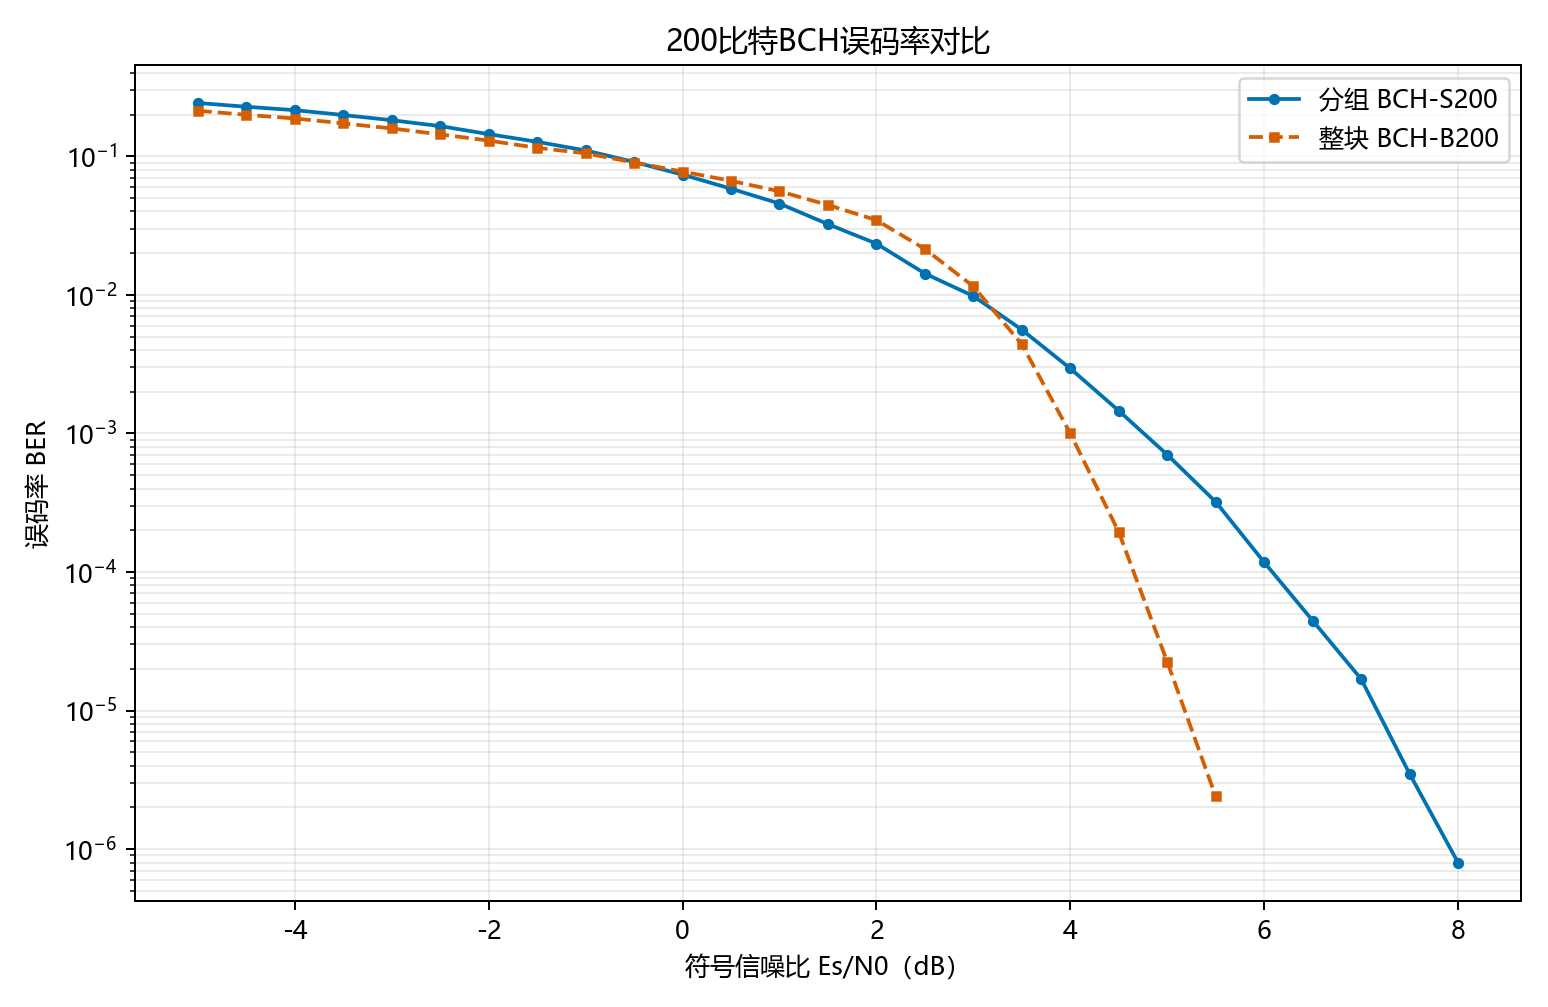
\includegraphics[width=0.90\linewidth]{../Task/Comparison/S6/results/summary/figures/bch_01_ber/figure.png}\\[-0.2em]
    \small（a）比特错误率
  \end{minipage}\par\medskip
  \begin{minipage}{0.92\textwidth}\centering
    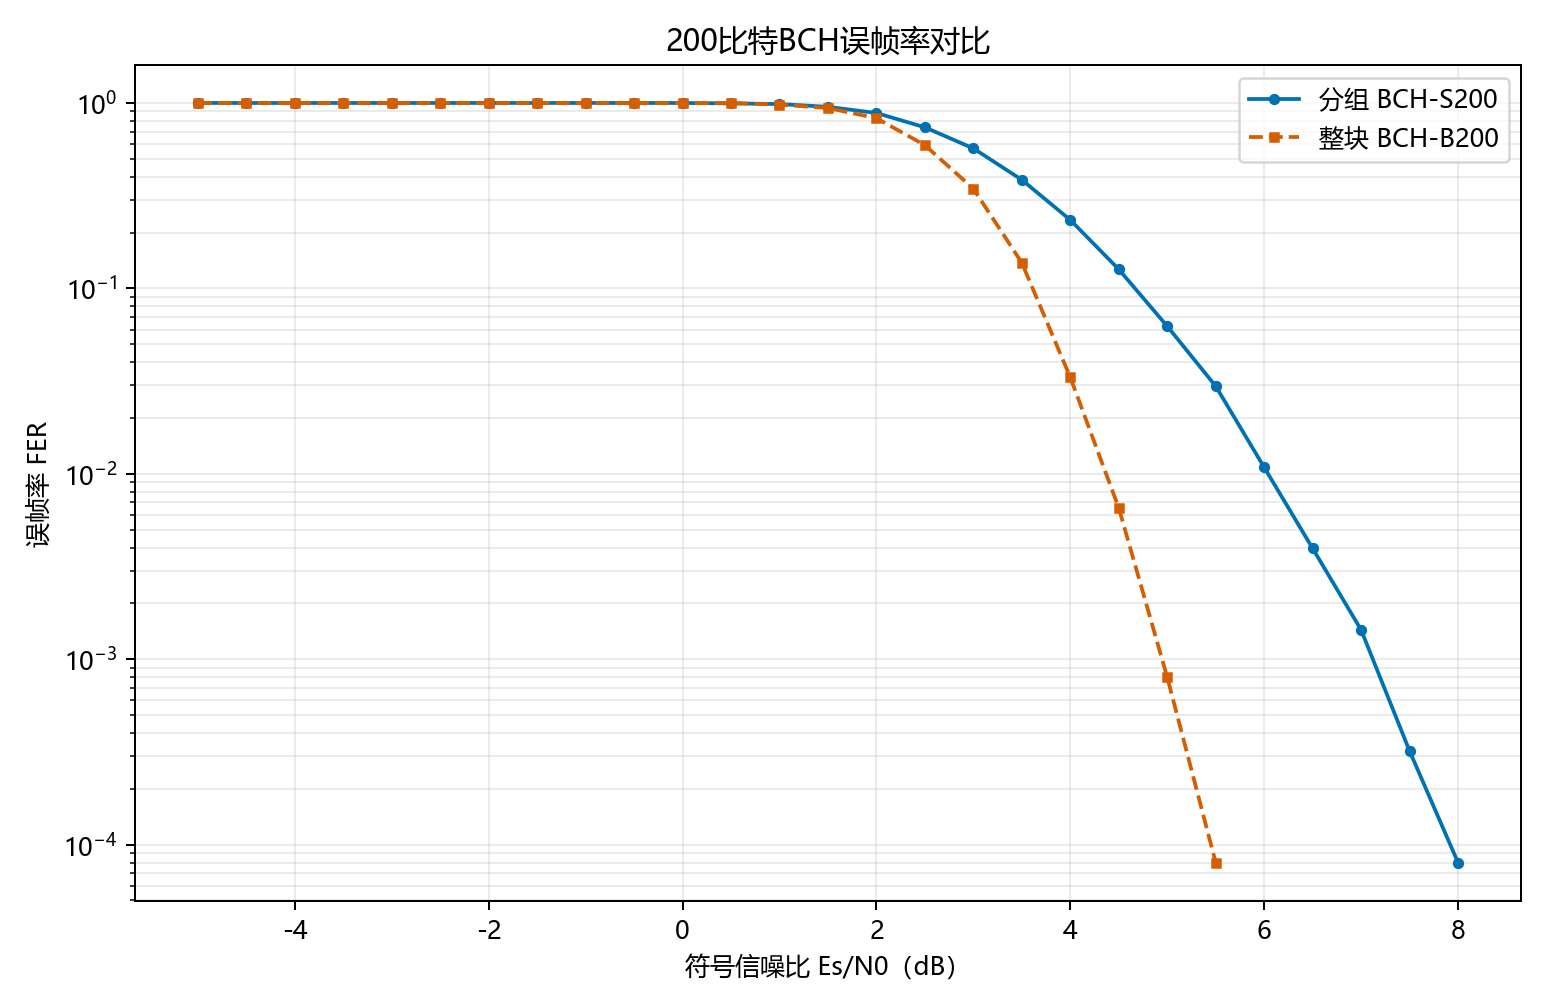
\includegraphics[width=0.90\linewidth]{../Task/Comparison/S6/results/summary/figures/bch_02_fer/figure.png}\\[-0.2em]
    \small（b）帧错误率
  \end{minipage}
  \caption{BCH两类实现的BER与FER}
  \label{fig:s6-bch-reliability}
\end{figure}

\subsection{计算结构与操作统计}

BCH-S200对19个短子块计算综合征；综合征非零时执行位测试、查表、候选比特翻转和译后检查。图\ref{fig:s6-bch-operations}显示，其网格均值为每帧26.92次综合征计算、296.16次综合征位测试和7.92次查表；后三类纠错相关操作会随信道改善而减少。BCH-B200每帧固定完成3060次综合征求值，随后执行BM迭代和Chien位置测试，网格均值分别为8.64次和183.07次，同时伴随约4117.52次有限域加法、1143.42次有限域乘法和3.64次有限域除法。该结构解释了整块方案更重的有限域计算负担，但这些事件不是等价指令，不能用计数总和直接换算处理器周期。

\begin{figure}[p]
  \centering
  \begin{minipage}{0.92\textwidth}\centering
    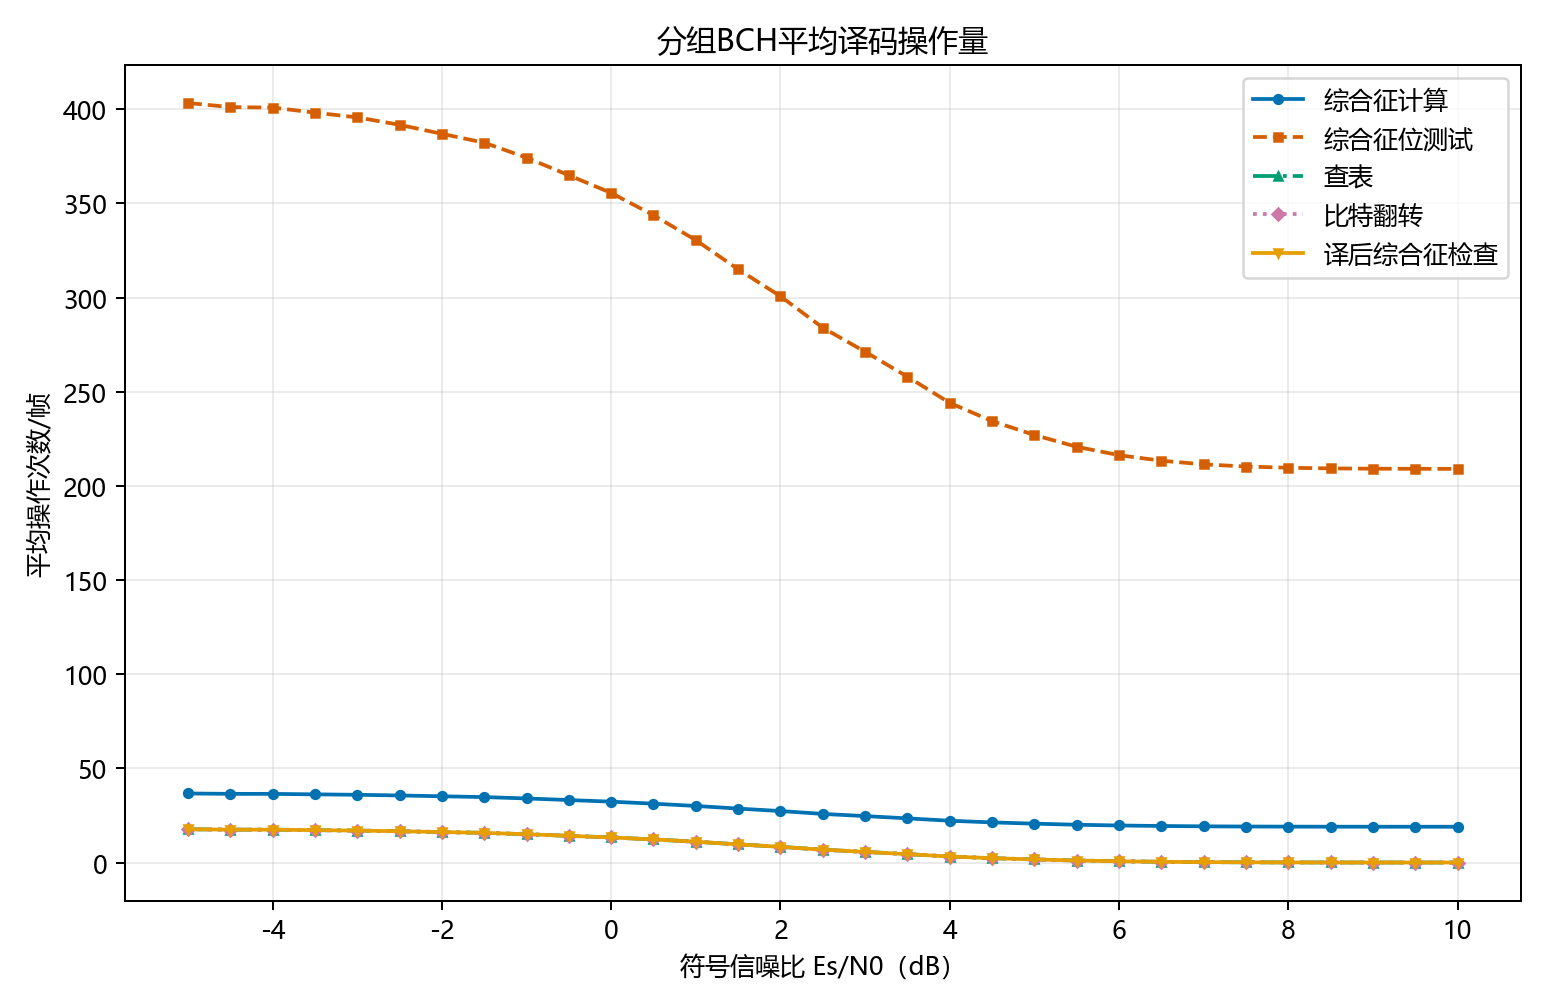
\includegraphics[width=0.72\linewidth]{../Task/Comparison/S6/results/summary/figures/bch_03_segmented_operations/figure.png}\\[-0.2em]
    \small（a）分组查表译码操作
  \end{minipage}\par\medskip
  \begin{minipage}{0.92\textwidth}\centering
    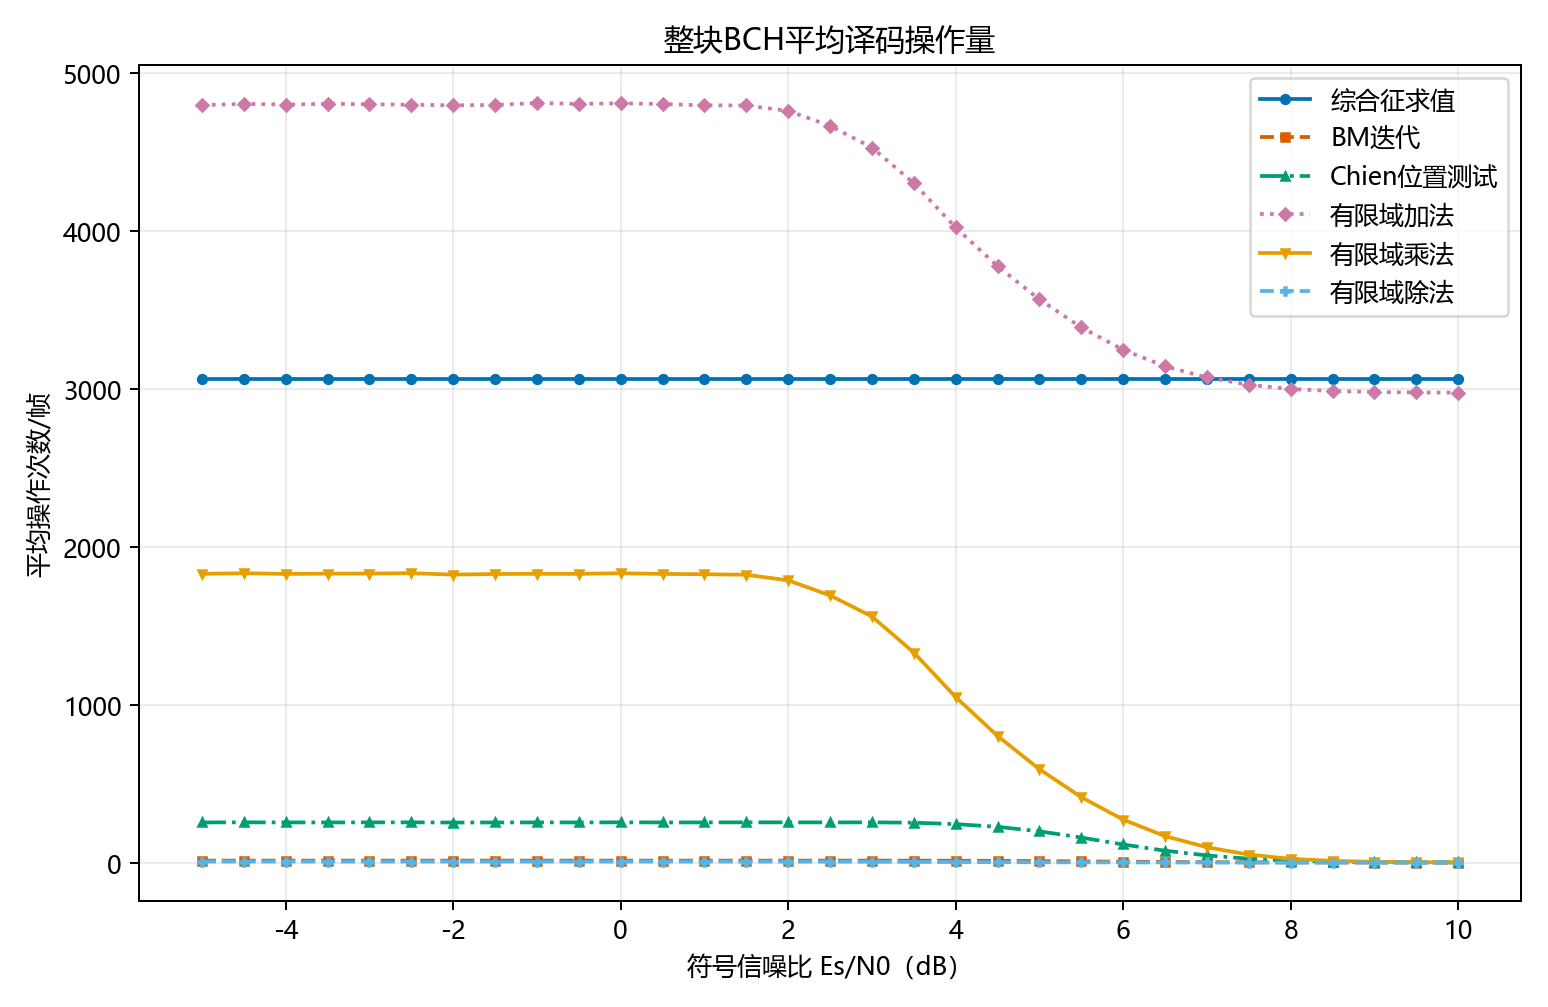
\includegraphics[width=0.72\linewidth]{../Task/Comparison/S6/results/summary/figures/bch_04_block_operations/figure.png}\\[-0.2em]
    \small（b）整块代数译码操作
  \end{minipage}\par\medskip
  \begin{minipage}{0.92\textwidth}\centering
    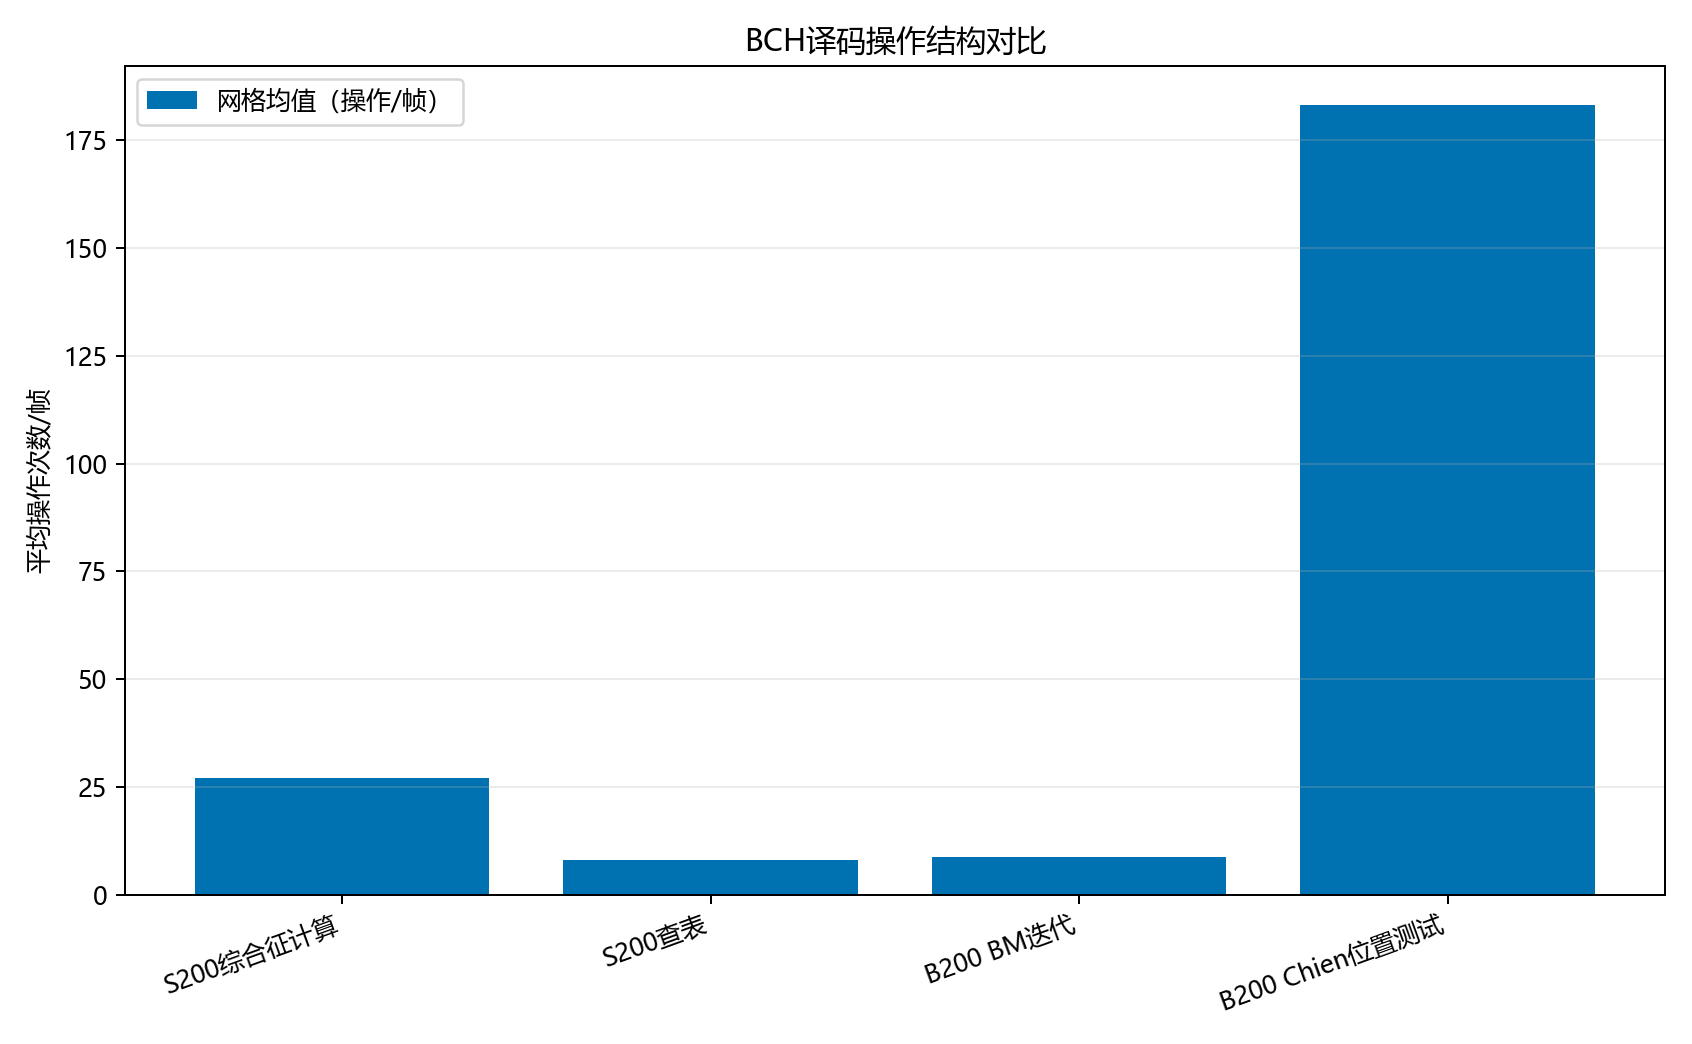
\includegraphics[width=0.68\linewidth]{../Task/Comparison/S6/results/summary/figures/bch_05_operation_structure/figure.png}\\[-0.2em]
    \small（c）主要操作结构的网格均值
  \end{minipage}
  \caption{BCH译码计算结构与操作统计}
  \label{fig:s6-bch-operations}
\end{figure}

\subsection{存储与软件译码时间}

图\ref{fig:s6-bch-memory}中的译码器内存由静态表、对象、输入输出缓冲和工作区按类型与数量建模。BCH-S200总内存为1580 byte，峰值工作区779 byte；BCH-B200总内存为2408 byte，峰值工作区810 byte。整块方案总内存增加828 byte，即52.4\%，主要来自有限域表和代数译码状态；峰值工作区仅增加31 byte。该口径不包含完整进程驻留内存，静态表与临时工作区也未混为同一概念。

\begin{figure}[htbp]
  \centering
  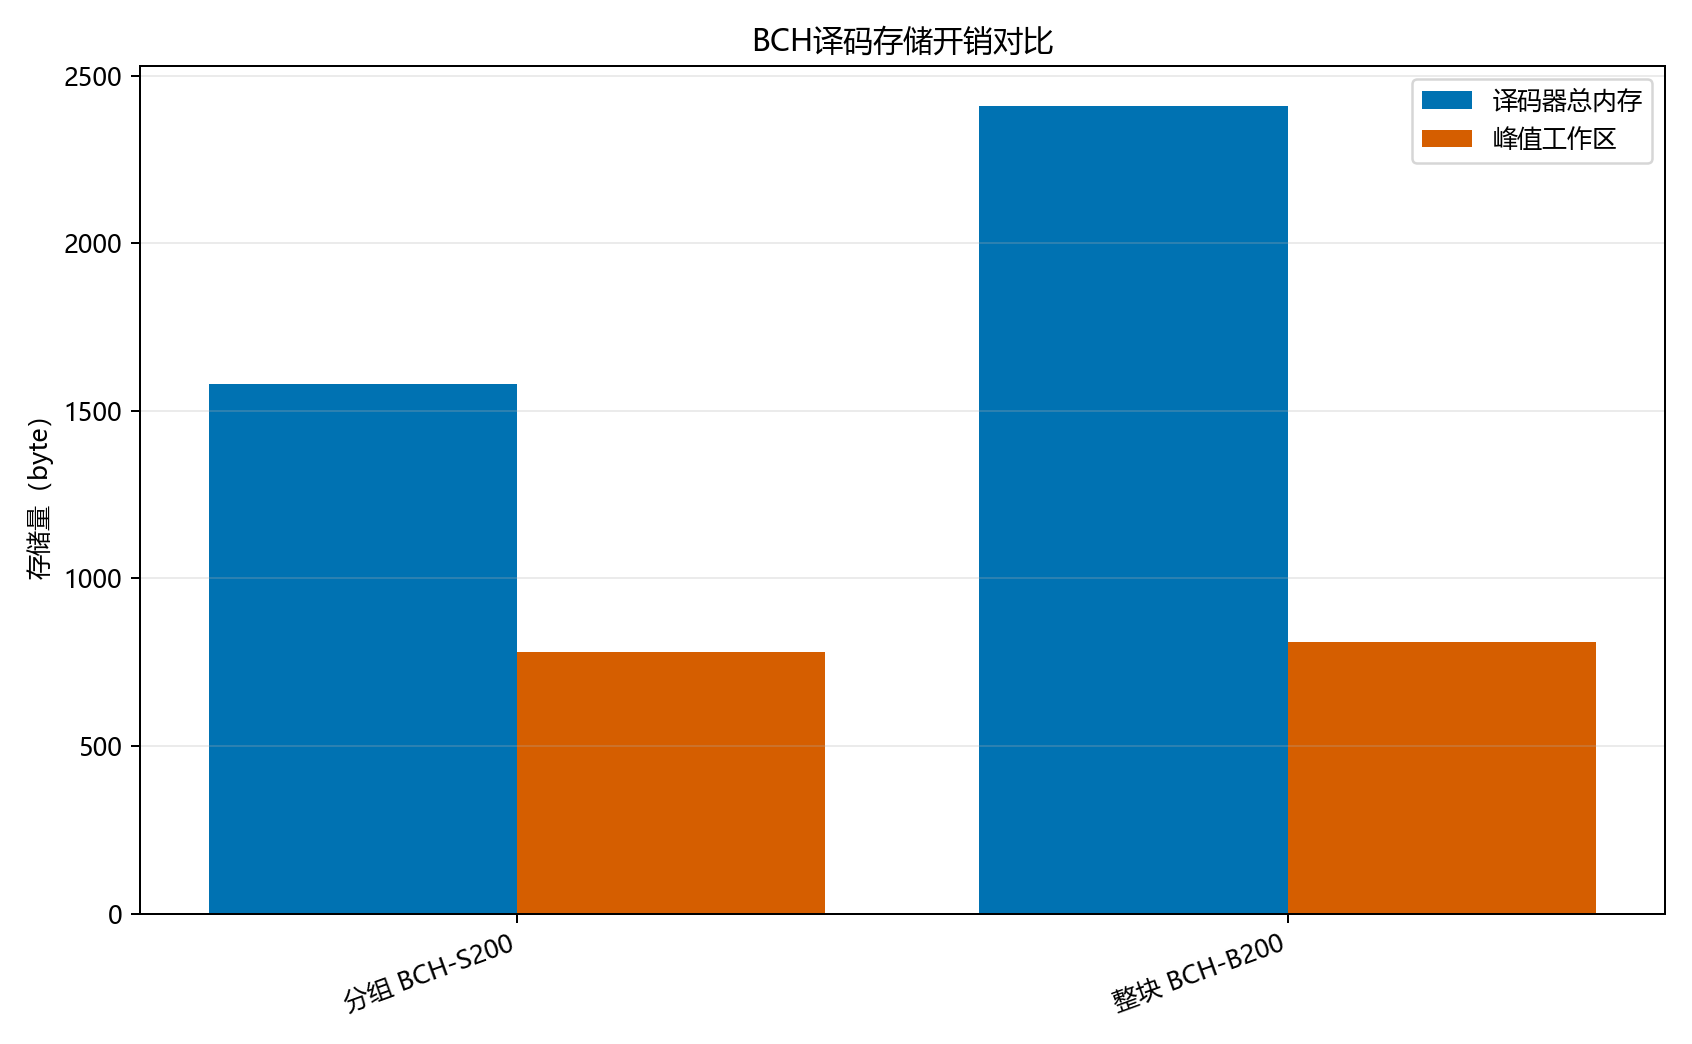
\includegraphics[width=0.90\textwidth]{../Task/Comparison/S6/results/summary/figures/bch_06_memory/figure.png}
  \caption{BCH译码器存储开销}
  \label{fig:s6-bch-memory}
\end{figure}

图\ref{fig:s6-bch-time}覆盖平均、P95、P99和最大观测软件译码时间。按全部信噪比点的帧数加权，S200与B200的平均译码时间分别为10.217~$\mu$s和17.415~$\mu$s，整块方案增加70.5\%；最大观测值分别为25240.3~$\mu$s和27491.4~$\mu$s，增加8.9\%。逐点P95范围分别为10.90--26.53~$\mu$s和15.40--33.52~$\mu$s。P95和P99来自对应正式图数据，而不是不含这两列的汇总表。最大观测值受操作系统调度等影响，只能用于描述当前测量中的尖峰，不能解释为硬实时上界。

\begin{figure}[p]
  \centering
  \begin{minipage}{0.49\textwidth}\centering
    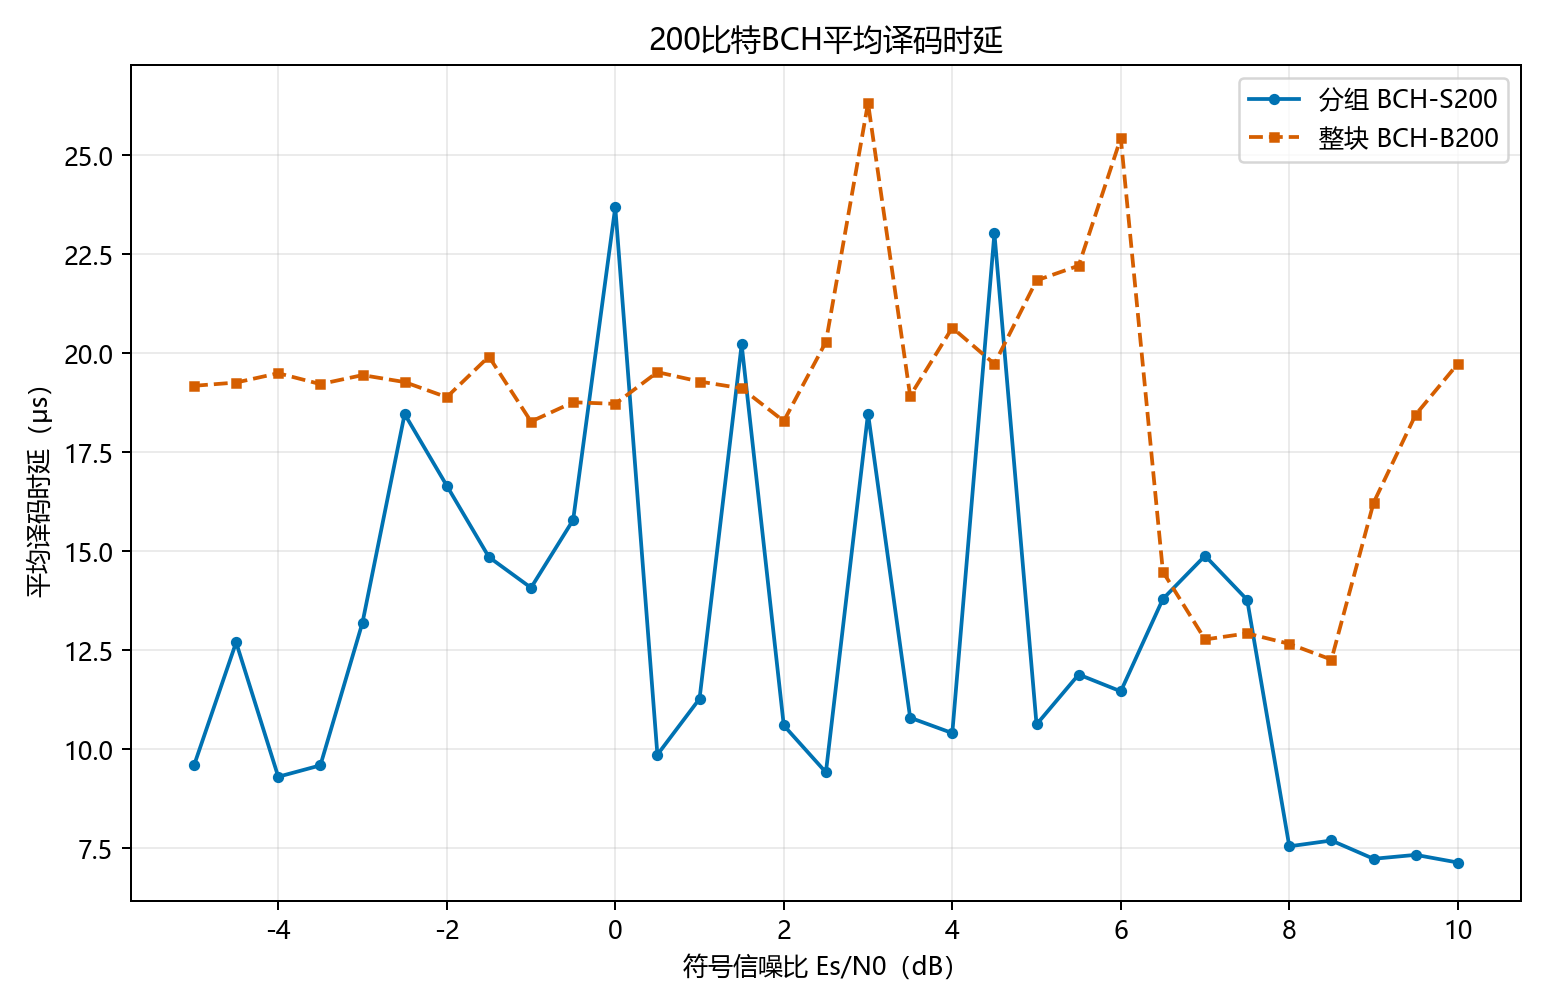
\includegraphics[width=0.98\linewidth]{../Task/Comparison/S6/results/summary/figures/bch_07_avg_time/figure.png}\\[-0.2em]\small（a）平均时间
  \end{minipage}\hfill
  \begin{minipage}{0.49\textwidth}\centering
    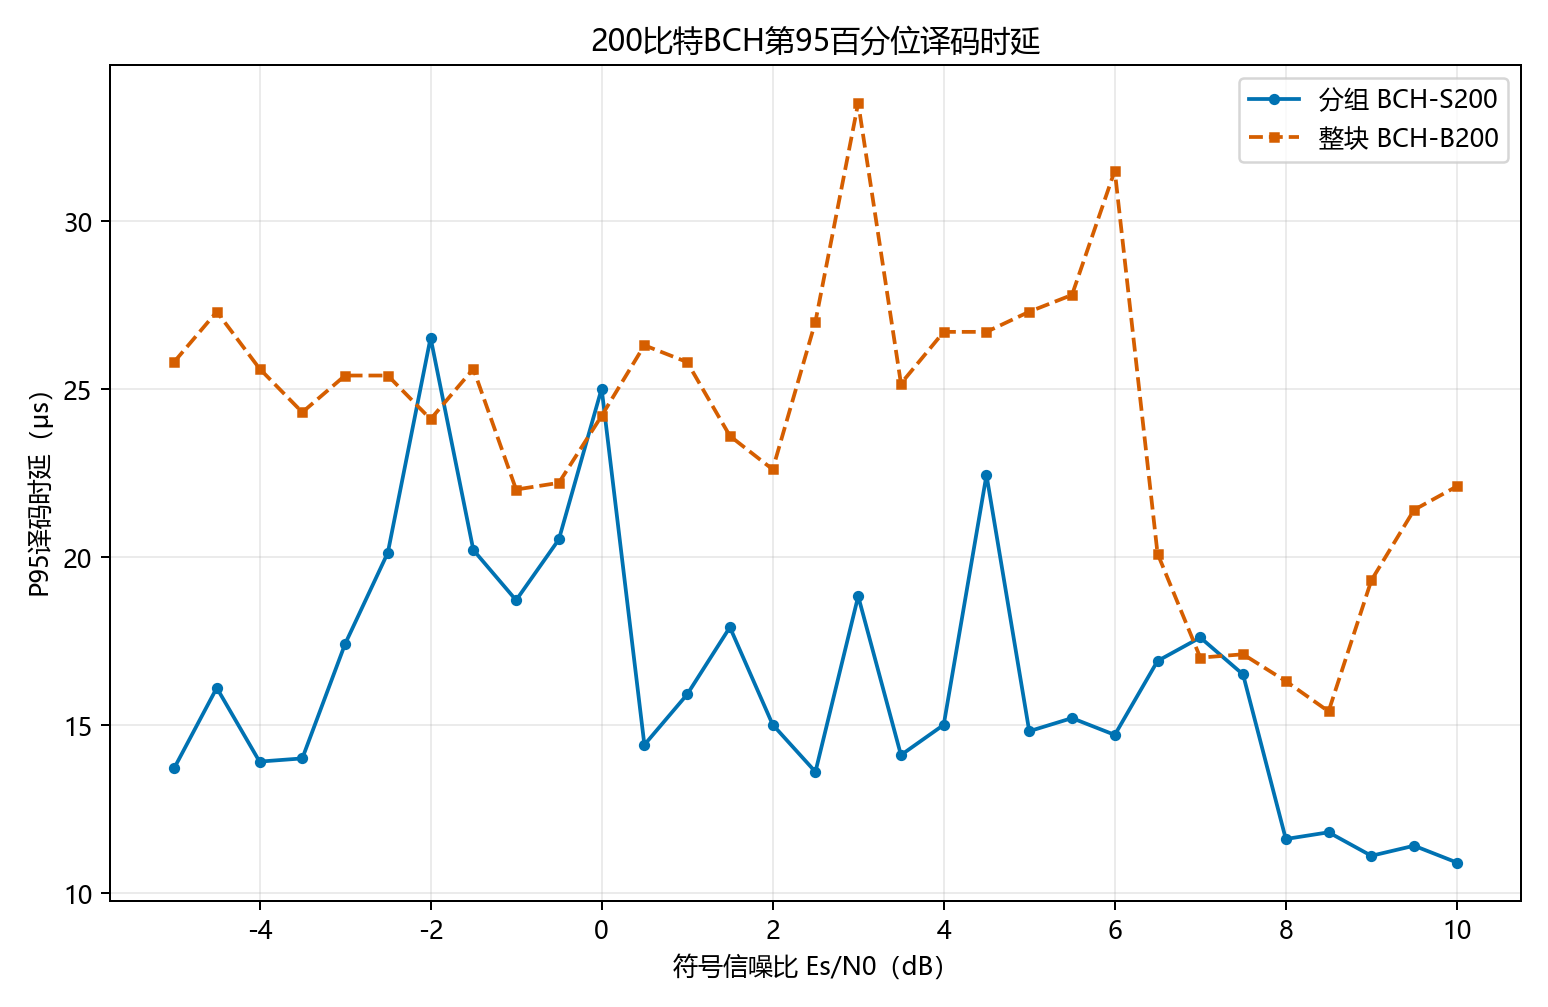
\includegraphics[width=0.98\linewidth]{../Task/Comparison/S6/results/summary/figures/bch_08_p95_time/figure.png}\\[-0.2em]\small（b）P95时间
  \end{minipage}\par\medskip
  \begin{minipage}{0.49\textwidth}\centering
    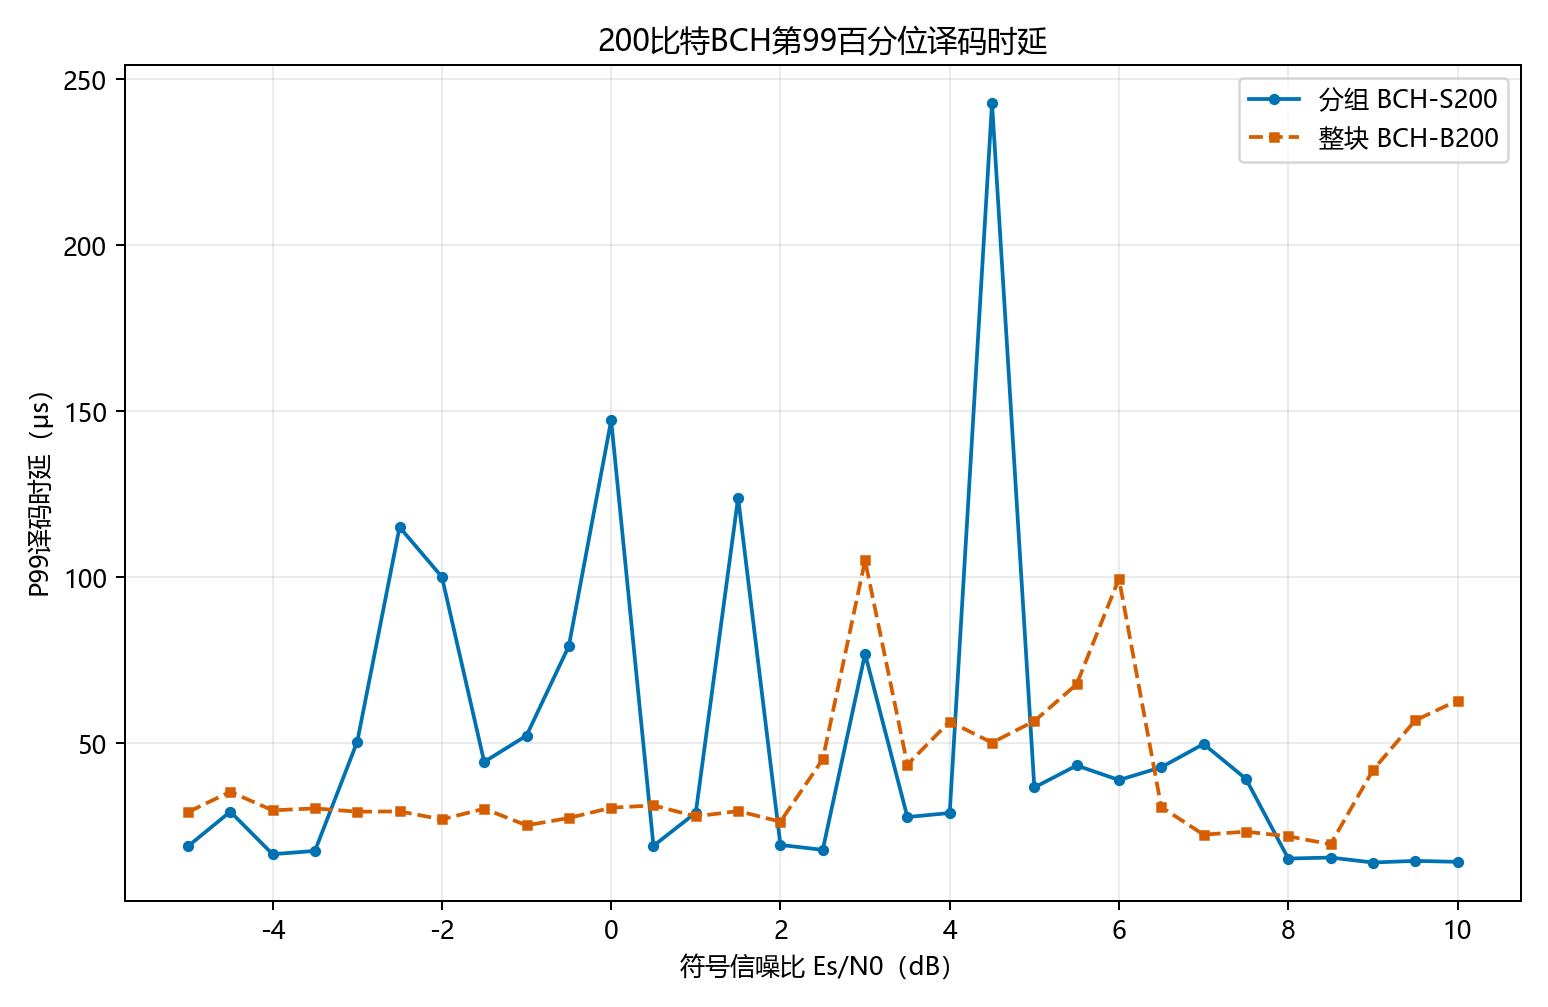
\includegraphics[width=0.98\linewidth]{../Task/Comparison/S6/results/summary/figures/bch_09_p99_time/figure.png}\\[-0.2em]\small（c）P99时间
  \end{minipage}\hfill
  \begin{minipage}{0.49\textwidth}\centering
    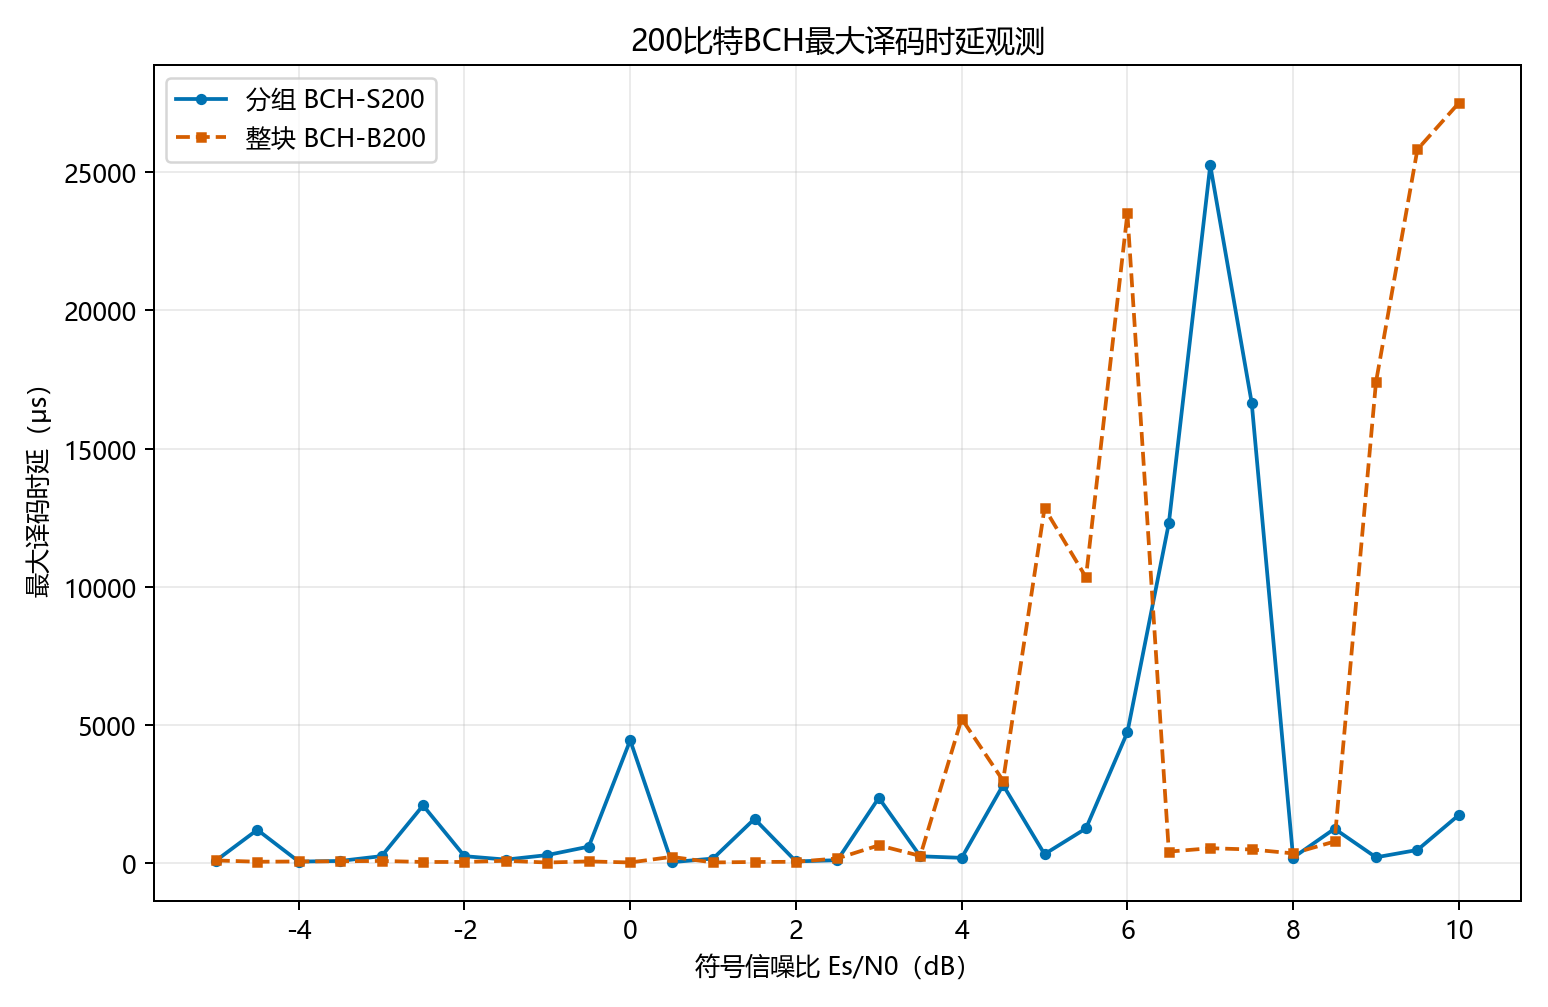
\includegraphics[width=0.98\linewidth]{../Task/Comparison/S6/results/summary/figures/bch_10_max_time/figure.png}\\[-0.2em]\small（d）最大观测时间
  \end{minipage}
  \caption{BCH译码时间统计}
  \label{fig:s6-bch-time}
\end{figure}

\begin{table}[htbp]
  \centering
  \scriptsize
  \caption{BCH可靠性、资源与软件时间汇总}
  \label{tab:s6-bch-summary}
  \setlength{\tabcolsep}{2.1pt}
  \begin{tabular}{p{0.12\textwidth}ccccc p{0.20\textwidth}}
    \toprule
    方案 & FER=0.1/dB & FER=0.01/dB & 加权平均/$\mu$s & 最大观测/$\mu$s & 内存/byte & 主要计算结构 \\
    \midrule
    BCH-S200 & 4.667 & 6.040 & 10.217 & 25240.3 & 1580 & 19组综合征、查表、翻转和译后检查 \\
    BCH-B200 & 3.612 & 4.369 & 17.415 & 27491.4 & 2408 & 综合征、BM、Chien及有限域运算 \\
    \bottomrule
  \end{tabular}
\end{table}

\subsection{BCH工程结论}

在本项目既定实现中，BCH-S200的短分组、固定查表和较小工作区形成了更低的软件时间与更简单的实现结构，适合资源受限且允许较高链路信噪比的场景。BCH-B200以BM、Chien搜索和有限域表开销换取整块$t=6$纠错能力，在FER为0.01时比S200节省1.671 dB，同时平均软件译码时间增加约70.5\%、模型内存增加52.4\%。该权衡属于完整编码组织和译码结构共同变化的结果，不应归因于单一译码算法。

\section{卷积码硬判决与软判决Viterbi对比}

\subsection{正式配置与判决定义}

卷积码使用300 bit载荷和6个终止比特，$R=1/2$不打孔，实际发送612 bit，实际码率为0.4902。整块方案一次处理306个网格输入步，$D=W=306$、$S=300$；连续方案按50$\times$6、100$\times$3和150$\times$2三种业务组织输入，均使用回溯深度$D=70$、窗口长度$W=128$和滑动步长$S=25$。硬判决把接收样值阈值化为0/1比特，以汉明距离构造分支度量；浮点软判决保留连续BPSK接收符号，以接收符号与理想$\pm1$符号之间的欧氏距离平方构造分支度量，并非LLR输入。

卷积码证据复用S3 Stage14的正式仿真数据并在S6中统一整理，S6没有按相同停止时刻重新执行逐帧strict pair-stop。因此，本节依据相同配置、信噪比网格和正式统计曲线比较硬、软判决差异，不进行逐帧差分因果推断。该限制不否定已有统计结果，但限定了结论的精度和表达范围。

\subsection{BER、FER与门限差异}

图\ref{fig:s6-cc-reliability}显示，整块和三种连续组织下，浮点软判决均比硬判决更早进入低错误率区。整块方案在FER为0.1时，软、硬判决门限分别为$-0.731$ dB和1.367 dB，软判决节省2.098 dB；在FER为0.01时，两者分别为0.229 dB和2.489 dB，差值为2.260 dB。三种连续组织的FER曲线及门限与整块统计一致，说明在当前终止、窗口和输出组织下，可靠性差异主要由判决信息精度决定，而组织方式主要改变执行与输出时序。

\begin{figure}[p]
  \centering
  \begin{minipage}{0.92\textwidth}\centering
    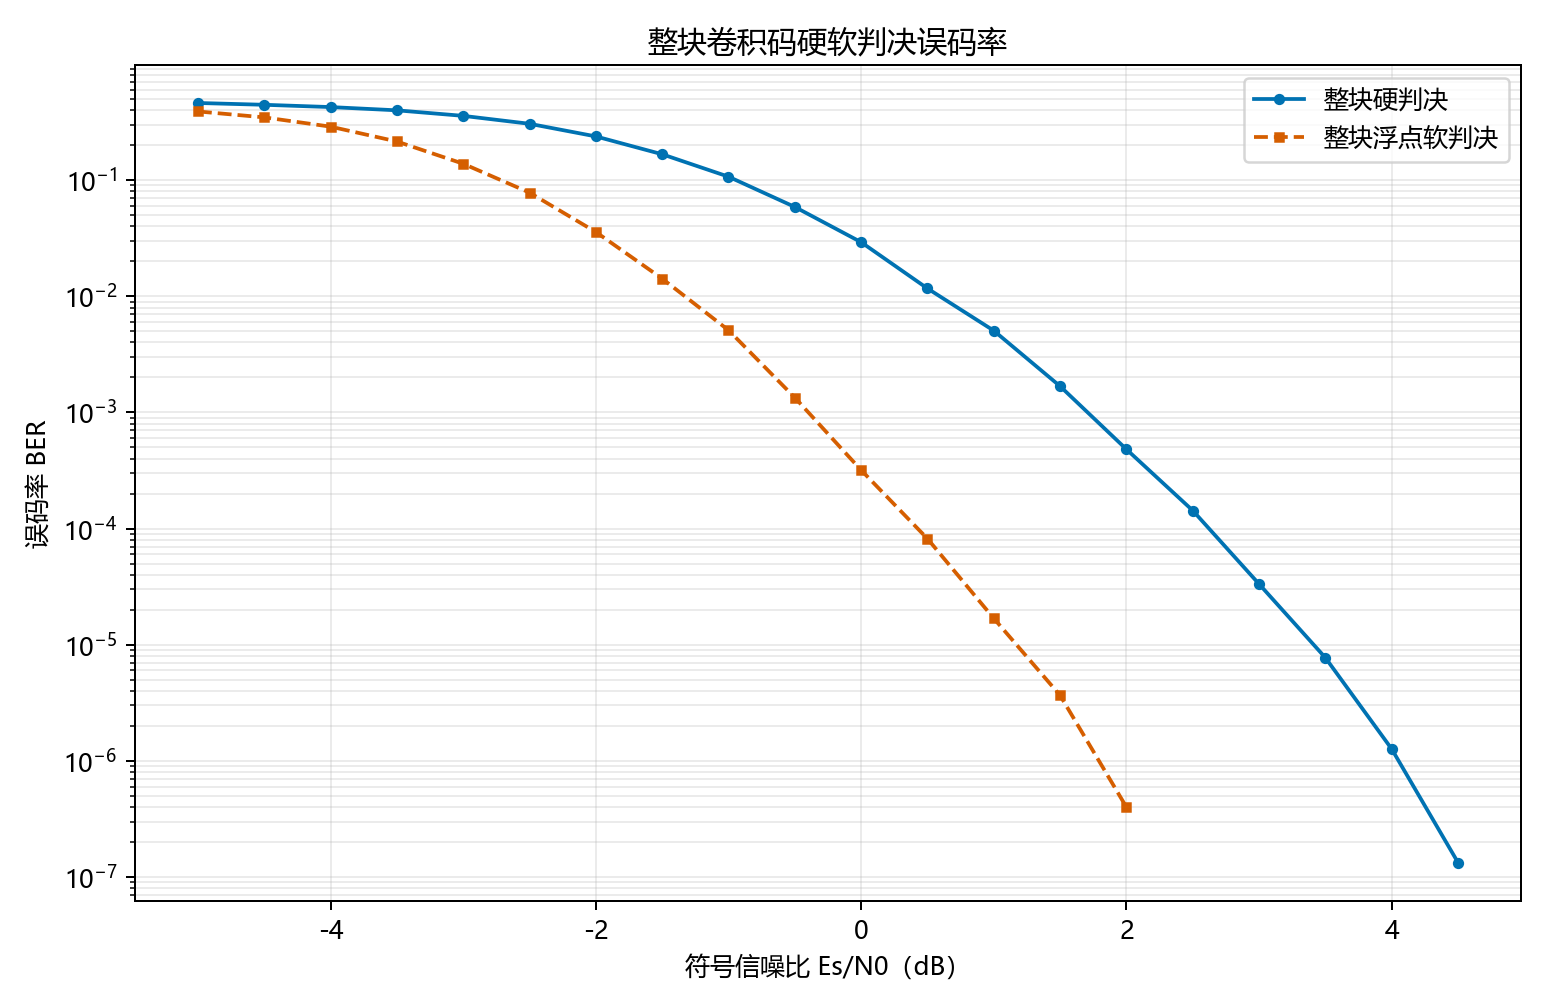
\includegraphics[width=0.70\linewidth]{../Task/Comparison/S6/results/summary/figures/cc_01_block_ber/figure.png}\\[-0.2em]\small（a）整块译码BER
  \end{minipage}\par\medskip
  \begin{minipage}{0.92\textwidth}\centering
    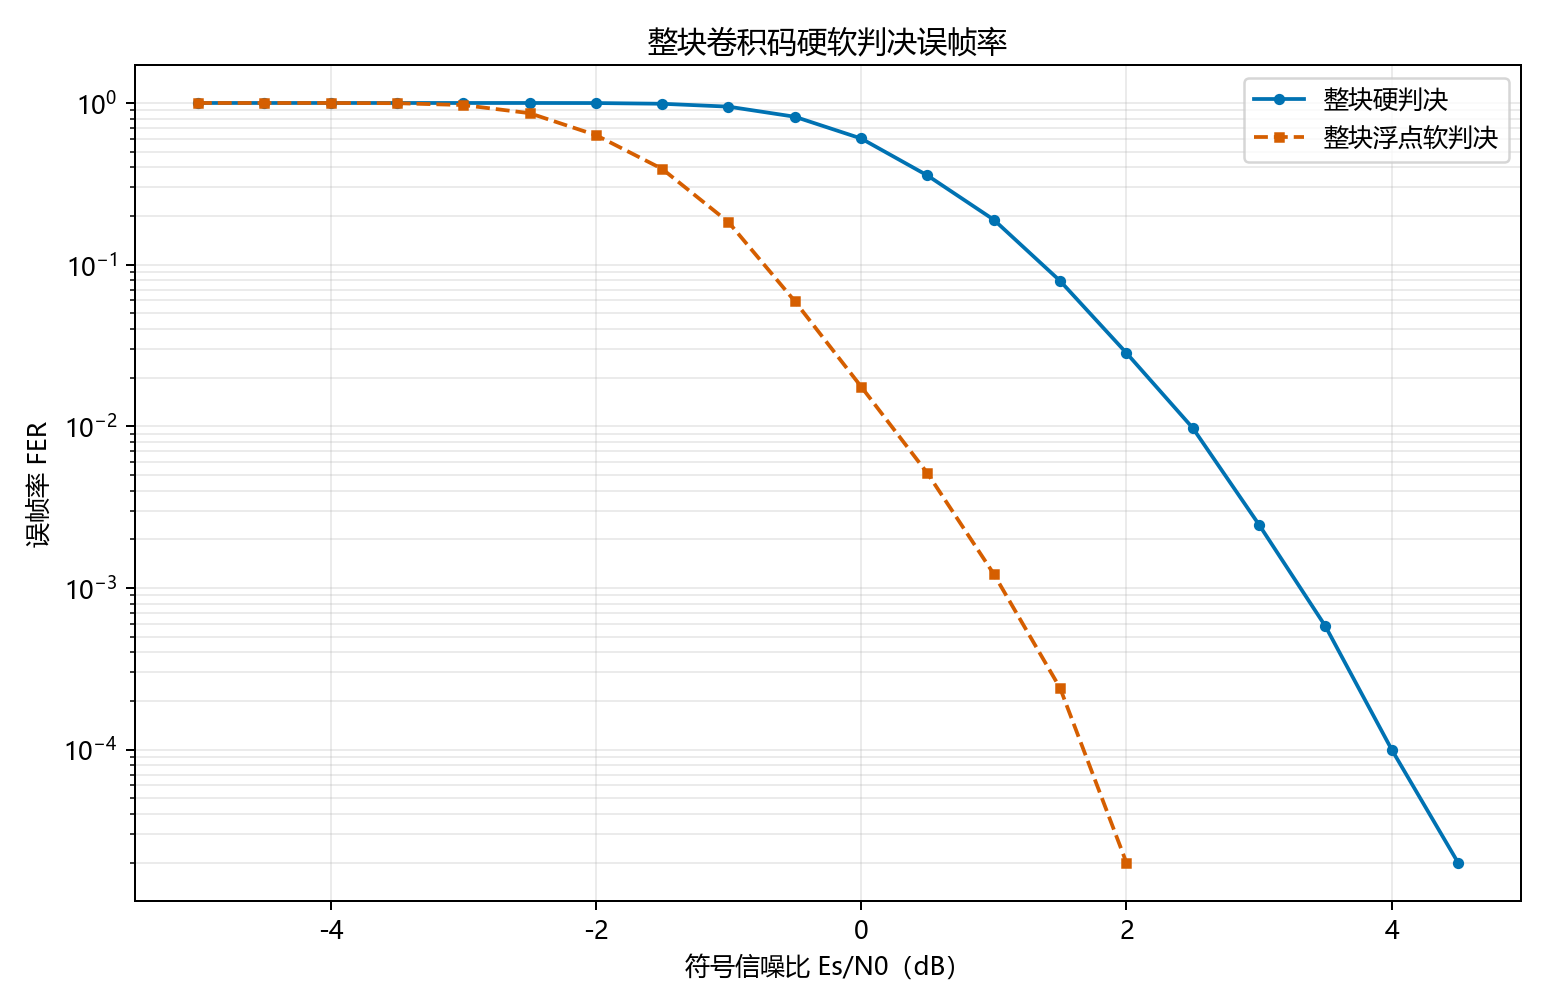
\includegraphics[width=0.70\linewidth]{../Task/Comparison/S6/results/summary/figures/cc_02_block_fer/figure.png}\\[-0.2em]\small（b）整块译码FER
  \end{minipage}\par\medskip
  \begin{minipage}{0.92\textwidth}\centering
    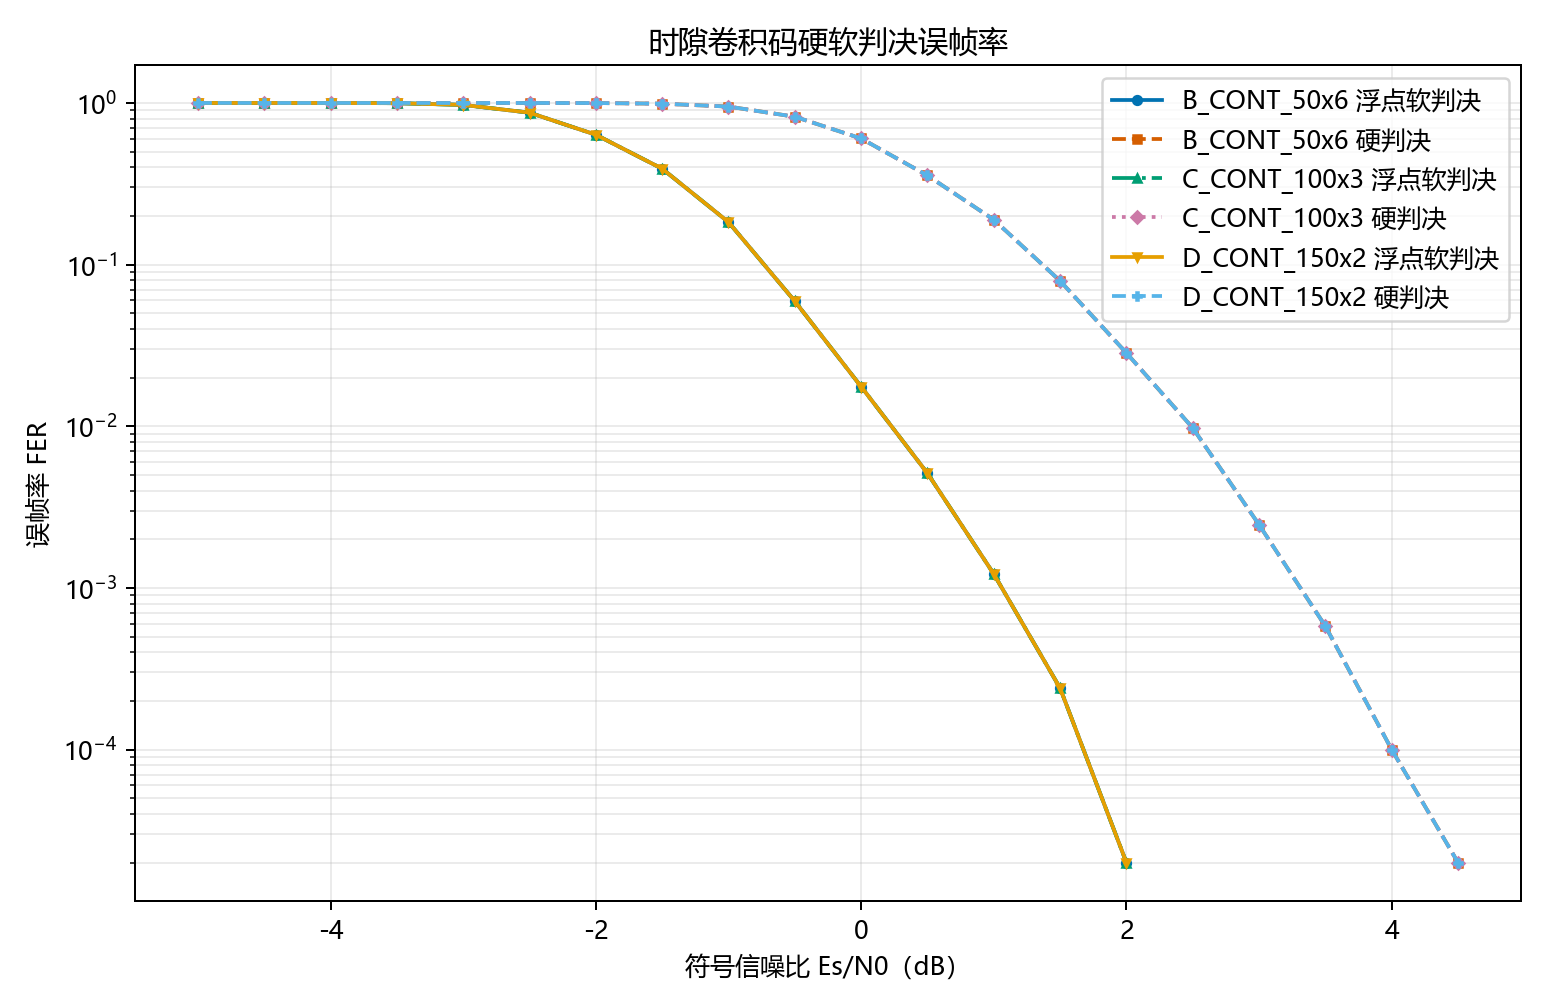
\includegraphics[width=0.70\linewidth]{../Task/Comparison/S6/results/summary/figures/cc_03_slot_fer/figure.png}\\[-0.2em]\small（c）连续组织FER
  \end{minipage}
  \caption{卷积码硬判决与浮点软判决的BER和FER}
  \label{fig:s6-cc-reliability}
\end{figure}

\begin{table}[htbp]
  \centering
  \scriptsize
  \caption{卷积码硬判决与浮点软判决的可靠性门限}
  \label{tab:s6-cc-thresholds}
  \setlength{\tabcolsep}{2.4pt}
  \begin{tabular}{p{0.16\textwidth}p{0.12\textwidth}ccc p{0.18\textwidth}}
    \toprule
    组织方式 & 判决 & FER=0.1/dB & FER=0.01/dB & 相对硬判决增益/dB & 说明 \\
    \midrule
    整块及三种连续组织 & 硬判决 & 1.367 & 2.489 & 0 & 1 bit判决，汉明距离分支度量 \\
    整块及三种连续组织 & 浮点软判决 & $-0.731$ & 0.229 & 2.098/2.260 & 连续符号，欧氏距离平方分支度量 \\
    \bottomrule
  \end{tabular}
\end{table}

\subsection{复杂度、存储与软件时间}

硬、软Viterbi采用相同状态数、候选分支数、ACS骨架和回溯骨架，因此图\ref{fig:s6-cc-resource}中同一组织的ACS与回溯计数相同。整块译码每帧39168次ACS和306次回溯操作；连续组织因窗口重复处理，每帧约143998次ACS和866次回溯操作。相同ACS计数不表示总计算代价相同：硬判决分支度量以比特比较和汉明距离为主，浮点软判决需要减法、平方和加法。模型内存由组织方式决定，整块为59776 byte，连续窗口为26112 byte，判决精度在当前内存模型中没有改变这一数值。

\begin{figure}[p]
  \centering
  \begin{minipage}{0.92\textwidth}\centering
    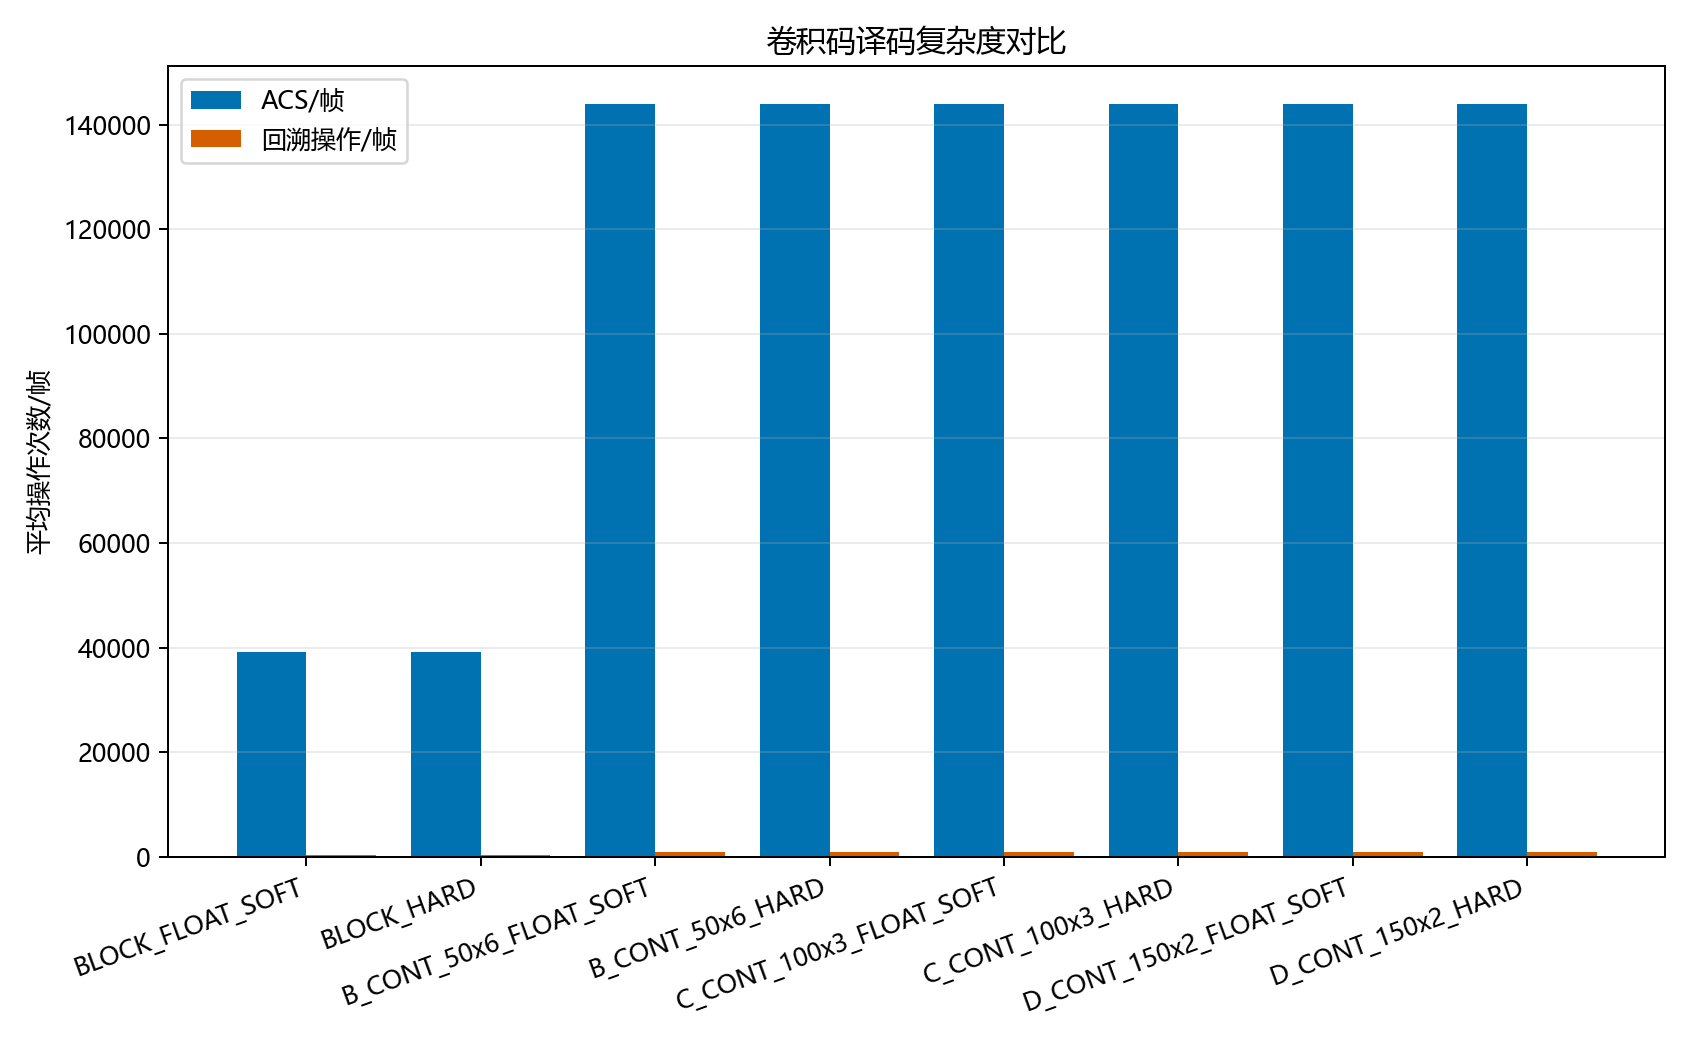
\includegraphics[width=0.90\linewidth]{../Task/Comparison/S6/results/summary/figures/cc_04_complexity/figure.png}\\[-0.2em]\small（a）ACS与回溯操作
  \end{minipage}\par\medskip
  \begin{minipage}{0.92\textwidth}\centering
    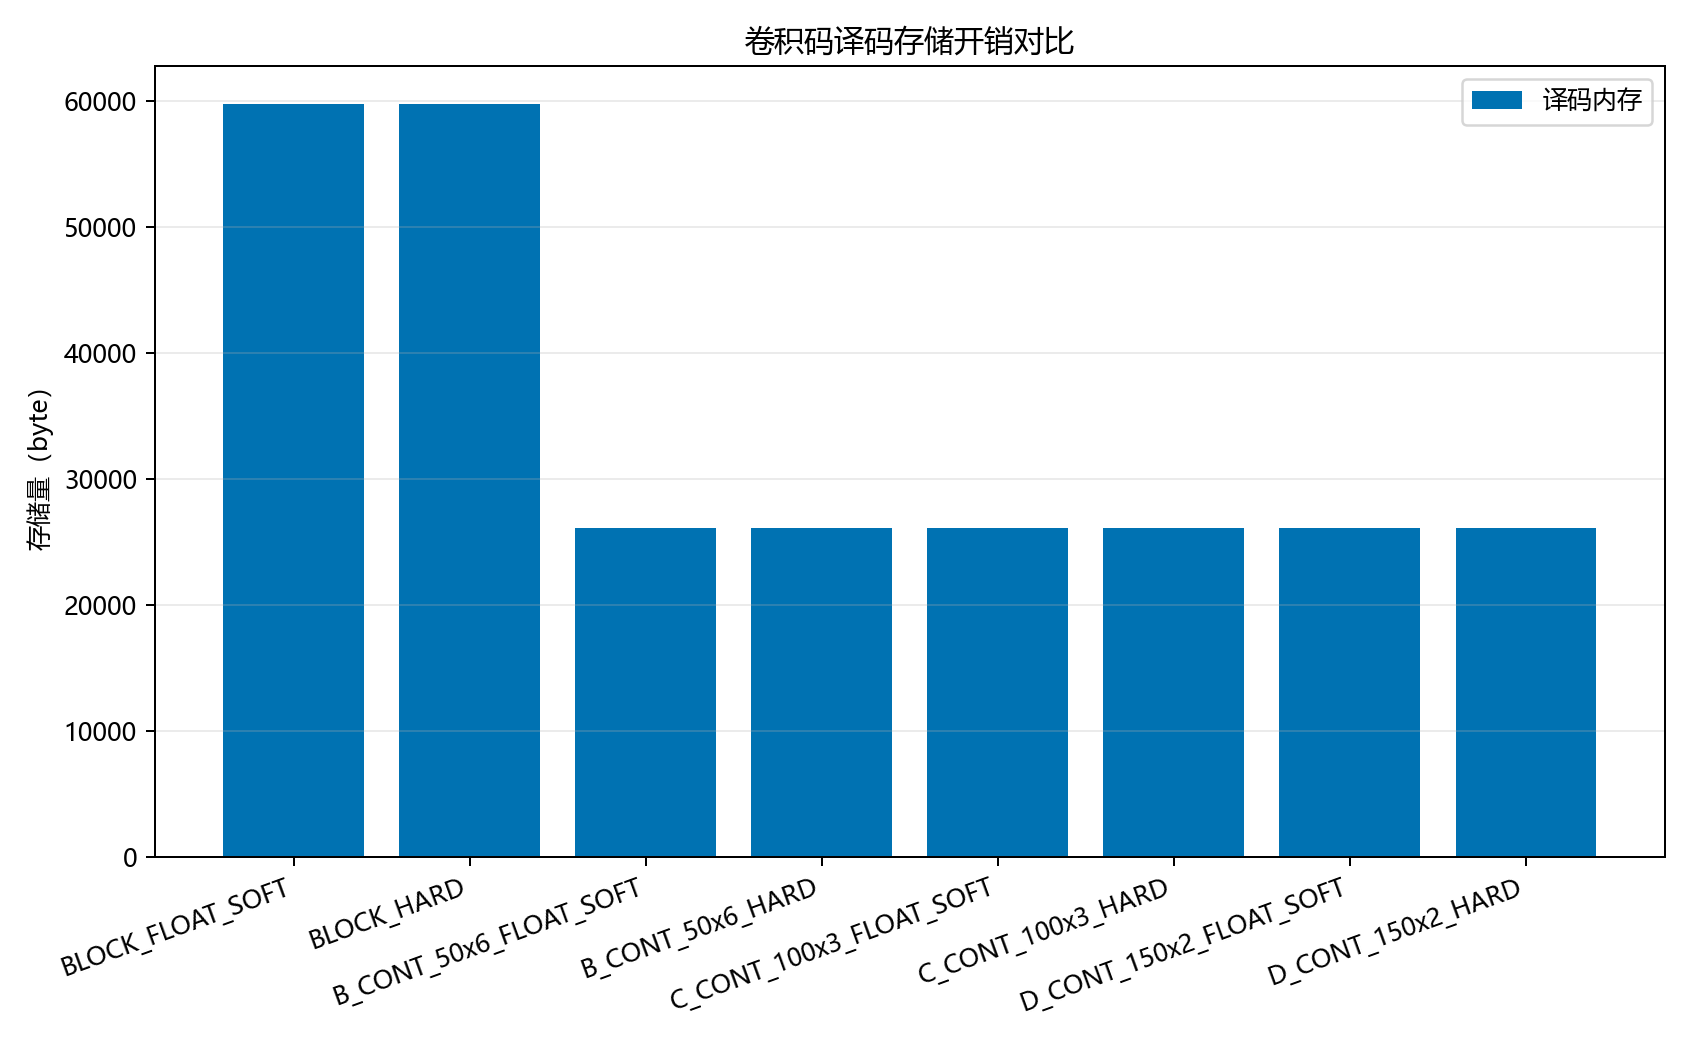
\includegraphics[width=0.90\linewidth]{../Task/Comparison/S6/results/summary/figures/cc_05_memory/figure.png}\\[-0.2em]\small（b）译码器内存
  \end{minipage}
  \caption{卷积码Viterbi译码的操作规模与存储开销}
  \label{fig:s6-cc-resource}
\end{figure}

图\ref{fig:s6-cc-latency}区分CPU软件译码时间、首输出时延和决策时延。整块硬、软判决的帧加权平均译码时间分别为339.03~$\mu$s和524.00~$\mu$s，浮点软判决增加54.6\%；最大观测时间分别为34231.5~$\mu$s和65607.2~$\mu$s。三种连续组织的硬判决加权平均时间为1549.17--1565.58~$\mu$s，软判决为1835.82--1849.69~$\mu$s，增加约18\%。连续组织的首输出时延为298或398个符号，平均决策时延图所示值为342、430或530个符号；二者由到达批次、窗口和回溯调度决定，不能称为平均译码时间或最大译码时间。

\begin{figure}[p]
  \centering
  \begin{minipage}{0.92\textwidth}\centering
    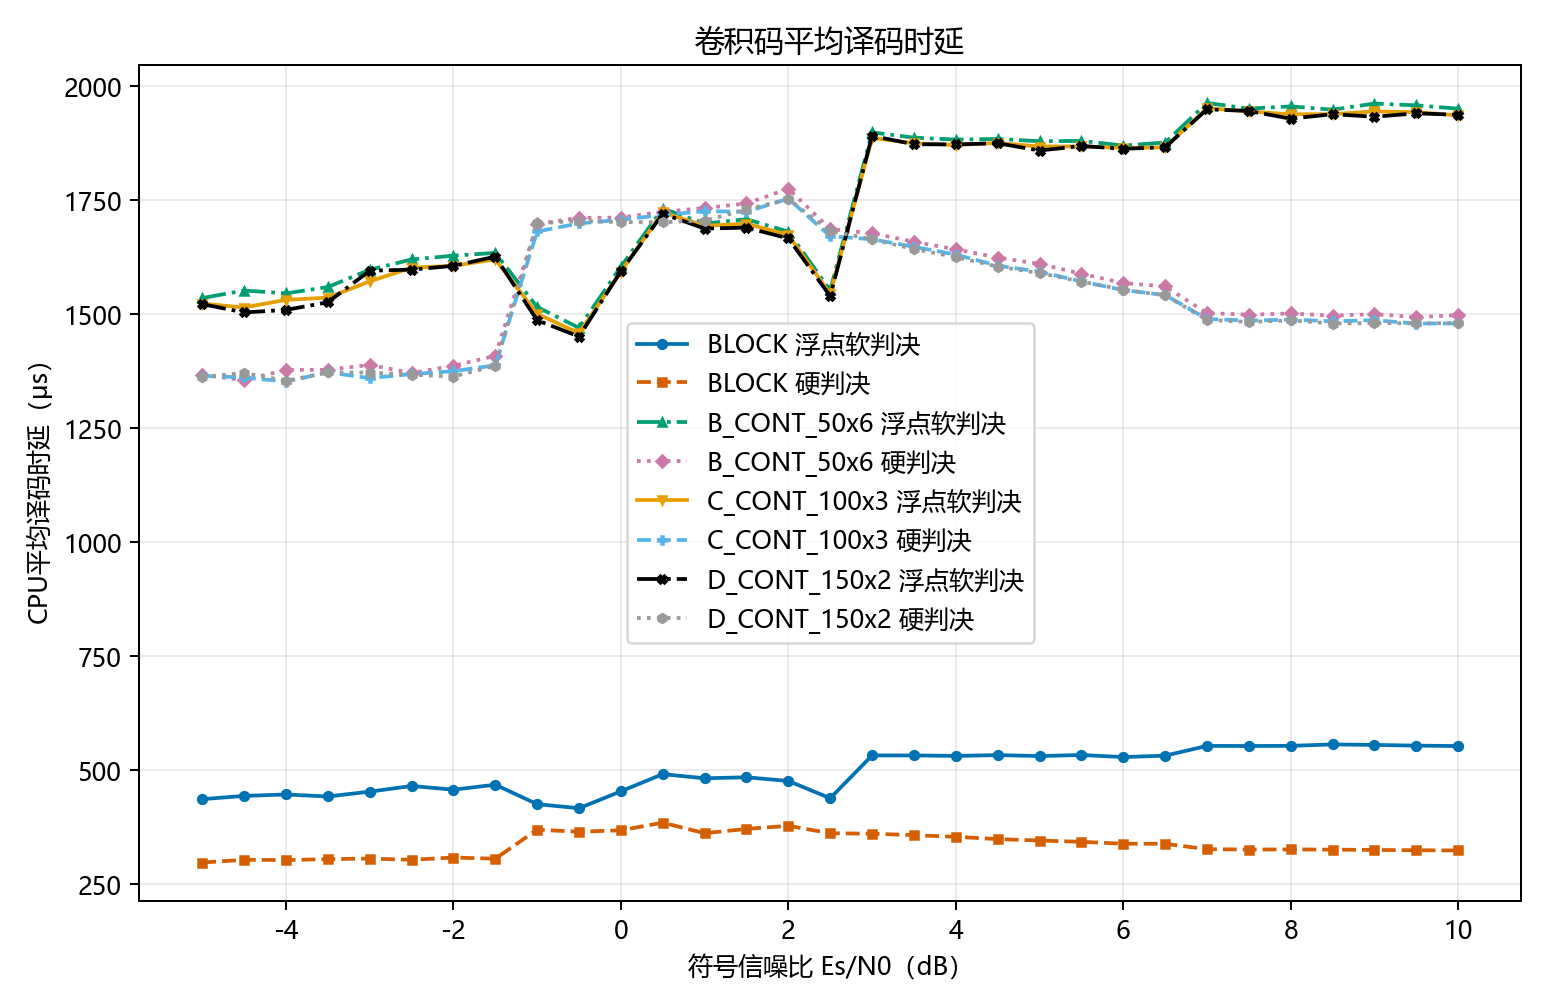
\includegraphics[width=0.90\linewidth]{../Task/Comparison/S6/results/summary/figures/cc_06_avg_time/figure.png}\\[-0.2em]\small（a）平均CPU译码时间
  \end{minipage}\par\medskip
  \begin{minipage}{0.49\textwidth}\centering
    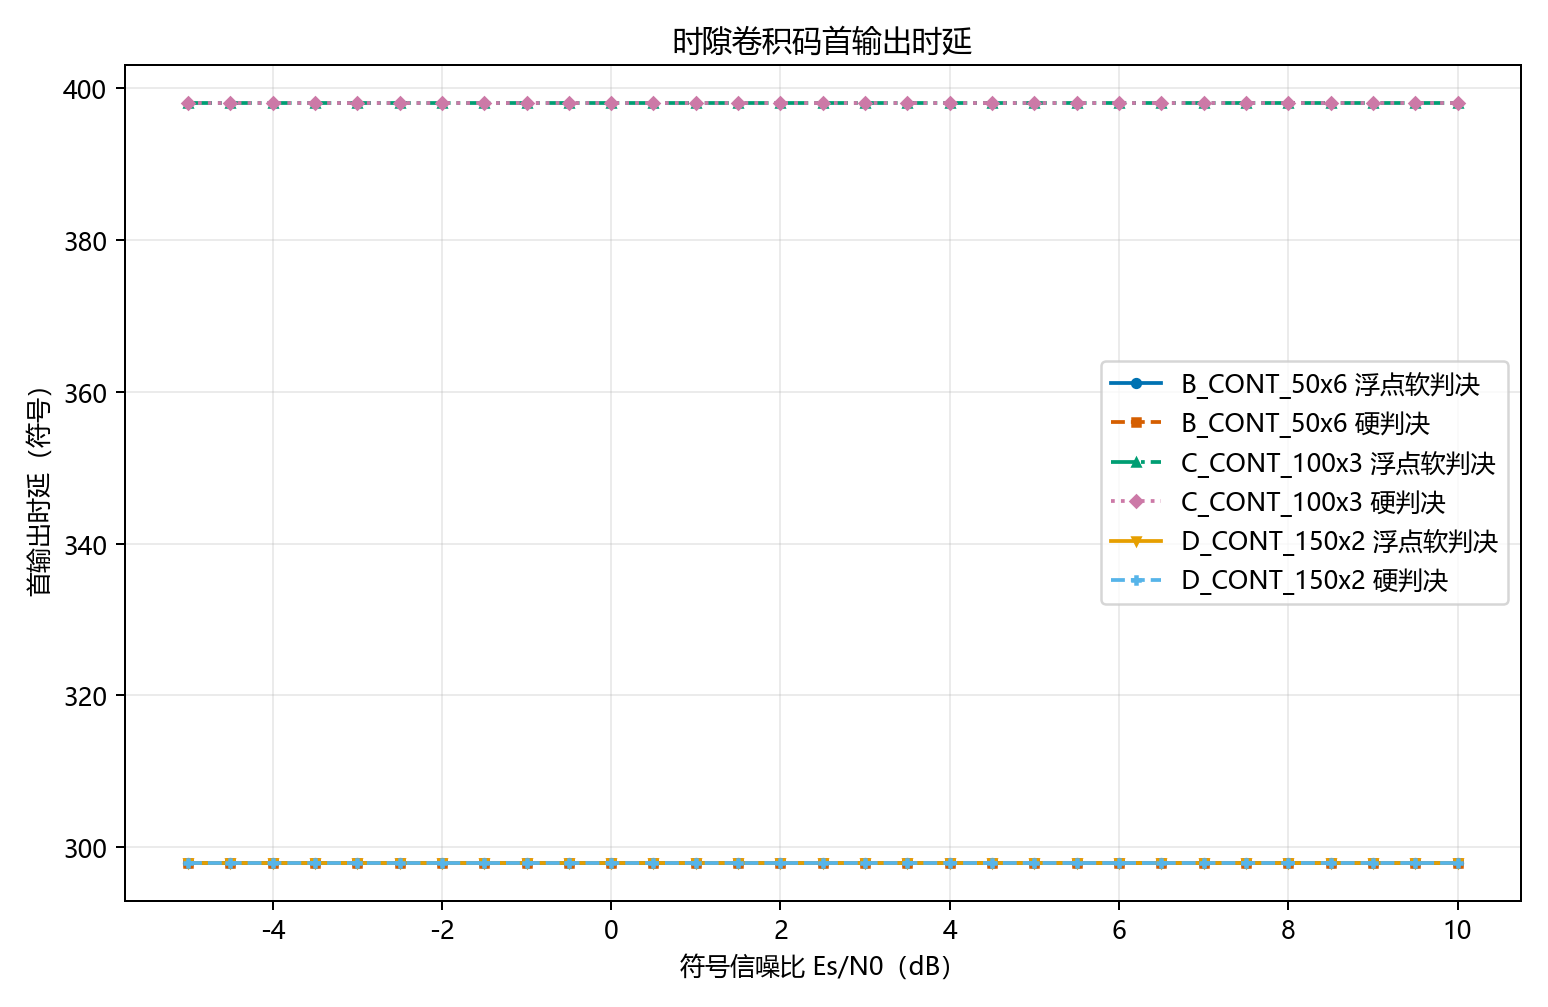
\includegraphics[width=0.98\linewidth]{../Task/Comparison/S6/results/summary/figures/cc_07_first_output/figure.png}\\[-0.2em]\small（b）首输出时延
  \end{minipage}\hfill
  \begin{minipage}{0.49\textwidth}\centering
    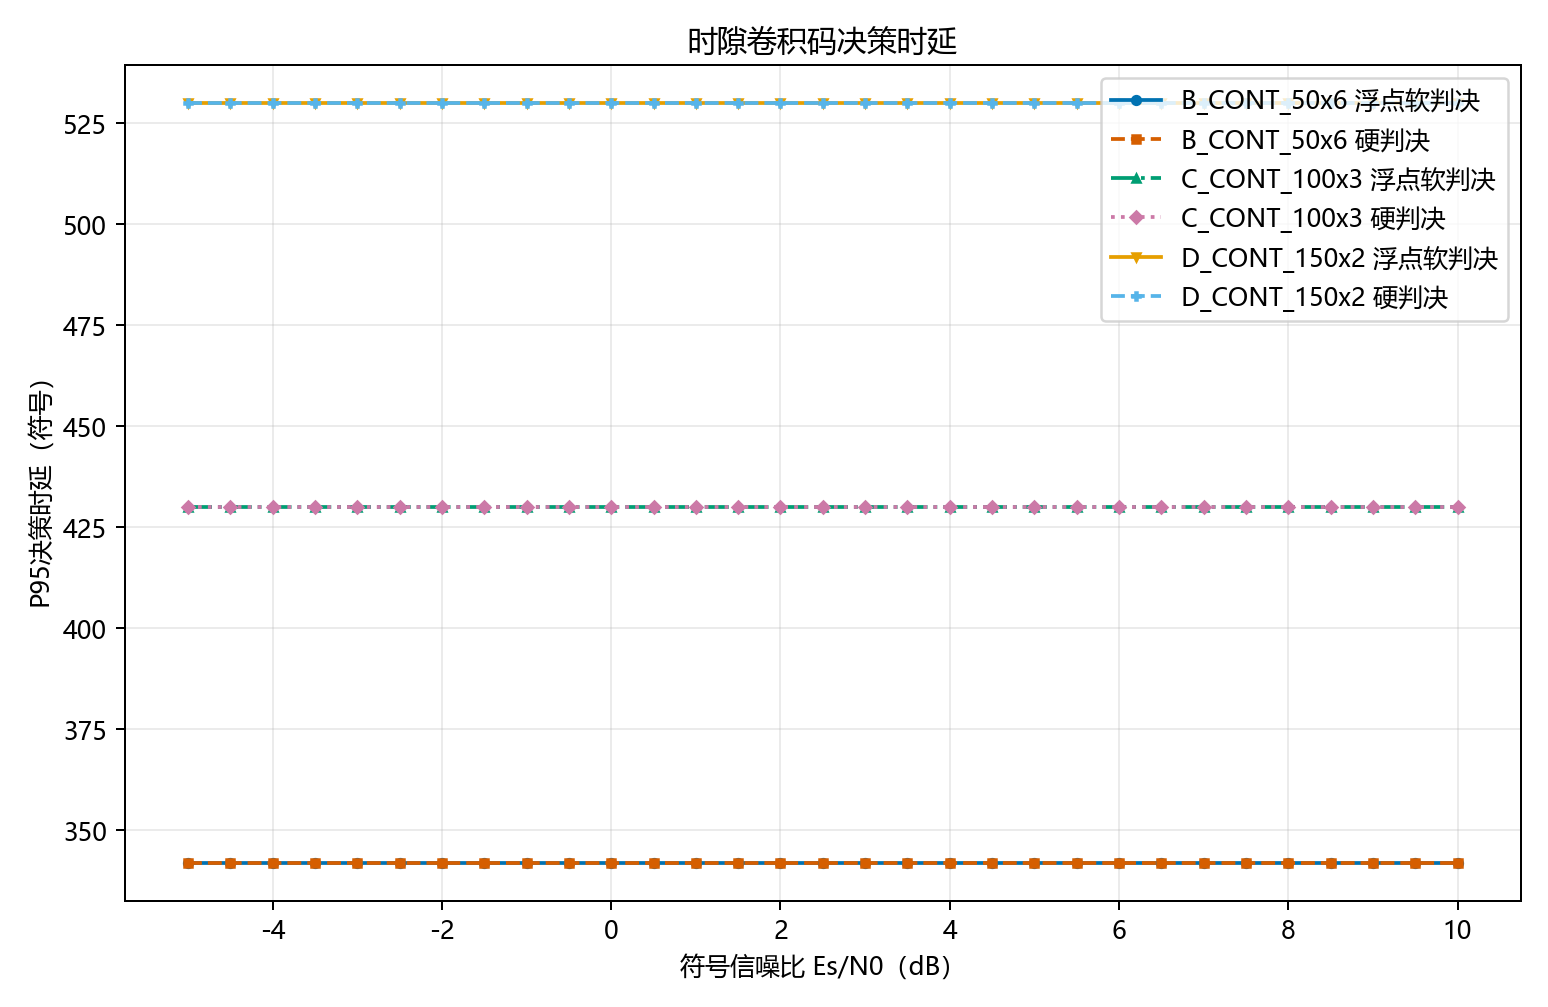
\includegraphics[width=0.98\linewidth]{../Task/Comparison/S6/results/summary/figures/cc_08_decision_delay/figure.png}\\[-0.2em]\small（c）决策时延
  \end{minipage}
  \caption{卷积码Viterbi译码的软件时间与流式输出时延}
  \label{fig:s6-cc-latency}
\end{figure}

\begin{table}[htbp]
  \centering
  \scriptsize
  \caption{硬判决与浮点软判决Viterbi的计算结构和实现代价}
  \label{tab:s6-cc-cost}
  \setlength{\tabcolsep}{2.0pt}
  \begin{tabular}{p{0.11\textwidth}p{0.18\textwidth}p{0.17\textwidth}p{0.14\textwidth}p{0.13\textwidth}p{0.17\textwidth}}
    \toprule
    判决 & 分支度量 & 共同骨架 & 整块加权平均/$\mu$s & 整块最大/$\mu$s & 工程特征 \\
    \midrule
    硬判决 & 0/1比特与汉明距离 & 相同状态、候选分支、ACS和回溯 & 339.03 & 34231.5 & 计算精度要求低，可靠性损失较大 \\
    浮点软判决 & 连续符号与欧氏距离平方 & 相同状态、候选分支、ACS和回溯 & 524.00 & 65607.2 & 保留幅值可靠性信息，分支度量更重 \\
    \bottomrule
  \end{tabular}
\end{table}

\subsection{卷积码工程结论}

浮点软判决以更重的分支度量换取约2.10--2.26 dB的FER门限收益，适合链路可靠性优先、具备浮点或等效定点度量资源的接收机。硬判决降低输入精度和分支度量实现要求，适合资源或实时性更受约束且链路余量足够的场景。连续窗口方案减小模型内存并提供分批输出，但窗口重复计算使当前串行软件时间高于整块方案；首输出与决策时延应作为独立流式指标使用。

\section{LDPC BP与NMS译码对比}

\subsection{正式配置与配对条件}

S6采用BG2 Direct QC-LDPC的N560实例。老师给出的名义目标长度为576 bit，Direct BG2候选选择器最终映射到实际长度560 bit，因此本章与图表均称为N560。载荷为300 bit，实际码率为$300/560=0.5357$，提升因子$Z_c=56$，信息容量448 bit，填充148 bit，校验长度112 bit，校验子矩阵秩为112。BP与NMS的最大迭代次数均为32，均在完成一次完整迭代后计算综合征并提前停止，NMS归一化系数为$\alpha=0.95$。

\begin{table}[htbp]
  \centering
  \scriptsize
  \caption{S6 LDPC译码算法比较配置}
  \label{tab:s6-ldpc-config}
  \setlength{\tabcolsep}{2.4pt}
  \begin{tabular}{p{0.17\textwidth}p{0.20\textwidth}p{0.17\textwidth}p{0.20\textwidth}p{0.16\textwidth}}
    \toprule
    项目 & 数值 & 项目 & 数值 & 说明 \\
    \midrule
    实际案例 & N560 & 载荷/码长 & 300/560 bit & 名义目标576映射到实际560 \\
    实际码率 & 0.5357 & $Z_c$ & 56 & BG2 Direct QC-LDPC \\
    填充/校验 & 148/112 bit & $\mathrm{rank}(H_p)$ & 112 & 不使用速率匹配与交织 \\
    译码器 & 分层BP、分层NMS & 最大迭代 & 32 & 完整迭代后综合征提前停止 \\
    NMS系数 & $\alpha=0.95$ & 配对输入 & 载荷、码字、LLR & 31个信噪比点哈希一致 \\
    \bottomrule
  \end{tabular}
\end{table}

BP和NMS共享同一载荷、码字、噪声、对数似然比（Log-Likelihood Ratio，LLR）、校验图、最大迭代次数和提前停止规则，只改变校验节点消息更新。逐信噪比的载荷、码字和LLR哈希均一致，使该对比能够把可靠性与时间差异较严格地归因于校验节点更新结构。

\subsection{BER与FER}

图\ref{fig:s6-ldpc-reliability}中BP与NMS曲线在瀑布区基本重合，NMS表现出轻微性能损失。FER为0.1时，BP和NMS所需$E_s/N_0$分别为4.541 dB和4.577 dB，NMS损失0.036 dB；FER为0.01时，两者分别为5.866 dB和5.875 dB，损失0.010 dB。两种算法各有4个零BER/FER工作点，零值没有用于门限外推。当前$\alpha=0.95$配置因此在两个目标FER处保留了接近BP的可靠性。

\begin{figure}[p]
  \centering
  \begin{minipage}{0.92\textwidth}\centering
    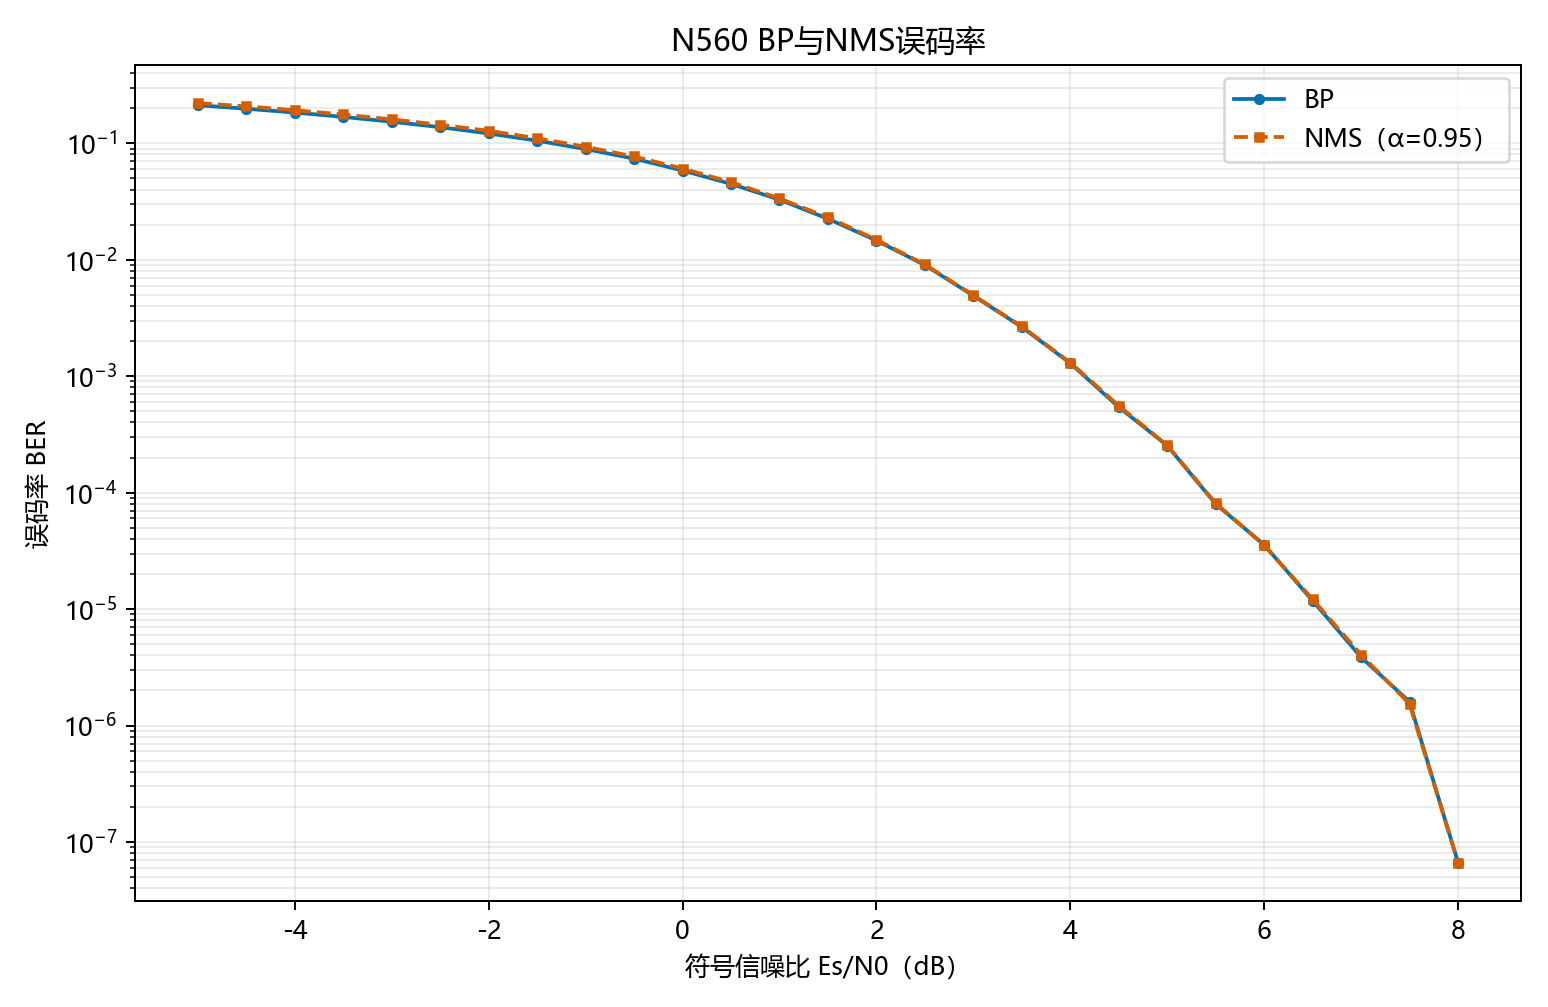
\includegraphics[width=0.90\linewidth]{../Task/Comparison/S6/results/summary/figures/ldpc_01_ber/figure.png}\\[-0.2em]\small（a）比特错误率
  \end{minipage}\par\medskip
  \begin{minipage}{0.92\textwidth}\centering
    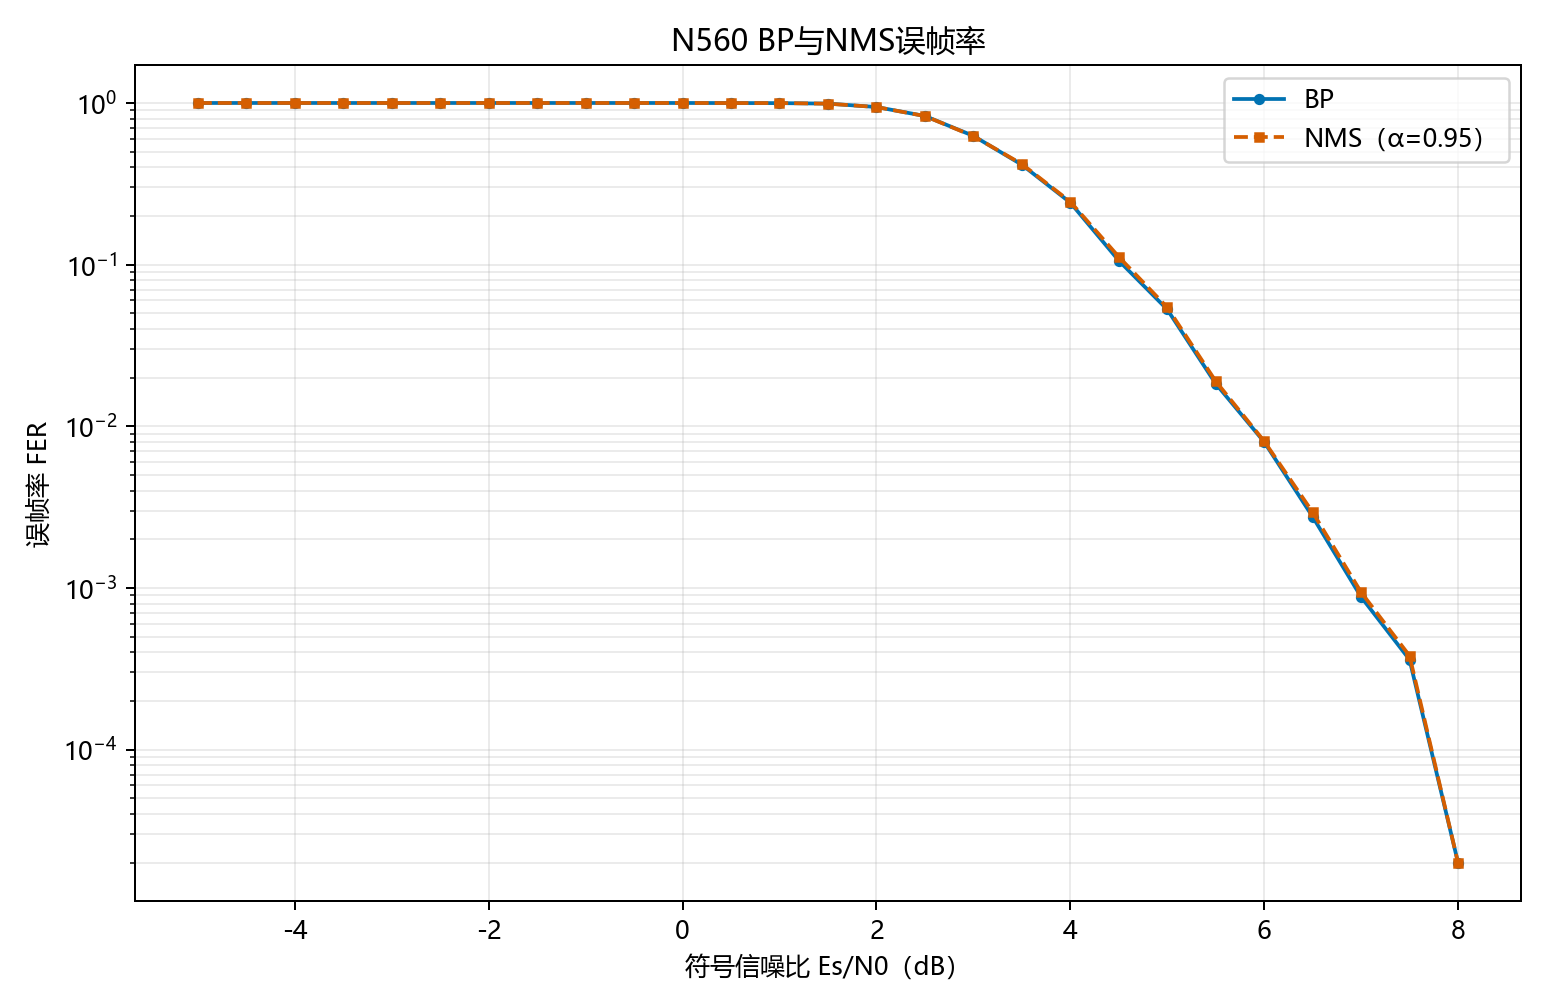
\includegraphics[width=0.90\linewidth]{../Task/Comparison/S6/results/summary/figures/ldpc_02_fer/figure.png}\\[-0.2em]\small（b）帧错误率
  \end{minipage}
  \caption{LDPC BP与NMS译码的BER和FER}
  \label{fig:s6-ldpc-reliability}
\end{figure}

\subsection{迭代与提前停止行为}

图\ref{fig:s6-ldpc-convergence}表明，低信噪比区的大量帧达到32次上限，进入瀑布区后平均迭代数随可靠性提高而下降，提前停止率相应上升。31点等权网格均值中，BP和NMS平均迭代数分别为16.44和13.11；其逐点范围分别为1--32次和1--28.47次。NMS在部分低信噪比点出现较高提前停止率，其中可能包含错误码字满足校验的情况，不能把“提前停止”单独解释为可靠译码成功。总软件代价同时取决于迭代次数和单次迭代计算结构，不能只用平均迭代数判断复杂度。

\begin{figure}[p]
  \centering
  \begin{minipage}{0.92\textwidth}\centering
    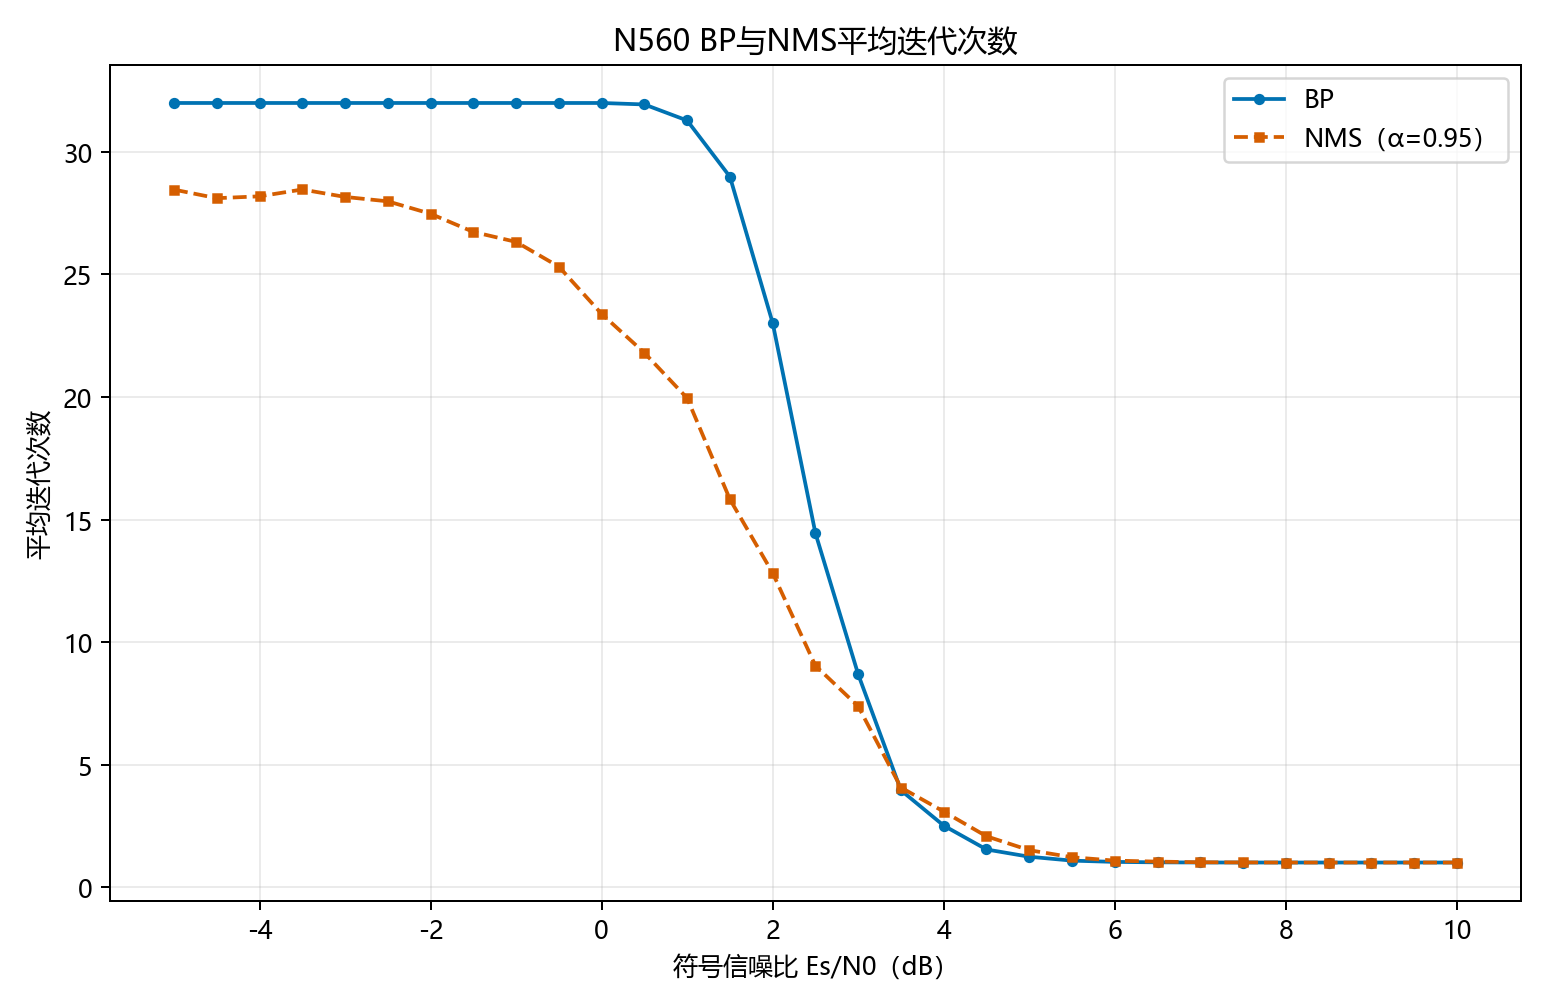
\includegraphics[width=0.90\linewidth]{../Task/Comparison/S6/results/summary/figures/ldpc_03_iterations/figure.png}\\[-0.2em]\small（a）平均迭代次数
  \end{minipage}\par\medskip
  \begin{minipage}{0.92\textwidth}\centering
    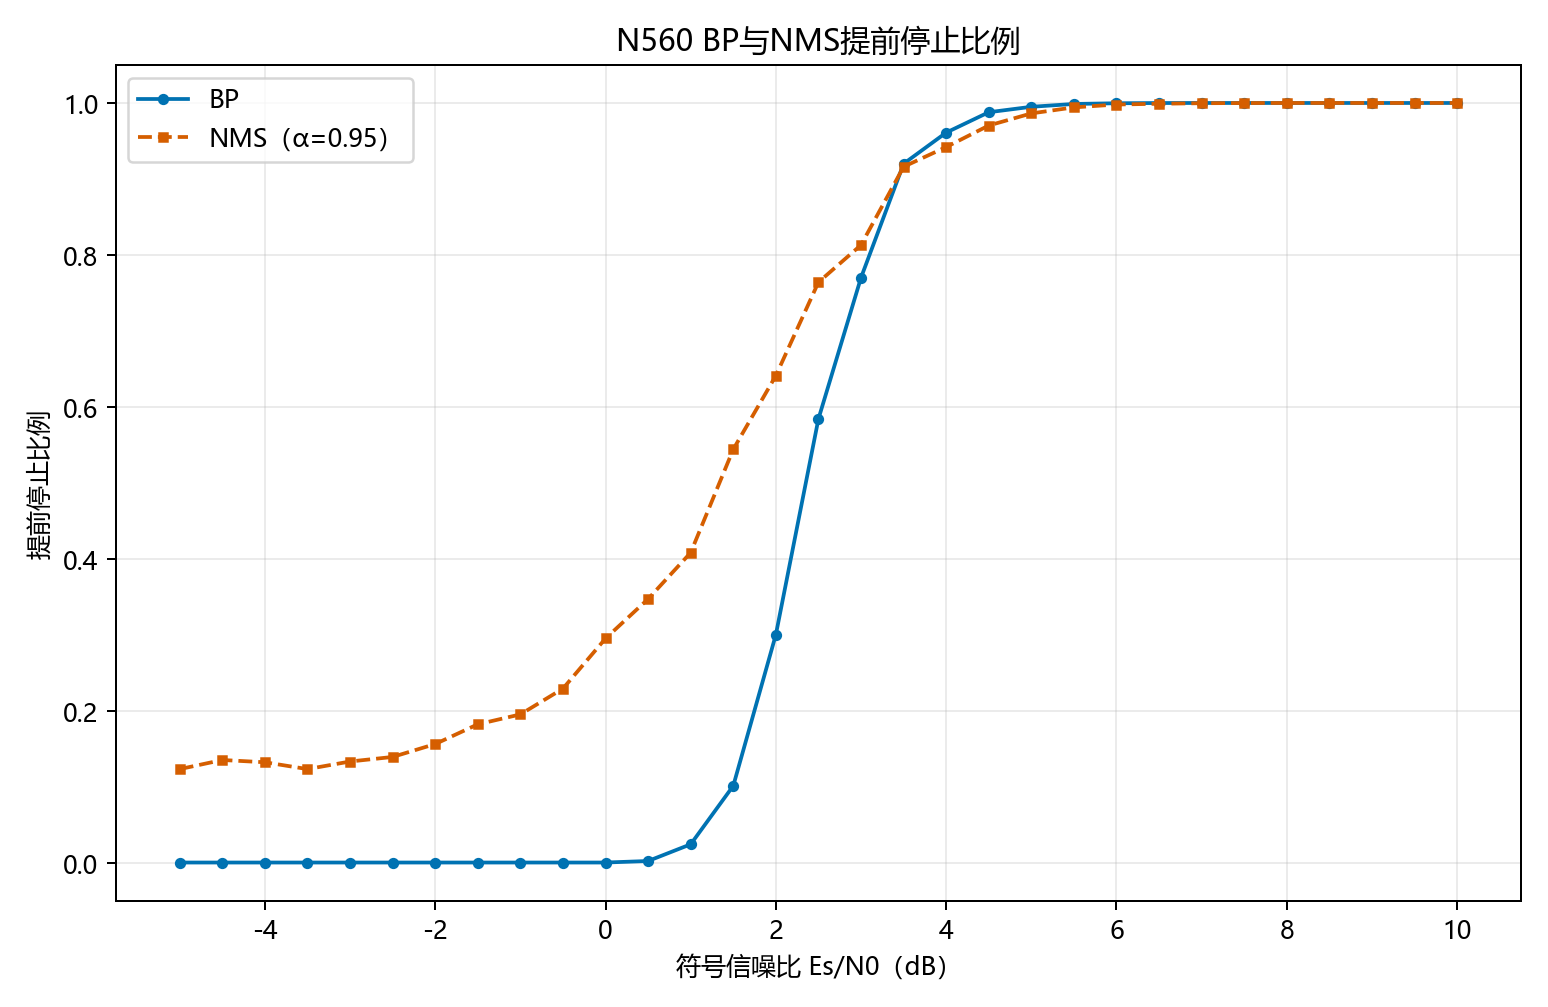
\includegraphics[width=0.90\linewidth]{../Task/Comparison/S6/results/summary/figures/ldpc_04_early_stop/figure.png}\\[-0.2em]\small（b）提前停止率
  \end{minipage}
  \caption{LDPC BP与NMS的迭代和提前停止行为}
  \label{fig:s6-ldpc-convergence}
\end{figure}

\subsection{复杂度、存储与软件译码时间}

BP校验节点更新包含双曲正切、反双曲正切及消息更新；NMS以绝对值、符号、第一/第二最小值、比较和$\alpha$缩放近似非线性更新。图\ref{fig:s6-ldpc-cost}中的网格平均操作计数显示，BP每帧约25780.66次双曲正切和12890.33次反双曲正切；NMS每帧约10280.70次绝对值、20561.41次比较和6190.30次最小值操作，并包含符号与缩放。二者同为一次事件并不意味着处理器代价相同，尤其不能把双曲函数和比较操作作为统一单位相加。

两种译码器的消息与后验缓冲布局相同，模型内存均为11312 byte。按全部工作点帧数加权，BP与NMS平均译码时间分别为140.687~$\mu$s和33.157~$\mu$s，NMS减少76.4\%，约为BP的23.6\%；最大观测时间分别为34024.9~$\mu$s和9468.0~$\mu$s，NMS减少72.2\%。逐点平均时间曲线还表明，低信噪比满迭代区域的BP时间可超过2 ms，而NMS保持在0.5 ms以内。该差异同时来自更轻的单次校验节点更新和实际迭代行为。

\begin{figure}[p]
  \centering
  \begin{minipage}{0.49\textwidth}\centering
    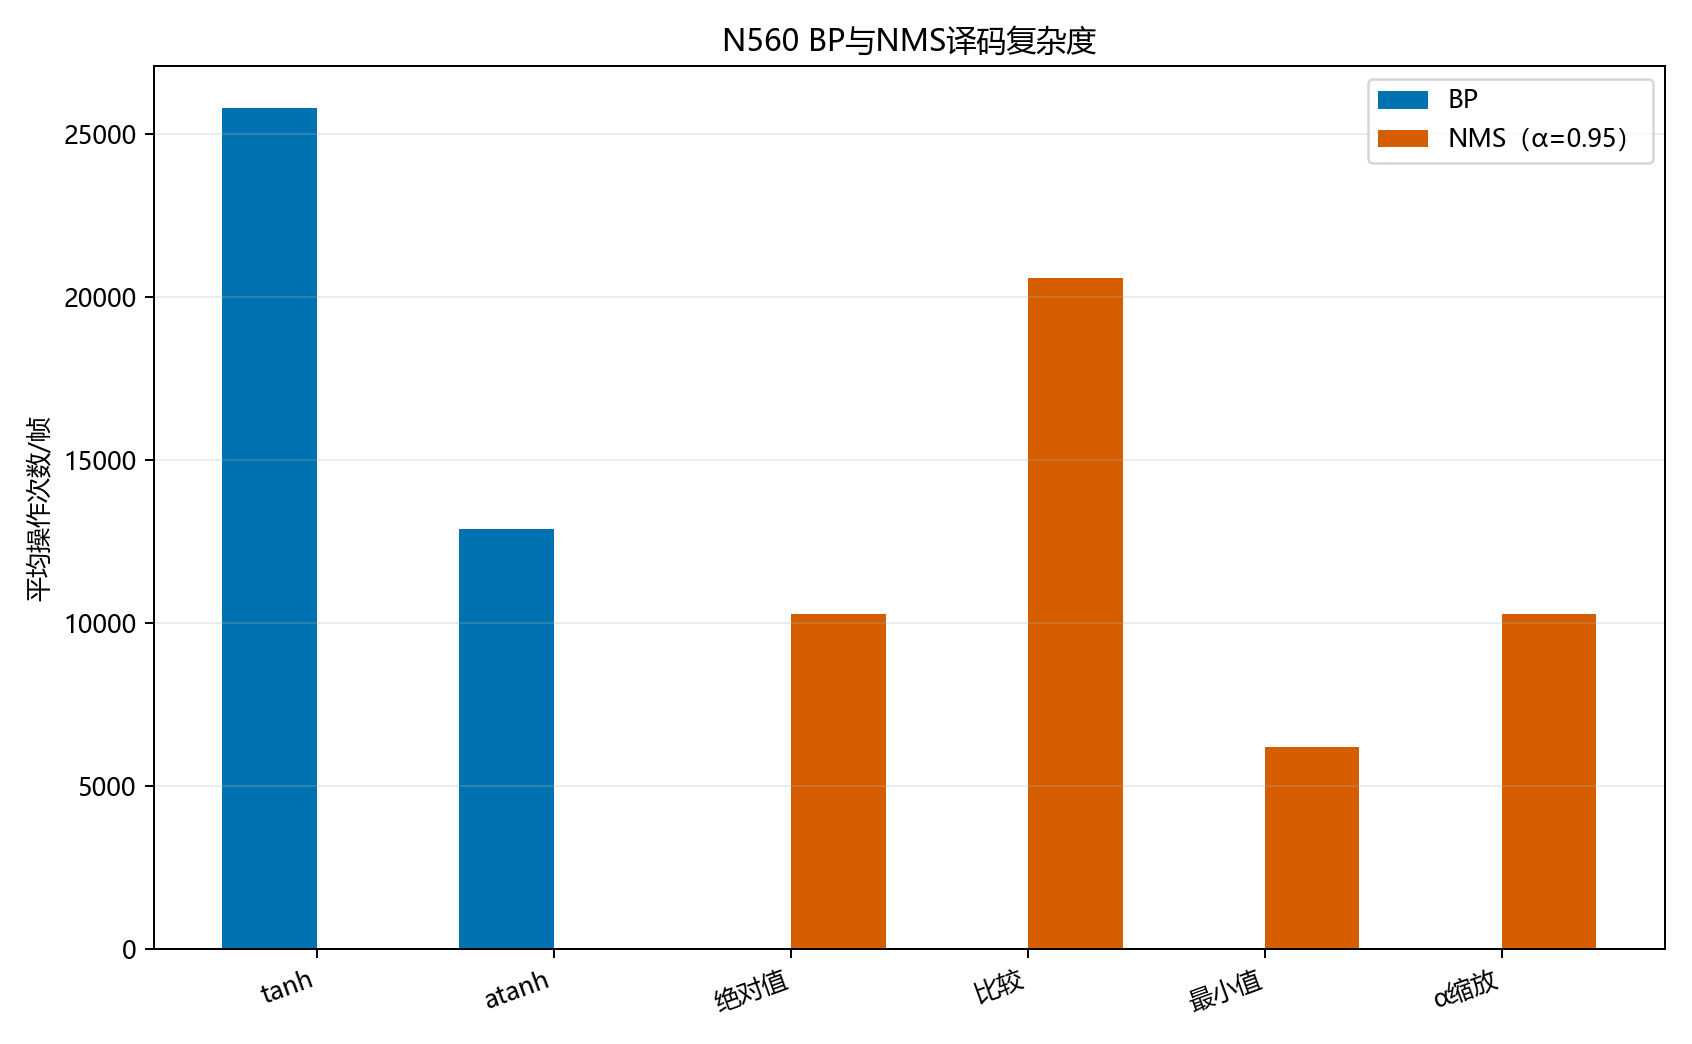
\includegraphics[width=0.98\linewidth]{../Task/Comparison/S6/results/summary/figures/ldpc_05_complexity/figure.png}\\[-0.2em]\small（a）主要操作结构
  \end{minipage}\hfill
  \begin{minipage}{0.49\textwidth}\centering
    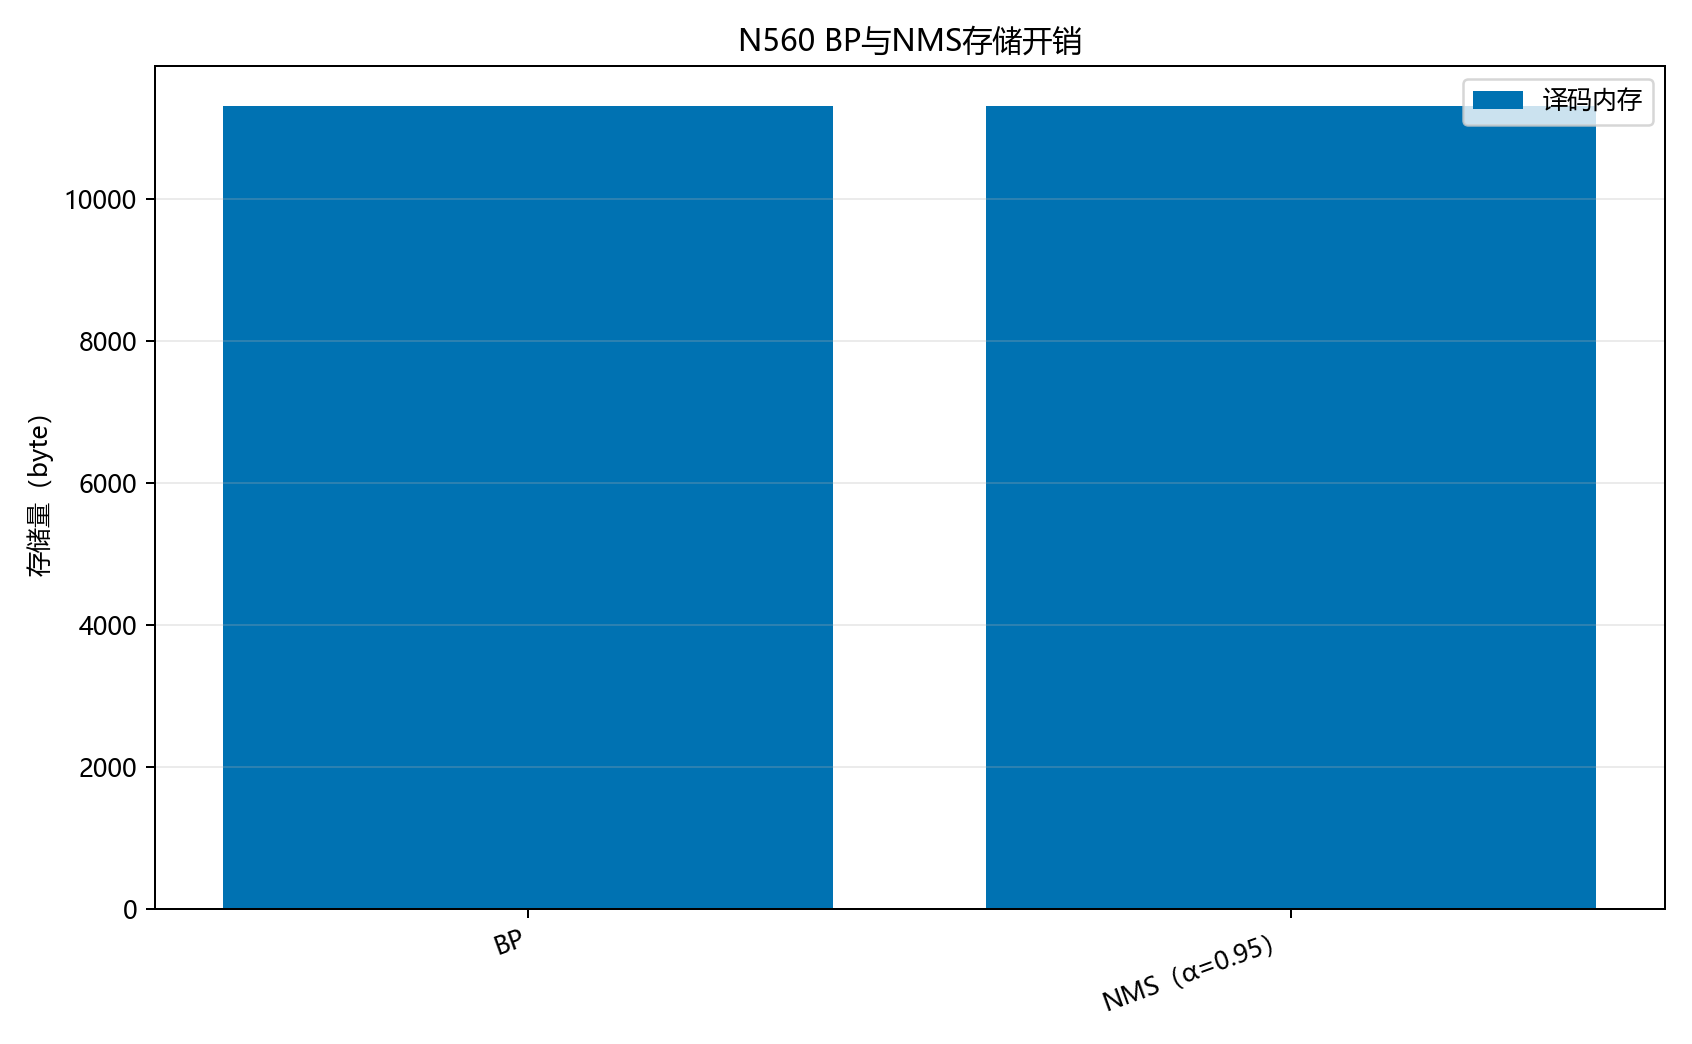
\includegraphics[width=0.98\linewidth]{../Task/Comparison/S6/results/summary/figures/ldpc_06_memory/figure.png}\\[-0.2em]\small（b）译码器内存
  \end{minipage}\par\medskip
  \begin{minipage}{0.49\textwidth}\centering
    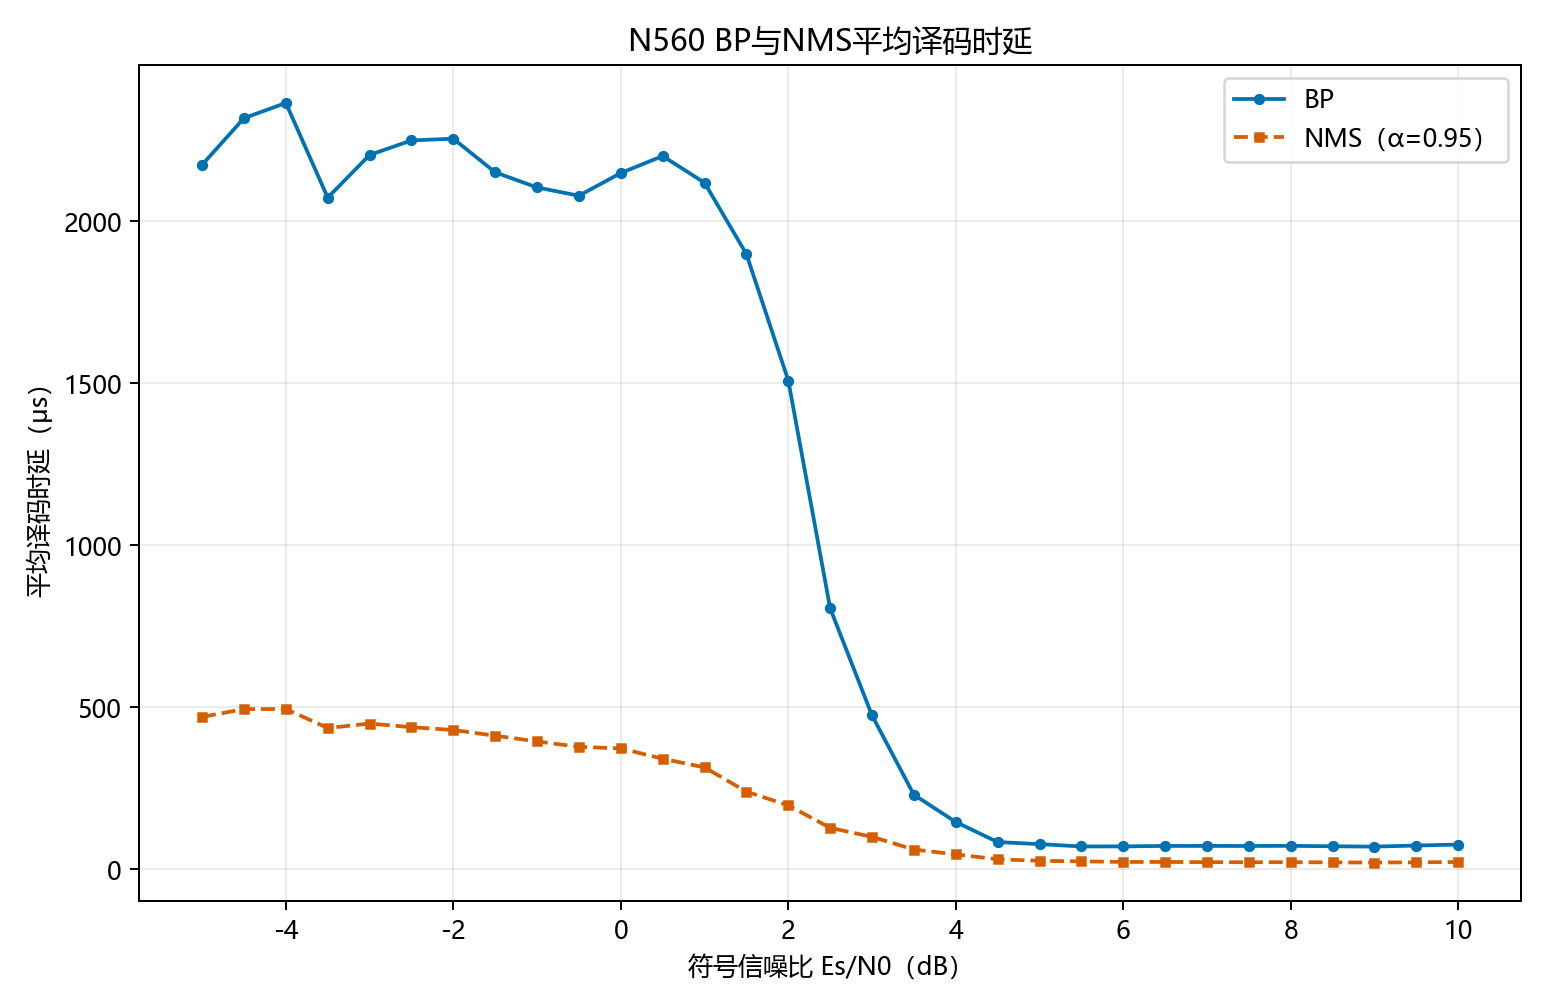
\includegraphics[width=0.98\linewidth]{../Task/Comparison/S6/results/summary/figures/ldpc_07_avg_time/figure.png}\\[-0.2em]\small（c）平均译码时间
  \end{minipage}\hfill
  \begin{minipage}{0.49\textwidth}\centering
    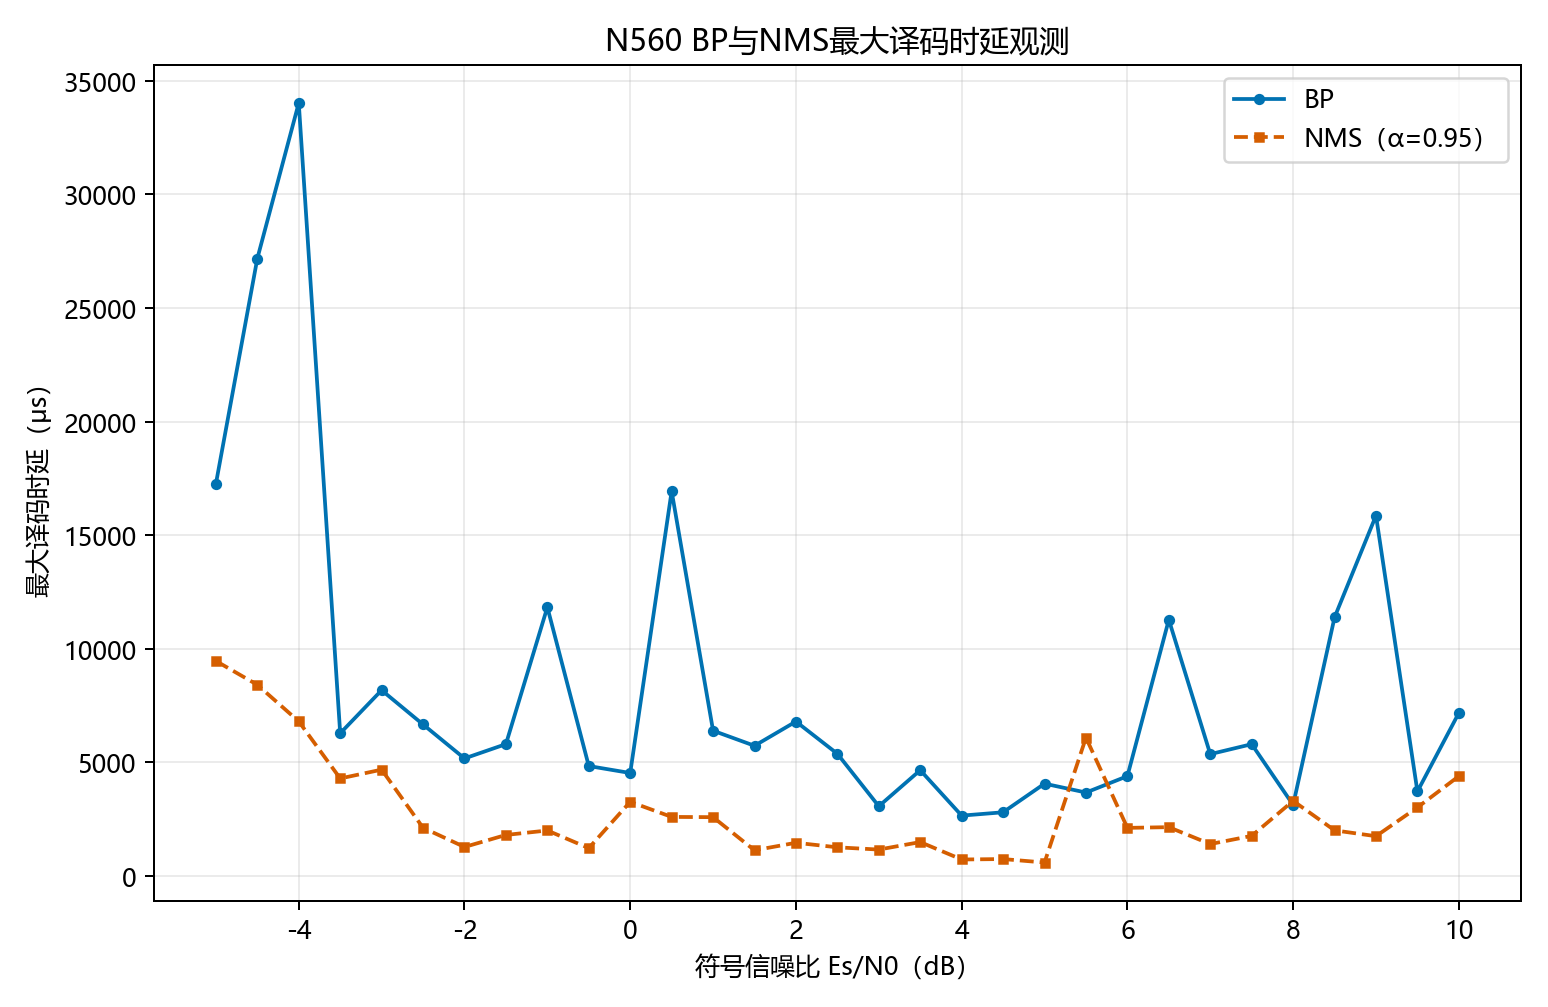
\includegraphics[width=0.98\linewidth]{../Task/Comparison/S6/results/summary/figures/ldpc_08_max_time/figure.png}\\[-0.2em]\small（d）最大观测译码时间
  \end{minipage}
  \caption{LDPC BP与NMS的计算结构、存储和软件时间}
  \label{fig:s6-ldpc-cost}
\end{figure}

\begin{table}[htbp]
  \centering
  \scriptsize
  \caption{LDPC BP与NMS的可靠性、复杂度和时间指标}
  \label{tab:s6-ldpc-summary}
  \setlength{\tabcolsep}{2.0pt}
  \begin{tabular}{p{0.08\textwidth}cccccc p{0.18\textwidth}}
    \toprule
    译码器 & FER=0.1/dB & FER=0.01/dB & 网格平均迭代 & 加权平均/$\mu$s & 最大/$\mu$s & 内存/byte & 校验节点主要运算 \\
    \midrule
    BP & 4.541 & 5.866 & 16.44 & 140.687 & 34024.9 & 11312 & 双曲正切、反双曲正切、消息更新 \\
    NMS & 4.577 & 5.875 & 13.11 & 33.157 & 9468.0 & 11312 & 绝对值、比较、最小值、符号和缩放 \\
    \bottomrule
  \end{tabular}
\end{table}

\subsection{LDPC工程结论}

BP提供当前实现的可靠性基准，其非线性校验节点更新带来较高软件计算代价。NMS以最小值近似和归一化系数简化校验节点更新，在FER为0.1和0.01时仅损失0.036 dB和0.010 dB，同时将加权平均和最大观测软件译码时间分别降低76.4\%和72.2\%，且不增加模型内存。对于本项目N560、$\alpha=0.95$和32次迭代上限的配置，NMS形成了可靠性损失很小而软件时间明显下降的工程替代；该判断不外推到其他码长、系数或硬件实现。

\section{三类译码实现的工程特征综合}

表\ref{tab:s6-engineering-summary}按编码族总结可靠性、计算、存储与时间特征，不建立跨族BER或操作计数排名。三类任务的载荷、码长、图结构和操作语义不同，BCH的一次有限域乘法、Viterbi的一次ACS与LDPC的一次比较不具有统一成本。软件时间和模型内存虽然使用共同单位，也只反映当前软件环境和各自计时、建模范围，不能直接替代目标硬件评估。

\begin{table}[htbp]
  \centering
  \scriptsize
  \caption{三类译码实现的工程特征汇总}
  \label{tab:s6-engineering-summary}
  \setlength{\tabcolsep}{1.7pt}
  \begin{tabular}{p{0.07\textwidth}p{0.12\textwidth}p{0.13\textwidth}p{0.15\textwidth}p{0.11\textwidth}p{0.12\textwidth}p{0.11\textwidth}}
    \toprule
    编码族 & 译码器 & 可靠性特征 & 主要计算结构 & 存储特征 & 软件时间特征 & 适用倾向 \\
    \midrule
    BCH & 分组查表 & 当前完整方案门限较高 & 短综合征、查表、翻转 & 固定表与小工作区 & 平均时间较低 & 结构固定、资源受限 \\
    BCH & BM与Chien & 当前完整方案门限降低 & 综合征、BM、Chien、有限域运算 & 有限域表与代数状态增加 & 平均时间增加 & 整块纠错能力优先 \\
    卷积码 & 硬判决Viterbi & 损失幅值可靠性信息 & 汉明度量、ACS、回溯 & 与同组织软判决相同 & 分支度量较轻 & 资源或实时性优先 \\
    卷积码 & 浮点软判决Viterbi & FER门限改善约2.1--2.3 dB & 欧氏度量、ACS、回溯 & 与同组织硬判决相同 & CPU时间增加 & 可靠性优先 \\
    LDPC & 分层BP & 可靠性基准 & 非线性校验节点和消息更新 & 消息缓冲11312 byte & 当前实现较慢 & 性能基准与高精度实现 \\
    LDPC & 分层NMS & 门限损失不超过0.04 dB & 最小值、符号和归一化 & 消息缓冲11312 byte & 平均时间降低76.4\% & 低复杂度软件实现 \\
    \bottomrule
  \end{tabular}
\end{table}

从同族选择看，BCH需要在短分组查表的低实现代价与整块代数方案的纠错收益之间权衡；卷积码需要在软信息带来的约2 dB可靠性收益与分支度量开销之间权衡；LDPC则体现出NMS以很小门限损失换取显著软件加速的特点。工程选型应把BER、FER、操作结构、存储、平均时间和最大观测时间同时纳入，而不是只根据一条误码曲线作结论。

\section{本章结论}

BCH比较表明，分组综合征查表适合短分组和固定结构，BCH-S200以较小内存和较低软件时间完成译码；BM与Chien搜索适合较长整块BCH，BCH-B200在FER为0.01时节省1.671 dB，但平均译码时间和模型内存分别增加70.5\%和52.4\%。该BER/FER差异属于两套完整方案的综合差异，不能纯归因于译码器。

卷积码比较表明，浮点软判决保留连续接收幅值的可靠性信息，在FER为0.1和0.01时相对硬判决分别获得2.098 dB和2.260 dB收益；代价是整块加权平均CPU译码时间增加54.6\%，分支度量需要浮点减法、平方和加法。硬判决适合计算精度与实时资源更紧、同时链路余量允许可靠性损失的场景。连续方案的首输出和决策时延属于符号调度指标，不能与CPU墙钟时间混称。

LDPC比较表明，BP是当前N560配置的性能基准，NMS通过最小值、符号和$\alpha=0.95$缩放替代非线性校验节点计算。NMS在两个目标FER处的损失均小于0.04 dB，加权平均和最大观测软件译码时间分别降低76.4\%和72.2\%，模型内存保持不变。复杂度判断必须同时考虑单次迭代结构与实际迭代次数。

三类结果共同说明，译码器选择需要同时满足可靠性、计算复杂度、存储和实时性约束。误码曲线回答链路余量问题，操作计数揭示实现结构，平均时间描述常态软件负担，最大观测时间暴露尾部风险；只有在保持各指标定义与比较边界的前提下，才能形成可追溯的工程选择。

\chapter{交织抗突发错误影响仿真}\label{chap:interleaving}
\captionsetup{font=small,labelfont=normalfont,skip=0.6em}

\section{交织抗突发错误实验设计}

本章在固定编码器、译码器和调制方式的条件下，研究交织映射对连续突发错误的影响。研究对象包括200 bit低速分块BCH方案和300 bit卷积码方案；前者采用19个BCH(15,11,1)子块，后者采用终止整帧浮点软判决Viterbi译码。实验变量限定为交织方法、交织参数、突发长度和突发位置，编码码本与译码算法均保持不变。因此，本章评价的是交织对错误空间分布以及观测BER、FER的影响，而不是编码器理论纠错能力的变化。

图\ref{fig:s7-chain-visio}给出统一仿真链路。编码比特先经过交织和BPSK映射，再进入突发错误信道；接收端完成硬判决或软信息形成后，先按逆置换恢复译码顺序，再调用相应译码器。突发错误直接作用于交织后的发送符号序列，因而同一连续信道异常在不同逆置换下会形成不同的译码器输入位置分布。

\begin{figure}[htbp]
  \centering
  \fbox{\begin{minipage}[c][0.11\textheight][c]{0.90\textwidth}
    \centering\bfseries 交织抗突发错误统一处理链路\\[0.7em]
    输入信息比特 $\rightarrow$ 信道编码 $\rightarrow$ 交织 $\rightarrow$ BPSK
    $\rightarrow$ 突发错误信道 $\rightarrow$ 硬/软判决\\[0.35em]
    $\rightarrow$ 去交织 $\rightarrow$ 信道译码
    $\rightarrow$ BER / FER / 突发错误容限 / 缓冲与时间\\[0.45em]
    \normalfont\small 突发错误信道：连续极性反转 + AWGN
  \end{minipage}}
  \caption{交织抗突发错误仿真链路}
  \label{fig:s7-chain-visio}
\end{figure}

正式仿真采用成对比较。相同$E_s/N_0$、突发比例和突发位置构成一个公平性组，组内各交织配置共享输入信息、标准母噪声、突发起点和帧序列。BCH与卷积码合计1116个比较组均通过一致性核验，因此组内性能差异可以主要归因于交织映射变化。停止条件同时受最少帧数、目标错误帧数和最大帧数约束，避免不同配置使用不一致的样本边界。

\section{固定编码配置、突发错误信道与交织方法}

\subsection{固定编码方案}

表\ref{tab:s7-unified-conditions}列出正式展示范围。$E_s/N_0$从$-5$ dB到$10$ dB，步长为$0.5$ dB。报告只使用2\%和5\%两档突发条件：对285 bit BCH码字，对应连续6 bit和14 bit；对612 bit卷积码码字，对应连续12 bit和31 bit。位置变量覆盖帧首、四分之一、帧中、四分之三、帧尾和固定随机位置。

\begin{table}[htbp]
  \centering
  \caption{S7统一仿真条件}
  \label{tab:s7-unified-conditions}
  \small
  \begin{tabular}{p{0.22\textwidth}p{0.33\textwidth}p{0.35\textwidth}}
    \toprule
    参数 & 取值 & 说明 \\
    \midrule
    调制方式 & BPSK & 编码比特0映射为$+1$，1映射为$-1$ \\
    信道 & 突发错误信道叠加AWGN & 连续区间极性反转，全帧叠加高斯噪声 \\
    $E_s/N_0$ & $-5\sim10$ dB，步长$0.5$ dB & 共31个正式点 \\
    突发比例 & 2\%、5\% & BCH为6、14 bit；卷积码为12、31 bit \\
    突发位置 & 帧首、$1/4$、帧中、$3/4$、帧尾、随机 & 作用于交织后的发送序列 \\
    停止规则 & 1000帧；200错误帧；最多50000帧 & 成对停止与共享帧序列 \\
    公平性审计 & 1116组，0项失败 & 组内共享输入、噪声、起点和帧序列 \\
    \bottomrule
  \end{tabular}
\end{table}

固定编码方案见表\ref{tab:s7-fixed-codes}。BCH链路在200 bit有效载荷后填充9 bit，形成19个11 bit信息子块，分别编码为19个15 bit码字，总发送长度285 bit，实际码率为$200/285\approx0.701754$。卷积码链路对300 bit有效载荷添加6个零尾比特，形成306个trellis step和612个编码比特，实际码率为$300/612\approx0.490196$。高速参考采用LDPC BG2、$Z=40$、发送长度640 bit，其作用范围限定为无交织、无突发AWGN近码率比较。

\begin{table}[htbp]
  \centering
  \caption{S7固定编码方案}
  \label{tab:s7-fixed-codes}
  \footnotesize
  \resizebox{\textwidth}{!}{%
  \begin{tabular}{lrrrrp{5.0cm}}
    \toprule
    方案 & 有效载荷/bit & 填充或尾比特 & 发送长度/bit & 实际码率 & 结构与译码器 \\
    \midrule
    分块BCH & 200 & 9 & 285 & 0.701754 & $19\times$BCH(15,11,1)，综合校验查表硬判决 \\
    卷积码 & 300 & 6 & 612 & 0.490196 & $K=7$，$G=(171,133)_8$，终止整帧浮点软Viterbi \\
    LDPC高速基线 & 300 & 20 & 640 & 0.468750 & BG2，$Z=40$，layered NMS，$\alpha=0.80$，最多32次迭代 \\
    \bottomrule
  \end{tabular}}
\end{table}

\subsection{突发错误信道模型与正式仿真条件}

对编码比特$c_i$，BPSK映射定义为
\begin{equation}
  x_i=\begin{cases}
  +1, & c_i=0,\\
  -1, & c_i=1.
  \end{cases}
\end{equation}
突发错误信道的接收符号为
\begin{equation}
  y_i=h_i x_i+n_i,
  \qquad
  h_i=\begin{cases}
  -1, & s\le i<s+B,\\
  +1, & \text{其他位置},
  \end{cases}
\end{equation}
其中$s$为突发起点，$B$为连续突发长度。全帧噪声满足
\begin{equation}
  n_i\sim\mathcal{N}(0,\sigma^2),
  \qquad
  \sigma^2=\frac{1}{2\times10^{(E_s/N_0)_{\mathrm{dB}}/10}}.
\end{equation}
该模型在长度为$B$的连续区间内反转BPSK符号极性，区间外保持原极性，同时对全帧叠加AWGN，由此形成连续、位置可控且长度可控的突发错误条件。信道输入已经完成交织，去交织操作位于判决或软信息形成之后，因此交织的直接作用是把连续异常重新映射到译码器输入空间。

\subsection{BCH交织方法}

表\ref{tab:s7-bch-interleavers}给出BCH正式配置。三种交织方案均覆盖完整285 bit码字并需要暂存285个编码比特，但排列结构不同。子块结构交织利用19个BCH子块的组织关系；行列交织将全帧按15行写入后按列读出；全帧伪随机交织采用固定种子的确定性置换。这里的缓存量只表示结构上的编码比特暂存深度，不表示物理传输时延。

\begin{table}[htbp]
  \centering
  \caption{BCH正式交织方案定义}
  \label{tab:s7-bch-interleavers}
  \small
  \resizebox{\textwidth}{!}{%
  \begin{tabular}{p{0.24\textwidth}p{0.14\textwidth}rrp{0.35\textwidth}}
    \toprule
    配置 & 参数 & 跨度/bit & 缓存/bit & 映射特征 \\
    \midrule
    无交织 & 0 & 1 & 0 & 恒等映射 \\
    BCH子块结构交织 & $D=19$ & 285 & 285 & 按19个15 bit子块组织并列读 \\
    全帧行列交织 & $R=15$ & 285 & 285 & 全帧行写列读 \\
    全帧伪随机交织 & 285 & 285 & 285 & 固定种子的全帧确定性置换 \\
    \bottomrule
  \end{tabular}}
\end{table}

\subsection{卷积码交织方法与跨度定义}

卷积码交织在trellis step层面保持每个母码输出对，不拆分同一步产生的两个编码比特。短深度块交织参数$D$决定局部窗口规模；本章中的$D$仅表示交织深度，不是Viterbi回溯深度。表\ref{tab:s7-cc-interleavers}中，$D=8$覆盖64个trellis step并缓存128个编码比特；$D=16$与局部伪随机span=128均覆盖128个trellis step并缓存256个编码比特。因而$D=8$与Pseudo128属于不同资源规模的工程配置比较，只有$D=16$与Pseudo128能够支持等跨度、等缓存条件下的排列方式受控比较。

\begin{table}[htbp]
  \centering
  \caption{卷积码正式交织方案定义}
  \label{tab:s7-cc-interleavers}
  \footnotesize
  \resizebox{\textwidth}{!}{%
  \begin{tabular}{p{0.23\textwidth}p{0.19\textwidth}rrrp{0.24\textwidth}}
    \toprule
    配置 & 方法 & trellis跨度 & 编码bit跨度 & 缓存/bit & 比较角色 \\
    \midrule
    无交织 & 恒等映射 & 1 & 2 & 0 & 基线 \\
    短深度$D=8$ & 规则块交织 & 64 & 128 & 128 & 工程配置 \\
    短深度$D=16$ & 规则块交织 & 128 & 256 & 256 & 等跨度受控 \\
    Pseudo128 & 局部伪随机 & 128 & 256 & 256 & 工程配置及等跨度受控 \\
    \bottomrule
  \end{tabular}}
\end{table}

\section{分块BCH交织抗突发错误结果}

\subsection{不同交织方法总体BER与FER}

图\ref{fig:s7-bch-burst-fer}比较2\%和5\%条件下的FER曲线。无交织配置在高信噪比区仍保留明显突发错误平台；子块结构交织和全帧行列交织则随$E_s/N_0$提高进入较低FER区。全帧伪随机交织的结果具有较强位置依赖，并未在本组测试中稳定达到两种规则结构交织的水平。这说明全帧跨度相同并不足以保证相同结果，置换与19个BCH子块边界的对应关系仍然重要。

\begin{figure}[htbp]
  \centering
  \begin{minipage}[t]{0.49\textwidth}
    \centering
    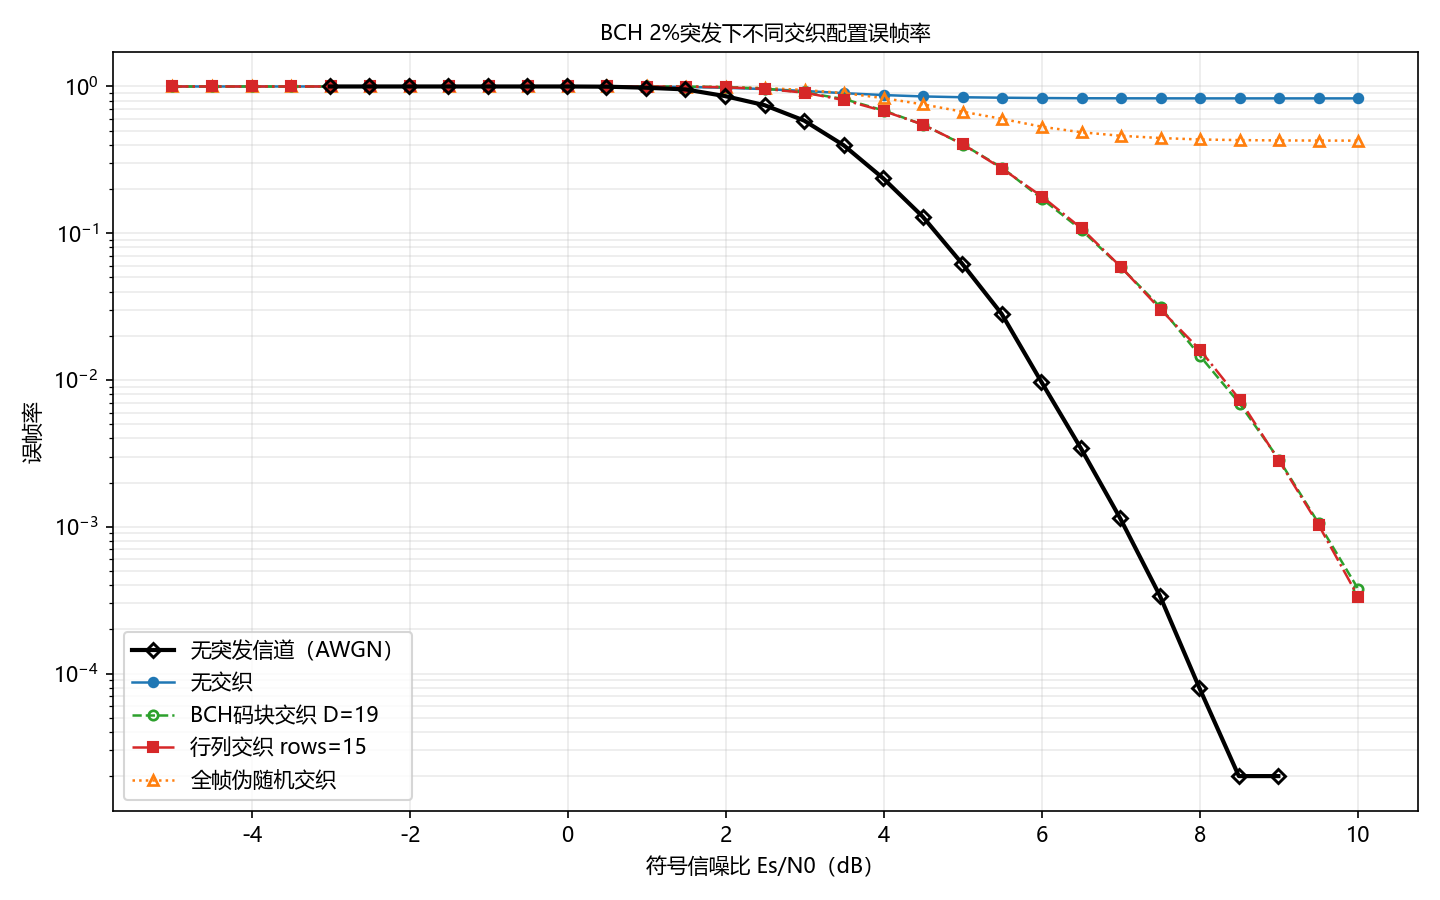
\includegraphics[width=\linewidth]{../Task/Comparison/S7/stage15_scientific_plots/results/bch/03_burst_2_fer/figure.png}\\[-0.2em]
    \small（a）2\%突发
  \end{minipage}
  \hfill
  \begin{minipage}[t]{0.49\textwidth}
    \centering
    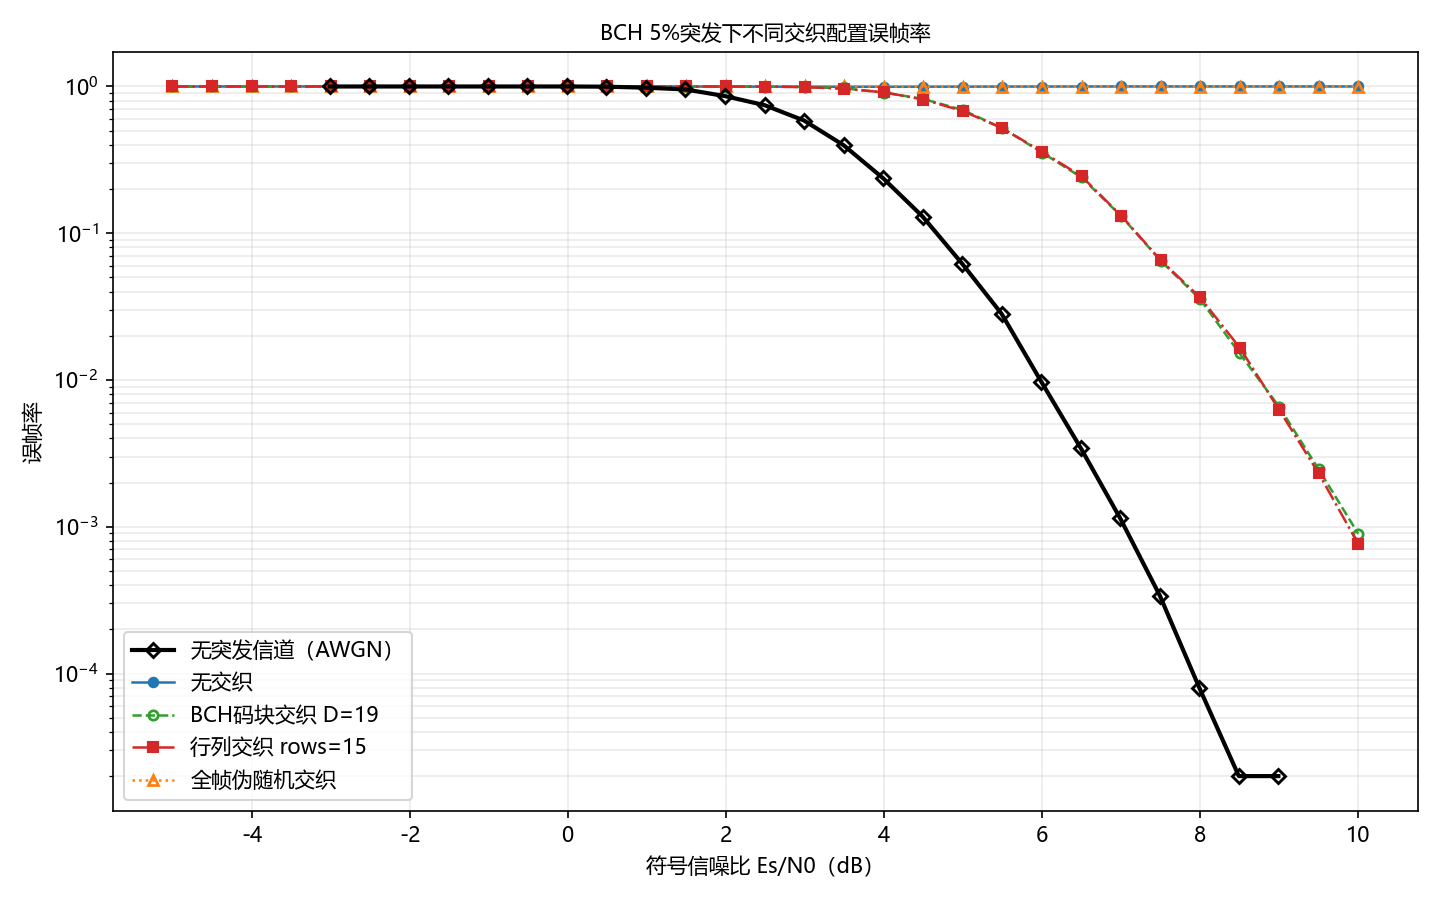
\includegraphics[width=\linewidth]{../Task/Comparison/S7/stage15_scientific_plots/results/bch/04_burst_5_fer/figure.png}\\[-0.2em]
    \small（b）5\%突发
  \end{minipage}
  \caption{分块BCH在两档突发长度下的误帧率}
  \label{fig:s7-bch-burst-fer}
\end{figure}

表\ref{tab:s7-bch-fer-improvement}给出$10$ dB代表点的六位置平均、最坏与最好FER。2\%条件下，无交织平均FER为0.829613，子块结构交织和行列交织分别降至$3.77\times10^{-4}$和$3.33\times10^{-4}$；5\%条件下，无交织FER为1，两种规则交织分别为$8.97\times10^{-4}$和$7.63\times10^{-4}$。对应平均FER相对降低率均超过99.9\%。全帧伪随机交织在2\%时平均FER为0.427587，在5\%时为0.998823，表现出置换结构和突发位置之间的强耦合。

\begin{table}[htbp]
  \centering
  \caption{BCH代表性FER改善（$E_s/N_0=10$ dB）}
  \label{tab:s7-bch-fer-improvement}
  \footnotesize
  \begin{tabular}{clrrrr}
    \toprule
    突发 & 配置 & 平均FER & 最坏FER & 最好FER & 相对降低/\% \\
    \midrule
    2\% & 无交织 & 0.829613 & 1 & $2.0\times10^{-5}$ & 0 \\
    2\% & 子块结构$D=19$ & $3.77\times10^{-4}$ & $4.40\times10^{-4}$ & $3.20\times10^{-4}$ & 99.9546 \\
    2\% & 行列$R=15$ & $3.33\times10^{-4}$ & $5.00\times10^{-4}$ & $1.80\times10^{-4}$ & 99.9598 \\
    2\% & 全帧伪随机 & 0.427587 & 0.99998 & $2.60\times10^{-4}$ & 48.4595 \\
    5\% & 无交织 & 1 & 1 & 1 & 0 \\
    5\% & 子块结构$D=19$ & $8.97\times10^{-4}$ & 0.00102 & $8.20\times10^{-4}$ & 99.9103 \\
    5\% & 行列$R=15$ & $7.63\times10^{-4}$ & $8.80\times10^{-4}$ & $6.20\times10^{-4}$ & 99.9237 \\
    5\% & 全帧伪随机 & 0.998823 & 1 & 0.99296 & 0.1177 \\
    \bottomrule
  \end{tabular}
\end{table}

\subsection{两档突发长度的影响}

从突发长度看，6 bit与14 bit连续异常对无交织BCH均构成强烈压力，但规则结构交织后的结果差异较小。$10$ dB时，子块结构交织由2\%条件的$3.77\times10^{-4}$上升到5\%条件的$8.97\times10^{-4}$，行列交织由$3.33\times10^{-4}$上升到$7.63\times10^{-4}$；两者的最坏位置FER仍不高于0.00102。由于BCH(15,11,1)只能保证纠正每个子块中的单比特错误，14 bit异常能否被有效处理取决于逆置换后每个子块获得的错误数，而不是只取决于总错误数。

全帧伪随机配置呈现不同特征。2\%条件下其最好位置FER已降到$2.60\times10^{-4}$，但最坏位置仍为0.99998，导致六位置平均FER为0.427587；5\%条件下最好位置也达到0.99296。该结果表明，固定伪随机置换可能在部分起点形成有利分散，却没有在所有代表位置上保持一致。规则结构交织把连续输入位置映射到可预期的子块关系，对本章19子块结构形成更稳定的覆盖。因此，评价交织方法时应同时查看平均、最坏和最好位置，而不能从单一有利起点形成整体结论。

\subsection{FER改善与突发错误容限}

以FER不高于0.1作为高工作点判据，子块结构$D=19$和行列$R=15$在两档已测试突发条件下均满足门限。这里的“容限”只表示离散测试网格中的通过状态：已知2\%和5\%两点通过，并不据此估计两点之间或更长突发下的临界比例。无交织和全帧伪随机配置在2\%最坏位置已经不满足门限，说明只报告平均FER会低估位置风险。规则结构交织同时取得较低平均FER和较低最坏位置FER，因而其推荐依据包含性能水平与位置稳定性两部分。

行列$R=15$与子块结构$D=19$的高工作点结果非常接近：5\%条件下前者平均FER低$1.33\times10^{-4}$，后者最坏位置FER高$1.40\times10^{-4}$。这些差值来自相同帧序列和噪声条件下的正式统计，可以用于当前配置排序，但不应放大为普遍性的算法差距。两者缓存量相同，软件交织和去交织时间也处于相近范围；工程选择可进一步结合映射实现便利性和存储访问方式。

5\%条件下的FER绝对改善量和相对降低率见图\ref{fig:s7-bch-fer-gain}。两种规则结构交织的收益主要出现在中高信噪比区；低信噪比区由AWGN与突发共同作用，所有配置的FER均接近1，交织映射难以形成可分辨收益。进入较高信噪比后，AWGN造成的分散错误减少，连续突发的空间结构成为主导因素，规则交织的作用随之显现。

\begin{figure}[htbp]
  \centering
  \begin{minipage}[t]{0.49\textwidth}
    \centering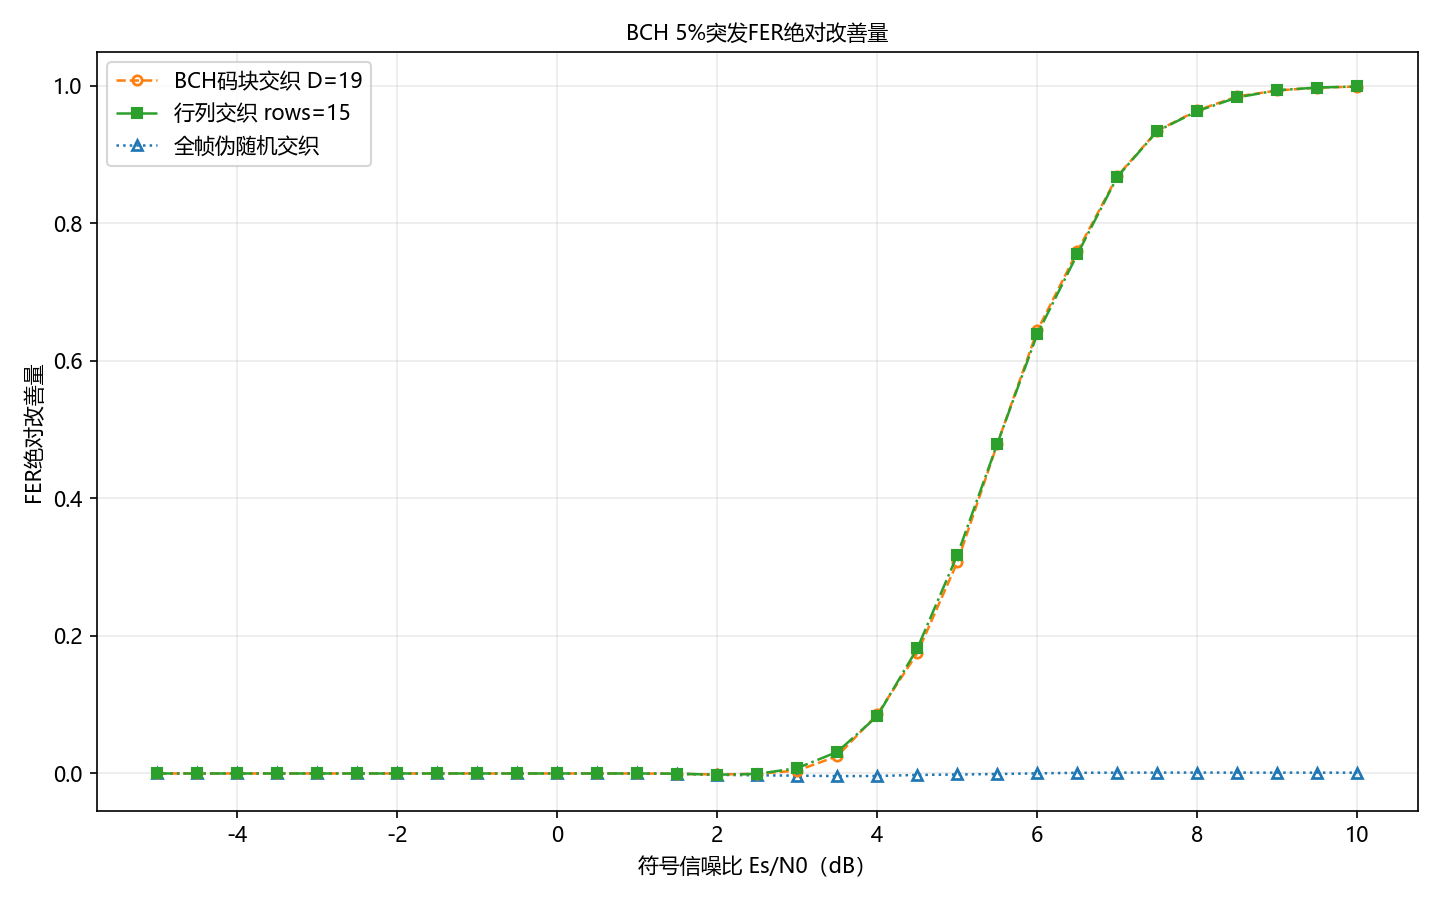
\includegraphics[width=\linewidth]{../Task/Comparison/S7/stage15_scientific_plots/results/bch/11_absoluteFerImprovement/figure.png}\\[-0.2em]
    \small（a）FER绝对改善量
  \end{minipage}\hfill
  \begin{minipage}[t]{0.49\textwidth}
    \centering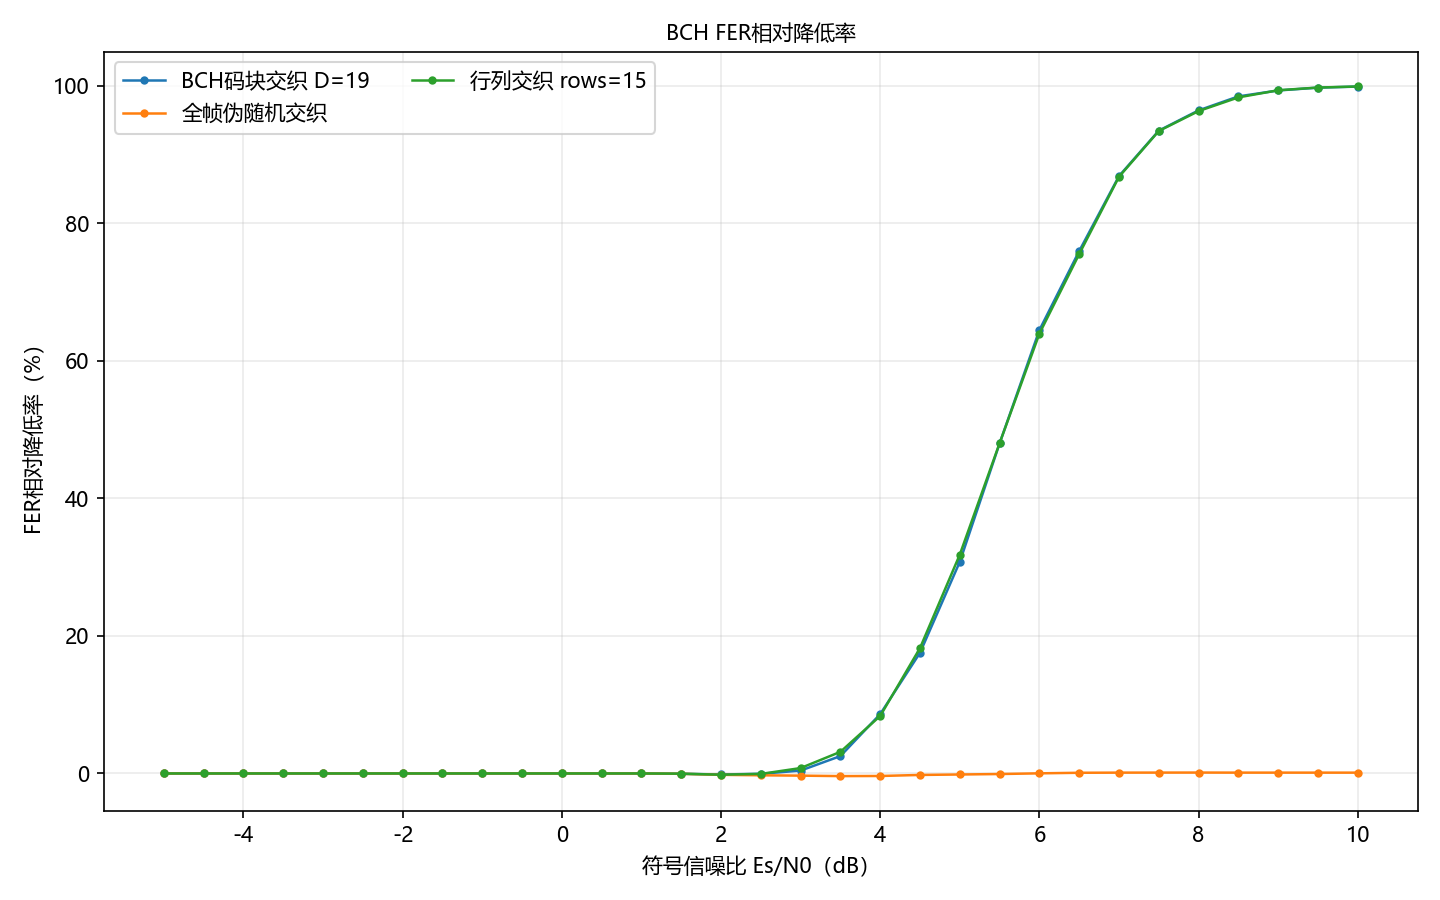
\includegraphics[width=\linewidth]{../Task/Comparison/S7/stage15_scientific_plots/results/bch/12_relativeFerReductionPercent/figure.png}\\[-0.2em]
    \small（b）FER相对降低率
  \end{minipage}
  \caption{5\%突发条件下BCH交织的FER改善}
  \label{fig:s7-bch-fer-gain}
\end{figure}

\subsection{突发位置敏感性}

图\ref{fig:s7-bch-position-statistics}给出六位置平均、最坏和最好FER，图\ref{fig:s7-bch-position-detail}进一步给出推荐行列配置的六条位置曲线与各配置的位置敏感度。无交织和全帧伪随机配置在最好与最坏位置之间存在较大差异；子块结构交织与行列交织在高信噪比区的三类统计量更接近，表明规则映射降低了特定突发起点与子块边界重合所造成的波动。

\begin{figure}[htbp]
  \centering
  \begin{minipage}[t]{0.32\textwidth}
    \centering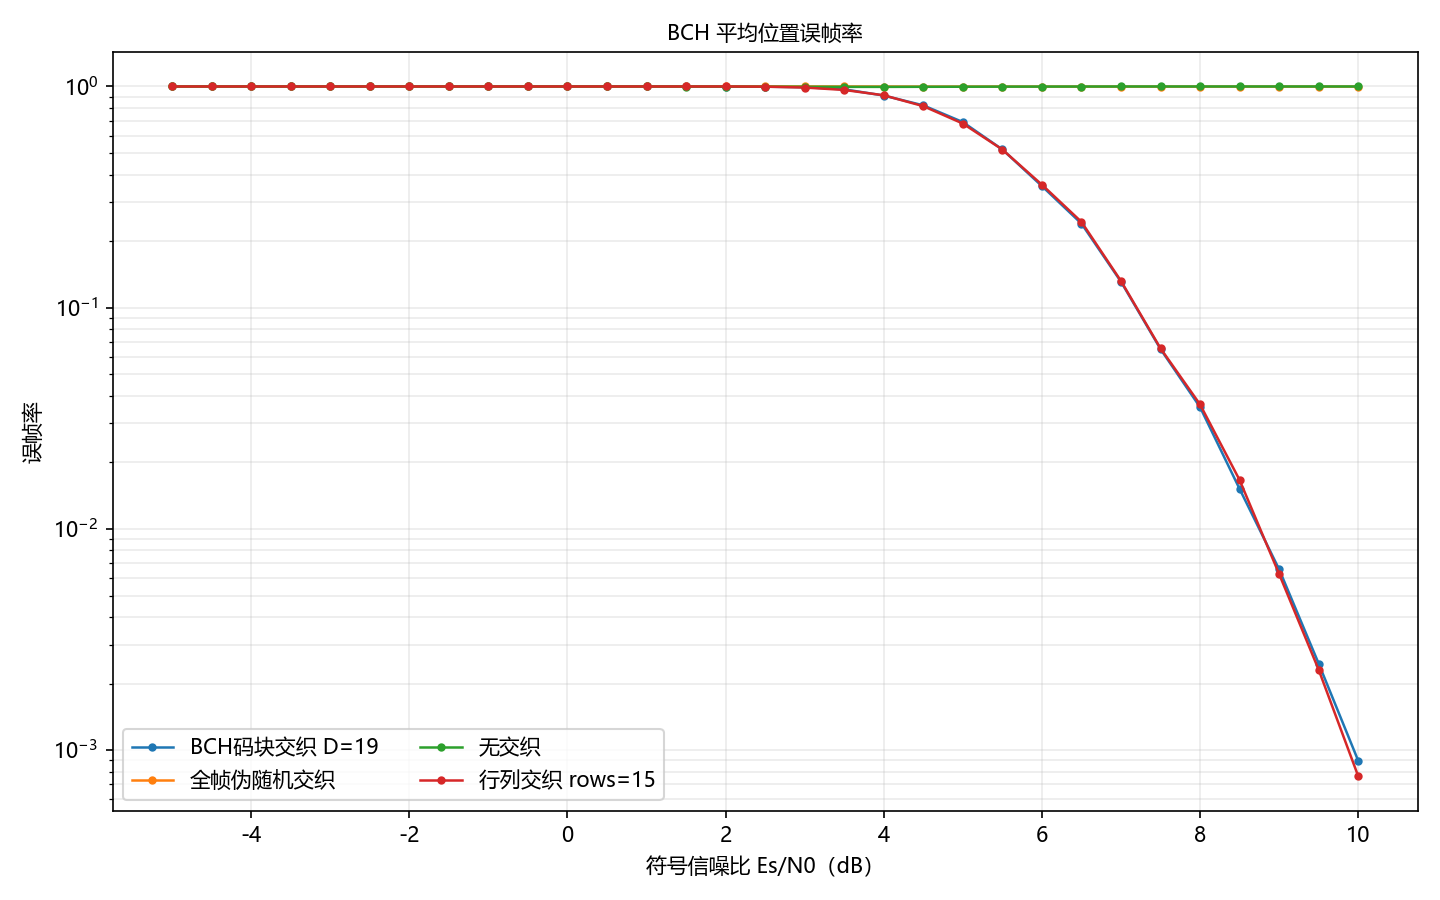
\includegraphics[width=\linewidth]{../Task/Comparison/S7/stage15_scientific_plots/results/bch/07_mean_position_fer/figure.png}\\[-0.2em]\small（a）六位置平均
  \end{minipage}\hfill
  \begin{minipage}[t]{0.32\textwidth}
    \centering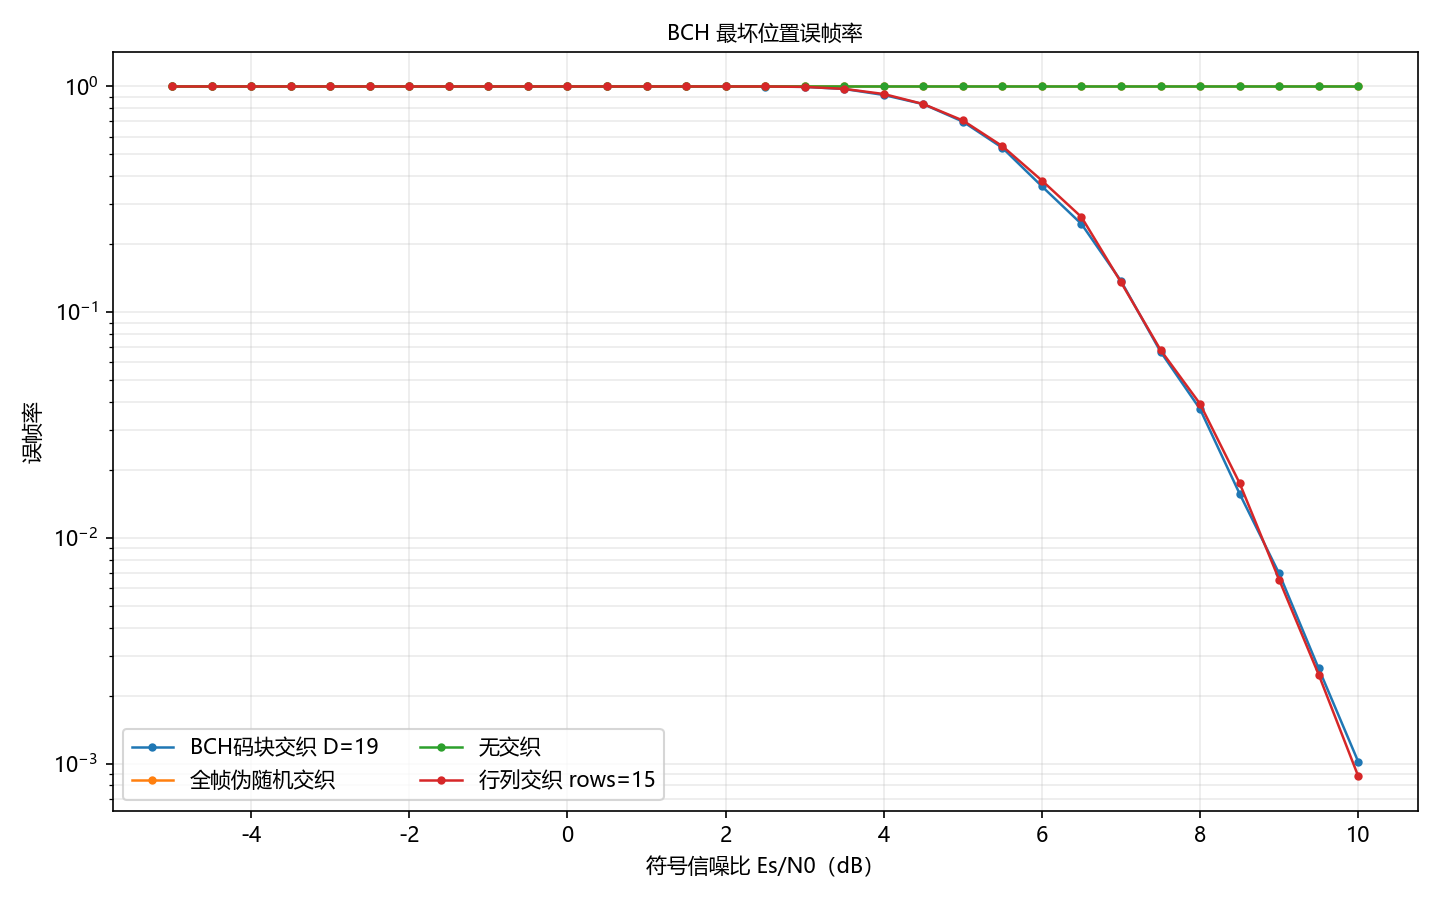
\includegraphics[width=\linewidth]{../Task/Comparison/S7/stage15_scientific_plots/results/bch/08_max_position_fer/figure.png}\\[-0.2em]\small（b）最坏位置
  \end{minipage}\hfill
  \begin{minipage}[t]{0.32\textwidth}
    \centering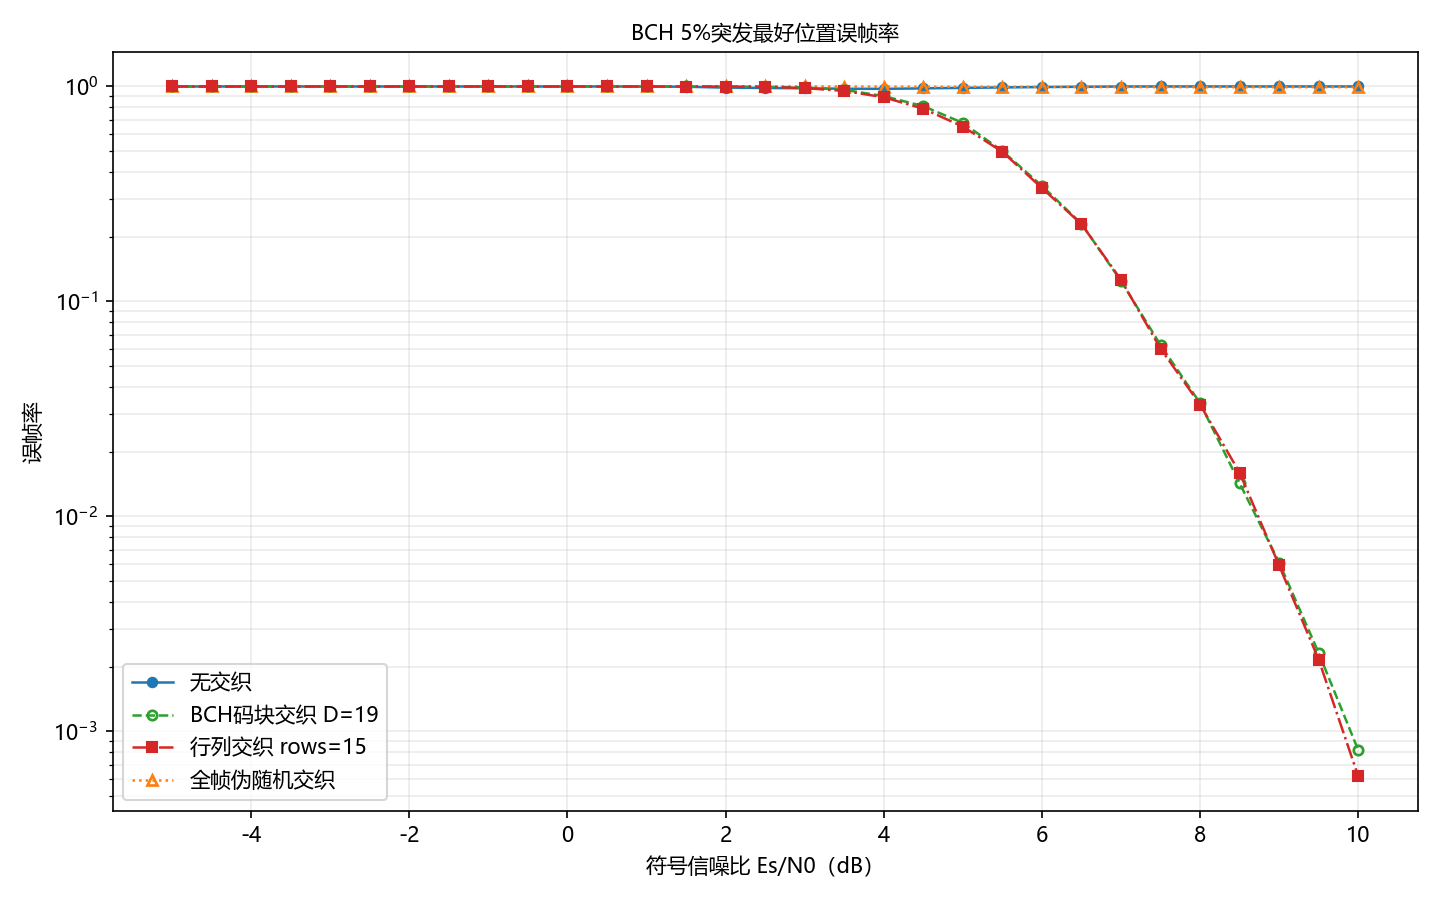
\includegraphics[width=\linewidth]{../Task/Comparison/S7/stage15_scientific_plots/results/bch/09_min_position_fer/figure.png}\\[-0.2em]\small（c）最好位置
  \end{minipage}
  \caption{5\%突发条件下BCH位置统计结果}
  \label{fig:s7-bch-position-statistics}
\end{figure}

\begin{figure}[htbp]
  \centering
  \begin{minipage}[t]{0.49\textwidth}
    \centering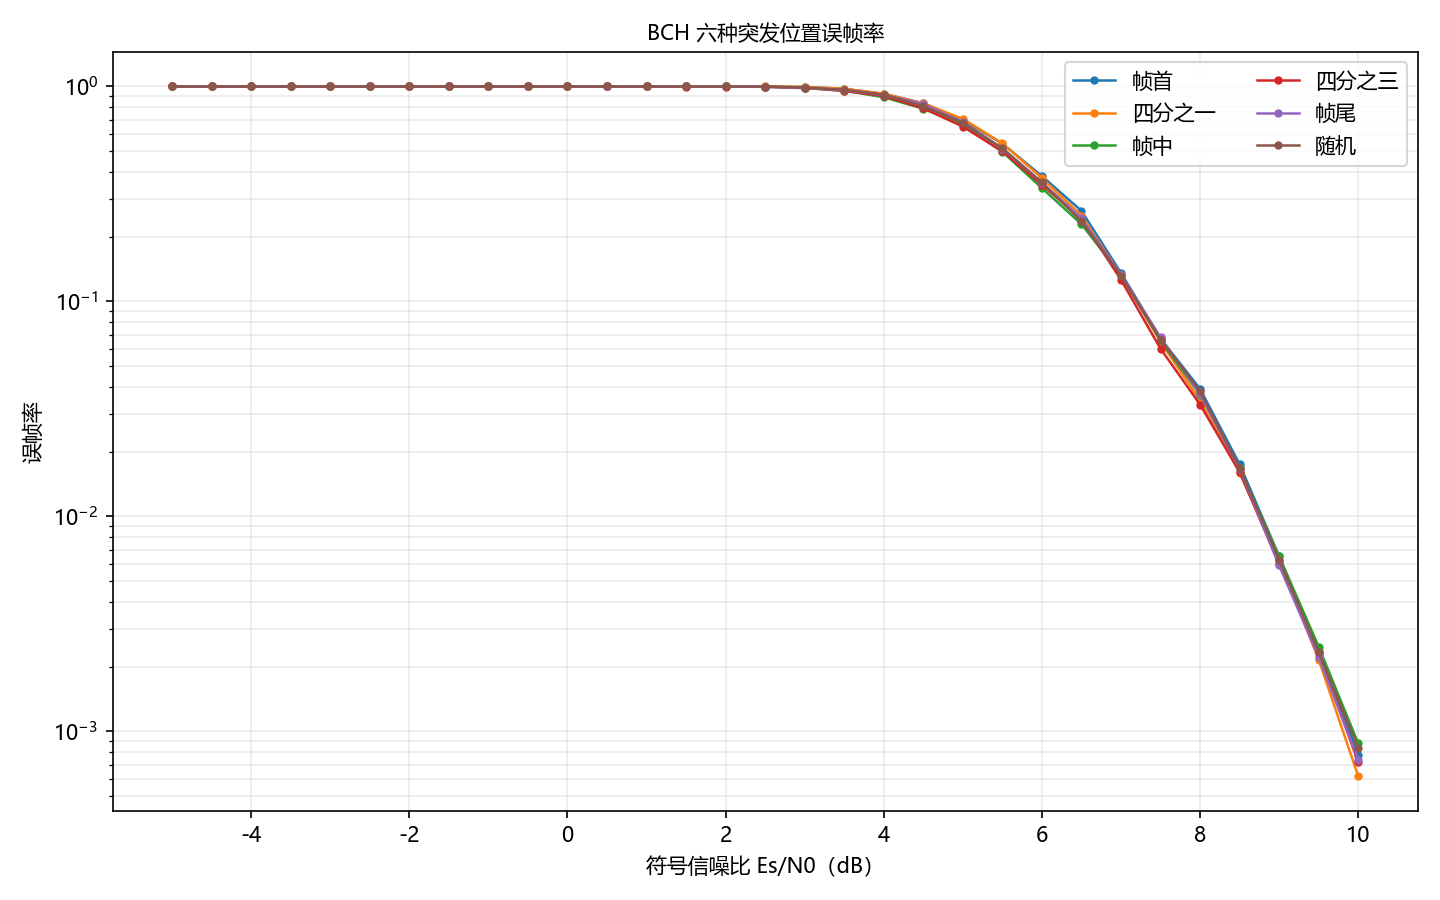
\includegraphics[width=\linewidth]{../Task/Comparison/S7/stage15_scientific_plots/results/bch/06_six_positions_fer/figure.png}\\[-0.2em]\small（a）推荐配置的六位置FER
  \end{minipage}\hfill
  \begin{minipage}[t]{0.49\textwidth}
    \centering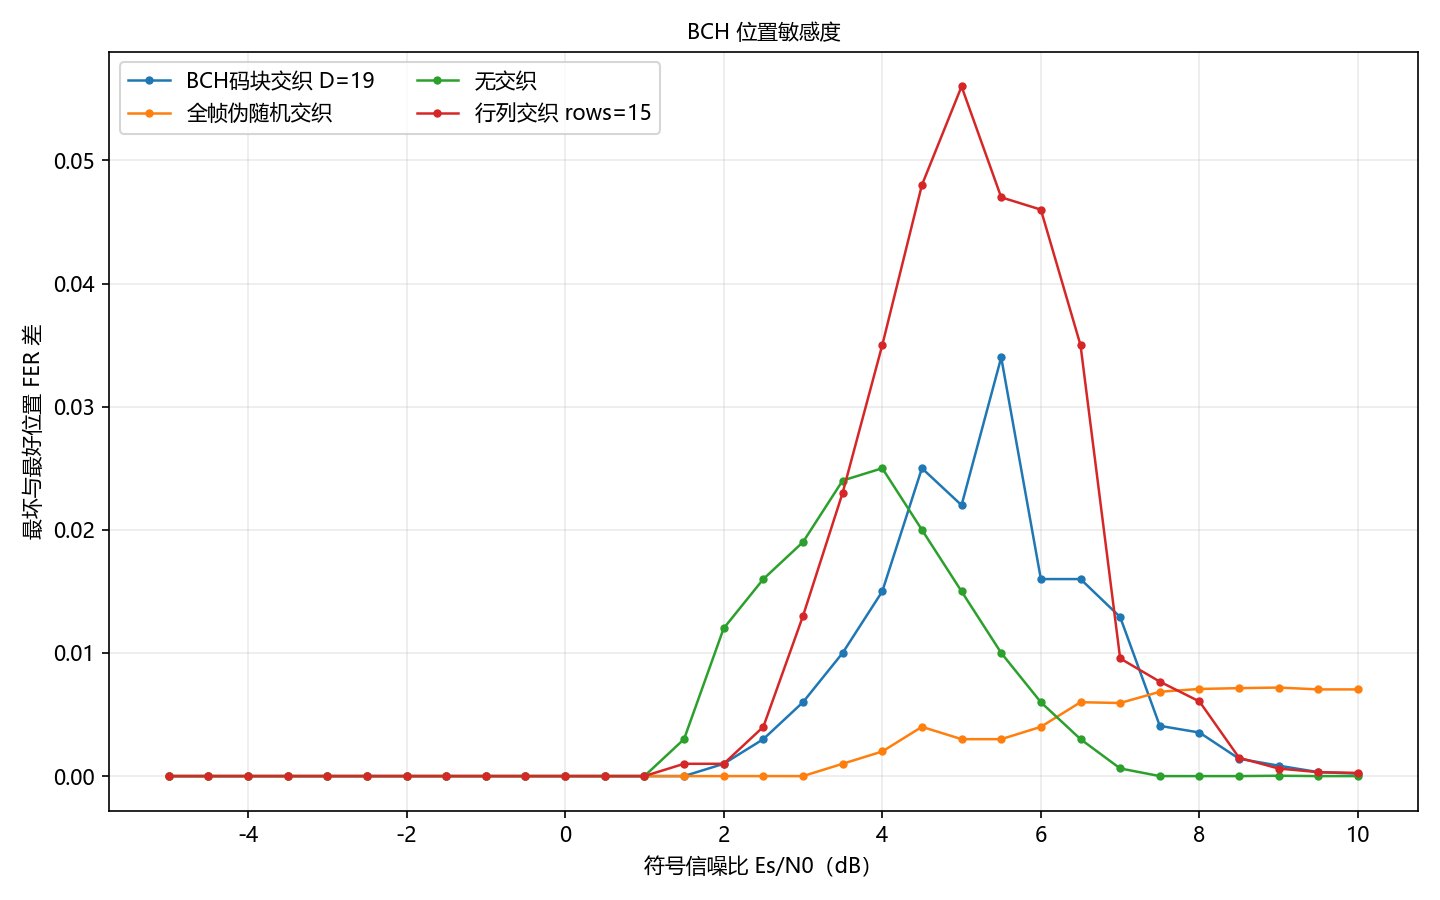
\includegraphics[width=\linewidth]{../Task/Comparison/S7/stage15_scientific_plots/results/bch/10_position_sensitivity/figure.png}\\[-0.2em]\small（b）最坏与最好位置FER差
  \end{minipage}
  \caption{5\%突发条件下BCH突发位置敏感性}
  \label{fig:s7-bch-position-detail}
\end{figure}

全起点扫描为六位置结果提供了更细粒度的验证。图\ref{fig:s7-bch-heatmaps}中，2\%与5\%热力图均保留每个已测试起点的原始FER，不对未测试位置插值。2\%条件下不同起点的差异更容易分辨；5\%条件下，规则结构交织仍保持较低的高工作点FER，而无交织与全帧伪随机配置在多数起点上维持高错误率。该结果说明六个代表位置没有掩盖主要的结构性差异。

\begin{figure}[htbp]
  \centering
  \begin{minipage}[t]{0.49\textwidth}
    \centering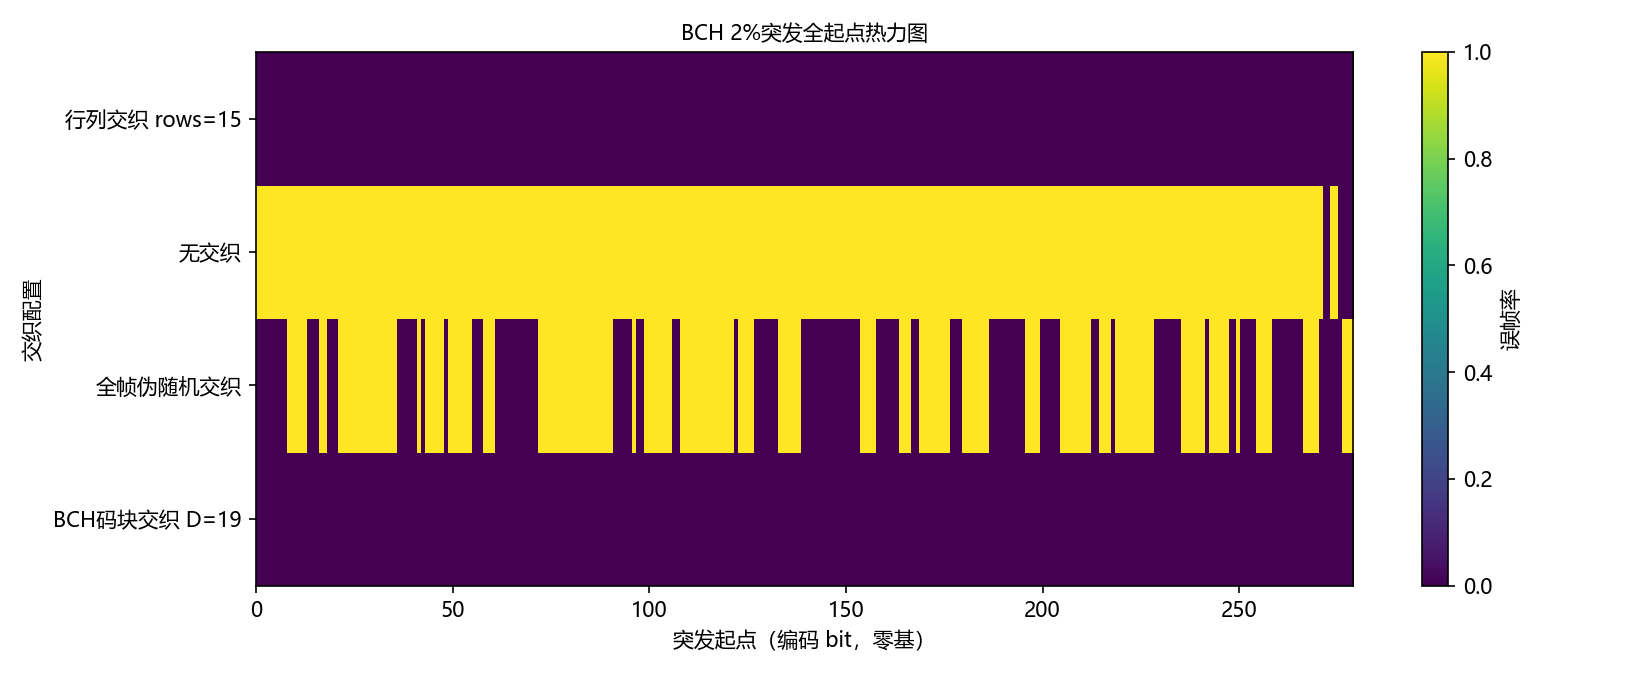
\includegraphics[width=\linewidth]{../Task/Comparison/S7/stage15_scientific_plots/results/bch/21_all_start_heatmap_2_percent/figure.png}\\[-0.2em]\small（a）2\%突发
  \end{minipage}\hfill
  \begin{minipage}[t]{0.49\textwidth}
    \centering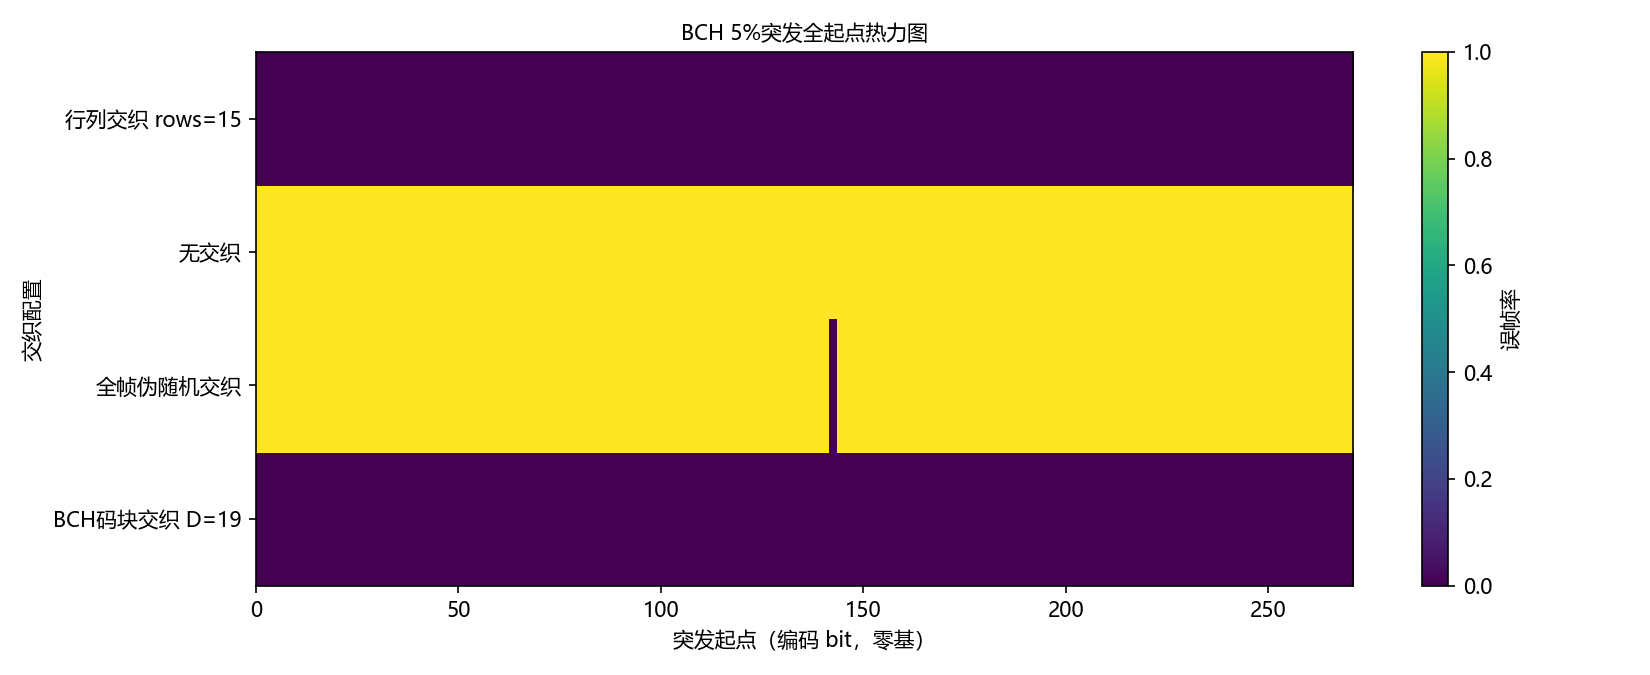
\includegraphics[width=\linewidth]{../Task/Comparison/S7/stage15_scientific_plots/results/bch/22_all_start_heatmap_5_percent/figure.png}\\[-0.2em]\small（b）5\%突发
  \end{minipage}
  \caption{BCH高工作点全起点FER热力图}
  \label{fig:s7-bch-heatmaps}
\end{figure}

\subsection{错误跨BCH子块分散机制}

分块BCH的机理可以由受影响子块数与单块最大错误数共同解释。无交织时，连续突发集中落入少量15 bit子块，局部子块可能同时包含多个错误，超过BCH(15,11,1)的单比特保证纠错范围。交织后，同一连续异常经逆置换分散到更多子块，使单个子块内的最大错误数下降，更多子块处于原有单比特可纠正范围。交织没有改变BCH码本或理论纠错能力，而是改善了原有局部纠错能力的利用方式。

图\ref{fig:s7-bch-mechanism}给出行列交织在5\%条件下的两项诊断量。$E_s/N_0=10$ dB时，14 bit突发平均影响约14.0003个子块，单块最大错误数为2。表\ref{tab:s7-bch-mechanism}进一步与其他配置对照：无交织平均只涉及1.4778个子块，但单块最大错误数达到15；全帧伪随机交织涉及约10.7210个子块，单块最大错误数为4；两种规则结构交织均把错误扩展到约14个子块，并把最大值压低至2。该分布变化与表\ref{tab:s7-bch-fer-improvement}中的FER差异一致。

\begin{figure}[htbp]
  \centering
  \begin{minipage}[t]{0.49\textwidth}
    \centering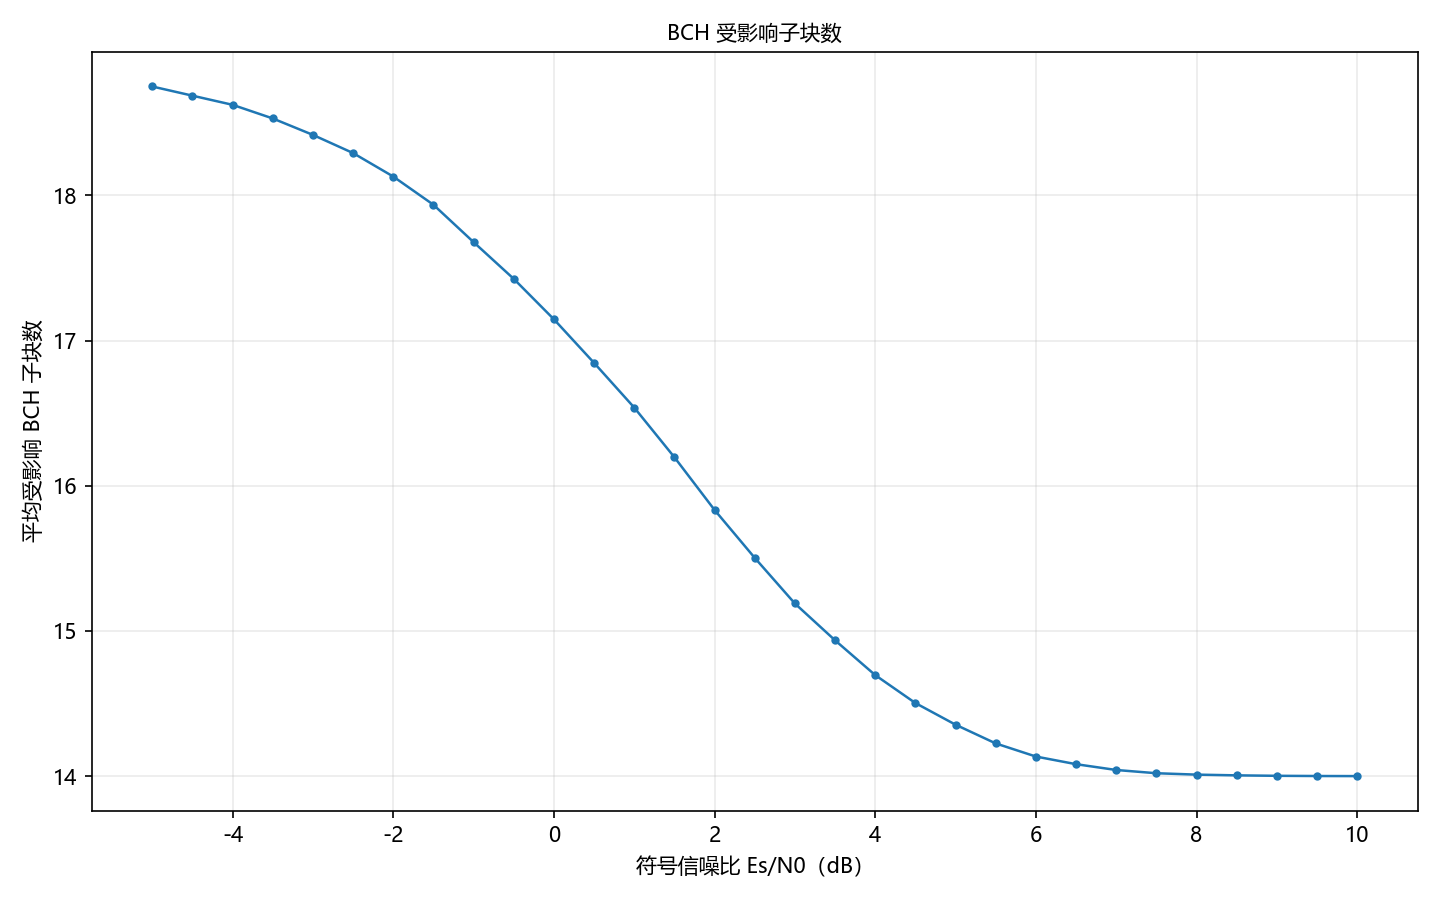
\includegraphics[width=\linewidth]{../Task/Comparison/S7/stage15_scientific_plots/results/bch/14_affected_bch_blocks/figure.png}\\[-0.2em]\small（a）平均受影响子块数
  \end{minipage}\hfill
  \begin{minipage}[t]{0.49\textwidth}
    \centering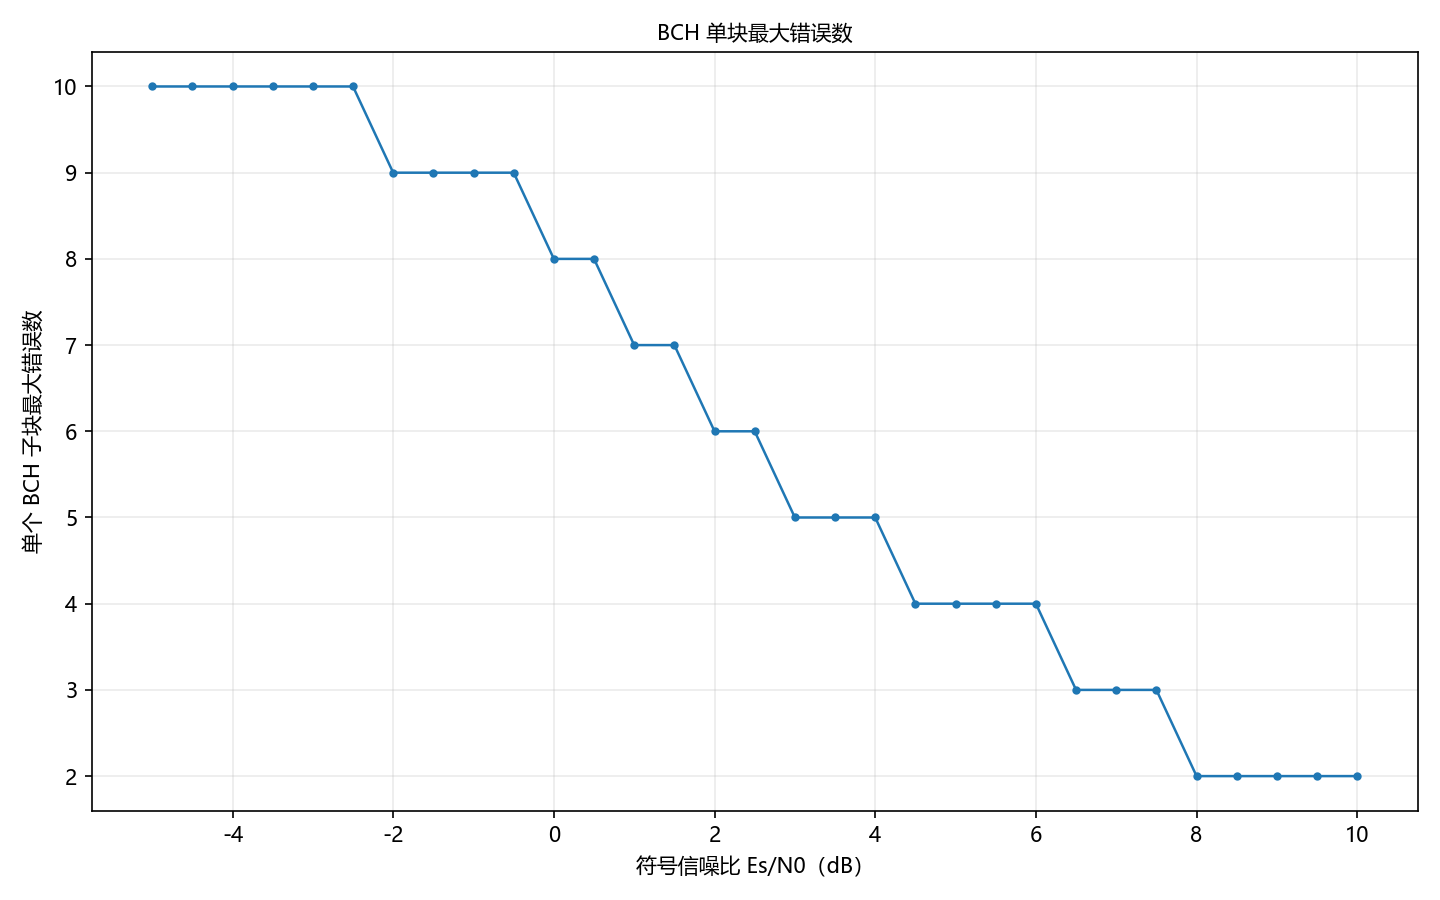
\includegraphics[width=\linewidth]{../Task/Comparison/S7/stage15_scientific_plots/results/bch/15_max_errors_per_block/figure.png}\\[-0.2em]\small（b）单块最大错误数
  \end{minipage}
  \caption{5\%突发条件下BCH错误分散机理证据}
  \label{fig:s7-bch-mechanism}
\end{figure}

\begin{table}[htbp]
  \centering
  \caption{BCH错误分散机制（$E_s/N_0=10$ dB，5\%突发）}
  \label{tab:s7-bch-mechanism}
  \small
  \begin{tabular}{lrrrr}
    \toprule
    配置 & 受影响子块均值 & 单块最大错误数 & 纠正子块均值 & 平均FER \\
    \midrule
    无交织 & 1.4778 & 15 & 0.5222 & 1 \\
    子块结构$D=19$ & 14.0003 & 2 & 14.0003 & $8.97\times10^{-4}$ \\
    行列$R=15$ & 14.0003 & 2 & 14.0003 & $7.63\times10^{-4}$ \\
    全帧伪随机 & 10.7210 & 4 & 8.9673 & 0.998823 \\
    \bottomrule
  \end{tabular}
\end{table}

\subsection{缓冲需求与软件处理时间}

三种BCH交织配置均需285 bit结构缓存，见图\ref{fig:s7-bch-buffer}。仅按2\%和5\%正式仿真数据进行帧数加权后，无交织、子块结构、行列和全帧伪随机配置的软件交织CPU时间分别为328.4、324.9、325.3和325.1 ns/帧；去交织时间分别为310.5、329.9、322.6和324.6 ns/帧。交织函数本身的时间差小于十纳秒量级，译码CPU时间约为$8.42\sim9.00~\mu$s/帧。上述数值是\texttt{steady\_clock}包围软件函数得到的处理时间，不包括编码、调制、信道，也不能直接换算为硬件时延。

\begin{figure}[htbp]
  \centering
  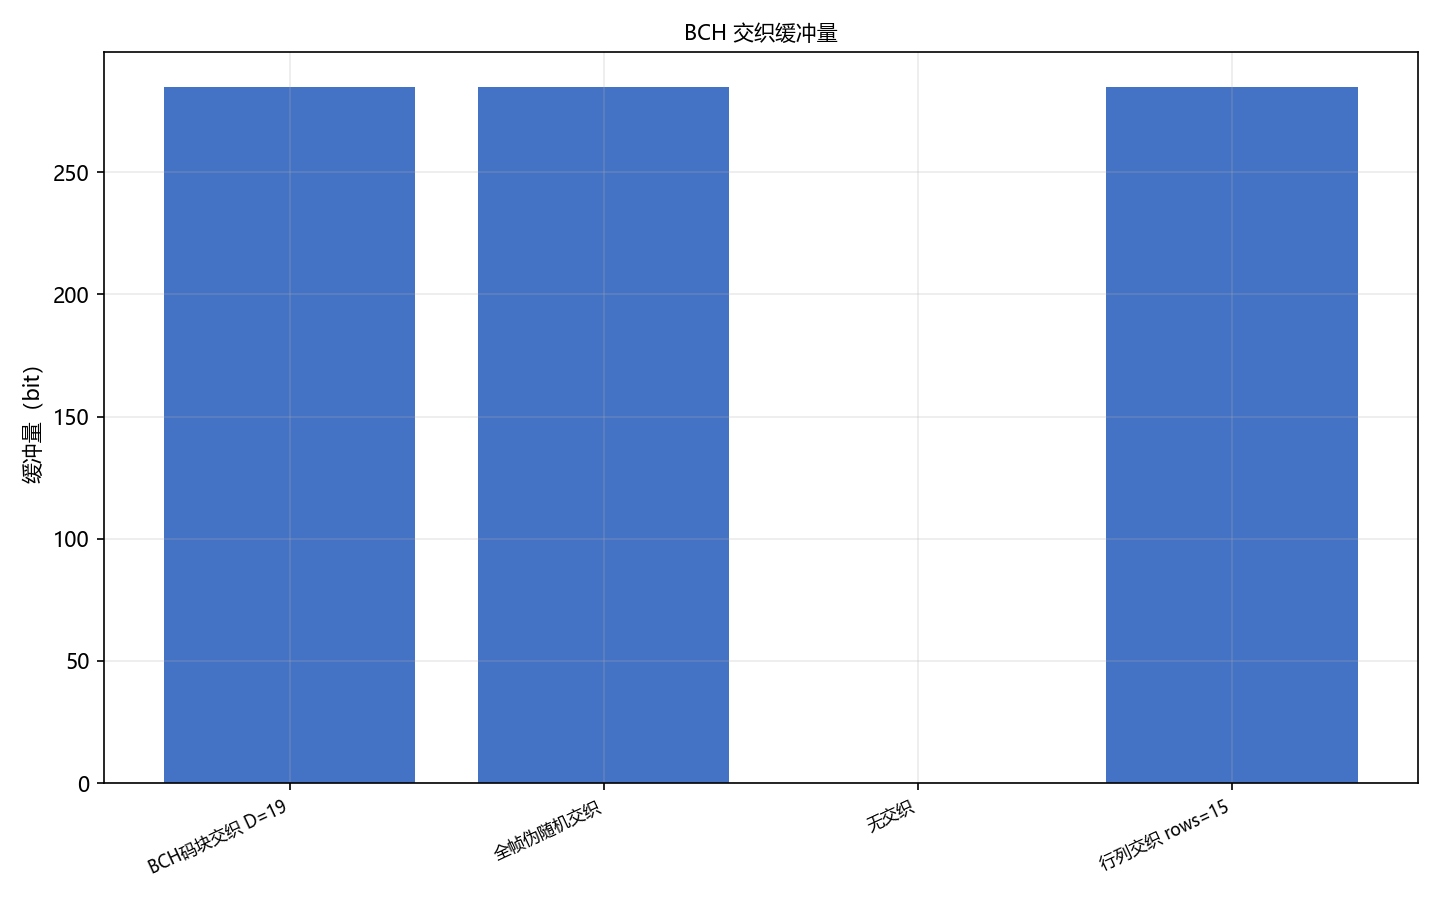
\includegraphics[width=0.88\textwidth]{../Task/Comparison/S7/stage15_scientific_plots/results/bch/19_bufferBits/figure.png}
  \caption{BCH交织配置的结构缓存量}
  \label{fig:s7-bch-buffer}
\end{figure}

\section{卷积码交织抗突发错误结果}

\subsection{不同交织配置总体BER与FER}

图\ref{fig:s7-cc-burst-fer}给出2\%和5\%突发下卷积码FER。图中的LDPC曲线是无交织、无突发AWGN近码率基线，只用于高速编码方案参考，不表示LDPC经历对应的突发错误条件。2\%条件下，局部伪随机Pseudo128和短深度$D=8$在高信噪比区降低了平均FER；5\%条件下，各卷积码配置在当前$E_s/N_0$上限附近仍接近FER饱和区，因而不能从本测试范围给出稳定的低FER工作点。

\begin{figure}[htbp]
  \centering
  \begin{minipage}[t]{0.49\textwidth}
    \centering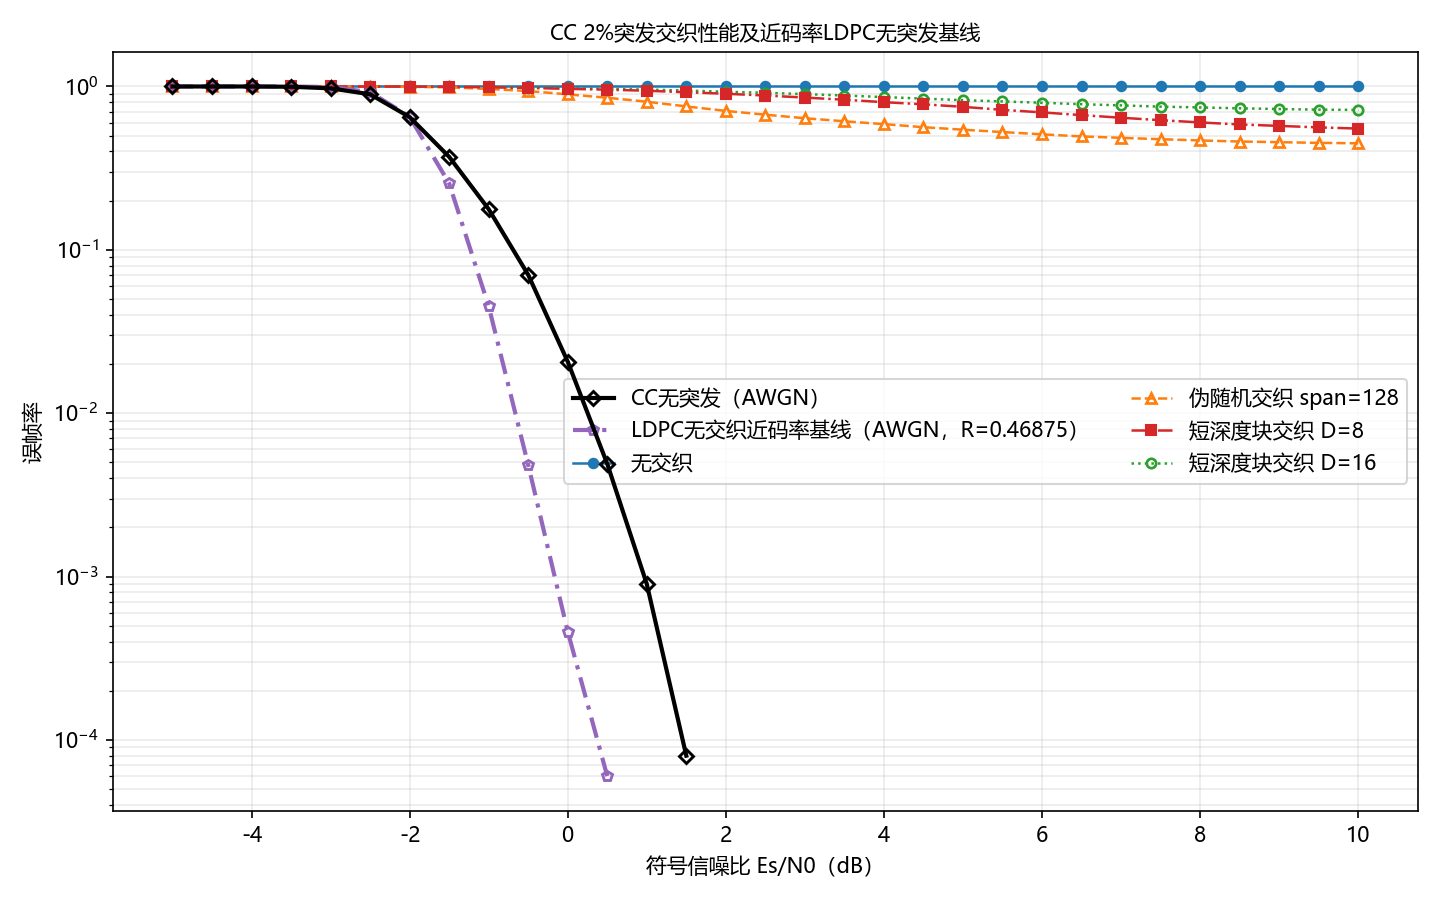
\includegraphics[width=\linewidth]{../Task/Comparison/S7/stage15_scientific_plots/results/cc/03_burst_2_fer/figure.png}\\[-0.2em]\small（a）2\%突发
  \end{minipage}\hfill
  \begin{minipage}[t]{0.49\textwidth}
    \centering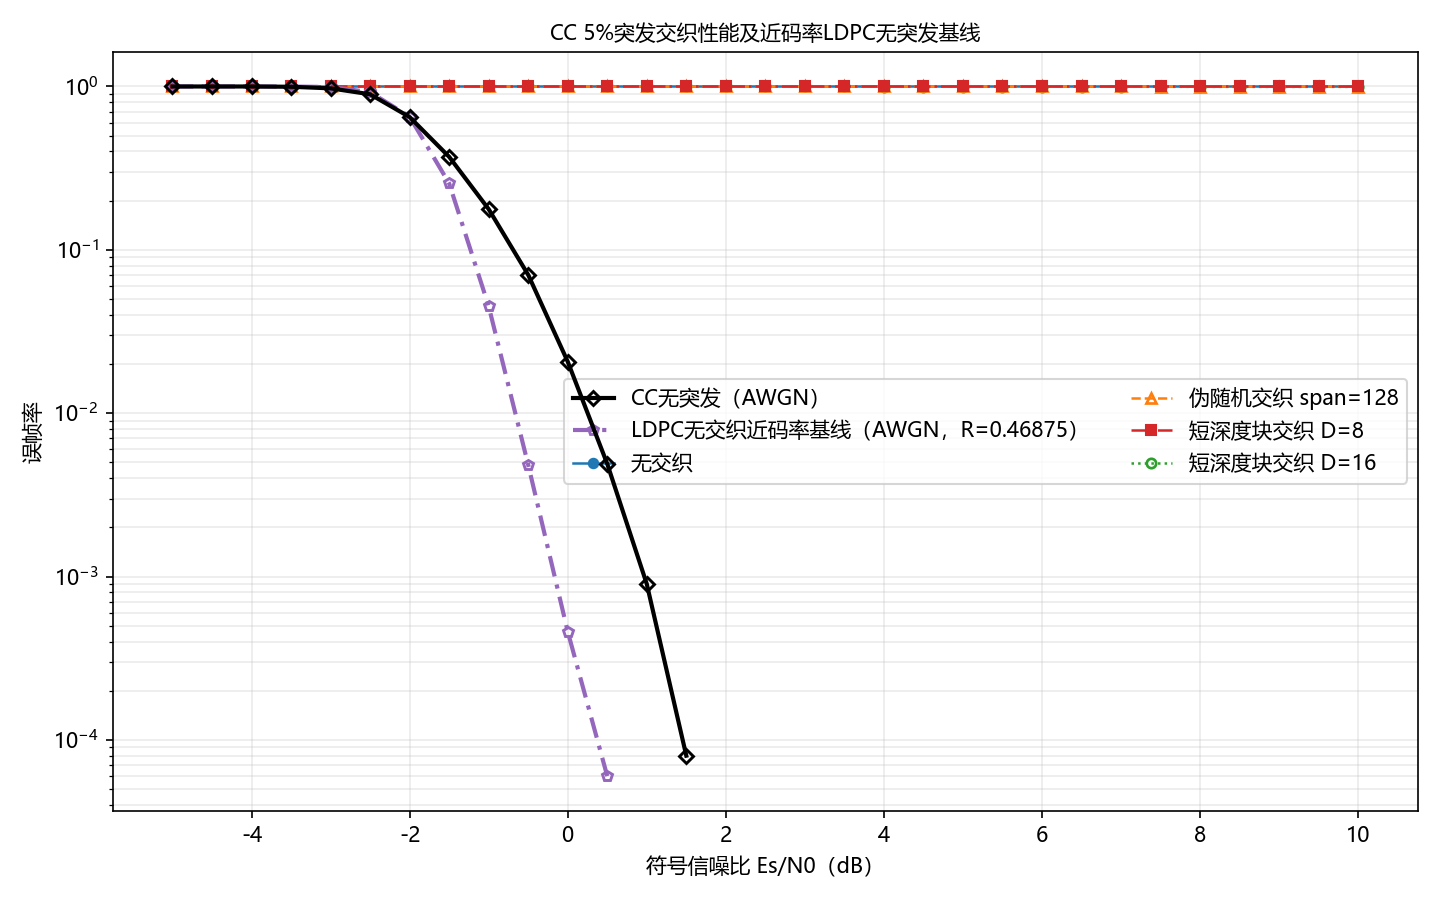
\includegraphics[width=\linewidth]{../Task/Comparison/S7/stage15_scientific_plots/results/cc/04_burst_5_fer/figure.png}\\[-0.2em]\small（b）5\%突发
  \end{minipage}
  \caption{卷积码在两档突发长度下的误帧率。LDPC曲线为无突发AWGN近码率基线，不表示LDPC经历突发错误}
  \label{fig:s7-cc-burst-fer}
\end{figure}

表\ref{tab:s7-cc-fer-improvement}给出$10$ dB定量结果。2\%条件下，无交织FER为1，$D=8$、Pseudo128和$D=16$的六位置平均FER分别为0.552654、0.448905和0.718629，相对无交织分别下降44.73\%、55.11\%和28.14\%。5\%条件下，三种交织配置的平均FER均不低于0.9945，最坏位置FER均为1。该结果支持交织对较短突发具有可观测收益，同时也限定了本卷积码配置在31 bit连续异常下的能力边界。

\begin{table}[htbp]
  \centering
  \caption{卷积码代表性FER改善（$E_s/N_0=10$ dB）}
  \label{tab:s7-cc-fer-improvement}
  \footnotesize
  \begin{tabular}{clrrrr}
    \toprule
    突发 & 配置 & 平均FER & 最坏FER & 最好FER & 相对降低/\% \\
    \midrule
    2\% & 无交织 & 1 & 1 & 1 & 0 \\
    2\% & 短深度$D=8$ & 0.552654 & 0.85 & 0.063805 & 44.7346 \\
    2\% & Pseudo128 & 0.448905 & 0.84 & 0.004165 & 55.1095 \\
    2\% & 短深度$D=16$ & 0.718629 & 1 & 0.498 & 28.1371 \\
    5\% & 无交织 & 1 & 1 & 1 & 0 \\
    5\% & 短深度$D=8$ & 1 & 1 & 1 & 0 \\
    5\% & Pseudo128 & 0.999667 & 1 & 0.998 & 0.0333 \\
    5\% & 短深度$D=16$ & 0.994500 & 1 & 0.984 & 0.5500 \\
    \bottomrule
  \end{tabular}
\end{table}

\subsection{两档突发长度的影响}

12 bit突发与31 bit突发呈现出不同的可恢复区间。2\%条件下，Pseudo128和$D=8$在$10$ dB处分别把平均FER降至0.448905和0.552654，最好位置FER分别达到0.004165和0.063805，说明较短连续异常经逆置换后能够减少对相邻路径度量的集中作用。然而两者最坏位置FER仍为0.84和0.85，位置依赖没有消失。$D=16$在相同工作点的平均FER为0.718629，表明更大规则块深度并不自动带来更低FER。

31 bit突发覆盖约15.5个母码输出对。在当前最高$E_s/N_0$下，$D=8$平均FER仍为1，Pseudo128和$D=16$分别为0.999667和0.994500，且所有配置最坏位置FER均为1。AWGN继续降低时，突发造成的连续异常仍足以维持路径竞争错误，形成高FER平台。该数据边界意味着卷积码交织的工程建议主要由2\%条件支撑；5\%结果用于界定当前配置的不足，不能用极小的平均差值声称已经形成稳定改善。

FER与BER反映的侧面并不完全相同。图\ref{fig:s7-cc-ber}显示5\%条件下各配置的BER曲线；在$10$ dB时，无交织、$D=8$、Pseudo128和$D=16$的平均BER分别为0.016864、0.089080、0.069413和0.129994。此时交织后的FER仍接近1，且BER没有相对无交织改善，因此不能只依据局部路径分散机理推断所有误码指标都会同步下降。正式结论以实测FER与BER分别表述。

\begin{figure}[htbp]
  \centering
  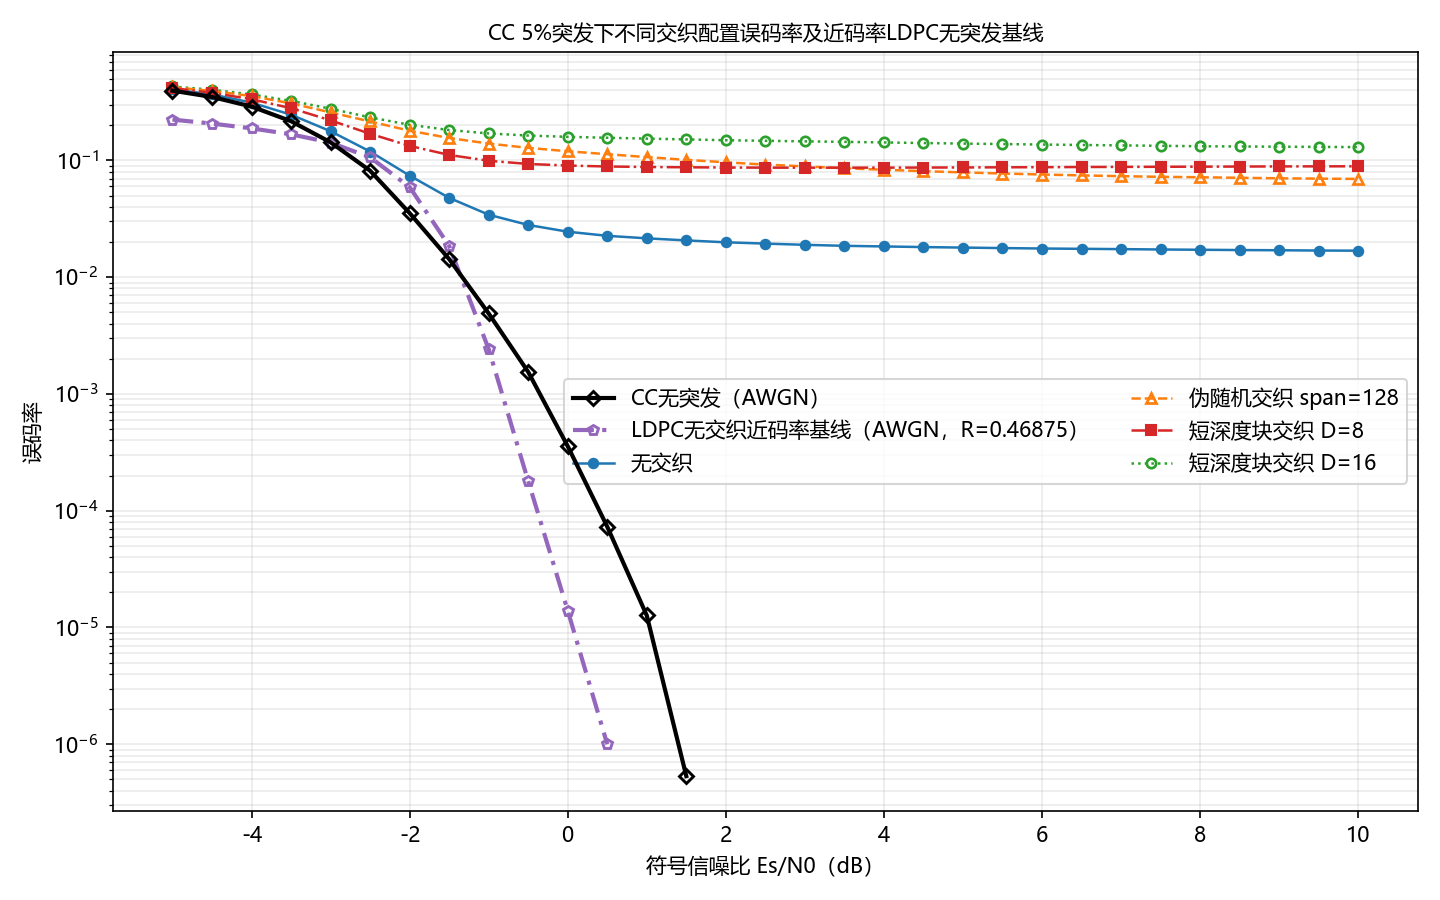
\includegraphics[width=0.88\textwidth]{../Task/Comparison/S7/stage15_scientific_plots/results/cc/02_methods_ber/figure.png}
  \caption{5\%突发条件下卷积码不同交织配置的误码率。LDPC曲线为无突发AWGN近码率基线}
  \label{fig:s7-cc-ber}
\end{figure}

\subsection{突发位置敏感性}

图\ref{fig:s7-cc-position-statistics}给出5\%条件下的平均、最坏和最好位置FER。由于多数曲线处于FER饱和区，三类统计量的间距有限；图\ref{fig:s7-cc-position-detail}中的六位置曲线和敏感度仍表明，2\%较短突发下不同起点会显著改变局部路径竞争，尤其在高信噪比区更易形成可见差异。位置敏感性必须与突发比例和工作点联合解释，不能只用单一最坏位置替代完整统计。

\begin{figure}[htbp]
  \centering
  \begin{minipage}[t]{0.32\textwidth}
    \centering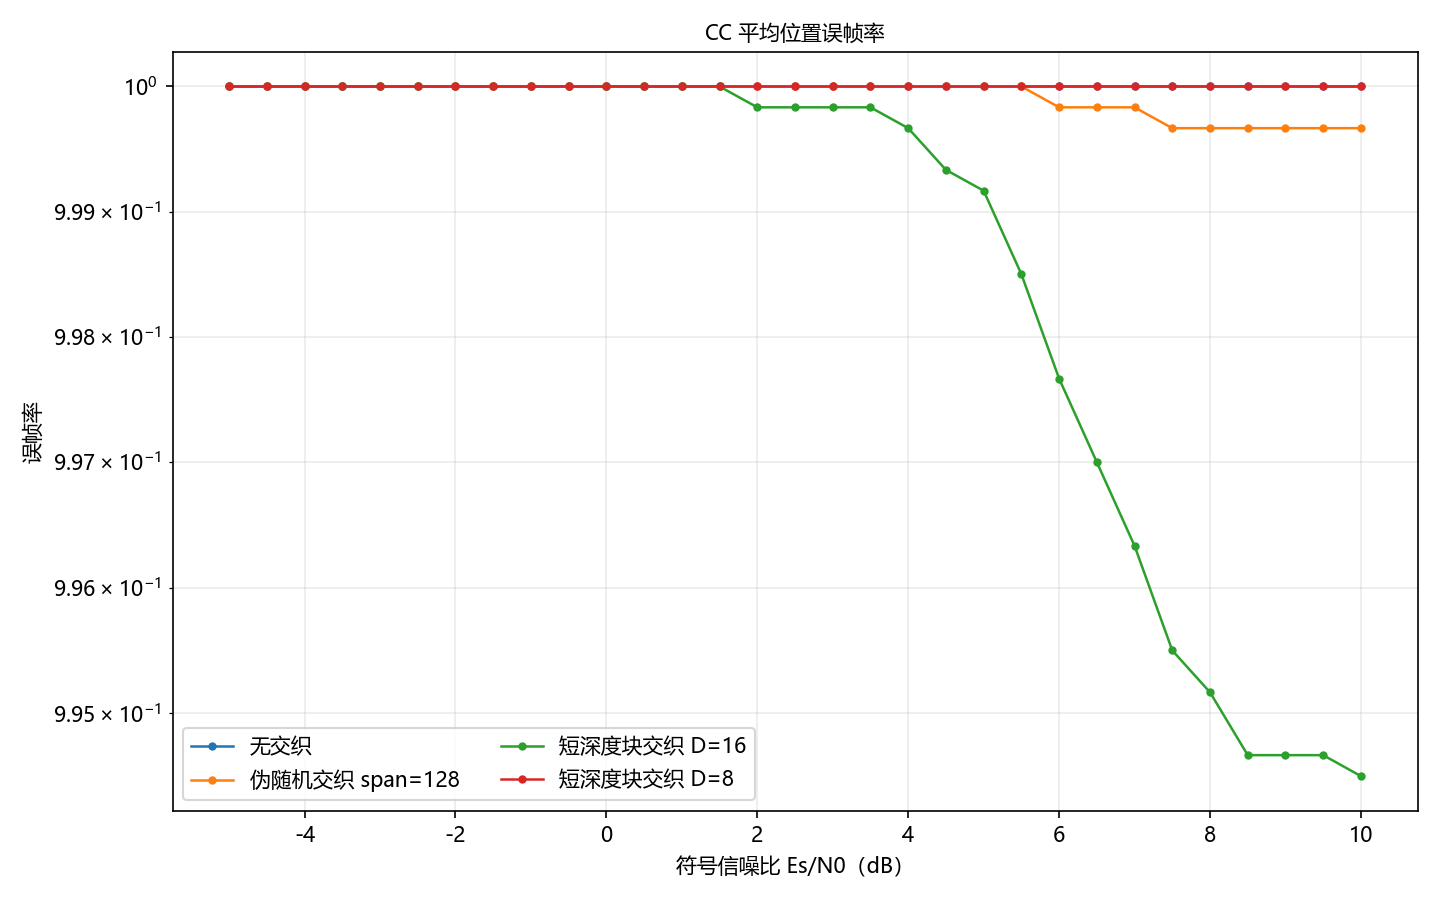
\includegraphics[width=\linewidth]{../Task/Comparison/S7/stage15_scientific_plots/results/cc/07_mean_position_fer/figure.png}\\[-0.2em]\small（a）六位置平均
  \end{minipage}\hfill
  \begin{minipage}[t]{0.32\textwidth}
    \centering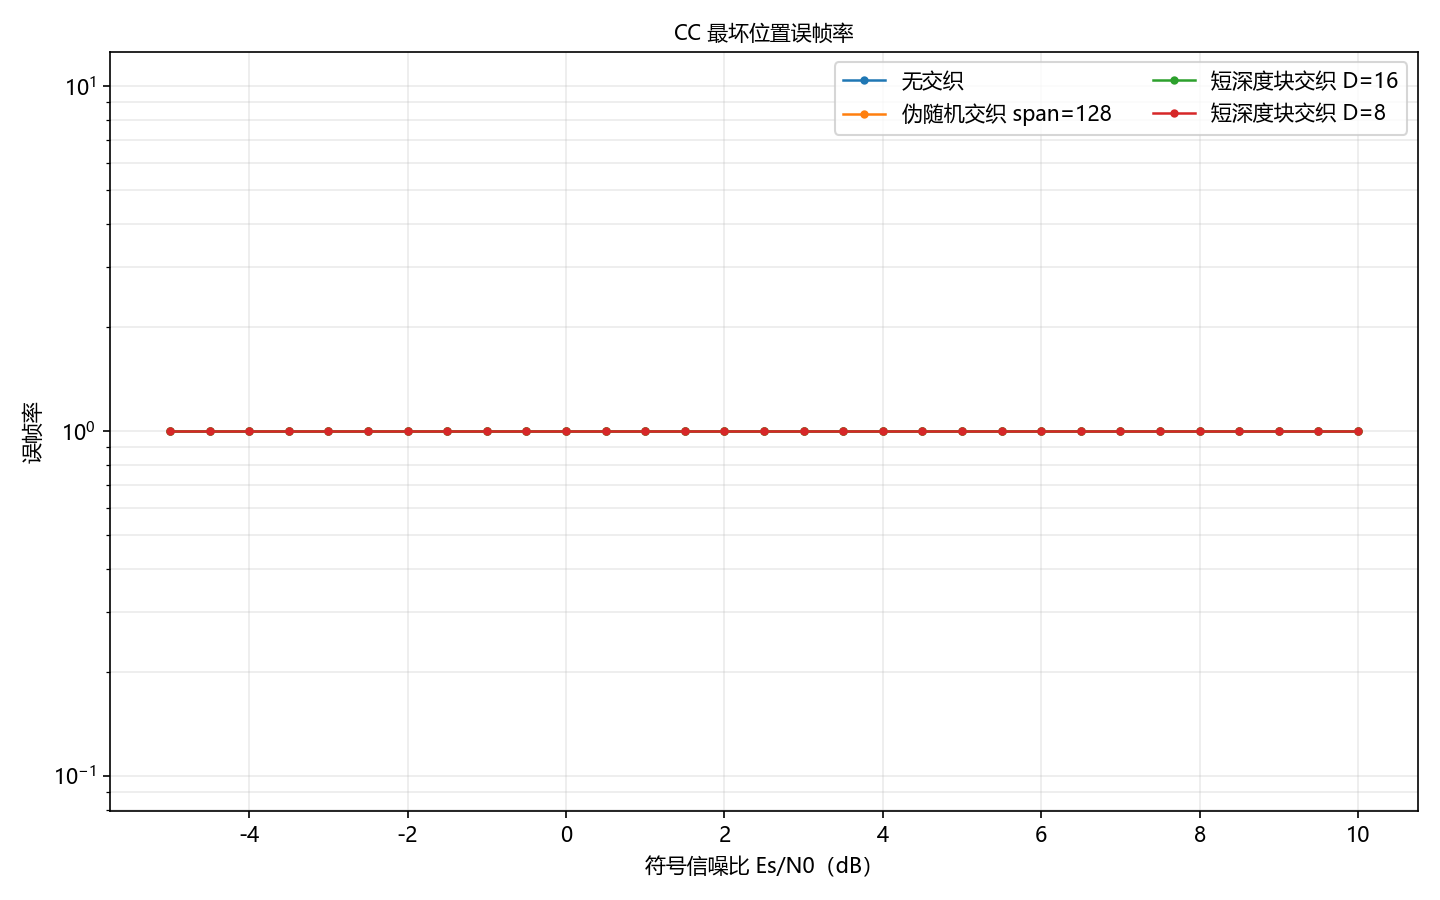
\includegraphics[width=\linewidth]{../Task/Comparison/S7/stage15_scientific_plots/results/cc/08_max_position_fer/figure.png}\\[-0.2em]\small（b）最坏位置
  \end{minipage}\hfill
  \begin{minipage}[t]{0.32\textwidth}
    \centering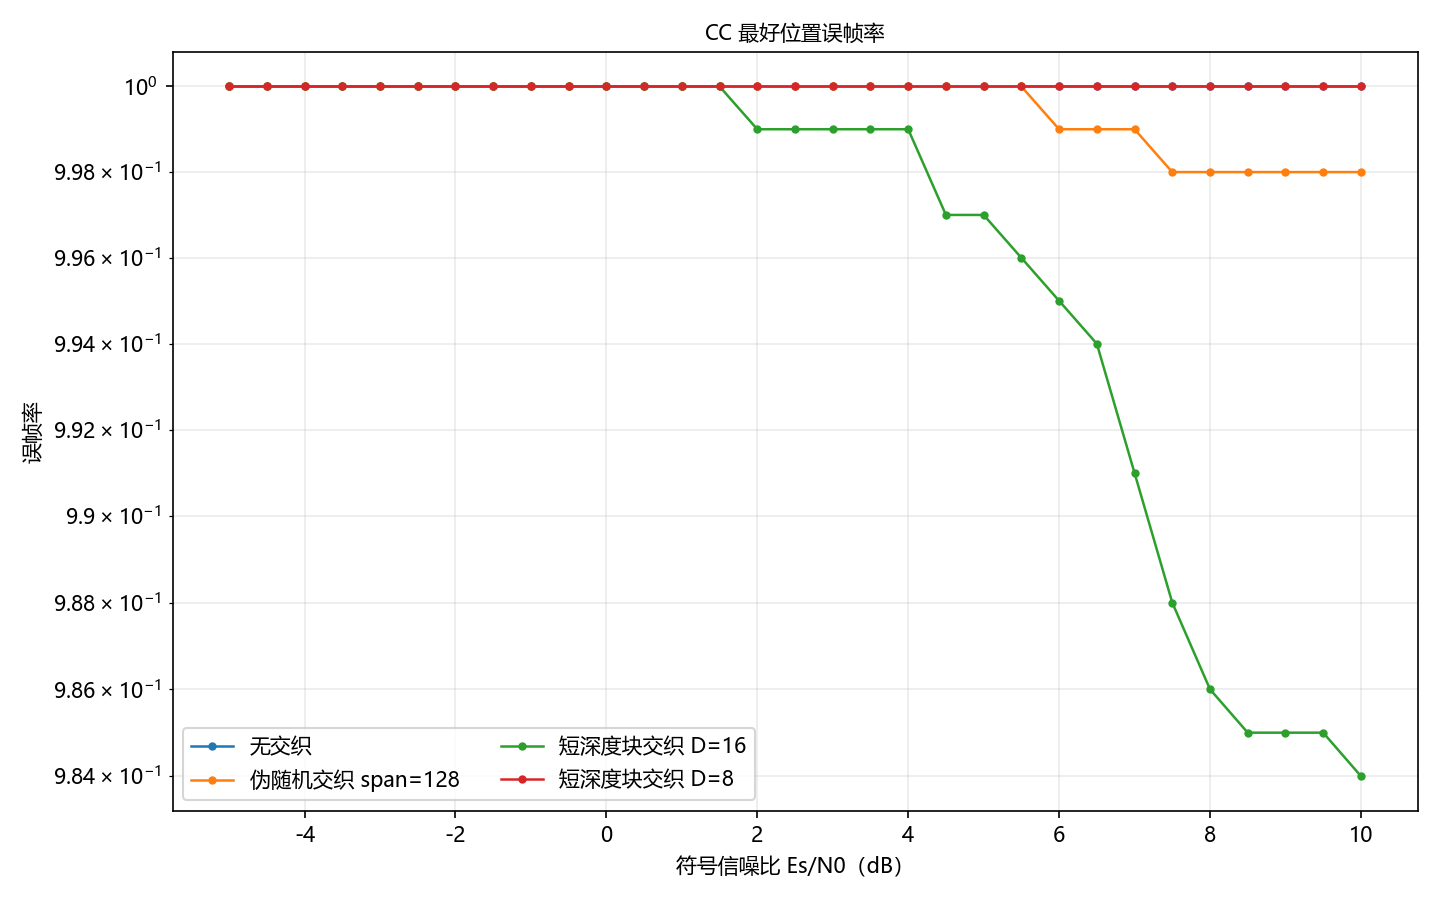
\includegraphics[width=\linewidth]{../Task/Comparison/S7/stage15_scientific_plots/results/cc/09_min_position_fer/figure.png}\\[-0.2em]\small（c）最好位置
  \end{minipage}
  \caption{5\%突发条件下卷积码位置统计结果}
  \label{fig:s7-cc-position-statistics}
\end{figure}

\begin{figure}[htbp]
  \centering
  \begin{minipage}[t]{0.49\textwidth}
    \centering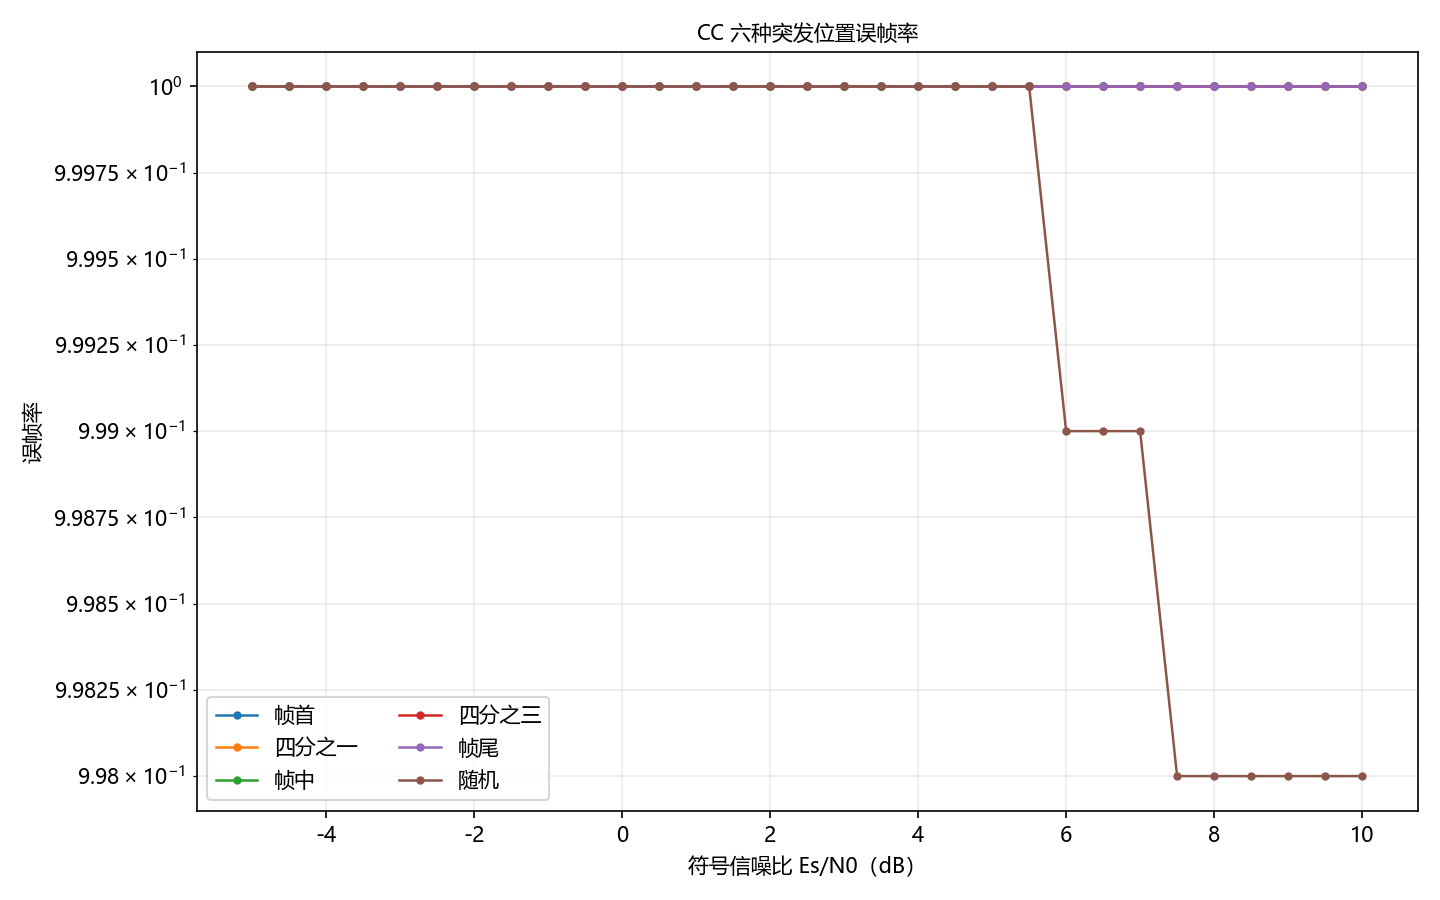
\includegraphics[width=\linewidth]{../Task/Comparison/S7/stage15_scientific_plots/results/cc/06_six_positions_fer/figure.png}\\[-0.2em]\small（a）六位置FER
  \end{minipage}\hfill
  \begin{minipage}[t]{0.49\textwidth}
    \centering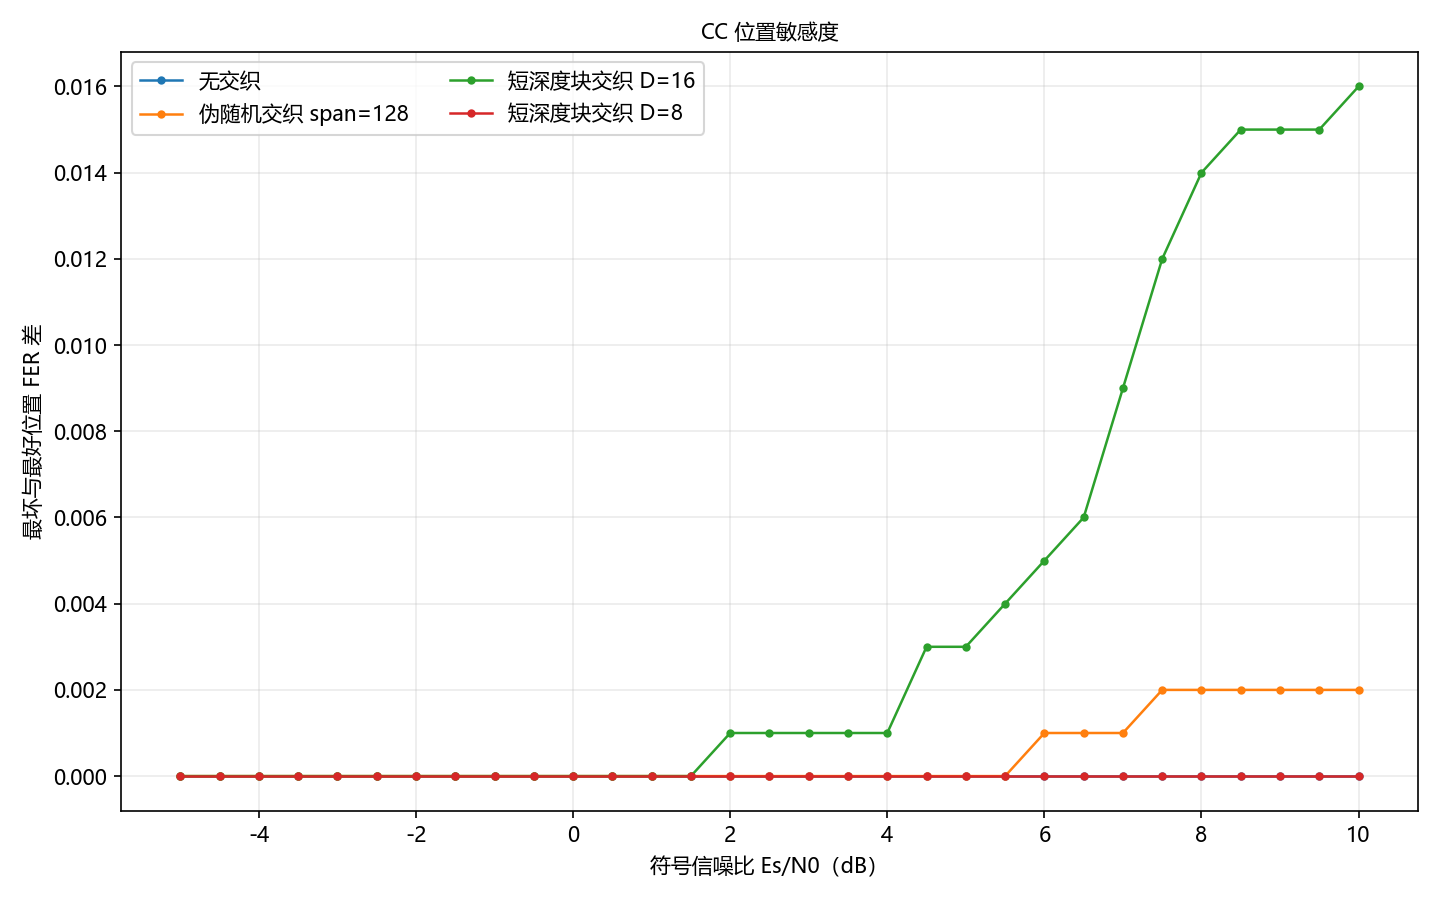
\includegraphics[width=\linewidth]{../Task/Comparison/S7/stage15_scientific_plots/results/cc/10_position_sensitivity/figure.png}\\[-0.2em]\small（b）位置敏感度
  \end{minipage}
  \caption{5\%突发条件下卷积码突发位置敏感性}
  \label{fig:s7-cc-position-detail}
\end{figure}

\subsection{短深度参数与等跨度受控比较}

卷积码的机理不同于BCH子块分散。连续异常集中在相邻trellis step时，会连续改变多个分支度量并影响局部路径竞争；交织把异常观测映射到更远的trellis位置，从而降低连续局部异常同时作用于相邻路径判决的程度。该映射不改变卷积码自由距离，也不改变编码器本身的理论纠错能力。

图\ref{fig:s7-cc-controlled}区分两类问题。左图比较同一规则块交织方法内部的$D=8$与$D=16$，反映深度与跨度变化；右图比较跨度均为128 trellis step、缓存均为256 bit的$D=16$与Pseudo128，反映相同资源边界下排列方式变化。$10$ dB、2\%条件下，$D=16$平均FER为0.718629，Pseudo128为0.448905，当前数据支持伪随机排列在该受控点具有更低FER。5\%条件下两者均接近饱和，差异不支持稳定的低FER排序。

\begin{figure}[htbp]
  \centering
  \begin{minipage}[t]{0.49\textwidth}
    \centering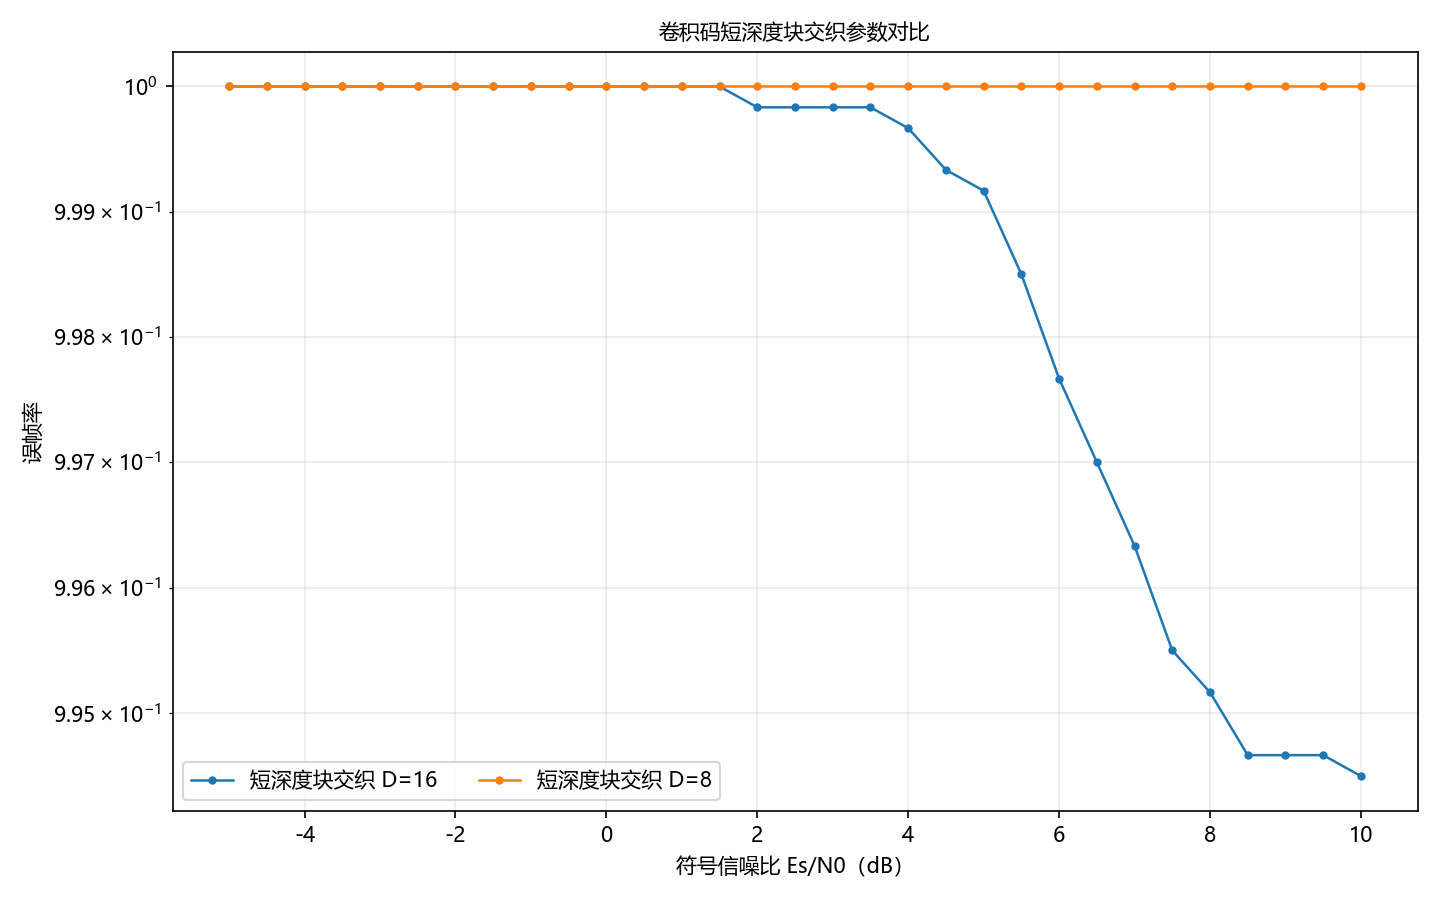
\includegraphics[width=\linewidth]{../Task/Comparison/S7/stage15_scientific_plots/results/cc/14_short_depth_parameters/figure.png}\\[-0.2em]\small（a）短深度参数比较
  \end{minipage}\hfill
  \begin{minipage}[t]{0.49\textwidth}
    \centering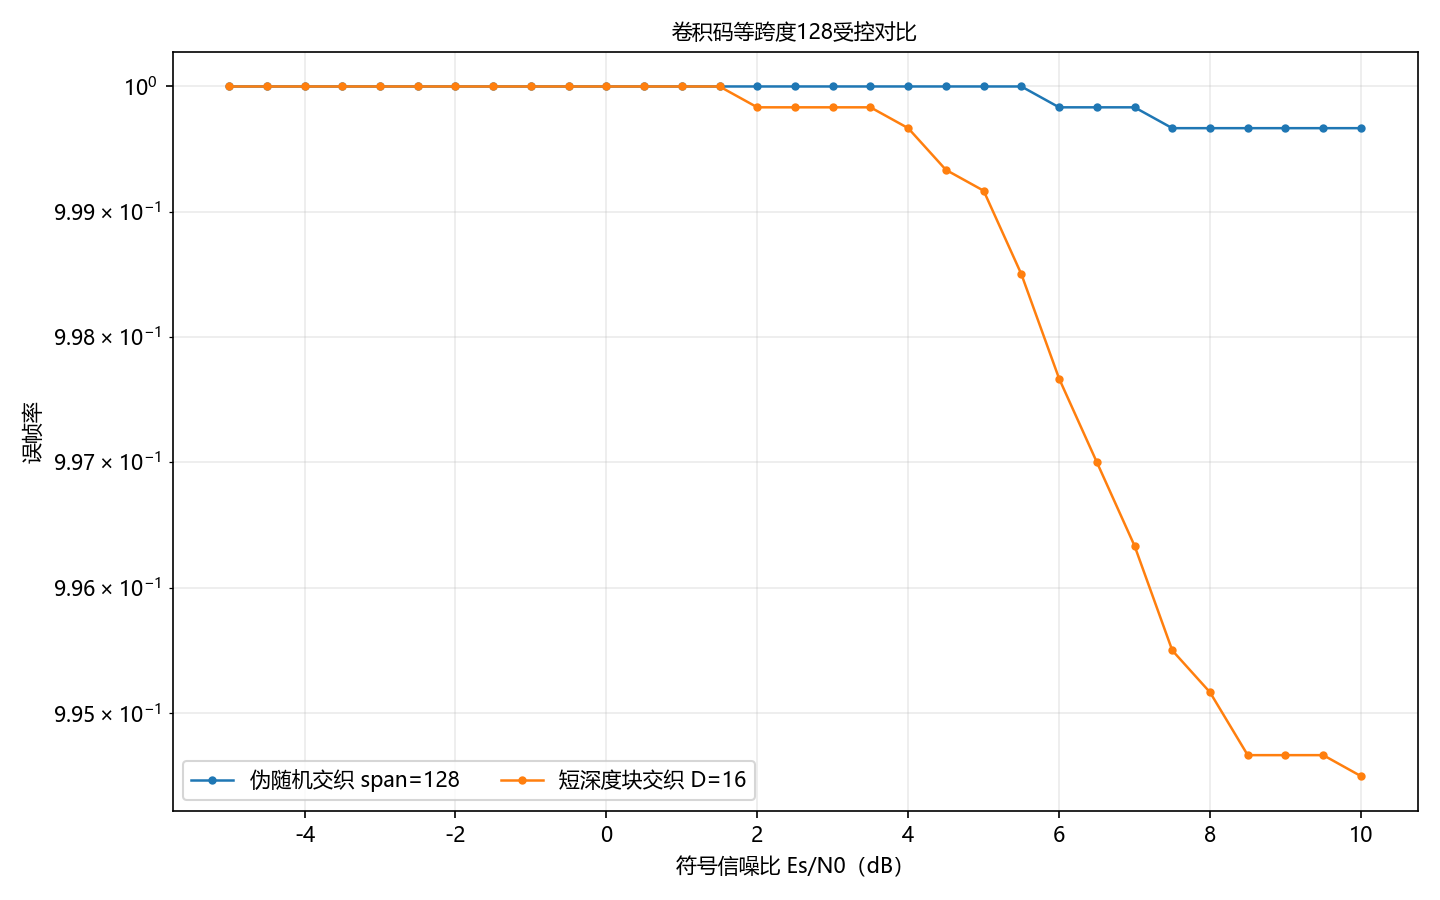
\includegraphics[width=\linewidth]{../Task/Comparison/S7/stage15_scientific_plots/results/cc/15_equal_span_128_controlled/figure.png}\\[-0.2em]\small（b）等跨度128受控比较
  \end{minipage}
  \caption{卷积码短深度与等跨度交织比较}
  \label{fig:s7-cc-controlled}
\end{figure}

\begin{table}[htbp]
  \centering
  \caption{卷积码短深度与等跨度受控比较（$E_s/N_0=10$ dB）}
  \label{tab:s7-cc-controlled}
  \footnotesize
  \begin{tabular}{clrrrp{0.26\textwidth}}
    \toprule
    突发 & 配置 & trellis跨度 & 缓存/bit & 平均FER & 比较角色 \\
    \midrule
    2\% & $D=8$ & 64 & 128 & 0.552654 & 低缓存工程配置 \\
    2\% & $D=16$ & 128 & 256 & 0.718629 & 等跨度规则排列 \\
    2\% & Pseudo128 & 128 & 256 & 0.448905 & 等跨度伪随机排列 \\
    5\% & $D=8$ & 64 & 128 & 1 & 低缓存工程配置 \\
    5\% & $D=16$ & 128 & 256 & 0.994500 & 等跨度规则排列 \\
    5\% & Pseudo128 & 128 & 256 & 0.999667 & 等跨度伪随机排列 \\
    \bottomrule
  \end{tabular}
\end{table}

图\ref{fig:s7-cc-fer-gain}给出5\%条件下的FER改善量。大部分工作点的改善接近零，且局部可能出现负改善，说明增大交织深度并不保证收益持续增加。当前数据中，Pseudo128在2\%高工作点具有较低平均FER；$D=8$以一半缓存获得可观测FER下降；$D=16$虽然增加到相同256 bit缓存，但并未形成一致优于$D=8$或Pseudo128的结果。性能随$D$增大并非单调改善，收益取决于突发长度、位置与排列结构。

\begin{figure}[htbp]
  \centering
  \begin{minipage}[t]{0.49\textwidth}
    \centering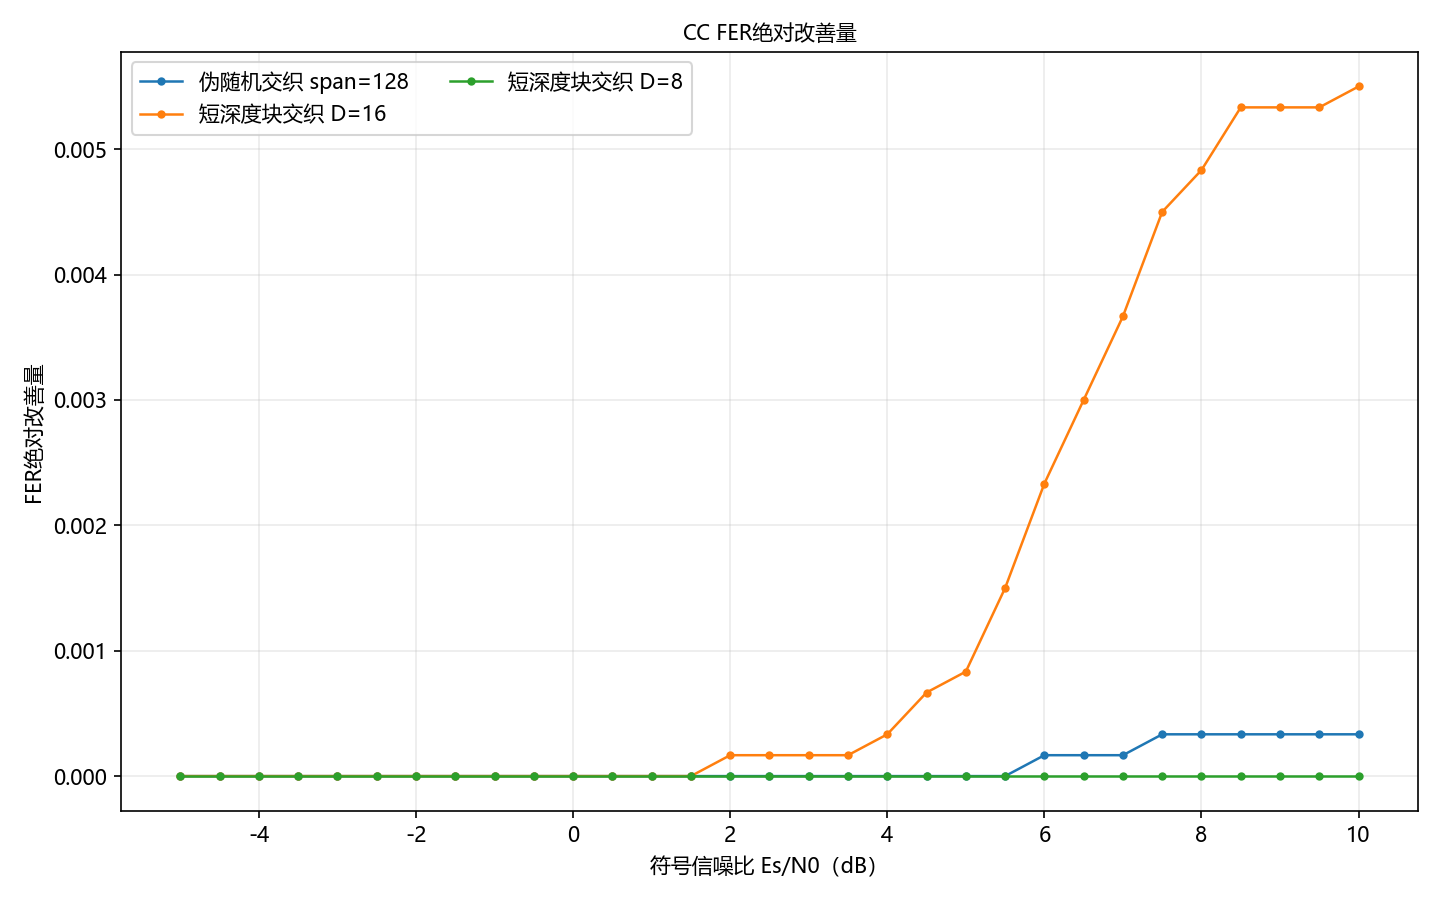
\includegraphics[width=\linewidth]{../Task/Comparison/S7/stage15_scientific_plots/results/cc/11_absoluteFerImprovement/figure.png}\\[-0.2em]\small（a）FER绝对改善量
  \end{minipage}\hfill
  \begin{minipage}[t]{0.49\textwidth}
    \centering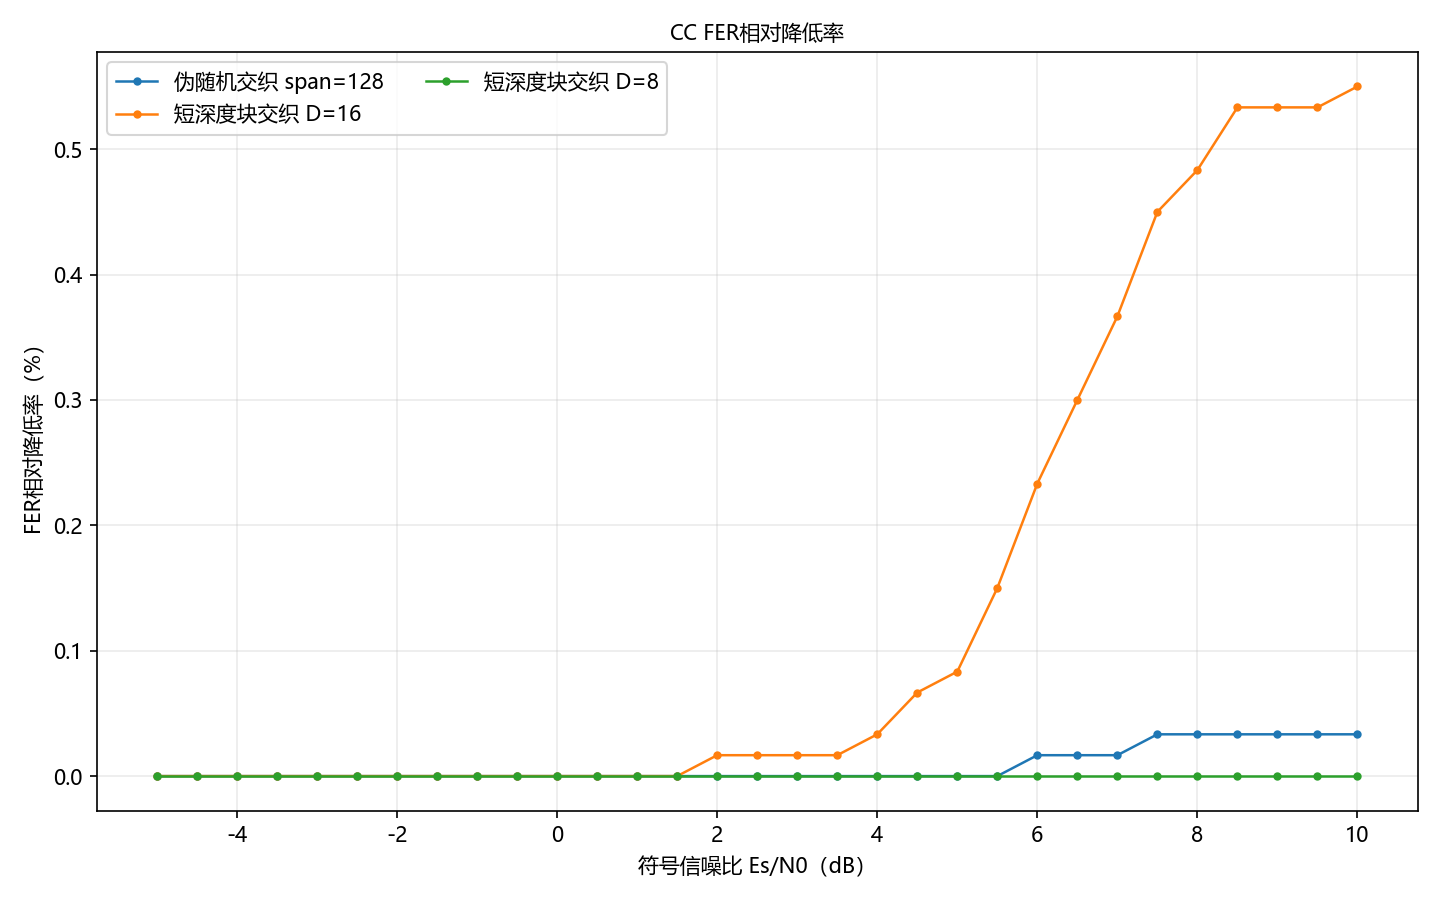
\includegraphics[width=\linewidth]{../Task/Comparison/S7/stage15_scientific_plots/results/cc/12_relativeFerReductionPercent/figure.png}\\[-0.2em]\small（b）FER相对降低率
  \end{minipage}
  \caption{5\%突发条件下卷积码交织的FER改善}
  \label{fig:s7-cc-fer-gain}
\end{figure}

\subsection{FER改善与突发错误容限}

卷积码高工作点容限结果显示，2\%条件下各交织配置的最坏位置FER均高于0.1，5\%条件下则均为1。因此，本章不把任何卷积码配置标记为通过该容限门限。与此同时，六位置平均FER仍能区分2\%条件下的配置差异：Pseudo128最低，$D=8$次之，$D=16$较高。平均性能与最坏位置门限回答的是不同问题，前者衡量总体配置收益，后者约束对突发起点敏感的业务风险。

在配置选择上，$D=8$以128 bit缓存取得44.73\%平均FER下降，Pseudo128以256 bit缓存取得55.11\%下降。增加128 bit缓存对应约10.38个百分点的平均FER相对降低差异，但最坏位置FER只从0.85变为0.84。若业务更重视平均帧成功率，可采用Pseudo128；若缓存受限且允许较高平均FER，$D=8$提供更紧凑的选择。该折中只适用于本章300 bit、终止整帧软Viterbi链路和已测试的2\%突发条件。

\subsection{缓冲需求与软件处理时间}

卷积码缓存量见图\ref{fig:s7-cc-buffer}。$D=8$需要暂存128个编码比特；$D=16$和Pseudo128均需要256个编码比特。按2\%和5\%正式仿真数据重新加权后，三种交织配置的交织CPU时间为737.4、742.7和751.8 ns/帧，去交织CPU时间为384.2、426.9和390.8 ns/帧，译码CPU时间约为$306.6\sim307.5~\mu$s/帧。与无交织配置相比，这些软件函数时间没有形成数量级增长；结构缓存则从0增加至128或256 bit。由于没有统一编码比特率或符号率，本章不把缓存量换算为微秒或毫秒。

\begin{figure}[htbp]
  \centering
  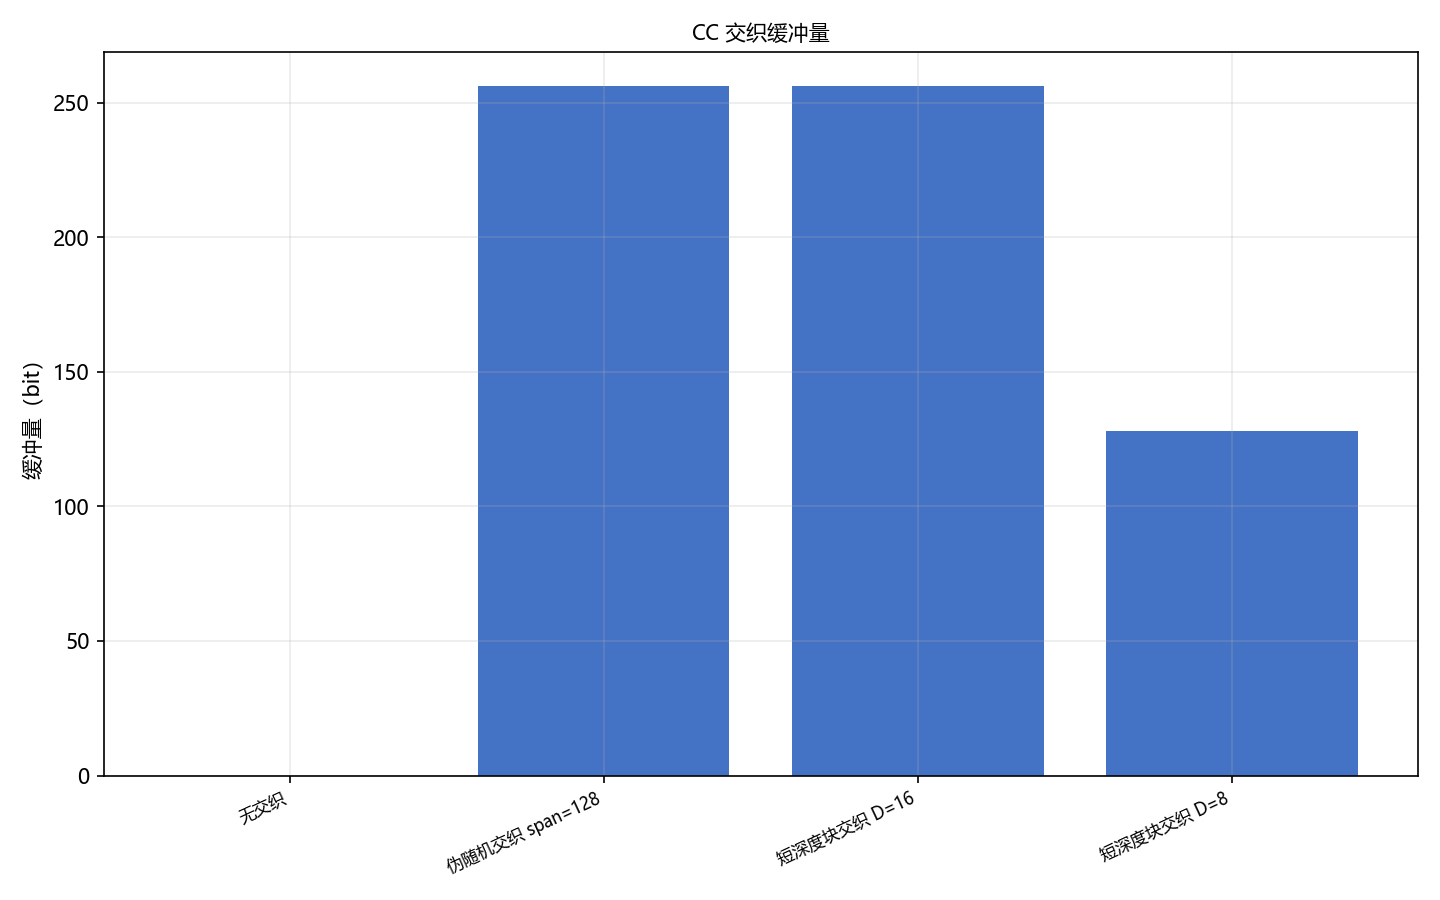
\includegraphics[width=0.88\textwidth]{../Task/Comparison/S7/stage15_scientific_plots/results/cc/19_bufferBits/figure.png}
  \caption{卷积码交织配置的结构缓存量}
  \label{fig:s7-cc-buffer}
\end{figure}

\section{LDPC无交织近码率基线}

本节只比较无突发AWGN条件下的卷积码与LDPC N640基线。两者有效载荷均为300 bit，实际码率分别为0.490196和0.468750，相对码率差约4.375\%。LDPC采用BG2、$Z=40$、layered NMS译码，归一化系数0.80，最多32次迭代；两种方案均不使用交织。表\ref{tab:s7-cc-ldpc-baseline}中的BER和FER取$E_s/N_0=0.5$ dB正式点，软件译码时间为各自正式AWGN点的帧数加权参考。

\begin{table}[htbp]
  \centering
  \caption{卷积码与LDPC无交织近码率基线}
  \label{tab:s7-cc-ldpc-baseline}
  \footnotesize
  \resizebox{\textwidth}{!}{%
  \begin{tabular}{lrrrrrlp{4.2cm}}
    \toprule
    方案 & 载荷/bit & 发送/bit & 码率 & FER & BER & 译码CPU/ns每帧 & 角色 \\
    \midrule
    卷积码 & 300 & 612 & 0.490196 & 0.0048944 & $7.29\times10^{-5}$ & 428650 & 无交织、无突发AWGN参考 \\
    LDPC N640 & 300 & 640 & 0.468750 & $6.0\times10^{-5}$ & $1.0\times10^{-6}$ & 93743 & 无交织、无突发AWGN近码率参考 \\
    \bottomrule
  \end{tabular}}
\end{table}

图\ref{fig:s7-cc-ldpc-latency}给出相同加权口径的软件译码CPU时间参考。卷积码可描述306个trellis step、64状态及分支度量与加比选过程；LDPC可描述N640、边消息更新和平均迭代，但两类操作不能直接相加为统一操作数，也不能把该软件时间直接解释为硬件实现时延。

\begin{figure}[htbp]
  \centering
  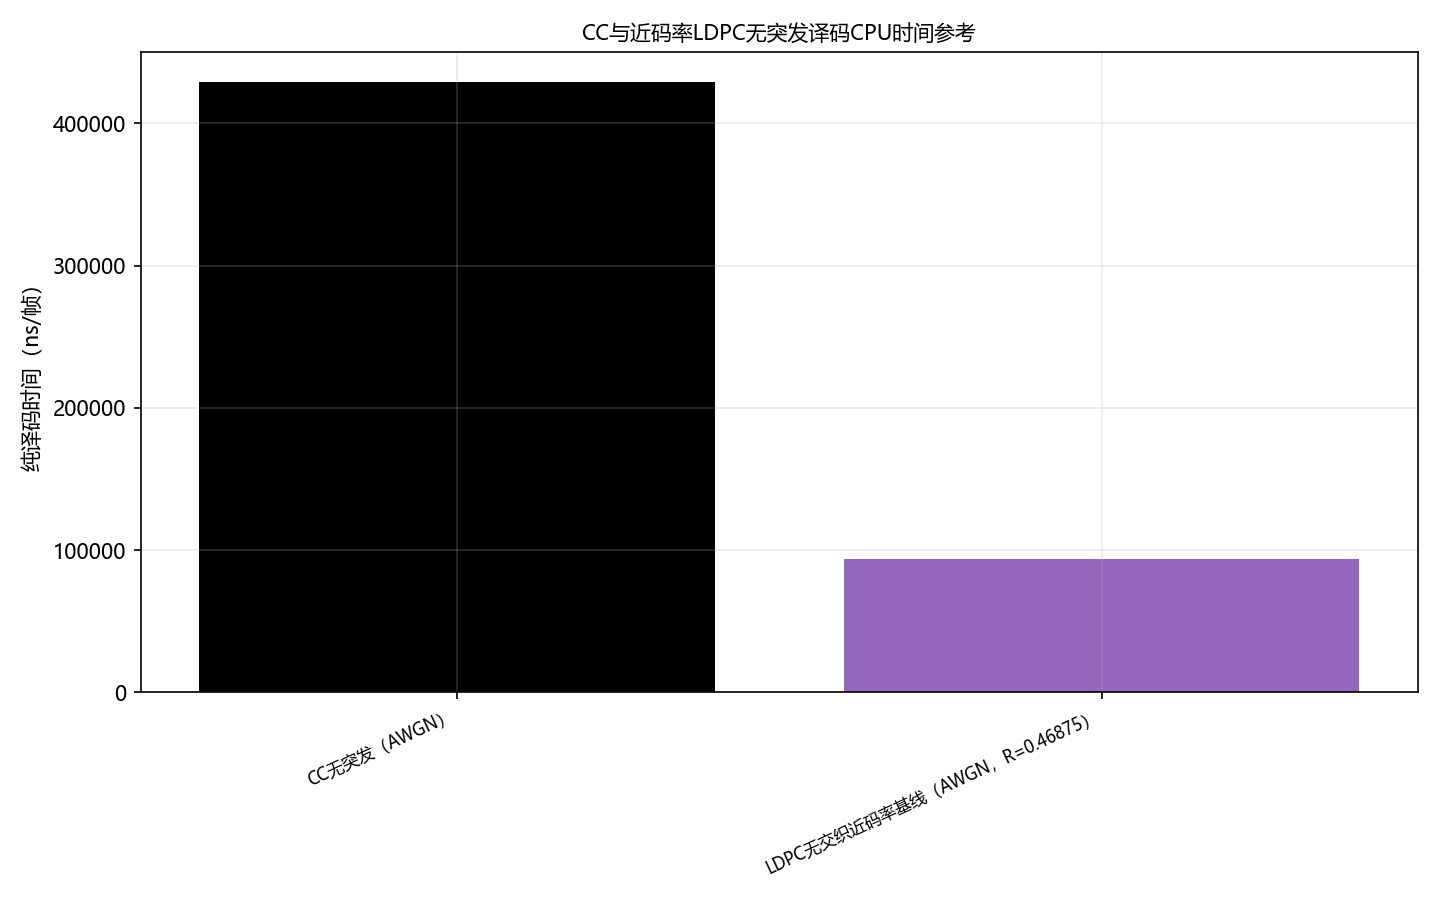
\includegraphics[width=0.88\textwidth]{../Task/Comparison/S7/stage15_scientific_plots/results/cc/22_cc_ldpc_no_burst_decode_latency/figure.png}
  \caption{卷积码与LDPC无交织、无突发AWGN软件译码CPU时间参考}
  \label{fig:s7-cc-ldpc-latency}
\end{figure}

该基线能够说明：在接近码率和相同有效载荷下，当前LDPC实现的AWGN误码、误帧结果及软件译码时间可作为高速编码方案参照。它不能说明LDPC在2\%或5\%突发条件下的性能，也不能给出LDPC的交织收益、突发容限或位置敏感性。LDPC不进入本章交织配置排名。

\section{交织收益与工程代价综合分析}

表\ref{tab:s7-buffer-time}统一列出仅按2\%和5\%正式仿真数据加权的软件时间。BCH三种交织方法均缓存285 bit，交织与去交织函数合计约$0.65~\mu$s/帧；卷积码$D=8$缓存128 bit，Pseudo128和$D=16$缓存256 bit，交织与去交织函数合计约$1.12\sim1.17~\mu$s/帧。软件CPU时间不等价于物理链路等待，缓存bit数也不等价于时延数值。工程实现仍需结合实际编码比特率、存储结构和硬件并行度换算。

\begin{table}[htbp]
  \centering
  \caption{交织缓存与软件CPU处理时间（仅2\%和5\%行加权）}
  \label{tab:s7-buffer-time}
  \footnotesize
  \begin{tabular}{llrrrr}
    \toprule
    方案 & 配置 & 缓存/bit & 交织/ns & 去交织/ns & 译码/ns \\
    \midrule
    BCH & 无交织 & 0 & 328.4 & 310.5 & 8424 \\
    BCH & 子块结构$D=19$ & 285 & 324.9 & 329.9 & 8998 \\
    BCH & 行列$R=15$ & 285 & 325.3 & 322.6 & 8886 \\
    BCH & 全帧伪随机 & 285 & 325.1 & 324.6 & 8755 \\
    卷积码 & 无交织 & 0 & 745.8 & 404.4 & 307767 \\
    卷积码 & 短深度$D=8$ & 128 & 737.4 & 384.2 & 307483 \\
    卷积码 & Pseudo128 & 256 & 751.8 & 390.8 & 307488 \\
    卷积码 & 短深度$D=16$ & 256 & 742.7 & 426.9 & 306640 \\
    \bottomrule
  \end{tabular}
\end{table}

高工作点最坏位置FER见表\ref{tab:s7-burst-tolerance}。在当前测试网格与FER不高于0.1的判据下，BCH子块结构和行列交织均通过2\%与5\%条件；无交织和全帧伪随机配置未通过。卷积码四种配置在2\%和5\%的最坏位置均未通过该门限。该表只描述已测试的两档条件，不在网格之间插值，也不把LDPC加入突发错误容限判断。

\begin{table}[htbp]
  \centering
  \caption{高工作点突发错误容限（最坏位置FER）}
  \label{tab:s7-burst-tolerance}
  \footnotesize
  \begin{tabular}{llrrrr}
    \toprule
    方案 & 配置 & 2\%长度/bit & 2\%最坏FER & 5\%长度/bit & 5\%最坏FER \\
    \midrule
    BCH & 无交织 & 6 & 1 & 14 & 1 \\
    BCH & 子块结构$D=19$ & 6 & $4.40\times10^{-4}$ & 14 & 0.00102 \\
    BCH & 行列$R=15$ & 6 & $5.00\times10^{-4}$ & 14 & $8.80\times10^{-4}$ \\
    BCH & 全帧伪随机 & 6 & 0.99998 & 14 & 1 \\
    卷积码 & 无交织 & 12 & 1 & 31 & 1 \\
    卷积码 & 短深度$D=8$ & 12 & 0.85 & 31 & 1 \\
    卷积码 & Pseudo128 & 12 & 0.84 & 31 & 1 \\
    卷积码 & 短深度$D=16$ & 12 & 1 & 31 & 1 \\
    \bottomrule
  \end{tabular}
\end{table}

综合建议见表\ref{tab:s7-engineering-recommendation}。对本章200 bit分块BCH方案，行列$R=15$在两档突发高工作点均取得最低六位置平均FER，可作为性能优先配置；子块结构$D=19$的结果接近，并具有与19个BCH子块直接对应的结构解释。两者缓存相同，软件处理时间差异很小。全帧伪随机置换虽覆盖相同跨度，但位置稳定性和平均FER均不足以替代两种规则结构方案。

对300 bit卷积码，配置选择需要区分性能与缓存目标。Pseudo128在2\%高工作点获得最低平均FER，但需要256 bit缓存；$D=8$以128 bit缓存获得44.73\%的平均FER下降，可作为缓存优先配置。$D=16$增加到256 bit缓存后未形成稳定增益，说明单纯增加深度的收益趋于不稳定。5\%条件下各配置FER接近饱和，因此当前证据不支持将任何卷积码交织配置描述为31 bit突发下的低FER方案。

\begin{table}[htbp]
  \centering
  \caption{S7工程配置建议}
  \label{tab:s7-engineering-recommendation}
  \small
  \begin{tabular}{p{0.13\textwidth}p{0.25\textwidth}p{0.18\textwidth}p{0.34\textwidth}}
    \toprule
    方案 & 建议配置 & 适用目标 & 证据边界 \\
    \midrule
    分块BCH & 行列$R=15$ & 性能优先 & 两档高工作点平均FER最低；仅限本章200 bit分块方案 \\
    分块BCH & 子块结构$D=19$ & 结构清晰备选 & 性能接近行列方案；不改变单块理论纠错能力 \\
    卷积码 & 短深度$D=8$ & 缓存优先 & 128 bit缓存；与Pseudo128不是等跨度纯方法比较 \\
    卷积码 & Pseudo128 & 2\%条件FER优先 & 256 bit缓存；5\%条件下未形成低FER工作点 \\
    \bottomrule
  \end{tabular}
\end{table}

\section{本章结论}
\enlargethispage{5\baselineskip}

本章在固定编码与译码方案下比较了2\%和5\%连续突发错误。对200 bit分块BCH方案，无交织时错误集中在较少的15 bit子块，单块多错误事件频繁；子块结构交织和行列交织把异常分散到约14个子块，并在$10$ dB、5\%条件下把单块最大错误数从15降至2，使更多子块落入BCH(15,11,1)原有单比特可纠正范围。两种规则结构交织的平均FER均由无交织的1降至$10^{-3}$以下，其中行列$R=15$为$7.63\times10^{-4}$。该结论限定于本章采用的分块BCH方案。

对300 bit卷积码，连续异常集中作用于相邻trellis step并改变局部路径度量竞争；交织将异常观测映射到更远的trellis位置。2\%条件下，$10$ dB处$D=8$和Pseudo128的平均FER分别为0.552654和0.448905，均低于无交织的1；5\%条件下所有配置仍接近FER饱和。$D=8$与Pseudo128是不同跨度和缓存规模的工程配置，$D=16$与Pseudo128才构成128 trellis step等跨度受控比较。增大$D$没有形成单调收益，交织也没有改变卷积码自由距离。

工程代价方面，BCH规则结构交织需要285 bit缓存，卷积码$D=8$与Pseudo128分别需要128 bit和256 bit缓存。仅按正式展示条件加权的软件交织与去交织时间均远小于对应译码函数时间，但这些CPU测量不能替代物理链路时延。LDPC N640只提供无交织、无突发AWGN近码率参考，能够支持高速编码方案的AWGN性能与软件实现对照，不能支持突发错误性能、交织排名或位置敏感性结论。

\chapter{综合方案推荐与结论}\label{chap:recommendation}

\section{综合选型原则}

信道编码方案应首先按业务类型分流。200 bit与300 bit低速电文采用BCH候选，300 bit高速电文采用卷积码或LDPC候选；三类编码承载的业务、发送长度和处理机制不同，不建立跨业务统一排名。在业务边界确定后，系统依次检查目标FER覆盖、实际发送长度与码率、实时处理和实现资源、信道适应性，最后决定是否配置交织。该顺序延续表\ref{tab:bch-conclusions}、表\ref{tab:cc-main-conclusions}、表\ref{tab:cc-system-recommendations}、表\ref{tab:ldpc-length-tradeoff}和表\ref{tab:ldpc-decoder-tradeoff}已经冻结的码族内部结论。

可靠性是进入后续比较的前置条件。方案若在规定信噪比范围内不能覆盖目标FER，或在目标场景中形成明显错误平台，则不能仅凭较高码率或较短软件CPU时间成为主推荐。可靠性满足后，再比较payload之外的tail、filler、shortening和puncturing所形成的实际发送长度。实时性评价同时考虑首次输出、P95、最大观测软件时间、迭代上限、回溯深度和结构缓存；其中CPU时间只描述当前处理器、编译器和计时边界，不能直接等同于硬件时延。

信道适应性依据第7章的AWGN、固定多径、固定频偏、线性时变频偏、已知短时遮挡和未知突发结果，近码率横向选择以表\ref{tab:s5-recommendations}为最高优先级证据。交织不是常驻模块，只在连续错误集中出现且已有正式试验支持时启用。表\ref{tab:s7-engineering-recommendation}所支持的BCH与卷积码配置均受第9章具体码型和突发比例约束，LDPC则保持无交织。

\begin{table}[htbp]
  \centering\scriptsize
  \caption{综合选型判据与证据来源}
  \label{tab:final-selection-criteria}
  \resizebox{\textwidth}{!}{\begin{tabular}{c l l l l}
    \toprule
    决策层级 & 工程问题 & 核心指标 & 主要证据章节 & 使用边界 \\
    \midrule
    业务 & 低速或高速、payload长度 & 200/300 bit、业务接口 & 第2、4--7章 & 禁止跨业务统一排名 \\
    可靠性 & 是否覆盖目标工作点 & FER、BER、错误平台 & 表\ref{tab:bch-conclusions}、\ref{tab:s5-recommendations} & 未覆盖目标者不进入效率优选 \\
    传输效率 & 每帧实际占用多少符号 & 发送长度、实际码率、填充与打孔 & 表\ref{tab:cc-main-conclusions}、\ref{tab:ldpc-length-tradeoff} & 固定$E_s/N_0$与固定$E_b/N_0$不可混用 \\
    实时性 & 何时产生稳定输出 & 首输出、P95、最大观测、迭代与回溯 & 表\ref{tab:cc-system-recommendations}、\ref{tab:s6-engineering-summary} & 软件CPU时间不等于物理链路时延 \\
    实现资源 & 译码与缓存是否可承受 & 状态数、图规模、存储、buffer & 表\ref{tab:s6-engineering-summary} & 不统一折算异构操作次数 \\
    信道适应性 & 非理想信道下是否保持覆盖 & 六类信道FER门限与损失 & 表\ref{tab:s5-recommendations} & 仅适用于第7章规定模型 \\
    突发与交织 & 是否需要重排错误位置 & 平均/最坏FER、跨度、缓存 & 表\ref{tab:s7-engineering-recommendation} & 仅外推到已验证码型与突发比例 \\
    \bottomrule
  \end{tabular}}
\end{table}

\section{低速电文BCH综合推荐}

200 bit业务形成低复杂度、高可靠性和明显连续突发三条路线。资源受限且信道以分散错误为主时，主推荐$19\times\mathrm{BCH}(15,11,1)$：200 bit payload补9 bit后形成19个11 bit子块，发送285 bit，实际码率为$200/285\approx0.701754$，采用综合校验查表译码。该路线结构短、查表路径直接，在当前软件实现中译码时间较低；代价是AWGN可靠性低于较长整块BCH。

常规信道可靠性优先时，主推荐缩短$\mathrm{BCH}(511,385)$，发送326 bit、$t=14$，实际码率为$200/326\approx0.613497$，采用BM与Chien搜索。该配置以更多发送冗余和较高代数译码开销换取第4章正式AWGN结果中的较高可靠性。对明显连续突发，结论只适用于上述200 bit分块方案：性能优先采用行列交织R15，结构组织优先可采用D19；两者均缓存完整285 coded bits。第9章并未验证200 bit整块BCH或300 bit整块BCH的同类交织，因此不得据此扩展。

300 bit业务不新增交织路线。综合平衡主推荐缩短$\mathrm{BCH}(511,421)$，发送390 bit、$t=10$，实际码率$300/390\approx0.769231$；可靠性优先采用缩短$\mathrm{BCH}(511,385)$，发送426 bit、$t=14$，实际码率$300/426\approx0.704225$。两者均采用BM与Chien搜索，选择实质是90 bit与126 bit冗余之间的可靠性和发送占用取舍。

\begin{table}[htbp]
  \centering\scriptsize
  \caption{低速BCH最终推荐矩阵}
  \label{tab:final-bch-matrix}
  \resizebox{\textwidth}{!}{\begin{tabular}{c l l l c c l l}
    \toprule
    信息长度 & 目标/场景 & 主推荐 & 译码器/交织 & 发送长度 & 实际码率 & 主要依据 & 主要代价或边界 \\
    \midrule
    200 & 低复杂度 & $19\times\mathrm{BCH}(15,11,1)$ & 查表/NONE & 285 & 0.701754 & 短码与最低软件译码时间 & AWGN可靠性低于长整块方案 \\
    200 & 常规可靠性 & 缩短$\mathrm{BCH}(511,385)$，$t=14$ & BM+Chien/NONE & 326 & 0.613497 & 第4章AWGN可靠性优先 & 冗余与代数译码开销较高 \\
    200 & 明显连续突发 & 分块BCH & 查表/R15，D19备选 & 285 & 0.701754 & 表\ref{tab:s7-engineering-recommendation} & 仅限200 bit分块方案，缓存285 bit \\
    300 & 综合平衡 & 缩短$\mathrm{BCH}(511,421)$，$t=10$ & BM+Chien/NONE & 390 & 0.769231 & 表\ref{tab:bch-conclusions} & 不含正式交织验证 \\
    300 & 可靠性优先 & 缩短$\mathrm{BCH}(511,385)$，$t=14$ & BM+Chien/NONE & 426 & 0.704225 & 更强纠错能力 & 发送占用与译码开销增加 \\
    \bottomrule
  \end{tabular}}
\end{table}

\section{高速电文卷积码综合推荐}

高速卷积码统一采用300 bit payload、约束长度$K=7$、八进制生成多项式171/133、6 bit零尾和64个状态。软判决Viterbi为性能主路线，硬判决仅作为接收接口或资源极紧条件下的备选。表\ref{tab:cc-main-conclusions}显示，在FER$=0.1$处，浮点软判决相对硬判决的$E_s/N_0$收益为1.857--2.085 dB；这一收益来自更完整的幅度可靠性，而不增加发送冗余。

五类系统配置服务于不同基准，不构成统一排名。可靠性优先采用$1/2$母码、612 bit发送和整块浮点软判决；吞吐优先采用约$3/4$打孔、408 bit发送及$W=160,S=25,D=126$；时延优先采用约$2/3$打孔、459 bit发送及$W=128,S=25,D=84$；存储优先和综合平衡均采用$1/2$母码与$W=96,S=16,D=70$。高码率配置只有在链路FER余量满足时才具有工程意义。

连续时隙需要分批交付时，优先采用$50\times6$组织。$50\times6$、$100\times3$和$150\times2$产生相同最终码流，FER与BER不因组织方式改变；选择$50\times6$依据的是等待分布和P95输出时间，而不是更高可靠性。定点软信息实现优先采用Q8，第5章在FER$=0.1$处给出的相对浮点损失处于约0.008 dB以内量级，但系统性能基准仍以浮点软判决为准。

\begin{table}[htbp]
  \centering\scriptsize
  \caption{卷积码系统级最终配置矩阵}
  \label{tab:final-cc-matrix}
  \resizebox{\textwidth}{!}{\begin{tabular}{l c c l c c c l l}
    \toprule
    工程目标 & 实际码率 & 发送长度 & 译码方式 & $W$ & $S$ & $D$ & 时隙/软信息 & 选择理由与边界 \\
    \midrule
    可靠性优先 & 0.4902 & 612 & 整块浮点软Viterbi & -- & -- & 306 & 整帧/浮点 & 冗余充分；等待完整码字 \\
    吞吐优先 & 0.7353 & 408 & 滑窗软Viterbi & 160 & 25 & 126 & 连续/浮点 & 发送最短；仅在FER余量允许时使用 \\
    时延优先 & 0.6536 & 459 & 滑窗软Viterbi & 128 & 25 & 84 & $50\times6$/浮点 & 较早分批输出；可靠性低于$1/2$母码 \\
    存储优先 & 0.4902 & 612 & 滑窗软Viterbi & 96 & 16 & 70 & 连续/浮点 & 覆盖既定FER门限且译码存储较低 \\
    综合平衡 & 0.4902 & 612 & 滑窗软Viterbi & 96 & 16 & 70 & $50\times6$/Q8优先 & Q8为实现配置，浮点仍是性能基准 \\
    \bottomrule
  \end{tabular}}
\end{table}

\section{高速电文LDPC综合推荐}

三种BG2 Direct QC-LDPC短块配置均承载300 bit payload，最大迭代次数为32。N480发送480 bit、实际码率0.6250，适用于传输效率优先；N560发送560 bit、实际码率0.5357，其价值是接近576 bit目标的接口适配，不作为默认综合最优；N640发送640 bit、实际码率0.46875，适用于可靠性和弱信号优先。归一化系数必须随码长配置：N480和N560取$\alpha=0.95$，N640取$\alpha=0.80$。

工程译码优先采用layered NMS，BP保留为性能参考。在第8章统一的N560对比中，NMS相对BP的目标FER性能损失小于约0.04 dB，同时当前软件处理时间显著下降；更广的第6章结果亦表明两者目标FER门限接近。该结论只说明当前算法、数据结构和软件环境下NMS具有更合适的实现取舍，不表示其在所有平台或所有迭代调度下全面优于BP。

\begin{table}[htbp]
  \centering\scriptsize
  \caption{LDPC最终推荐配置}
  \label{tab:final-ldpc-matrix}
  \resizebox{\textwidth}{!}{\begin{tabular}{l c c l c c l l}
    \toprule
    目标 & 码长 & 实际码率 & 译码器 & $\alpha$ & 最大迭代 & 主要优势 & 主要代价与定位 \\
    \midrule
    传输效率 & 480 & 0.6250 & layered NMS & 0.95 & 32 & LDPC候选中发送最短 & 可靠性低于N640 \\
    接口适配 & 560 & 0.5357 & layered NMS & 0.95 & 32 & 接近576 bit接口目标 & 非默认性能折中 \\
    可靠性/弱信号 & 640 & 0.46875 & layered NMS & 0.80 & 32 & 更完整的低FER覆盖 & 发送与校验图规模较大 \\
    性能参考 & 480/560/640 & 对应码率 & layered BP & -- & 32 & 和积算法基准 & 当前软件时间明显高于NMS \\
    \bottomrule
  \end{tabular}}
\end{table}

\section{高速电文卷积码与LDPC场景化选择}

近$2/3$组比较CC R2/3（实际码率约0.6536）与LDPC N480（0.6250），属于近码率而非完全同码率比较。表\ref{tab:s5-recommendations}表明，在AWGN、固定多径、固定频偏和线性时变频偏下，CC R2/3的绝对FER门限均更低，因而成为常规全帧信道主推荐；在已知5\%短时遮挡下，N480保持FER$=0.1$目标覆盖，而CC未形成相同覆盖，N480转为该场景的主候选。未知5\%突发干扰下，两者均未形成稳定低FER结果，当前无已验证的稳定低FER主方案。

近$1/2$组比较CC R1/2（约0.4902）与LDPC N640（0.46875）。N640在AWGN、固定多径、固定频偏和线性时变频偏下具有更低绝对FER门限，并在已知5\%遮挡下形成更完整的目标覆盖，可靠性和弱信号优先时应采用N640。CC R1/2仍具有固定64状态、无需迭代、可滑窗和可分批输出等实时实现优势，适用于连续处理或可预测等待优先的系统。未知5\%突发下，N640只表现出有限FER$=0.1$覆盖且明显退化，CC未形成相同低FER覆盖，因此不把任一方案写成稳定主推荐。

\begin{table}[htbp]
  \centering\scriptsize
  \caption{高速电文场景化方案选择矩阵}
  \label{tab:final-highspeed-scenarios}
  \resizebox{\textwidth}{!}{\begin{tabular}{c l l l l l}
    \toprule
    目标码率组 & 信道场景 & 主推荐 & 备选 & 可靠性与实现依据 & 边界 \\
    \midrule
    近$2/3$ & AWGN/固定多径 & CC R2/3软Viterbi & N480 NMS & CC绝对FER门限更低，固定64状态 & 近码率比较 \\
    近$2/3$ & 固定/时变频偏 & CC R2/3软Viterbi & N480 NMS & CC绝对FER门限更低 & 依赖规定帧内相位轨迹 \\
    近$2/3$ & 已知5\%遮挡 & N480 NMS & -- & N480保持FER$=0.1$覆盖 & 受损位置已知 \\
    近$2/3$ & 未知5\%突发 & 无已验证稳定低FER主方案 & -- & 两者均未形成稳定低FER结果 & 不能强行外推 \\
    \midrule
    近$1/2$ & AWGN/固定多径 & N640 NMS & CC R1/2软Viterbi & N640绝对FER门限更低 & CC适合实时连续处理 \\
    近$1/2$ & 固定/时变频偏 & N640 NMS & CC R1/2软Viterbi & N640绝对FER门限更低 & 依赖规定帧内相位轨迹 \\
    近$1/2$ & 已知5\%遮挡 & N640 NMS & -- & N640目标覆盖更完整 & 受损位置已知 \\
    近$1/2$ & 未知5\%突发 & 无已验证稳定低FER主方案 & N640性能参考 & N640仅有限FER$=0.1$覆盖 & 两者均明显退化 \\
    \bottomrule
  \end{tabular}}
\end{table}

\section{译码、连续处理与交织联合配置}

译码器与交织器必须同具体码型和业务条件联合选择。低复杂度200 bit分块BCH在分散错误下使用查表且不交织，明显连续突发时配置R15，D19作为结构清晰的备选；整块BCH采用BM与Chien搜索且不交织。卷积码常规链路采用软Viterbi并关闭交织，需要连续输出时按目标选取表\ref{tab:final-cc-matrix}中的滑窗和时隙参数。

卷积码在2\%突发下可按资源切换：缓存优先采用D8，跨度64 trellis steps、缓存128 coded bits；FER优先采用Pseudo128，跨度128 trellis steps、缓存256 coded bits。D8与Pseudo128是不同资源规模的工程配置比较；只有D16与Pseudo128构成相同128 trellis-step跨度和256 coded-bit缓存下的受控排列比较。5\%突发下全部正式卷积码交织配置仍接近FER饱和，当前未形成满足低FER要求的稳定配置。LDPC始终采用NONE interleaver与NMS；第9章LDPC数据只承担无突发AWGN近码率基线，不能据此推断其突发性能。

\begin{table}[htbp]
  \centering\scriptsize
  \caption{译码与交织联合配置}
  \label{tab:final-decoder-interleaver}
  \resizebox{\textwidth}{!}{\begin{tabular}{l l l l c l l}
    \toprule
    编码方案 & 常规译码 & 连续处理 & 突发配置 & 结构缓存/bit & 适用条件 & 禁止外推范围 \\
    \midrule
    200 bit分块BCH & 查表 & 整帧 & R15主、D19备选 & 285 & 明显2\%/5\%连续突发 & 不扩展到整块或300 bit BCH \\
    整块BCH & BM+Chien & 整帧 & NONE & 0 & 常规分散错误 & 无正式交织结论 \\
    CC常规 & 浮点软Viterbi，硬判决备选 & 滑窗/$50\times6$ & NONE & 0 & 常规信道与连续输出 & 参数按具体码率选择 \\
    CC 2\%突发 & 软Viterbi & 整帧 & D8/缓存优先 & 128 & 64 trellis-step跨度 & 与Pseudo128非等资源比较 \\
    CC 2\%突发 & 软Viterbi & 整帧 & Pseudo128/FER优先 & 256 & 128 trellis-step跨度 & 5\%下无稳定低FER恢复 \\
    LDPC & layered NMS，BP参考 & 码块迭代 & NONE & 0 & 已验证无突发及第7章信道 & 第9章不支持突发性能推断 \\
    \bottomrule
  \end{tabular}}
\end{table}

\section{最终推荐方案}

最终配置遵循“主推荐、备选、条件切换”三级表达。低速业务先按payload和复杂度、可靠性或突发目标选择BCH；高速业务先按目标码率组与信道场景选择CC或LDPC，再叠加译码、连续组织与交织配置。高速吞吐优先可采用CC约$3/4$与$W=160,S=25,D=126$，但必须先验证业务工作点保有足够FER余量。未知强突发没有为了填满配置表而指定未经验证的赢家。

工程控制面应把payload长度、目标FER、目标码率组、信道状态类别、实时预算和突发状态作为显式输入，不以单一“最佳编码”标志代替完整配置。一次模式选择至少同时下发编码方案标识、发送长度、译码器类型、软信息格式、滑窗参数、交织模式和缓存需求；接收端只有在这些字段与发送端一致时才启动对应译码流程。BCH的分组/整块切换会改变码字组织与译码器，卷积码的打孔切换会改变去打孔图样和发送长度，LDPC码长切换会改变提升因子、校验图与$\alpha$，因此均不能只修改名义码率而沿用旧状态。

条件切换也应设置滞回和最小保持时间，避免信道估计在门限附近波动时频繁改变码型。若可靠性监测显示主方案不再覆盖目标，应先降码率或切换至对应可靠性候选；若链路余量恢复且发送占用成为主要约束，再转回效率候选。突发告警只有在受损模式与第9章验证边界一致时才启用交织；未知强突发则进入降级状态，不以未经验证的交织配置维持正常业务声明。

每次配置迁移需重新执行无噪声编译码一致性、实际发送长度、FER工作点、输出时序和缓存上限五项验收。对卷积码还应验证尾比特和连续状态边界，对LDPC验证综合校验与最大迭代退出，对交织链路验证交织/解交织互逆。该验收集合使表\ref{tab:final-recommendations}成为可执行配置入口，同时保留前文各项Formal结果的适用条件。

\begin{figure}[htbp]
  \centering
  \fbox{\begin{minipage}[c][0.22\textheight][c]{0.88\textwidth}
    \centering
    \textbf{待插入：Visio综合选型流程图}\\[0.6em]
    电文业务 $\rightarrow$ 低速BCH / 高速目标码率\\
    低速：200/300 bit $\rightarrow$ 复杂度、可靠性或突发目标\\
    高速：近$2/3$ / 近$1/2$ $\rightarrow$ 信道、实时性与吞吐目标\\
    输出：编码、译码、连续组织、交织及条件切换
  \end{minipage}}
  \caption{低速与高速电文信道编码综合选型流程}
  \label{fig:final-selection-visio}
\end{figure}

\begin{table}[htbp]
  \centering\tiny
  \caption{最终方案总表}
  \label{tab:final-recommendations}
  \resizebox{\textwidth}{!}{\begin{tabular}{c c l l l l l l l}
    \toprule
    业务 & payload & 主要目标/场景 & 主推荐编码 & 码率/长度 & 译码与连续组织 & 交织 & 备选 & 适用边界 \\
    \midrule
    低速 & 200 & 低复杂度 & $19\times$BCH(15,11,1) & 0.701754/285 & 查表/整帧 & NONE & -- & 分散错误 \\
    低速 & 200 & 常规可靠性 & BCH(511,385) & 0.613497/326 & BM+Chien/整帧 & NONE & -- & 发送与计算开销增加 \\
    低速 & 200 & 明显连续突发 & 分块BCH & 0.701754/285 & 查表/整帧 & R15 & D19 & 仅限已验证分块码型 \\
    低速 & 300 & 综合平衡 & BCH(511,421) & 0.769231/390 & BM+Chien/整帧 & NONE & -- & 无正式交织配置 \\
    低速 & 300 & 可靠性优先 & BCH(511,385) & 0.704225/426 & BM+Chien/整帧 & NONE & BCH(511,421) & 更长发送占用 \\
    高速 & 300 & 近$2/3$常规信道 & CC R2/3 & 0.6536/459 & 软Viterbi，$W128/S25/D84$ & NONE & N480 & 近码率比较 \\
    高速 & 300 & 近$2/3$已知遮挡 & LDPC N480 & 0.6250/480 & NMS，$\alpha=0.95$ & NONE & -- & 受损位置已知 \\
    高速 & 300 & 近$1/2$可靠性 & LDPC N640 & 0.46875/640 & NMS，$\alpha=0.80$ & NONE & CC R1/2 & 迭代与图规模较大 \\
    高速 & 300 & 连续处理/等待可预测 & CC R1/2 & 0.4902/612 & 软Viterbi，$W96/S16/D70$，$50\times6$ & NONE & N640 & 可靠性边界需复核 \\
    高速 & 300 & 吞吐优先 & CC R3/4 & 0.7353/408 & 软Viterbi，$W160/S25/D126$ & NONE & CC R2/3 & 仅在FER余量允许时 \\
    高速 & 300 & 2\%突发 & CC按既定码率 & 对应码率/长度 & 软Viterbi & Pseudo128或D8 & -- & FER优先或缓存优先 \\
    高速 & 300 & 未知5\%强突发 & 无已验证稳定低FER主方案 & -- & -- & -- & -- & 需增强链路机制 \\
    \bottomrule
  \end{tabular}}
\end{table}

\section{全文主要结论、适用边界与后续建议}

\subsection{全文主要结论}

本项目形成以下系统结论。

第一，低速与高速业务不能使用统一编码方案。低速电文更适合按固定短消息组织BCH，高速电文则需要在连续处理卷积码和短块LDPC之间按目标码率与信道条件切换。

第二，BCH形成两条互补路线：短分组方案以查表译码获得较低实现复杂度，较长整块缩短方案以BM和Chien搜索获得更高常规信道可靠性。对已验证的200 bit分块方案，规则结构交织能显著改善集中突发错误，但该结论不属于所有BCH结构的固有属性。

第三，卷积码的核心工程价值是固定64状态、母码与打孔共用网格、可滑窗处理及按时隙分批输出。软判决应作为性能主路线，Q8可作为当前定点实现优先配置；硬判决只承担资源或接口受限时的备选角色。

第四，LDPC N640以较低实际码率和更大校验图换取更完整的低FER覆盖，适合近$1/2$可靠性和弱信号优先场景；其迭代次数、P95和软件处理代价也必须纳入系统预算。N480侧重传输效率，N560主要承担特定长度接口适配。

第五，NMS成为当前LDPC工程主译码器的原因，是在接近BP可靠性的同时显著降低当前软件处理时间；BP仍是必要的性能参考。该选择不是跨平台不变的算法优劣结论。

第六，高速近$2/3$和近$1/2$不能统一采用同一码族。常规全帧信道的近$2/3$组偏向CC R2/3，已知短时遮挡可切换N480；近$1/2$可靠性优先偏向N640，连续输出与可预测等待优先可选择CC R1/2。

第七，交织改变的是错误在码字中的空间分布，不改变码本及其冗余。200 bit分块BCH在已验证突发条件下收益明确，卷积码在2\%突发下可按FER或缓存选择配置，但5\%条件下尚未形成稳定低FER方案；LDPC没有建立交织或突发性能结论。

第八，未知强突发和严重连续损伤不能仅依靠增加FEC冗余解决。当前无目标覆盖的场景需要结合受损位置估计、擦除信息、重传或更有针对性的重排机制，而不是从现有常规信道结果直接指定主方案。

\subsection{当前适用边界}

当前结论主要建立在离散符号级BPSK链路上，尚未完整建模真实采样率、过采样、脉冲成形、射频前端、实际定时同步与载波跟踪、真实导航信号波形和硬件流水线。BCH多径结论依赖第4章规定的固定多径与MMSE接收条件；频偏结论依赖第7章规定的帧内相位轨迹，不能直接覆盖任意动态频偏过程。

LDPC方案是300 bit payload上的BG2 Direct QC短块实现，不等同于完整5G NR物理层链路。当前链路未纳入完整CRC、rate matching、bit selection及HARQ流程。BP和NMS的CPU时间只反映当前处理器、编译器、数据结构和计时范围；BCH、CC与LDPC操作语义不同，不能由软件数值推导硬件上必然存在的固定倍数关系。

交织缓存以coded bits计数。在没有冻结真实coded-bit rate、总线宽度和流水线并行度之前，285、128或256 bit缓存不能直接换算为物理毫秒。第9章的突发结论仅覆盖指定码型、2\%与5\%连续异常、规定位置集合及正式信噪比网格。5\%未知强突发中部分方案没有目标覆盖，结论不能外推到更长、更强或不同统计结构的突发过程。

\subsection{后续实现与验证建议}

\enlargethispage{5\baselineskip}

后续工作应优先把表\ref{tab:final-recommendations}中的低速BCH、高速CC和高速LDPC主方案接入统一端到端业务链，以相同电文接口、帧管理和接收状态输出验证条件切换。第二步应引入真实符号率与采样率，把coded-bit buffer、时隙等待和软件处理时间共同换算为系统可核验的物理时延预算。

第三步完善波形链路，包括脉冲成形、匹配滤波、定时同步、载波同步和信道估计，并在一致接收机条件下复核固定多径与频偏结论。第四步面向FPGA、DSP或SoC实现重新测量吞吐、逻辑与存储资源、端到端处理时延和功耗，分别验证查表/BM+Chien、Viterbi和layered NMS的数据通路。

第五步针对未知连续突发和强遮挡研究受损位置估计、擦除辅助、规则交织及必要的重传机制，先建立稳定目标覆盖再讨论效率优化。若系统要求标准兼容，第六步再补齐LDPC的CRC、rate matching、bit selection及HARQ相关链路，使当前Direct短块结果能够在明确接口下迁移到完整标准流程。

\appendix
\chapter{完整参数表}\label{app:parameters}
\textbf{TODO：}从经复核的参数 manifest 与正式 CSV 自动或人工汇总。

\chapter{补充结果图}\label{app:figures}

本附录补充正文未采用、但能提供独立信息的BER曲线。所有曲线均来自正式CSV，横轴采用$E_s/N_0$；零观测错误不替换为人为非零值。

\section{BCH在AWGN下的BER}

\reportfigure[0.88\textwidth]{figures/bch/s1_awgn_k200_ber.png}
  {200 bit电文的AWGN比特错误率}{fig:app-bch-k200-ber}
  {报告版数据见\texttt{Report/data/chapter04/bch/s1\_awgn\_report\_data.csv}。}

\reportfigure[0.88\textwidth]{figures/bch/s1_awgn_k300_ber.png}
  {300 bit电文的AWGN比特错误率}{fig:app-bch-k300-ber}
  {报告版数据保留原始SNR、Eb/N0、实际码率与处理帧数。}

\section{卷积码时隙组织的BER}

第\ref{chap:cc}章正文以300 bit电文是否完整交付为主，保留硬、软判决FER图；对应BER组合图置于本附录，用于观察错误比特密度而不重复扩张正文。

\reportfigure[0.99\textwidth]{figures/cc/round06_d/cc_slot_hard_ber_cn.png}
  {不同电文组织的硬判决比特错误率}{fig:app-cc-slot-hard-ber}
  {三幅子图分别对应三码率；零错误观测点未在对数坐标中绘制。}

\reportfigure[0.99\textwidth]{figures/cc/round06_d/cc_slot_soft_ber_cn.png}
  {不同电文组织的浮点软判决比特错误率}{fig:app-cc-slot-soft-ber}
  {三种连续组织逐点重合，原因与正文FER结果相同。}

\chapter{复杂度统计口径}\label{app:complexity}
\textbf{TODO：}依据 S6 环境记录、统计脚本与正式结果复核。

\chapter{仿真可复现性说明}\label{app:reproducibility}
\textbf{TODO：}依据 seeds、frame/noise pool manifest、命令记录与 Git 范围复核。

\end{document}
